\documentclass[10pt,a4paper]{article}
\usepackage[margin=0.75in]{geometry}
\usepackage[T1]{fontenc}
\usepackage[utf8]{inputenc}
\usepackage{lmodern,microtype,graphicx,booktabs,amsmath,xcolor,float,array}
\usepackage[font=small,labelfont=bf,skip=3pt,justification=raggedright,singlelinecheck=false]{caption}
\usepackage[shortlabels,inline]{enumitem}
\usepackage[hidelinks]{hyperref}
\usepackage{xurl}
\setlength{\parindent}{0pt}
\setlength{\parskip}{4pt}
\setlength{\emergencystretch}{3em}
\setlist{nosep,leftmargin=1.5em,itemsep=2pt}
\newcolumntype{L}[1]{>{\raggedright\arraybackslash}p{#1}}
\raggedright
\newcommand{\us}{$\mu$s}
\newcommand{\inference}{\textbf{[INFERENCE]}}
% Generated from audited CSV inputs. Do not edit.
\expandafter\gdef\csname n@\detokenize{A:t1:append_descriptor_preparation_ns:mean_us}\endcsname{0.4}
\expandafter\gdef\csname n@\detokenize{A:t1:append_descriptor_preparation_ns:p50_us}\endcsname{0.4}
\expandafter\gdef\csname n@\detokenize{A:t1:append_persist_ns:mean_us}\endcsname{38.3}
\expandafter\gdef\csname n@\detokenize{A:t1:append_persist_ns:p50_us}\endcsname{36.2}
\expandafter\gdef\csname n@\detokenize{A:t1:append_validation_ns:mean_us}\endcsname{1.7}
\expandafter\gdef\csname n@\detokenize{A:t1:append_validation_ns:p50_us}\endcsname{1.6}
\expandafter\gdef\csname n@\detokenize{A:t1:append_wal_ns:mean_us}\endcsname{9.0}
\expandafter\gdef\csname n@\detokenize{A:t1:append_wal_ns:p50_us}\endcsname{8.5}
\expandafter\gdef\csname n@\detokenize{A:t1:appender_queue_ns:mean_us}\endcsname{5.0}
\expandafter\gdef\csname n@\detokenize{A:t1:appender_queue_ns:p50_us}\endcsname{5.1}
\expandafter\gdef\csname n@\detokenize{A:t1:control_queue_ns:mean_us}\endcsname{10.0}
\expandafter\gdef\csname n@\detokenize{A:t1:control_queue_ns:p50_us}\endcsname{9.8}
\expandafter\gdef\csname n@\detokenize{A:t1:flusher_queue_ns:mean_us}\endcsname{4.8}
\expandafter\gdef\csname n@\detokenize{A:t1:flusher_queue_ns:p50_us}\endcsname{4.6}
\expandafter\gdef\csname n@\detokenize{A:t1:handler_ns:mean_us}\endcsname{57.1}
\expandafter\gdef\csname n@\detokenize{A:t1:handler_ns:p50_us}\endcsname{54.8}
\expandafter\gdef\csname n@\detokenize{A:t1:handler_remainder_ns:mean_us}\endcsname{5.0}
\expandafter\gdef\csname n@\detokenize{A:t1:handler_remainder_ns:p50_us}\endcsname{5.0}
\expandafter\gdef\csname n@\detokenize{A:t1:persist_software_ns:mean_us}\endcsname{9.6}
\expandafter\gdef\csname n@\detokenize{A:t1:persist_software_ns:p50_us}\endcsname{9.3}
\expandafter\gdef\csname n@\detokenize{A:t1:wal_file_persist_ns:mean_us}\endcsname{28.7}
\expandafter\gdef\csname n@\detokenize{A:t1:wal_file_persist_ns:p50_us}\endcsname{26.2}
\expandafter\gdef\csname n@\detokenize{A:v1:append_descriptor_preparation_ns:mean_us}\endcsname{0.4}
\expandafter\gdef\csname n@\detokenize{A:v1:append_descriptor_preparation_ns:p50_us}\endcsname{0.4}
\expandafter\gdef\csname n@\detokenize{A:v1:append_persist_ns:mean_us}\endcsname{44.2}
\expandafter\gdef\csname n@\detokenize{A:v1:append_persist_ns:p50_us}\endcsname{37.5}
\expandafter\gdef\csname n@\detokenize{A:v1:append_validation_ns:mean_us}\endcsname{1.7}
\expandafter\gdef\csname n@\detokenize{A:v1:append_validation_ns:p50_us}\endcsname{1.6}
\expandafter\gdef\csname n@\detokenize{A:v1:append_wal_ns:mean_us}\endcsname{8.7}
\expandafter\gdef\csname n@\detokenize{A:v1:append_wal_ns:p50_us}\endcsname{8.3}
\expandafter\gdef\csname n@\detokenize{A:v1:appender_queue_ns:mean_us}\endcsname{4.6}
\expandafter\gdef\csname n@\detokenize{A:v1:appender_queue_ns:p50_us}\endcsname{4.8}
\expandafter\gdef\csname n@\detokenize{A:v1:control_queue_ns:mean_us}\endcsname{9.5}
\expandafter\gdef\csname n@\detokenize{A:v1:control_queue_ns:p50_us}\endcsname{9.3}
\expandafter\gdef\csname n@\detokenize{A:v1:flusher_queue_ns:mean_us}\endcsname{4.6}
\expandafter\gdef\csname n@\detokenize{A:v1:flusher_queue_ns:p50_us}\endcsname{4.5}
\expandafter\gdef\csname n@\detokenize{A:v1:handler_ns:mean_us}\endcsname{62.3}
\expandafter\gdef\csname n@\detokenize{A:v1:handler_ns:p50_us}\endcsname{55.2}
\expandafter\gdef\csname n@\detokenize{A:v1:handler_remainder_ns:mean_us}\endcsname{4.8}
\expandafter\gdef\csname n@\detokenize{A:v1:handler_remainder_ns:mean_us|.2f}\endcsname{4.84}
\expandafter\gdef\csname n@\detokenize{A:v1:handler_remainder_ns:p50_us}\endcsname{4.8}
\expandafter\gdef\csname n@\detokenize{A:v1:persist_software_ns:mean_us}\endcsname{10.2}
\expandafter\gdef\csname n@\detokenize{A:v1:persist_software_ns:p50_us}\endcsname{10.1}
\expandafter\gdef\csname n@\detokenize{A:v1:wal_file_persist_ns:mean_us}\endcsname{34.0}
\expandafter\gdef\csname n@\detokenize{A:v1:wal_file_persist_ns:p50_us}\endcsname{27.1}
\expandafter\gdef\csname n@\detokenize{A:v64:append_descriptor_preparation_ns:mean_us}\endcsname{4.3}
\expandafter\gdef\csname n@\detokenize{A:v64:append_descriptor_preparation_ns:p50_us}\endcsname{4.1}
\expandafter\gdef\csname n@\detokenize{A:v64:append_persist_ns:mean_us}\endcsname{170.6}
\expandafter\gdef\csname n@\detokenize{A:v64:append_persist_ns:p50_us}\endcsname{161.9}
\expandafter\gdef\csname n@\detokenize{A:v64:append_validation_ns:mean_us}\endcsname{5.6}
\expandafter\gdef\csname n@\detokenize{A:v64:append_validation_ns:p50_us}\endcsname{5.4}
\expandafter\gdef\csname n@\detokenize{A:v64:append_wal_ns:mean_us}\endcsname{50.4}
\expandafter\gdef\csname n@\detokenize{A:v64:append_wal_ns:p50_us}\endcsname{48.6}
\expandafter\gdef\csname n@\detokenize{A:v64:appender_queue_ns:mean_us}\endcsname{5.6}
\expandafter\gdef\csname n@\detokenize{A:v64:appender_queue_ns:p50_us}\endcsname{5.7}
\expandafter\gdef\csname n@\detokenize{A:v64:control_queue_ns:mean_us}\endcsname{11.4}
\expandafter\gdef\csname n@\detokenize{A:v64:control_queue_ns:p50_us}\endcsname{11.1}
\expandafter\gdef\csname n@\detokenize{A:v64:flusher_queue_ns:mean_us}\endcsname{5.6}
\expandafter\gdef\csname n@\detokenize{A:v64:flusher_queue_ns:p50_us}\endcsname{5.4}
\expandafter\gdef\csname n@\detokenize{A:v64:handler_ns:mean_us}\endcsname{298.2}
\expandafter\gdef\csname n@\detokenize{A:v64:handler_ns:p50_us}\endcsname{288.5}
\expandafter\gdef\csname n@\detokenize{A:v64:handler_remainder_ns:mean_us}\endcsname{71.6}
\expandafter\gdef\csname n@\detokenize{A:v64:handler_remainder_ns:mean_us|.2f}\endcsname{71.55}
\expandafter\gdef\csname n@\detokenize{A:v64:handler_remainder_ns:p50_us}\endcsname{70.2}
\expandafter\gdef\csname n@\detokenize{A:v64:persist_software_ns:mean_us}\endcsname{11.2}
\expandafter\gdef\csname n@\detokenize{A:v64:persist_software_ns:p50_us}\endcsname{11.1}
\expandafter\gdef\csname n@\detokenize{A:v64:wal_file_persist_ns:mean_us}\endcsname{159.4}
\expandafter\gdef\csname n@\detokenize{A:v64:wal_file_persist_ns:p50_us}\endcsname{150.4}
\expandafter\gdef\csname n@\detokenize{B:chart-anomalies:garnet:stall_max_ms|.0f}\endcsname{90}
\expandafter\gdef\csname n@\detokenize{B:chart-anomalies:garnet:stall_min_ms|.0f}\endcsname{60}
\expandafter\gdef\csname n@\detokenize{B:contract-values:G19N-r0-92068587167e8922a687-p50_us:value|.1f}\endcsname{3.0}
\expandafter\gdef\csname n@\detokenize{B:contract-values:G19N-r0-92068587167e8922a687-p999_us:value|.1f}\endcsname{11.8}
\expandafter\gdef\csname n@\detokenize{B:contract-values:G19N-r0-92068587167e8922a687-p99_us:value|.1f}\endcsname{5.8}
\expandafter\gdef\csname n@\detokenize{B:contract-values:G19N-r0-b0331240997a379d6c85-p50_us:value|.1f}\endcsname{160.6}
\expandafter\gdef\csname n@\detokenize{B:contract-values:G19N-r0-b0331240997a379d6c85-p999_us:value|.1f}\endcsname{469.2}
\expandafter\gdef\csname n@\detokenize{B:contract-values:G19N-r0-b0331240997a379d6c85-p99_us:value|.1f}\endcsname{308.1}
\expandafter\gdef\csname n@\detokenize{B:contract-values:G19N-r0-bad6ac58440aa1315f0e-p50_us:value|.1f}\endcsname{1.2}
\expandafter\gdef\csname n@\detokenize{B:contract-values:G19N-r0-bad6ac58440aa1315f0e-p999_us:value|.1f}\endcsname{7.2}
\expandafter\gdef\csname n@\detokenize{B:contract-values:G19N-r0-bad6ac58440aa1315f0e-p99_us:value|.1f}\endcsname{1.7}
\expandafter\gdef\csname n@\detokenize{B:contract-values:G19N-r0-f2c3d71c157b439af5d6-p50_us:value|.1f}\endcsname{37.5}
\expandafter\gdef\csname n@\detokenize{B:contract-values:G19N-r0-f2c3d71c157b439af5d6-p999_us:value|.1f}\endcsname{136.5}
\expandafter\gdef\csname n@\detokenize{B:contract-values:G19N-r0-f2c3d71c157b439af5d6-p99_us:value|.1f}\endcsname{111.7}
\expandafter\gdef\csname n@\detokenize{B:contract-values:G19N-r0-ff5f9867bacc3caa45fb-p50_us:value|.1f}\endcsname{1.9}
\expandafter\gdef\csname n@\detokenize{B:contract-values:G19N-r0-ff5f9867bacc3caa45fb-p999_us:value|.1f}\endcsname{7.5}
\expandafter\gdef\csname n@\detokenize{B:contract-values:G19N-r0-ff5f9867bacc3caa45fb-p99_us:value|.1f}\endcsname{3.4}
\expandafter\gdef\csname n@\detokenize{B:contract-values:G19N-r1-d2188c7e8e6a9e41a7e5-p50_us:value|.1f}\endcsname{1.9}
\expandafter\gdef\csname n@\detokenize{B:contract-values:G19N-r1-d2188c7e8e6a9e41a7e5-p999_us:value|.1f}\endcsname{7.8}
\expandafter\gdef\csname n@\detokenize{B:contract-values:G19N-r1-d2188c7e8e6a9e41a7e5-p99_us:value|.1f}\endcsname{3.3}
\expandafter\gdef\csname n@\detokenize{B:contract-values:G19N-r1-fa11ba68fbdf3f484757-p50_us:value|.1f}\endcsname{155.2}
\expandafter\gdef\csname n@\detokenize{B:contract-values:G19N-r1-fa11ba68fbdf3f484757-p999_us:value|.1f}\endcsname{377.3}
\expandafter\gdef\csname n@\detokenize{B:contract-values:G19N-r1-fa11ba68fbdf3f484757-p99_us:value|.1f}\endcsname{257.8}
\expandafter\gdef\csname n@\detokenize{B:contract-values:G19R-r0-2f756c11ec1013fce1e1-p50_us:value|.1f}\endcsname{105.1}
\expandafter\gdef\csname n@\detokenize{B:contract-values:G19R-r0-2f756c11ec1013fce1e1-p999_us:value|.1f}\endcsname{271.4}
\expandafter\gdef\csname n@\detokenize{B:contract-values:G19R-r0-2f756c11ec1013fce1e1-p99_us:value|.1f}\endcsname{120.1}
\expandafter\gdef\csname n@\detokenize{B:contract-values:G19R-r0-96d28dff2514d2bb19e6-p50_us:value|.1f}\endcsname{127.9}
\expandafter\gdef\csname n@\detokenize{B:contract-values:G19R-r0-96d28dff2514d2bb19e6-p999_us:value|.1f}\endcsname{2990.6}
\expandafter\gdef\csname n@\detokenize{B:contract-values:G19R-r0-96d28dff2514d2bb19e6-p99_us:value|.1f}\endcsname{197.5}
\expandafter\gdef\csname n@\detokenize{B:contract-values:G19R-r0-a4a0650e35a3dc6a6113-p50_us:value|.1f}\endcsname{27.4}
\expandafter\gdef\csname n@\detokenize{B:contract-values:G19R-r0-a4a0650e35a3dc6a6113-p999_us:value|.1f}\endcsname{36.4}
\expandafter\gdef\csname n@\detokenize{B:contract-values:G19R-r0-a4a0650e35a3dc6a6113-p99_us:value|.1f}\endcsname{33.2}
\expandafter\gdef\csname n@\detokenize{B:contract-values:G19R-r0-b36c3b48418ee8225b3a-p50_us:value|.1f}\endcsname{22.2}
\expandafter\gdef\csname n@\detokenize{B:contract-values:G19R-r0-b36c3b48418ee8225b3a-p999_us:value|.1f}\endcsname{30.8}
\expandafter\gdef\csname n@\detokenize{B:contract-values:G19R-r0-b36c3b48418ee8225b3a-p99_us:value|.1f}\endcsname{27.6}
\expandafter\gdef\csname n@\detokenize{B:contract-values:G19R-r0-c52fd3fdf7a4a94e2e67-p50_us:value|.1f}\endcsname{103.3}
\expandafter\gdef\csname n@\detokenize{B:contract-values:G19R-r0-c52fd3fdf7a4a94e2e67-p999_us:value|.1f}\endcsname{205.1}
\expandafter\gdef\csname n@\detokenize{B:contract-values:G19R-r0-c52fd3fdf7a4a94e2e67-p99_us:value|.1f}\endcsname{156.3}
\expandafter\gdef\csname n@\detokenize{B:contract-values:G19R-r0-f33d98a668f0ce648742-p50_us:value|.1f}\endcsname{28.9}
\expandafter\gdef\csname n@\detokenize{B:contract-values:G19R-r0-f33d98a668f0ce648742-p999_us:value|.1f}\endcsname{37.9}
\expandafter\gdef\csname n@\detokenize{B:contract-values:G19R-r0-f33d98a668f0ce648742-p99_us:value|.1f}\endcsname{35.0}
\expandafter\gdef\csname n@\detokenize{B:contract-values:G19R-r0-f348d9f68461e8f6c8ed-p50_us:value|.1f}\endcsname{145.3}
\expandafter\gdef\csname n@\detokenize{B:contract-values:G19R-r0-f348d9f68461e8f6c8ed-p999_us:value|.1f}\endcsname{370.3}
\expandafter\gdef\csname n@\detokenize{B:contract-values:G19R-r0-f348d9f68461e8f6c8ed-p99_us:value|.1f}\endcsname{220.4}
\expandafter\gdef\csname n@\detokenize{B:contract-values:G19W-r0-4492454d4c36cacd3f74-p50_us:value|.1f}\endcsname{90.5}
\expandafter\gdef\csname n@\detokenize{B:contract-values:G19W-r0-4492454d4c36cacd3f74-p999_us:value|.1f}\endcsname{392.4}
\expandafter\gdef\csname n@\detokenize{B:contract-values:G19W-r0-4492454d4c36cacd3f74-p99_us:value|.1f}\endcsname{119.0}
\expandafter\gdef\csname n@\detokenize{B:contract-values:G19W-r0-772bb60128cc251af6b6-p50_us:value|.1f}\endcsname{157.9}
\expandafter\gdef\csname n@\detokenize{B:contract-values:G19W-r0-772bb60128cc251af6b6-p999_us:value|.1f}\endcsname{482.4}
\expandafter\gdef\csname n@\detokenize{B:contract-values:G19W-r0-772bb60128cc251af6b6-p99_us:value|.1f}\endcsname{191.8}
\expandafter\gdef\csname n@\detokenize{B:contract-values:G19W-r0-887f03d0d8d8f45cff94-p50_us:value|.1f}\endcsname{1747.1}
\expandafter\gdef\csname n@\detokenize{B:contract-values:G19W-r0-887f03d0d8d8f45cff94-p999_us:value|.1f}\endcsname{31235.8}
\expandafter\gdef\csname n@\detokenize{B:contract-values:G19W-r0-887f03d0d8d8f45cff94-p99_us:value|.1f}\endcsname{3944.5}
\expandafter\gdef\csname n@\detokenize{B:contract-values:G19W-r0-a8a58a1edc3c1ff444a5-p50_us:value|.1f}\endcsname{126.7}
\expandafter\gdef\csname n@\detokenize{B:contract-values:G19W-r0-a8a58a1edc3c1ff444a5-p999_us:value|.1f}\endcsname{32983.7}
\expandafter\gdef\csname n@\detokenize{B:contract-values:G19W-r0-a8a58a1edc3c1ff444a5-p99_us:value|.1f}\endcsname{691.6}
\expandafter\gdef\csname n@\detokenize{B:contract-values:G19W-r0-b7a318911354ba036075-p50_us:value|.1f}\endcsname{46.6}
\expandafter\gdef\csname n@\detokenize{B:contract-values:G19W-r0-b7a318911354ba036075-p999_us:value|.1f}\endcsname{380.3}
\expandafter\gdef\csname n@\detokenize{B:contract-values:G19W-r0-b7a318911354ba036075-p99_us:value|.1f}\endcsname{82.2}
\expandafter\gdef\csname n@\detokenize{B:contract-values:G19W-r0-c06459d77e52516b53ba-p50_us:value|.1f}\endcsname{137.5}
\expandafter\gdef\csname n@\detokenize{B:contract-values:G19W-r0-c06459d77e52516b53ba-p999_us:value|.1f}\endcsname{466.4}
\expandafter\gdef\csname n@\detokenize{B:contract-values:G19W-r0-c06459d77e52516b53ba-p99_us:value|.1f}\endcsname{179.0}
\expandafter\gdef\csname n@\detokenize{B:contract-values:G19W-r1-d7d09867c5660edf8fd4-p50_us:value|.1f}\endcsname{46.9}
\expandafter\gdef\csname n@\detokenize{B:contract-values:G19W-r1-d7d09867c5660edf8fd4-p999_us:value|.1f}\endcsname{575.4}
\expandafter\gdef\csname n@\detokenize{B:contract-values:G19W-r1-d7d09867c5660edf8fd4-p99_us:value|.1f}\endcsname{85.0}
\expandafter\gdef\csname n@\detokenize{B:contract-values:G19W-r1-edc0dd941f80ad3e10fe-p50_us:value|.1f}\endcsname{1751.6}
\expandafter\gdef\csname n@\detokenize{B:contract-values:G19W-r1-edc0dd941f80ad3e10fe-p999_us:value|.1f}\endcsname{31424.0}
\expandafter\gdef\csname n@\detokenize{B:contract-values:G19W-r1-edc0dd941f80ad3e10fe-p99_us:value|.1f}\endcsname{3982.9}
\expandafter\gdef\csname n@\detokenize{B:contract-values:G20N-r0-8d9fb99cee3dceff4e9f-p50_us:value|.1f}\endcsname{167.4}
\expandafter\gdef\csname n@\detokenize{B:contract-values:G20N-r0-8d9fb99cee3dceff4e9f-p999_us:value|.1f}\endcsname{422.0}
\expandafter\gdef\csname n@\detokenize{B:contract-values:G20N-r0-8d9fb99cee3dceff4e9f-p99_us:value|.1f}\endcsname{259.5}
\expandafter\gdef\csname n@\detokenize{B:contract-values:G20N-r0-f2aea9d6e14426870fed-p50_us:value|.1f}\endcsname{1.9}
\expandafter\gdef\csname n@\detokenize{B:contract-values:G20N-r0-f2aea9d6e14426870fed-p999_us:value|.1f}\endcsname{9.1}
\expandafter\gdef\csname n@\detokenize{B:contract-values:G20N-r0-f2aea9d6e14426870fed-p99_us:value|.1f}\endcsname{3.2}
\expandafter\gdef\csname n@\detokenize{B:contract-values:G20W-r0-756eecca68a6748678fe-p50_us:value|.1f}\endcsname{131.6}
\expandafter\gdef\csname n@\detokenize{B:contract-values:G20W-r0-7f53e3ae326ecfc3c606-p50_us:value|.1f}\endcsname{1742.2}
\expandafter\gdef\csname n@\detokenize{B:contract-values:G20W-r0-7f53e3ae326ecfc3c606-p999_us:value|.1f}\endcsname{9236.8}
\expandafter\gdef\csname n@\detokenize{B:contract-values:G20W-r0-7f53e3ae326ecfc3c606-p99_us:value|.1f}\endcsname{2831.8}
\expandafter\gdef\csname n@\detokenize{B:contract-values:G20W-r0-8231343f2a568c3c567f-p50_us:value|.1f}\endcsname{46.7}
\expandafter\gdef\csname n@\detokenize{B:contract-values:G20W-r0-8231343f2a568c3c567f-p999_us:value|.1f}\endcsname{397.8}
\expandafter\gdef\csname n@\detokenize{B:contract-values:G20W-r0-8231343f2a568c3c567f-p99_us:value|.1f}\endcsname{84.0}
\expandafter\gdef\csname n@\detokenize{B:contract-values:G20W-r1-8efdbf191f6ae8ec1996-p50_us:value|.1f}\endcsname{1736.5}
\expandafter\gdef\csname n@\detokenize{B:contract-values:G20W-r1-946f816574d064a48c1b-p50_us:value|.1f}\endcsname{49.6}
\expandafter\gdef\csname n@\detokenize{B:contract-values:G20W-r1-97f92503bd32d71c6b12-p50_us:value|.1f}\endcsname{125.5}
\expandafter\gdef\csname n@\detokenize{B:contract-values:combined-cases:value|,.0f}\endcsname{12}
\expandafter\gdef\csname n@\detokenize{B:contract-values:combined-measured_calls:value|,.0f}\endcsname{245{,}056}
\expandafter\gdef\csname n@\detokenize{B:contract-values:first-first_call_us:value|.1f}\endcsname{124.0}
\expandafter\gdef\csname n@\detokenize{B:contract-values:first-run13_first_call_us:value|.1f}\endcsname{33367.4}
\expandafter\gdef\csname n@\detokenize{B:contract-values:historical-0179-valkey_rdma-65536-read-concurrent-primary_rf1-r0-read-api_p50_us:value|.1f}\endcsname{116.3}
\expandafter\gdef\csname n@\detokenize{B:contract-values:historical-0181-valkey_rdma-65536-write-concurrent-primary_rf1-r0-put-api_p50_us:value|.1f}\endcsname{418.7}
\expandafter\gdef\csname n@\detokenize{B:contract-values:historical-0187-valkey_rdma-1024-write-concurrent-primary_rf1-r0-put-api_p50_us:value|.1f}\endcsname{172.9}
\expandafter\gdef\csname n@\detokenize{B:contract-values:historical-0189-valkey_rdma-1024-read-concurrent-primary_rf1-r0-read-api_p50_us:value|.1f}\endcsname{43.1}
\expandafter\gdef\csname n@\detokenize{B:contract-values:historical-0190-valkey_rdma-65536-point-mixed-primary_rf1-r0-put-api_p50_us:value|.1f}\endcsname{250.7}
\expandafter\gdef\csname n@\detokenize{B:contract-values:historical-0190-valkey_rdma-65536-point-mixed-primary_rf1-r0-read-api_p50_us:value|.1f}\endcsname{78.7}
\expandafter\gdef\csname n@\detokenize{B:contract-values:historical-0191-valkey_rdma-1024-point-mixed-primary_rf1-r0-put-api_p50_us:value|.1f}\endcsname{126.8}
\expandafter\gdef\csname n@\detokenize{B:contract-values:historical-0191-valkey_rdma-1024-point-mixed-primary_rf1-r0-read-api_p50_us:value|.1f}\endcsname{43.2}
\expandafter\gdef\csname n@\detokenize{B:contract-values:run13-compared_cells:value|,.0f}\endcsname{37}
\expandafter\gdef\csname n@\detokenize{B:contract-values:sustained-calls_ge_5ms:value|,.0f}\endcsname{0}
\expandafter\gdef\csname n@\detokenize{B:contract-values:sustained-calls_per_second:value|,.0f}\endcsname{94{,}975}
\expandafter\gdef\csname n@\detokenize{B:contract-values:sustained-mean_inflight_calls:value|.1f}\endcsname{13.5}
\expandafter\gdef\csname n@\detokenize{B:contract-values:sustained-p50_us:value|.1f}\endcsname{129.9}
\expandafter\gdef\csname n@\detokenize{B:contract-values:sustained-p999_us:value|.1f}\endcsname{1317.0}
\expandafter\gdef\csname n@\detokenize{B:contract-values:sustained-p99_us:value|.1f}\endcsname{388.0}
\expandafter\gdef\csname n@\detokenize{B:device-write-spread:th_verbs:maximum|,.0f}\endcsname{1{,}660}
\expandafter\gdef\csname n@\detokenize{B:device-write-spread:th_verbs:minimum|,.0f}\endcsname{1{,}553}
\expandafter\gdef\csname n@\detokenize{B:device-write-spread:th_verbs:ratio|.2f}\endcsname{1.07}
\expandafter\gdef\csname n@\detokenize{B:device-write-spread:valkey_rdma:maximum|,.0f}\endcsname{2{,}509}
\expandafter\gdef\csname n@\detokenize{B:device-write-spread:valkey_rdma:minimum|,.0f}\endcsname{1{,}847}
\expandafter\gdef\csname n@\detokenize{B:device-write-spread:valkey_rdma:ratio|.2f}\endcsname{1.36}
\expandafter\gdef\csname n@\detokenize{B:fair-native-plan:G13W:cases|.0f}\endcsname{48}
\expandafter\gdef\csname n@\detokenize{B:fair-native-plan:G14N:cases|.0f}\endcsname{54}
\expandafter\gdef\csname n@\detokenize{B:fair-native-plan:G14N:writer0|.0f}\endcsname{1}
\expandafter\gdef\csname n@\detokenize{B:fair-native-plan:G14N:writer1|.0f}\endcsname{5}
\expandafter\gdef\csname n@\detokenize{B:fair-native-plan:G14N:writer2|.0f}\endcsname{16}
\expandafter\gdef\csname n@\detokenize{B:fair-native-plan:G14O1:cases|.0f}\endcsname{36}
\expandafter\gdef\csname n@\detokenize{B:fair-native-plan:G14O1:writer0|.0f}\endcsname{1}
\expandafter\gdef\csname n@\detokenize{B:fair-native-plan:G14O1:writer1|.0f}\endcsname{5}
\expandafter\gdef\csname n@\detokenize{B:fair-native-plan:G14O1:writer2|.0f}\endcsname{16}
\expandafter\gdef\csname n@\detokenize{B:fair-native-plan:G14O5:cases|.0f}\endcsname{36}
\expandafter\gdef\csname n@\detokenize{B:fair-native-plan:G14O5:writer0|.0f}\endcsname{1}
\expandafter\gdef\csname n@\detokenize{B:fair-native-plan:G14O5:writer1|.0f}\endcsname{5}
\expandafter\gdef\csname n@\detokenize{B:fair-native-plan:G14O5:writer2|.0f}\endcsname{16}
\expandafter\gdef\csname n@\detokenize{B:fair-native-plan:G14P:cases|.0f}\endcsname{6}
\expandafter\gdef\csname n@\detokenize{B:fair-native-plan:G14P:writer0|.0f}\endcsname{1}
\expandafter\gdef\csname n@\detokenize{B:fair-native-plan:G14P:writer1|.0f}\endcsname{16}
\expandafter\gdef\csname n@\detokenize{B:fair-native-plan:G14S:cases|.0f}\endcsname{36}
\expandafter\gdef\csname n@\detokenize{B:fair-native-plan:G14S:writer0|.0f}\endcsname{5}
\expandafter\gdef\csname n@\detokenize{B:fair-native-plan:G14S:writer1|.0f}\endcsname{16}
\expandafter\gdef\csname n@\detokenize{B:fair-native-plan:fair_native:cases|.0f}\endcsname{168}
\expandafter\gdef\csname n@\detokenize{B:fair-native-plan:parity:cases|.0f}\endcsname{216}
\expandafter\gdef\csname n@\detokenize{B:local-structure-test:anonymous_64_c16_r1:concurrency|.0f}\endcsname{16}
\expandafter\gdef\csname n@\detokenize{B:local-structure-test:anonymous_64_c16_r1:kib|.0f}\endcsname{64}
\expandafter\gdef\csname n@\detokenize{B:local-structure-test:anonymous_64_c16_r1:p50_us|,.2f}\endcsname{63.59}
\expandafter\gdef\csname n@\detokenize{B:local-structure-test:anonymous_64_c16_r1:p99_us|,.2f}\endcsname{861.81}
\expandafter\gdef\csname n@\detokenize{B:local-structure-test:anonymous_64_c16_r1:puts_s|,.0f}\endcsname{150{,}164}
\expandafter\gdef\csname n@\detokenize{B:local-structure-test:anonymous_64_c1_r1:concurrency|.0f}\endcsname{1}
\expandafter\gdef\csname n@\detokenize{B:local-structure-test:anonymous_64_c1_r1:kib|.0f}\endcsname{64}
\expandafter\gdef\csname n@\detokenize{B:local-structure-test:anonymous_64_c1_r1:p50_us|,.2f}\endcsname{28.49}
\expandafter\gdef\csname n@\detokenize{B:local-structure-test:anonymous_64_c1_r1:p99_us|,.2f}\endcsname{36.94}
\expandafter\gdef\csname n@\detokenize{B:local-structure-test:anonymous_64_c1_r1:puts_s|,.0f}\endcsname{33{,}181}
\expandafter\gdef\csname n@\detokenize{B:local-structure-test:anonymous_8_c16_r1:concurrency|.0f}\endcsname{16}
\expandafter\gdef\csname n@\detokenize{B:local-structure-test:anonymous_8_c16_r1:kib|.0f}\endcsname{8}
\expandafter\gdef\csname n@\detokenize{B:local-structure-test:anonymous_8_c16_r1:p50_us|,.2f}\endcsname{11.78}
\expandafter\gdef\csname n@\detokenize{B:local-structure-test:anonymous_8_c16_r1:p99_us|,.2f}\endcsname{47.66}
\expandafter\gdef\csname n@\detokenize{B:local-structure-test:anonymous_8_c16_r1:puts_s|,.0f}\endcsname{770{,}528}
\expandafter\gdef\csname n@\detokenize{B:local-structure-test:anonymous_8_c1_r1:concurrency|.0f}\endcsname{1}
\expandafter\gdef\csname n@\detokenize{B:local-structure-test:anonymous_8_c1_r1:kib|.0f}\endcsname{8}
\expandafter\gdef\csname n@\detokenize{B:local-structure-test:anonymous_8_c1_r1:p50_us|,.2f}\endcsname{3.68}
\expandafter\gdef\csname n@\detokenize{B:local-structure-test:anonymous_8_c1_r1:p99_us|,.2f}\endcsname{5.77}
\expandafter\gdef\csname n@\detokenize{B:local-structure-test:anonymous_8_c1_r1:puts_s|,.0f}\endcsname{248{,}259}
\expandafter\gdef\csname n@\detokenize{B:local-structure-test:data_sync_64_c16_r1:concurrency|.0f}\endcsname{16}
\expandafter\gdef\csname n@\detokenize{B:local-structure-test:data_sync_64_c16_r1:kib|.0f}\endcsname{64}
\expandafter\gdef\csname n@\detokenize{B:local-structure-test:data_sync_64_c16_r1:p50_ms|.2f}\endcsname{2.45}
\expandafter\gdef\csname n@\detokenize{B:local-structure-test:data_sync_64_c16_r1:p50_us|,.2f}\endcsname{2{,}447.66}
\expandafter\gdef\csname n@\detokenize{B:local-structure-test:data_sync_64_c16_r1:p99_us|,.2f}\endcsname{5{,}892.43}
\expandafter\gdef\csname n@\detokenize{B:local-structure-test:data_sync_64_c16_r1:puts_s|,.0f}\endcsname{6{,}304}
\expandafter\gdef\csname n@\detokenize{B:local-structure-test:data_sync_64_c1_r1:concurrency|.0f}\endcsname{1}
\expandafter\gdef\csname n@\detokenize{B:local-structure-test:data_sync_64_c1_r1:kib|.0f}\endcsname{64}
\expandafter\gdef\csname n@\detokenize{B:local-structure-test:data_sync_64_c1_r1:p50_us|,.2f}\endcsname{658.38}
\expandafter\gdef\csname n@\detokenize{B:local-structure-test:data_sync_64_c1_r1:p99_us|,.2f}\endcsname{1{,}961.92}
\expandafter\gdef\csname n@\detokenize{B:local-structure-test:data_sync_64_c1_r1:puts_s|,.0f}\endcsname{1{,}470}
\expandafter\gdef\csname n@\detokenize{B:local-structure-test:data_sync_8_c16_r1:concurrency|.0f}\endcsname{16}
\expandafter\gdef\csname n@\detokenize{B:local-structure-test:data_sync_8_c16_r1:kib|.0f}\endcsname{8}
\expandafter\gdef\csname n@\detokenize{B:local-structure-test:data_sync_8_c16_r1:p50_us|,.2f}\endcsname{2{,}018.26}
\expandafter\gdef\csname n@\detokenize{B:local-structure-test:data_sync_8_c16_r1:p99_us|,.2f}\endcsname{5{,}768.61}
\expandafter\gdef\csname n@\detokenize{B:local-structure-test:data_sync_8_c16_r1:puts_s|,.0f}\endcsname{7{,}115}
\expandafter\gdef\csname n@\detokenize{B:local-structure-test:data_sync_8_c1_r1:concurrency|.0f}\endcsname{1}
\expandafter\gdef\csname n@\detokenize{B:local-structure-test:data_sync_8_c1_r1:kib|.0f}\endcsname{8}
\expandafter\gdef\csname n@\detokenize{B:local-structure-test:data_sync_8_c1_r1:p50_us|,.2f}\endcsname{315.74}
\expandafter\gdef\csname n@\detokenize{B:local-structure-test:data_sync_8_c1_r1:p99_us|,.2f}\endcsname{3{,}630.06}
\expandafter\gdef\csname n@\detokenize{B:local-structure-test:data_sync_8_c1_r1:puts_s|,.0f}\endcsname{1{,}882}
\expandafter\gdef\csname n@\detokenize{B:local-structure-test:fresh_64_c16_r1:concurrency|.0f}\endcsname{16}
\expandafter\gdef\csname n@\detokenize{B:local-structure-test:fresh_64_c16_r1:kib|.0f}\endcsname{64}
\expandafter\gdef\csname n@\detokenize{B:local-structure-test:fresh_64_c16_r1:p50_us|,.2f}\endcsname{225.73}
\expandafter\gdef\csname n@\detokenize{B:local-structure-test:fresh_64_c16_r1:p99_us|,.2f}\endcsname{2{,}025.80}
\expandafter\gdef\csname n@\detokenize{B:local-structure-test:fresh_64_c16_r1:puts_s|,.0f}\endcsname{38{,}444}
\expandafter\gdef\csname n@\detokenize{B:local-structure-test:fresh_64_c1_r1:concurrency|.0f}\endcsname{1}
\expandafter\gdef\csname n@\detokenize{B:local-structure-test:fresh_64_c1_r1:kib|.0f}\endcsname{64}
\expandafter\gdef\csname n@\detokenize{B:local-structure-test:fresh_64_c1_r1:p50_us|,.2f}\endcsname{29.86}
\expandafter\gdef\csname n@\detokenize{B:local-structure-test:fresh_64_c1_r1:p99_us|,.2f}\endcsname{88.86}
\expandafter\gdef\csname n@\detokenize{B:local-structure-test:fresh_64_c1_r1:puts_s|,.0f}\endcsname{37{,}350}
\expandafter\gdef\csname n@\detokenize{B:local-structure-test:fresh_8_c16_r1:concurrency|.0f}\endcsname{16}
\expandafter\gdef\csname n@\detokenize{B:local-structure-test:fresh_8_c16_r1:kib|.0f}\endcsname{8}
\expandafter\gdef\csname n@\detokenize{B:local-structure-test:fresh_8_c16_r1:p50_us|,.2f}\endcsname{66.31}
\expandafter\gdef\csname n@\detokenize{B:local-structure-test:fresh_8_c16_r1:p99_us|,.2f}\endcsname{190.86}
\expandafter\gdef\csname n@\detokenize{B:local-structure-test:fresh_8_c16_r1:puts_s|,.0f}\endcsname{242{,}922}
\expandafter\gdef\csname n@\detokenize{B:local-structure-test:fresh_8_c1_r1:concurrency|.0f}\endcsname{1}
\expandafter\gdef\csname n@\detokenize{B:local-structure-test:fresh_8_c1_r1:kib|.0f}\endcsname{8}
\expandafter\gdef\csname n@\detokenize{B:local-structure-test:fresh_8_c1_r1:p50_us|,.2f}\endcsname{1.55}
\expandafter\gdef\csname n@\detokenize{B:local-structure-test:fresh_8_c1_r1:p99_us|,.2f}\endcsname{22.18}
\expandafter\gdef\csname n@\detokenize{B:local-structure-test:fresh_8_c1_r1:puts_s|,.0f}\endcsname{326{,}620}
\expandafter\gdef\csname n@\detokenize{B:local-structure-test:grouped_data_sync_64_c16_r1:concurrency|.0f}\endcsname{16}
\expandafter\gdef\csname n@\detokenize{B:local-structure-test:grouped_data_sync_64_c16_r1:kib|.0f}\endcsname{64}
\expandafter\gdef\csname n@\detokenize{B:local-structure-test:grouped_data_sync_64_c16_r1:p50_ms|.2f}\endcsname{5.76}
\expandafter\gdef\csname n@\detokenize{B:local-structure-test:grouped_data_sync_64_c16_r1:p50_us|,.2f}\endcsname{5{,}764.27}
\expandafter\gdef\csname n@\detokenize{B:local-structure-test:grouped_data_sync_64_c16_r1:p99_us|,.2f}\endcsname{88{,}023.19}
\expandafter\gdef\csname n@\detokenize{B:local-structure-test:grouped_data_sync_64_c16_r1:puts_s|,.0f}\endcsname{1{,}129}
\expandafter\gdef\csname n@\detokenize{B:local-structure-test:grouped_data_sync_64_c16_r2:p50_ms|.2f}\endcsname{5.65}
\expandafter\gdef\csname n@\detokenize{B:local-structure-test:grouped_data_sync_64_c16_r2:p50_us|,.2f}\endcsname{5{,}652.97}
\expandafter\gdef\csname n@\detokenize{B:local-structure-test:grouped_data_sync_64_c16_r2:p99_us|,.2f}\endcsname{7{,}223.45}
\expandafter\gdef\csname n@\detokenize{B:local-structure-test:grouped_data_sync_64_c16_r2:puts_s|,.0f}\endcsname{2{,}804}
\expandafter\gdef\csname n@\detokenize{B:local-structure-test:grouped_data_sync_64_c1_r1:concurrency|.0f}\endcsname{1}
\expandafter\gdef\csname n@\detokenize{B:local-structure-test:grouped_data_sync_64_c1_r1:kib|.0f}\endcsname{64}
\expandafter\gdef\csname n@\detokenize{B:local-structure-test:grouped_data_sync_64_c1_r1:p50_us|,.2f}\endcsname{638.05}
\expandafter\gdef\csname n@\detokenize{B:local-structure-test:grouped_data_sync_64_c1_r1:p99_us|,.2f}\endcsname{1{,}820.77}
\expandafter\gdef\csname n@\detokenize{B:local-structure-test:grouped_data_sync_64_c1_r1:puts_s|,.0f}\endcsname{1{,}497}
\expandafter\gdef\csname n@\detokenize{B:local-structure-test:grouped_data_sync_64_c1_r2:p50_us|,.2f}\endcsname{632.95}
\expandafter\gdef\csname n@\detokenize{B:local-structure-test:grouped_data_sync_64_c1_r2:p99_us|,.2f}\endcsname{1{,}687.02}
\expandafter\gdef\csname n@\detokenize{B:local-structure-test:grouped_data_sync_64_c1_r2:puts_s|,.0f}\endcsname{1{,}575}
\expandafter\gdef\csname n@\detokenize{B:local-structure-test:grouped_data_sync_8_c16_r1:concurrency|.0f}\endcsname{16}
\expandafter\gdef\csname n@\detokenize{B:local-structure-test:grouped_data_sync_8_c16_r1:kib|.0f}\endcsname{8}
\expandafter\gdef\csname n@\detokenize{B:local-structure-test:grouped_data_sync_8_c16_r1:p50_us|,.2f}\endcsname{1{,}326.98}
\expandafter\gdef\csname n@\detokenize{B:local-structure-test:grouped_data_sync_8_c16_r1:p99_us|,.2f}\endcsname{2{,}913.62}
\expandafter\gdef\csname n@\detokenize{B:local-structure-test:grouped_data_sync_8_c16_r1:puts_s|,.0f}\endcsname{12{,}429}
\expandafter\gdef\csname n@\detokenize{B:local-structure-test:grouped_data_sync_8_c16_r2:p50_us|,.2f}\endcsname{1{,}355.53}
\expandafter\gdef\csname n@\detokenize{B:local-structure-test:grouped_data_sync_8_c16_r2:p99_us|,.2f}\endcsname{2{,}318.34}
\expandafter\gdef\csname n@\detokenize{B:local-structure-test:grouped_data_sync_8_c16_r2:puts_s|,.0f}\endcsname{12{,}200}
\expandafter\gdef\csname n@\detokenize{B:local-structure-test:grouped_data_sync_8_c1_r1:concurrency|.0f}\endcsname{1}
\expandafter\gdef\csname n@\detokenize{B:local-structure-test:grouped_data_sync_8_c1_r1:kib|.0f}\endcsname{8}
\expandafter\gdef\csname n@\detokenize{B:local-structure-test:grouped_data_sync_8_c1_r1:p50_us|,.2f}\endcsname{311.40}
\expandafter\gdef\csname n@\detokenize{B:local-structure-test:grouped_data_sync_8_c1_r1:p99_us|,.2f}\endcsname{991.24}
\expandafter\gdef\csname n@\detokenize{B:local-structure-test:grouped_data_sync_8_c1_r1:puts_s|,.0f}\endcsname{2{,}800}
\expandafter\gdef\csname n@\detokenize{B:local-structure-test:grouped_data_sync_8_c1_r2:p50_us|,.2f}\endcsname{311.15}
\expandafter\gdef\csname n@\detokenize{B:local-structure-test:grouped_data_sync_8_c1_r2:p99_us|,.2f}\endcsname{1{,}166.75}
\expandafter\gdef\csname n@\detokenize{B:local-structure-test:grouped_data_sync_8_c1_r2:puts_s|,.0f}\endcsname{2{,}651}
\expandafter\gdef\csname n@\detokenize{B:local-structure-test:map_populate_64_c16_r1:concurrency|.0f}\endcsname{16}
\expandafter\gdef\csname n@\detokenize{B:local-structure-test:map_populate_64_c16_r1:kib|.0f}\endcsname{64}
\expandafter\gdef\csname n@\detokenize{B:local-structure-test:map_populate_64_c16_r1:p50_us|,.2f}\endcsname{131.83}
\expandafter\gdef\csname n@\detokenize{B:local-structure-test:map_populate_64_c16_r1:p99_us|,.2f}\endcsname{939.02}
\expandafter\gdef\csname n@\detokenize{B:local-structure-test:map_populate_64_c16_r1:puts_s|,.0f}\endcsname{16{,}388}
\expandafter\gdef\csname n@\detokenize{B:local-structure-test:map_populate_64_c1_r1:concurrency|.0f}\endcsname{1}
\expandafter\gdef\csname n@\detokenize{B:local-structure-test:map_populate_64_c1_r1:kib|.0f}\endcsname{64}
\expandafter\gdef\csname n@\detokenize{B:local-structure-test:map_populate_64_c1_r1:p50_us|,.2f}\endcsname{36.21}
\expandafter\gdef\csname n@\detokenize{B:local-structure-test:map_populate_64_c1_r1:p99_us|,.2f}\endcsname{100.80}
\expandafter\gdef\csname n@\detokenize{B:local-structure-test:map_populate_64_c1_r1:puts_s|,.0f}\endcsname{19{,}195}
\expandafter\gdef\csname n@\detokenize{B:local-structure-test:map_populate_8_c16_r1:concurrency|.0f}\endcsname{16}
\expandafter\gdef\csname n@\detokenize{B:local-structure-test:map_populate_8_c16_r1:kib|.0f}\endcsname{8}
\expandafter\gdef\csname n@\detokenize{B:local-structure-test:map_populate_8_c16_r1:p50_us|,.2f}\endcsname{38.21}
\expandafter\gdef\csname n@\detokenize{B:local-structure-test:map_populate_8_c16_r1:p99_us|,.2f}\endcsname{223.42}
\expandafter\gdef\csname n@\detokenize{B:local-structure-test:map_populate_8_c16_r1:puts_s|,.0f}\endcsname{267{,}154}
\expandafter\gdef\csname n@\detokenize{B:local-structure-test:map_populate_8_c1_r1:concurrency|.0f}\endcsname{1}
\expandafter\gdef\csname n@\detokenize{B:local-structure-test:map_populate_8_c1_r1:kib|.0f}\endcsname{8}
\expandafter\gdef\csname n@\detokenize{B:local-structure-test:map_populate_8_c1_r1:p50_us|,.2f}\endcsname{3.94}
\expandafter\gdef\csname n@\detokenize{B:local-structure-test:map_populate_8_c1_r1:p99_us|,.2f}\endcsname{13.00}
\expandafter\gdef\csname n@\detokenize{B:local-structure-test:map_populate_8_c1_r1:puts_s|,.0f}\endcsname{203{,}695}
\expandafter\gdef\csname n@\detokenize{B:local-structure-test:pwrite_64_c16_r1:concurrency|.0f}\endcsname{16}
\expandafter\gdef\csname n@\detokenize{B:local-structure-test:pwrite_64_c16_r1:kib|.0f}\endcsname{64}
\expandafter\gdef\csname n@\detokenize{B:local-structure-test:pwrite_64_c16_r1:p50_us|,.2f}\endcsname{240.14}
\expandafter\gdef\csname n@\detokenize{B:local-structure-test:pwrite_64_c16_r1:p99_us|,.2f}\endcsname{4{,}222.44}
\expandafter\gdef\csname n@\detokenize{B:local-structure-test:pwrite_64_c16_r1:puts_s|,.0f}\endcsname{42{,}749}
\expandafter\gdef\csname n@\detokenize{B:local-structure-test:pwrite_64_c16_r2:p50_us|,.2f}\endcsname{250.25}
\expandafter\gdef\csname n@\detokenize{B:local-structure-test:pwrite_64_c16_r2:p99_us|,.2f}\endcsname{4{,}455.34}
\expandafter\gdef\csname n@\detokenize{B:local-structure-test:pwrite_64_c16_r2:puts_s|,.0f}\endcsname{41{,}152}
\expandafter\gdef\csname n@\detokenize{B:local-structure-test:pwrite_64_c1_r1:concurrency|.0f}\endcsname{1}
\expandafter\gdef\csname n@\detokenize{B:local-structure-test:pwrite_64_c1_r1:kib|.0f}\endcsname{64}
\expandafter\gdef\csname n@\detokenize{B:local-structure-test:pwrite_64_c1_r1:p50_us|,.2f}\endcsname{24.28}
\expandafter\gdef\csname n@\detokenize{B:local-structure-test:pwrite_64_c1_r1:p99_us|,.2f}\endcsname{46.61}
\expandafter\gdef\csname n@\detokenize{B:local-structure-test:pwrite_64_c1_r1:puts_s|,.0f}\endcsname{37{,}749}
\expandafter\gdef\csname n@\detokenize{B:local-structure-test:pwrite_64_c1_r2:p50_us|,.2f}\endcsname{23.59}
\expandafter\gdef\csname n@\detokenize{B:local-structure-test:pwrite_64_c1_r2:p99_us|,.2f}\endcsname{32.92}
\expandafter\gdef\csname n@\detokenize{B:local-structure-test:pwrite_64_c1_r2:puts_s|,.0f}\endcsname{40{,}632}
\expandafter\gdef\csname n@\detokenize{B:local-structure-test:pwrite_8_c16_r1:concurrency|.0f}\endcsname{16}
\expandafter\gdef\csname n@\detokenize{B:local-structure-test:pwrite_8_c16_r1:kib|.0f}\endcsname{8}
\expandafter\gdef\csname n@\detokenize{B:local-structure-test:pwrite_8_c16_r1:p50_us|,.2f}\endcsname{37.17}
\expandafter\gdef\csname n@\detokenize{B:local-structure-test:pwrite_8_c16_r1:p99_us|,.2f}\endcsname{818.13}
\expandafter\gdef\csname n@\detokenize{B:local-structure-test:pwrite_8_c16_r1:puts_s|,.0f}\endcsname{164{,}740}
\expandafter\gdef\csname n@\detokenize{B:local-structure-test:pwrite_8_c16_r2:p50_us|,.2f}\endcsname{27.59}
\expandafter\gdef\csname n@\detokenize{B:local-structure-test:pwrite_8_c16_r2:p99_us|,.2f}\endcsname{1{,}102.75}
\expandafter\gdef\csname n@\detokenize{B:local-structure-test:pwrite_8_c16_r2:puts_s|,.0f}\endcsname{162{,}021}
\expandafter\gdef\csname n@\detokenize{B:local-structure-test:pwrite_8_c1_r1:concurrency|.0f}\endcsname{1}
\expandafter\gdef\csname n@\detokenize{B:local-structure-test:pwrite_8_c1_r1:kib|.0f}\endcsname{8}
\expandafter\gdef\csname n@\detokenize{B:local-structure-test:pwrite_8_c1_r1:p50_us|,.2f}\endcsname{3.89}
\expandafter\gdef\csname n@\detokenize{B:local-structure-test:pwrite_8_c1_r1:p99_us|,.2f}\endcsname{7.50}
\expandafter\gdef\csname n@\detokenize{B:local-structure-test:pwrite_8_c1_r1:puts_s|,.0f}\endcsname{217{,}022}
\expandafter\gdef\csname n@\detokenize{B:local-structure-test:pwrite_8_c1_r2:p50_us|,.2f}\endcsname{3.92}
\expandafter\gdef\csname n@\detokenize{B:local-structure-test:pwrite_8_c1_r2:p99_us|,.2f}\endcsname{9.06}
\expandafter\gdef\csname n@\detokenize{B:local-structure-test:pwrite_8_c1_r2:puts_s|,.0f}\endcsname{200{,}858}
\expandafter\gdef\csname n@\detokenize{B:local-structure-test:write-prefault_64_c16_r1:concurrency|.0f}\endcsname{16}
\expandafter\gdef\csname n@\detokenize{B:local-structure-test:write-prefault_64_c16_r1:kib|.0f}\endcsname{64}
\expandafter\gdef\csname n@\detokenize{B:local-structure-test:write-prefault_64_c16_r1:p50_us|,.2f}\endcsname{118.93}
\expandafter\gdef\csname n@\detokenize{B:local-structure-test:write-prefault_64_c16_r1:p99_us|,.2f}\endcsname{920.22}
\expandafter\gdef\csname n@\detokenize{B:local-structure-test:write-prefault_64_c16_r1:puts_s|,.0f}\endcsname{30{,}956}
\expandafter\gdef\csname n@\detokenize{B:local-structure-test:write-prefault_64_c16_r2:p50_us|,.2f}\endcsname{113.78}
\expandafter\gdef\csname n@\detokenize{B:local-structure-test:write-prefault_64_c16_r2:p99_us|,.2f}\endcsname{605.30}
\expandafter\gdef\csname n@\detokenize{B:local-structure-test:write-prefault_64_c16_r2:puts_s|,.0f}\endcsname{33{,}204}
\expandafter\gdef\csname n@\detokenize{B:local-structure-test:write-prefault_64_c1_r1:concurrency|.0f}\endcsname{1}
\expandafter\gdef\csname n@\detokenize{B:local-structure-test:write-prefault_64_c1_r1:kib|.0f}\endcsname{64}
\expandafter\gdef\csname n@\detokenize{B:local-structure-test:write-prefault_64_c1_r1:p50_us|,.2f}\endcsname{33.96}
\expandafter\gdef\csname n@\detokenize{B:local-structure-test:write-prefault_64_c1_r1:p99_us|,.2f}\endcsname{111.71}
\expandafter\gdef\csname n@\detokenize{B:local-structure-test:write-prefault_64_c1_r1:puts_s|,.0f}\endcsname{24{,}725}
\expandafter\gdef\csname n@\detokenize{B:local-structure-test:write-prefault_64_c1_r2:p50_us|,.2f}\endcsname{33.48}
\expandafter\gdef\csname n@\detokenize{B:local-structure-test:write-prefault_64_c1_r2:p99_us|,.2f}\endcsname{86.91}
\expandafter\gdef\csname n@\detokenize{B:local-structure-test:write-prefault_64_c1_r2:puts_s|,.0f}\endcsname{25{,}782}
\expandafter\gdef\csname n@\detokenize{B:local-structure-test:write-prefault_8_c16_r1:concurrency|.0f}\endcsname{16}
\expandafter\gdef\csname n@\detokenize{B:local-structure-test:write-prefault_8_c16_r1:kib|.0f}\endcsname{8}
\expandafter\gdef\csname n@\detokenize{B:local-structure-test:write-prefault_8_c16_r1:p50_us|,.2f}\endcsname{28.43}
\expandafter\gdef\csname n@\detokenize{B:local-structure-test:write-prefault_8_c16_r1:p99_us|,.2f}\endcsname{155.95}
\expandafter\gdef\csname n@\detokenize{B:local-structure-test:write-prefault_8_c16_r1:puts_s|,.0f}\endcsname{391{,}167}
\expandafter\gdef\csname n@\detokenize{B:local-structure-test:write-prefault_8_c16_r2:p50_us|,.2f}\endcsname{28.10}
\expandafter\gdef\csname n@\detokenize{B:local-structure-test:write-prefault_8_c16_r2:p99_us|,.2f}\endcsname{133.80}
\expandafter\gdef\csname n@\detokenize{B:local-structure-test:write-prefault_8_c16_r2:puts_s|,.0f}\endcsname{391{,}550}
\expandafter\gdef\csname n@\detokenize{B:local-structure-test:write-prefault_8_c1_r1:concurrency|.0f}\endcsname{1}
\expandafter\gdef\csname n@\detokenize{B:local-structure-test:write-prefault_8_c1_r1:kib|.0f}\endcsname{8}
\expandafter\gdef\csname n@\detokenize{B:local-structure-test:write-prefault_8_c1_r1:p50_us|,.2f}\endcsname{4.00}
\expandafter\gdef\csname n@\detokenize{B:local-structure-test:write-prefault_8_c1_r1:p99_us|,.2f}\endcsname{6.66}
\expandafter\gdef\csname n@\detokenize{B:local-structure-test:write-prefault_8_c1_r1:puts_s|,.0f}\endcsname{234{,}562}
\expandafter\gdef\csname n@\detokenize{B:local-structure-test:write-prefault_8_c1_r2:p50_us|,.2f}\endcsname{3.97}
\expandafter\gdef\csname n@\detokenize{B:local-structure-test:write-prefault_8_c1_r2:p99_us|,.2f}\endcsname{6.20}
\expandafter\gdef\csname n@\detokenize{B:local-structure-test:write-prefault_8_c1_r2:puts_s|,.0f}\endcsname{240{,}530}
\expandafter\gdef\csname n@\detokenize{B:paper-context:skew_get_ops_s:value|,.0f}\endcsname{3{,}980{,}000}
\expandafter\gdef\csname n@\detokenize{B:paper-context:uniform_get_ops_s:value|,.0f}\endcsname{392{,}000}
\expandafter\gdef\csname n@\detokenize{B:paper-context:write_ops_s:value|,.0f}\endcsname{830{,}000}
\expandafter\gdef\csname n@\detokenize{B:per-node-64k:cassandra:c1_mixed_p50_us|.1f}\endcsname{810.0}
\expandafter\gdef\csname n@\detokenize{B:per-node-64k:cassandra:callers_per_node|.1f}\endcsname{3.2}
\expandafter\gdef\csname n@\detokenize{B:per-node-64k:cassandra:mean_inflight_calls|.2f}\endcsname{15.35}
\expandafter\gdef\csname n@\detokenize{B:per-node-64k:cassandra:mean_us|.1f}\endcsname{1198.7}
\expandafter\gdef\csname n@\detokenize{B:per-node-64k:cassandra:p50_us|.1f}\endcsname{1094.2}
\expandafter\gdef\csname n@\detokenize{B:per-node-64k:cassandra:payload_mibs_node|.1f}\endcsname{160.3}
\expandafter\gdef\csname n@\detokenize{B:per-node-64k:cassandra:puts_s_node|,.0f}\endcsname{2{,}565}
\expandafter\gdef\csname n@\detokenize{B:per-node-64k:cassandra:puts_s|,.0f}\endcsname{12{,}824}
\expandafter\gdef\csname n@\detokenize{B:per-node-64k:cassandra:storage_nodes|.0f}\endcsname{5}
\expandafter\gdef\csname n@\detokenize{B:per-node-64k:foundationdb:c1_mixed_p50_us|.1f}\endcsname{900.7}
\expandafter\gdef\csname n@\detokenize{B:per-node-64k:foundationdb:callers_per_node|.1f}\endcsname{3.2}
\expandafter\gdef\csname n@\detokenize{B:per-node-64k:foundationdb:mean_inflight_calls|.2f}\endcsname{15.68}
\expandafter\gdef\csname n@\detokenize{B:per-node-64k:foundationdb:mean_us|.1f}\endcsname{2162.6}
\expandafter\gdef\csname n@\detokenize{B:per-node-64k:foundationdb:p50_us|.1f}\endcsname{2141.8}
\expandafter\gdef\csname n@\detokenize{B:per-node-64k:foundationdb:payload_mibs_node|.1f}\endcsname{91.0}
\expandafter\gdef\csname n@\detokenize{B:per-node-64k:foundationdb:puts_s_node|,.0f}\endcsname{1{,}457}
\expandafter\gdef\csname n@\detokenize{B:per-node-64k:foundationdb:puts_s|,.0f}\endcsname{7{,}283}
\expandafter\gdef\csname n@\detokenize{B:per-node-64k:foundationdb:storage_nodes|.0f}\endcsname{5}
\expandafter\gdef\csname n@\detokenize{B:per-node-64k:garnet:c1_mixed_p50_us|.1f}\endcsname{169.8}
\expandafter\gdef\csname n@\detokenize{B:per-node-64k:garnet:callers_per_node|.1f}\endcsname{3.2}
\expandafter\gdef\csname n@\detokenize{B:per-node-64k:garnet:mean_inflight_calls|.2f}\endcsname{15.49}
\expandafter\gdef\csname n@\detokenize{B:per-node-64k:garnet:mean_us|.1f}\endcsname{1417.8}
\expandafter\gdef\csname n@\detokenize{B:per-node-64k:garnet:p50_us|.1f}\endcsname{269.8}
\expandafter\gdef\csname n@\detokenize{B:per-node-64k:garnet:payload_mibs_node|.1f}\endcsname{136.8}
\expandafter\gdef\csname n@\detokenize{B:per-node-64k:garnet:puts_s_node|,.0f}\endcsname{2{,}189}
\expandafter\gdef\csname n@\detokenize{B:per-node-64k:garnet:puts_s|,.0f}\endcsname{10{,}945}
\expandafter\gdef\csname n@\detokenize{B:per-node-64k:garnet:storage_nodes|.0f}\endcsname{5}
\expandafter\gdef\csname n@\detokenize{B:per-node-64k:kvrocks:c1_mixed_p50_us|.1f}\endcsname{320.6}
\expandafter\gdef\csname n@\detokenize{B:per-node-64k:kvrocks:callers_per_node|.1f}\endcsname{3.2}
\expandafter\gdef\csname n@\detokenize{B:per-node-64k:kvrocks:mean_inflight_calls|.2f}\endcsname{15.26}
\expandafter\gdef\csname n@\detokenize{B:per-node-64k:kvrocks:mean_us|.1f}\endcsname{942.9}
\expandafter\gdef\csname n@\detokenize{B:per-node-64k:kvrocks:p50_us|.1f}\endcsname{650.2}
\expandafter\gdef\csname n@\detokenize{B:per-node-64k:kvrocks:payload_mibs_node|.1f}\endcsname{202.6}
\expandafter\gdef\csname n@\detokenize{B:per-node-64k:kvrocks:puts_s_node|,.0f}\endcsname{3{,}241}
\expandafter\gdef\csname n@\detokenize{B:per-node-64k:kvrocks:puts_s|,.0f}\endcsname{16{,}205}
\expandafter\gdef\csname n@\detokenize{B:per-node-64k:kvrocks:storage_nodes|.0f}\endcsname{5}
\expandafter\gdef\csname n@\detokenize{B:per-node-64k:native:c1_mixed_p50_us|.1f}\endcsname{154.1}
\expandafter\gdef\csname n@\detokenize{B:per-node-64k:native:callers_per_node|.1f}\endcsname{16.0}
\expandafter\gdef\csname n@\detokenize{B:per-node-64k:native:mean_inflight_calls}\endcsname{15.5}
\expandafter\gdef\csname n@\detokenize{B:per-node-64k:native:mean_inflight_calls|.2f}\endcsname{15.47}
\expandafter\gdef\csname n@\detokenize{B:per-node-64k:native:mean_us}\endcsname{2534.7}
\expandafter\gdef\csname n@\detokenize{B:per-node-64k:native:mean_us|.1f}\endcsname{2534.7}
\expandafter\gdef\csname n@\detokenize{B:per-node-64k:native:p50_us}\endcsname{2713.7}
\expandafter\gdef\csname n@\detokenize{B:per-node-64k:native:p50_us|.1f}\endcsname{2713.7}
\expandafter\gdef\csname n@\detokenize{B:per-node-64k:native:payload_mibs_node|.1f}\endcsname{381.4}
\expandafter\gdef\csname n@\detokenize{B:per-node-64k:native:puts_s_node|,.0f}\endcsname{6{,}102}
\expandafter\gdef\csname n@\detokenize{B:per-node-64k:native:puts_s|,.0f}\endcsname{6{,}102}
\expandafter\gdef\csname n@\detokenize{B:per-node-64k:native:storage_nodes|.0f}\endcsname{1}
\expandafter\gdef\csname n@\detokenize{B:per-node-64k:th_kernel:c1_mixed_p50_us|.1f}\endcsname{753.8}
\expandafter\gdef\csname n@\detokenize{B:per-node-64k:th_kernel:callers_per_node|.1f}\endcsname{3.2}
\expandafter\gdef\csname n@\detokenize{B:per-node-64k:th_kernel:mean_inflight_calls|.2f}\endcsname{15.58}
\expandafter\gdef\csname n@\detokenize{B:per-node-64k:th_kernel:mean_us|.1f}\endcsname{2053.0}
\expandafter\gdef\csname n@\detokenize{B:per-node-64k:th_kernel:p50_us|.1f}\endcsname{1802.5}
\expandafter\gdef\csname n@\detokenize{B:per-node-64k:th_kernel:payload_mibs_node|.1f}\endcsname{94.8}
\expandafter\gdef\csname n@\detokenize{B:per-node-64k:th_kernel:puts_s_node|,.0f}\endcsname{1{,}518}
\expandafter\gdef\csname n@\detokenize{B:per-node-64k:th_kernel:puts_s|,.0f}\endcsname{7{,}588}
\expandafter\gdef\csname n@\detokenize{B:per-node-64k:th_kernel:storage_nodes|.0f}\endcsname{5}
\expandafter\gdef\csname n@\detokenize{B:per-node-64k:th_spdk:c1_mixed_p50_us|.1f}\endcsname{882.2}
\expandafter\gdef\csname n@\detokenize{B:per-node-64k:th_spdk:callers_per_node|.1f}\endcsname{3.2}
\expandafter\gdef\csname n@\detokenize{B:per-node-64k:th_spdk:mean_inflight_calls|.2f}\endcsname{15.66}
\expandafter\gdef\csname n@\detokenize{B:per-node-64k:th_spdk:mean_us|.1f}\endcsname{2492.6}
\expandafter\gdef\csname n@\detokenize{B:per-node-64k:th_spdk:p50_us|.1f}\endcsname{2146.5}
\expandafter\gdef\csname n@\detokenize{B:per-node-64k:th_spdk:payload_mibs_node|.1f}\endcsname{78.5}
\expandafter\gdef\csname n@\detokenize{B:per-node-64k:th_spdk:puts_s_node|,.0f}\endcsname{1{,}257}
\expandafter\gdef\csname n@\detokenize{B:per-node-64k:th_spdk:puts_s|,.0f}\endcsname{6{,}284}
\expandafter\gdef\csname n@\detokenize{B:per-node-64k:th_spdk:storage_nodes|.0f}\endcsname{5}
\expandafter\gdef\csname n@\detokenize{B:per-node-64k:th_tcp:c1_mixed_p50_us|.1f}\endcsname{467.8}
\expandafter\gdef\csname n@\detokenize{B:per-node-64k:th_tcp:callers_per_node|.1f}\endcsname{3.2}
\expandafter\gdef\csname n@\detokenize{B:per-node-64k:th_tcp:mean_inflight_calls|.2f}\endcsname{15.43}
\expandafter\gdef\csname n@\detokenize{B:per-node-64k:th_tcp:mean_us|.1f}\endcsname{1696.4}
\expandafter\gdef\csname n@\detokenize{B:per-node-64k:th_tcp:p50_us|.1f}\endcsname{1611.0}
\expandafter\gdef\csname n@\detokenize{B:per-node-64k:th_tcp:payload_mibs_node|.1f}\endcsname{113.7}
\expandafter\gdef\csname n@\detokenize{B:per-node-64k:th_tcp:puts_s_node|,.0f}\endcsname{1{,}819}
\expandafter\gdef\csname n@\detokenize{B:per-node-64k:th_tcp:puts_s|,.0f}\endcsname{9{,}093}
\expandafter\gdef\csname n@\detokenize{B:per-node-64k:th_tcp:storage_nodes|.0f}\endcsname{5}
\expandafter\gdef\csname n@\detokenize{B:per-node-64k:th_verbs:c1_mixed_p50_us|.1f}\endcsname{397.0}
\expandafter\gdef\csname n@\detokenize{B:per-node-64k:th_verbs:callers_per_node|.1f}\endcsname{3.2}
\expandafter\gdef\csname n@\detokenize{B:per-node-64k:th_verbs:mean_inflight_calls|.2f}\endcsname{15.49}
\expandafter\gdef\csname n@\detokenize{B:per-node-64k:th_verbs:mean_us|.1f}\endcsname{1558.8}
\expandafter\gdef\csname n@\detokenize{B:per-node-64k:th_verbs:p50_us|.1f}\endcsname{1462.7}
\expandafter\gdef\csname n@\detokenize{B:per-node-64k:th_verbs:payload_mibs_node|.1f}\endcsname{124.2}
\expandafter\gdef\csname n@\detokenize{B:per-node-64k:th_verbs:puts_s_node|,.0f}\endcsname{1{,}987}
\expandafter\gdef\csname n@\detokenize{B:per-node-64k:th_verbs:puts_s|,.0f}\endcsname{9{,}937}
\expandafter\gdef\csname n@\detokenize{B:per-node-64k:th_verbs:storage_nodes|.0f}\endcsname{5}
\expandafter\gdef\csname n@\detokenize{B:per-node-64k:tikv:c1_mixed_p50_us|.1f}\endcsname{396.1}
\expandafter\gdef\csname n@\detokenize{B:per-node-64k:tikv:callers_per_node|.1f}\endcsname{3.2}
\expandafter\gdef\csname n@\detokenize{B:per-node-64k:tikv:mean_inflight_calls|.2f}\endcsname{15.02}
\expandafter\gdef\csname n@\detokenize{B:per-node-64k:tikv:mean_us|.1f}\endcsname{693.1}
\expandafter\gdef\csname n@\detokenize{B:per-node-64k:tikv:p50_us|.1f}\endcsname{583.0}
\expandafter\gdef\csname n@\detokenize{B:per-node-64k:tikv:payload_mibs_node|.1f}\endcsname{272.0}
\expandafter\gdef\csname n@\detokenize{B:per-node-64k:tikv:puts_s_node|,.0f}\endcsname{4{,}352}
\expandafter\gdef\csname n@\detokenize{B:per-node-64k:tikv:puts_s|,.0f}\endcsname{21{,}759}
\expandafter\gdef\csname n@\detokenize{B:per-node-64k:tikv:storage_nodes|.0f}\endcsname{5}
\expandafter\gdef\csname n@\detokenize{B:per-node-64k:valkey_rdma:c1_mixed_p50_us|.1f}\endcsname{250.7}
\expandafter\gdef\csname n@\detokenize{B:per-node-64k:valkey_rdma:callers_per_node|.1f}\endcsname{3.2}
\expandafter\gdef\csname n@\detokenize{B:per-node-64k:valkey_rdma:mean_inflight_calls|.2f}\endcsname{14.48}
\expandafter\gdef\csname n@\detokenize{B:per-node-64k:valkey_rdma:mean_us|.1f}\endcsname{454.4}
\expandafter\gdef\csname n@\detokenize{B:per-node-64k:valkey_rdma:p50_us|.1f}\endcsname{418.7}
\expandafter\gdef\csname n@\detokenize{B:per-node-64k:valkey_rdma:payload_mibs_node|.1f}\endcsname{398.8}
\expandafter\gdef\csname n@\detokenize{B:per-node-64k:valkey_rdma:puts_s_node|,.0f}\endcsname{6{,}380}
\expandafter\gdef\csname n@\detokenize{B:per-node-64k:valkey_rdma:puts_s|,.0f}\endcsname{31{,}902}
\expandafter\gdef\csname n@\detokenize{B:per-node-64k:valkey_rdma:storage_nodes|.0f}\endcsname{5}
\expandafter\gdef\csname n@\detokenize{B:per-node-64k:valkey_tcp:c1_mixed_p50_us|.1f}\endcsname{265.4}
\expandafter\gdef\csname n@\detokenize{B:per-node-64k:valkey_tcp:callers_per_node|.1f}\endcsname{3.2}
\expandafter\gdef\csname n@\detokenize{B:per-node-64k:valkey_tcp:mean_inflight_calls|.2f}\endcsname{14.59}
\expandafter\gdef\csname n@\detokenize{B:per-node-64k:valkey_tcp:mean_us|.1f}\endcsname{503.4}
\expandafter\gdef\csname n@\detokenize{B:per-node-64k:valkey_tcp:p50_us|.1f}\endcsname{454.8}
\expandafter\gdef\csname n@\detokenize{B:per-node-64k:valkey_tcp:payload_mibs_node|.1f}\endcsname{362.0}
\expandafter\gdef\csname n@\detokenize{B:per-node-64k:valkey_tcp:puts_s_node|,.0f}\endcsname{5{,}791}
\expandafter\gdef\csname n@\detokenize{B:per-node-64k:valkey_tcp:puts_s|,.0f}\endcsname{28{,}957}
\expandafter\gdef\csname n@\detokenize{B:per-node-64k:valkey_tcp:storage_nodes|.0f}\endcsname{5}
\expandafter\gdef\csname n@\detokenize{B:size-context:dedup_high:value|.0f}\endcsname{64}
\expandafter\gdef\csname n@\detokenize{B:size-context:dedup_low:value|.0f}\endcsname{4}
\expandafter\gdef\csname n@\detokenize{B:size-context:eval_128bytes:value|.0f}\endcsname{128}
\expandafter\gdef\csname n@\detokenize{B:size-context:eval_1KB:value|.0f}\endcsname{1}
\expandafter\gdef\csname n@\detokenize{B:size-context:eval_64bytes:value|.0f}\endcsname{64}
\expandafter\gdef\csname n@\detokenize{B:size-context:figure_256:value|.0f}\endcsname{256}
\expandafter\gdef\csname n@\detokenize{B:size-context:figure_512:value|.0f}\endcsname{512}
\expandafter\gdef\csname n@\detokenize{B:size-context:max_checkpoint_size_bytes:mib|.0f}\endcsname{30}
\expandafter\gdef\csname n@\detokenize{B:size-context:max_move_object_size:kib|.0f}\endcsname{250}
\expandafter\gdef\csname n@\detokenize{B:size-context:max_move_package_size:kib|.0f}\endcsname{100}
\expandafter\gdef\csname n@\detokenize{B:size-context:max_serialized_tx_effects_size_bytes:kib|.0f}\endcsname{512}
\expandafter\gdef\csname n@\detokenize{B:size-context:max_tx_size_bytes:kib|.0f}\endcsname{128}
\expandafter\gdef\csname n@\detokenize{B:size-context:photo_high:value|.0f}\endcsname{64}
\expandafter\gdef\csname n@\detokenize{B:size-context:photo_low:value|.0f}\endcsname{8}
\expandafter\gdef\csname n@\detokenize{B:size-context:sui_high_mb:value|.0f}\endcsname{1}
\expandafter\gdef\csname n@\detokenize{B:size-context:sui_low_kb:value|.0f}\endcsname{1}
\expandafter\gdef\csname n@\detokenize{B:size-summary:full_high_kib:value|.0f}\endcsname{12}
\expandafter\gdef\csname n@\detokenize{B:size-summary:full_low_kib:value|.0f}\endcsname{8}
\expandafter\gdef\csname n@\detokenize{B:size-summary:ge64_value_ops:value|.0f}\endcsname{8}
\expandafter\gdef\csname n@\detokenize{B:size-summary:ge64_value_pct:value|.4f}\endcsname{0.0034}
\expandafter\gdef\csname n@\detokenize{B:size-summary:typical_high_kib:value|.0f}\endcsname{10}
\expandafter\gdef\csname n@\detokenize{B:size-summary:typical_low_kib:value|.1f}\endcsname{0.1}
\expandafter\gdef\csname n@\detokenize{B:size-summary:value_ops:value|,.0f}\endcsname{234{,}412}
\expandafter\gdef\csname n@\detokenize{B:spike-cases:D_0129-tidehunter_verbs_native-65536-write-concurrent-primary_rf1-r0:p50_us|,.1f}\endcsname{1{,}630.3}
\expandafter\gdef\csname n@\detokenize{B:spike-cases:M_0255-tidehunter_verbs_native-65536-write-concurrent-primary_rf1-r0:p50_us|,.1f}\endcsname{1{,}462.7}
\expandafter\gdef\csname n@\detokenize{B:spike-cases:M_0379-native-65536-write-concurrent-primary_rf1-r0:above_twice_pct|.2f}\endcsname{0.02}
\expandafter\gdef\csname n@\detokenize{B:spike-cases:M_0379-native-65536-write-concurrent-primary_rf1-r0:n|,.0f}\endcsname{4{,}096}
\expandafter\gdef\csname n@\detokenize{B:spike-cases:M_0379-native-65536-write-concurrent-primary_rf1-r0:p10_us|,.1f}\endcsname{1{,}696.7}
\expandafter\gdef\csname n@\detokenize{B:spike-cases:M_0379-native-65536-write-concurrent-primary_rf1-r0:p50_us|,.1f}\endcsname{2{,}713.7}
\expandafter\gdef\csname n@\detokenize{B:spike-cases:M_0379-native-65536-write-concurrent-primary_rf1-r0:p99_us|,.1f}\endcsname{3{,}337.1}
\expandafter\gdef\csname n@\detokenize{B:spike-cases:M_0379-native-65536-write-concurrent-primary_rf1-r0:q1_p50_us|,.1f}\endcsname{2{,}712.4}
\expandafter\gdef\csname n@\detokenize{B:spike-cases:M_0379-native-65536-write-concurrent-primary_rf1-r0:q2_p50_us|,.1f}\endcsname{2{,}759.9}
\expandafter\gdef\csname n@\detokenize{B:spike-cases:M_0379-native-65536-write-concurrent-primary_rf1-r0:q3_p50_us|,.1f}\endcsname{2{,}689.9}
\expandafter\gdef\csname n@\detokenize{B:spike-cases:M_0379-native-65536-write-concurrent-primary_rf1-r0:q4_p50_us|,.1f}\endcsname{2{,}712.7}
\expandafter\gdef\csname n@\detokenize{B:spike-cases:M_0490-native-65536-write-concurrent-native_async_write-r0:p10_us|.1f}\endcsname{128.8}
\expandafter\gdef\csname n@\detokenize{B:spike-cases:M_0490-native-65536-write-concurrent-native_async_write-r0:p50_us|,.1f}\endcsname{181.7}
\expandafter\gdef\csname n@\detokenize{B:spike-cases:M_0490-native-65536-write-concurrent-native_async_write-r0:p50_us|.1f}\endcsname{181.7}
\expandafter\gdef\csname n@\detokenize{B:spike-cases:M_0490-native-65536-write-concurrent-native_async_write-r0:p99_us|.1f}\endcsname{337.0}
\expandafter\gdef\csname n@\detokenize{B:spike-cases:N3_0105-tidehunter_verbs_native-65536-write-concurrent-primary_rf1-r0:p50_us|,.1f}\endcsname{1{,}410.8}
\expandafter\gdef\csname n@\detokenize{B:spike-cases:N3_0183-native-65536-write-concurrent-primary_rf1-r0:p50_us|,.1f}\endcsname{2{,}652.3}
\expandafter\gdef\csname n@\detokenize{B:spike-cases:O_0129-tidehunter_verbs_native-65536-write-concurrent-primary_rf1-r0:p50_us|,.1f}\endcsname{1{,}794.7}
\expandafter\gdef\csname n@\detokenize{B:spike-cases:Q_0155-tidehunter_verbs_native-65536-write-concurrent-primary_rf1-r0:p50_us|,.1f}\endcsname{1{,}632.0}
\expandafter\gdef\csname n@\detokenize{B:spike-cases:R7_G10W-r0-f61d36513a35dafa578e:p50_us|,.1f}\endcsname{1{,}749.9}
\expandafter\gdef\csname n@\detokenize{B:spike-cases:R7_G10W-r1-540b3a35836db0587bbb:p50_us|,.1f}\endcsname{1{,}680.0}
\expandafter\gdef\csname n@\detokenize{B:spike-cases:R7_G10W-r2-9ac8a0d6d54950733150:p50_us|,.1f}\endcsname{1{,}756.6}
\expandafter\gdef\csname n@\detokenize{B:spike-cases:R8_G12K-r0-e2bac9cb674080bed584:p50_us|,.1f}\endcsname{1{,}608.4}
\expandafter\gdef\csname n@\detokenize{B:spike-cases:R8_G12K-r0-fc2fd2a25da56cb25569:p50_us|,.1f}\endcsname{2{,}935.8}
\expandafter\gdef\csname n@\detokenize{B:spike-cases:R8_G12K-r1-024b5f3589ec79ed859d:p50_us|,.1f}\endcsname{1{,}660.2}
\expandafter\gdef\csname n@\detokenize{B:spike-cases:R8_G12K-r1-ff2de7cf08a231dcedc2:p50_us|,.1f}\endcsname{2{,}890.8}
\expandafter\gdef\csname n@\detokenize{B:spike-cases:R8_G12N-r0-145004c113c28107cf7a:p50_us|,.1f}\endcsname{167.3}
\expandafter\gdef\csname n@\detokenize{B:spike-cases:R8_G12N-r0-429695ee4a54fcf877ee:p50_us|,.1f}\endcsname{2{,}867.4}
\expandafter\gdef\csname n@\detokenize{B:spike-cases:R8_G12N-r1-71d612a2e157e9bae6ba:p50_us|,.1f}\endcsname{164.2}
\expandafter\gdef\csname n@\detokenize{B:spike-cases:R8_G12N-r1-9b63b51292e26b74aa86:p50_us|,.1f}\endcsname{2{,}930.9}
\expandafter\gdef\csname n@\detokenize{B:spike-cases:R8_G12W-r0-abf4811f0c83f4c6ebdd:p50_us|,.1f}\endcsname{1{,}564.1}
\expandafter\gdef\csname n@\detokenize{B:spike-cases:R8_G12W-r1-08aed061df7032af3ba6:p50_us|,.1f}\endcsname{1{,}572.2}
\expandafter\gdef\csname n@\detokenize{B:spike-cases:final_0181-valkey_rdma-65536-write-concurrent-primary_rf1-r0:p50_us|,.1f}\endcsname{386.5}
\expandafter\gdef\csname n@\detokenize{B:spike-cases:nov03_0030-valkey_rdma-65536-write-concurrent-primary_rf1-r0:p50_us|,.1f}\endcsname{387.5}
\expandafter\gdef\csname n@\detokenize{B:spike-cases:nov04-1427_0030-valkey_rdma-65536-write-concurrent-primary_rf1-r0:p50_us|,.1f}\endcsname{433.2}
\expandafter\gdef\csname n@\detokenize{B:spike-cases:nov04-1812_0030-valkey_rdma-65536-write-concurrent-primary_rf1-r0:p50_us|,.1f}\endcsname{425.4}
\expandafter\gdef\csname n@\detokenize{B:spike-cases:queue_0131-valkey_rdma-65536-write-concurrent-primary_rf1-r0:p50_us|,.1f}\endcsname{418.7}
\expandafter\gdef\csname n@\detokenize{B:spike-summary:B_maximum:value|,.1f}\endcsname{2{,}935.8}
\expandafter\gdef\csname n@\detokenize{B:spike-summary:B_minimum:value|,.1f}\endcsname{2{,}652.3}
\expandafter\gdef\csname n@\detokenize{B:spike-summary:P_maximum:value|.1f}\endcsname{181.7}
\expandafter\gdef\csname n@\detokenize{B:spike-summary:P_minimum:value|.1f}\endcsname{164.2}
\expandafter\gdef\csname n@\detokenize{B:sui-value-sizes:ALL_ALL_put:exact_1024|.0f}\endcsname{0}
\expandafter\gdef\csname n@\detokenize{B:sui-value-sizes:ALL_ALL_put:exact_256|.0f}\endcsname{0}
\expandafter\gdef\csname n@\detokenize{B:sui-value-sizes:ALL_ALL_put:exact_64|.0f}\endcsname{0}
\expandafter\gdef\csname n@\detokenize{B:sui-value-sizes:ALL_ALL_put:exact_65536|.0f}\endcsname{0}
\expandafter\gdef\csname n@\detokenize{B:sui-value-sizes:ALL_ALL_put:exact_8192|.0f}\endcsname{0}
\expandafter\gdef\csname n@\detokenize{B:sui-value-sizes:ALL_ALL_put:ge64_pct|.4f}\endcsname{0.0027}
\expandafter\gdef\csname n@\detokenize{B:sui-value-sizes:ALL_ALL_put:ge64|,.0f}\endcsname{6}
\expandafter\gdef\csname n@\detokenize{B:sui-value-sizes:ALL_ALL_put:ge64|.0f}\endcsname{6}
\expandafter\gdef\csname n@\detokenize{B:sui-value-sizes:ALL_ALL_put:ge8_pct|.4f}\endcsname{0.5107}
\expandafter\gdef\csname n@\detokenize{B:sui-value-sizes:ALL_ALL_put:ge8|,.0f}\endcsname{1{,}116}
\expandafter\gdef\csname n@\detokenize{B:sui-value-sizes:ALL_ALL_put:maximum|,.0f}\endcsname{603{,}739}
\expandafter\gdef\csname n@\detokenize{B:sui-value-sizes:ALL_ALL_put:n|,.0f}\endcsname{218{,}513}
\expandafter\gdef\csname n@\detokenize{B:sui-value-sizes:ALL_ALL_put:p50|,.0f}\endcsname{85}
\expandafter\gdef\csname n@\detokenize{B:sui-value-sizes:ALL_ALL_put:p90|,.0f}\endcsname{402}
\expandafter\gdef\csname n@\detokenize{B:sui-value-sizes:ALL_ALL_put:p99|,.0f}\endcsname{1{,}994}
\expandafter\gdef\csname n@\detokenize{B:sui-value-sizes:ALL_ALL_read:exact_1024|.0f}\endcsname{0}
\expandafter\gdef\csname n@\detokenize{B:sui-value-sizes:ALL_ALL_read:exact_256|.0f}\endcsname{0}
\expandafter\gdef\csname n@\detokenize{B:sui-value-sizes:ALL_ALL_read:exact_64|.0f}\endcsname{0}
\expandafter\gdef\csname n@\detokenize{B:sui-value-sizes:ALL_ALL_read:exact_65536|.0f}\endcsname{0}
\expandafter\gdef\csname n@\detokenize{B:sui-value-sizes:ALL_ALL_read:exact_8192|.0f}\endcsname{0}
\expandafter\gdef\csname n@\detokenize{B:sui-value-sizes:ALL_ALL_read:ge64_pct|.4f}\endcsname{0.0126}
\expandafter\gdef\csname n@\detokenize{B:sui-value-sizes:ALL_ALL_read:ge64|,.0f}\endcsname{2}
\expandafter\gdef\csname n@\detokenize{B:sui-value-sizes:ALL_ALL_read:ge64|.0f}\endcsname{2}
\expandafter\gdef\csname n@\detokenize{B:sui-value-sizes:ALL_ALL_read:ge8_pct|.4f}\endcsname{6.9501}
\expandafter\gdef\csname n@\detokenize{B:sui-value-sizes:ALL_ALL_read:ge8|,.0f}\endcsname{1{,}105}
\expandafter\gdef\csname n@\detokenize{B:sui-value-sizes:ALL_ALL_read:maximum|,.0f}\endcsname{113{,}394}
\expandafter\gdef\csname n@\detokenize{B:sui-value-sizes:ALL_ALL_read:n|,.0f}\endcsname{15{,}899}
\expandafter\gdef\csname n@\detokenize{B:sui-value-sizes:ALL_ALL_read:p50|,.0f}\endcsname{85}
\expandafter\gdef\csname n@\detokenize{B:sui-value-sizes:ALL_ALL_read:p90|,.0f}\endcsname{7{,}241}
\expandafter\gdef\csname n@\detokenize{B:sui-value-sizes:ALL_ALL_read:p99|,.0f}\endcsname{11{,}466}
\expandafter\gdef\csname n@\detokenize{B:sui-value-sizes:live_checkpoints_certified_checkpoints_put:ge64_pct|.0f}\endcsname{0}
\expandafter\gdef\csname n@\detokenize{B:sui-value-sizes:live_checkpoints_certified_checkpoints_put:ge64|,.0f}\endcsname{0}
\expandafter\gdef\csname n@\detokenize{B:sui-value-sizes:live_checkpoints_certified_checkpoints_put:ge8_pct|.0f}\endcsname{0}
\expandafter\gdef\csname n@\detokenize{B:sui-value-sizes:live_checkpoints_certified_checkpoints_put:ge8|,.0f}\endcsname{0}
\expandafter\gdef\csname n@\detokenize{B:sui-value-sizes:live_checkpoints_certified_checkpoints_put:maximum|,.0f}\endcsname{257}
\expandafter\gdef\csname n@\detokenize{B:sui-value-sizes:live_checkpoints_certified_checkpoints_put:n|,.0f}\endcsname{1{,}776}
\expandafter\gdef\csname n@\detokenize{B:sui-value-sizes:live_checkpoints_certified_checkpoints_put:p50|,.0f}\endcsname{249}
\expandafter\gdef\csname n@\detokenize{B:sui-value-sizes:live_checkpoints_certified_checkpoints_put:p90|,.0f}\endcsname{257}
\expandafter\gdef\csname n@\detokenize{B:sui-value-sizes:live_checkpoints_certified_checkpoints_put:p99|,.0f}\endcsname{257}
\expandafter\gdef\csname n@\detokenize{B:sui-value-sizes:live_checkpoints_certified_checkpoints_read:ge64_pct|.0f}\endcsname{0}
\expandafter\gdef\csname n@\detokenize{B:sui-value-sizes:live_checkpoints_certified_checkpoints_read:ge64|,.0f}\endcsname{0}
\expandafter\gdef\csname n@\detokenize{B:sui-value-sizes:live_checkpoints_certified_checkpoints_read:ge8_pct|.0f}\endcsname{0}
\expandafter\gdef\csname n@\detokenize{B:sui-value-sizes:live_checkpoints_certified_checkpoints_read:ge8|,.0f}\endcsname{0}
\expandafter\gdef\csname n@\detokenize{B:sui-value-sizes:live_checkpoints_certified_checkpoints_read:maximum|,.0f}\endcsname{257}
\expandafter\gdef\csname n@\detokenize{B:sui-value-sizes:live_checkpoints_certified_checkpoints_read:n|,.0f}\endcsname{1{,}776}
\expandafter\gdef\csname n@\detokenize{B:sui-value-sizes:live_checkpoints_certified_checkpoints_read:p50|,.0f}\endcsname{249}
\expandafter\gdef\csname n@\detokenize{B:sui-value-sizes:live_checkpoints_certified_checkpoints_read:p90|,.0f}\endcsname{257}
\expandafter\gdef\csname n@\detokenize{B:sui-value-sizes:live_checkpoints_certified_checkpoints_read:p99|,.0f}\endcsname{257}
\expandafter\gdef\csname n@\detokenize{B:sui-value-sizes:live_checkpoints_checkpoint_content_put:ge64_pct|.0f}\endcsname{0}
\expandafter\gdef\csname n@\detokenize{B:sui-value-sizes:live_checkpoints_checkpoint_content_put:ge64|,.0f}\endcsname{0}
\expandafter\gdef\csname n@\detokenize{B:sui-value-sizes:live_checkpoints_checkpoint_content_put:ge8_pct|.0f}\endcsname{0}
\expandafter\gdef\csname n@\detokenize{B:sui-value-sizes:live_checkpoints_checkpoint_content_put:ge8|,.0f}\endcsname{0}
\expandafter\gdef\csname n@\detokenize{B:sui-value-sizes:live_checkpoints_checkpoint_content_put:maximum|,.0f}\endcsname{2{,}492}
\expandafter\gdef\csname n@\detokenize{B:sui-value-sizes:live_checkpoints_checkpoint_content_put:n|,.0f}\endcsname{1{,}776}
\expandafter\gdef\csname n@\detokenize{B:sui-value-sizes:live_checkpoints_checkpoint_content_put:p50|,.0f}\endcsname{1{,}828}
\expandafter\gdef\csname n@\detokenize{B:sui-value-sizes:live_checkpoints_checkpoint_content_put:p90|,.0f}\endcsname{2{,}326}
\expandafter\gdef\csname n@\detokenize{B:sui-value-sizes:live_checkpoints_checkpoint_content_put:p99|,.0f}\endcsname{2{,}326}
\expandafter\gdef\csname n@\detokenize{B:sui-value-sizes:live_checkpoints_checkpoint_content_read:ge64_pct|.0f}\endcsname{0}
\expandafter\gdef\csname n@\detokenize{B:sui-value-sizes:live_checkpoints_checkpoint_content_read:ge64|,.0f}\endcsname{0}
\expandafter\gdef\csname n@\detokenize{B:sui-value-sizes:live_checkpoints_checkpoint_content_read:ge8_pct|.0f}\endcsname{0}
\expandafter\gdef\csname n@\detokenize{B:sui-value-sizes:live_checkpoints_checkpoint_content_read:ge8|,.0f}\endcsname{0}
\expandafter\gdef\csname n@\detokenize{B:sui-value-sizes:live_checkpoints_checkpoint_content_read:maximum|,.0f}\endcsname{2{,}492}
\expandafter\gdef\csname n@\detokenize{B:sui-value-sizes:live_checkpoints_checkpoint_content_read:n|,.0f}\endcsname{1{,}800}
\expandafter\gdef\csname n@\detokenize{B:sui-value-sizes:live_checkpoints_checkpoint_content_read:p50|,.0f}\endcsname{1{,}828}
\expandafter\gdef\csname n@\detokenize{B:sui-value-sizes:live_checkpoints_checkpoint_content_read:p90|,.0f}\endcsname{2{,}326}
\expandafter\gdef\csname n@\detokenize{B:sui-value-sizes:live_checkpoints_checkpoint_content_read:p99|,.0f}\endcsname{2{,}326}
\expandafter\gdef\csname n@\detokenize{B:sui-value-sizes:live_checkpoints_full_checkpoint_content_v2_put:ge64_pct|.0f}\endcsname{0}
\expandafter\gdef\csname n@\detokenize{B:sui-value-sizes:live_checkpoints_full_checkpoint_content_v2_put:ge64|,.0f}\endcsname{0}
\expandafter\gdef\csname n@\detokenize{B:sui-value-sizes:live_checkpoints_full_checkpoint_content_v2_put:ge8_pct|.4f}\endcsname{61.6901}
\expandafter\gdef\csname n@\detokenize{B:sui-value-sizes:live_checkpoints_full_checkpoint_content_v2_put:ge8|,.0f}\endcsname{1{,}095}
\expandafter\gdef\csname n@\detokenize{B:sui-value-sizes:live_checkpoints_full_checkpoint_content_v2_put:maximum|,.0f}\endcsname{37{,}702}
\expandafter\gdef\csname n@\detokenize{B:sui-value-sizes:live_checkpoints_full_checkpoint_content_v2_put:n|,.0f}\endcsname{1{,}775}
\expandafter\gdef\csname n@\detokenize{B:sui-value-sizes:live_checkpoints_full_checkpoint_content_v2_put:p50|,.0f}\endcsname{8{,}885}
\expandafter\gdef\csname n@\detokenize{B:sui-value-sizes:live_checkpoints_full_checkpoint_content_v2_put:p90|,.0f}\endcsname{11{,}466}
\expandafter\gdef\csname n@\detokenize{B:sui-value-sizes:live_checkpoints_full_checkpoint_content_v2_put:p99|,.0f}\endcsname{11{,}466}
\expandafter\gdef\csname n@\detokenize{B:sui-value-sizes:live_checkpoints_full_checkpoint_content_v2_read:ge64_pct|.0f}\endcsname{0}
\expandafter\gdef\csname n@\detokenize{B:sui-value-sizes:live_checkpoints_full_checkpoint_content_v2_read:ge64|,.0f}\endcsname{0}
\expandafter\gdef\csname n@\detokenize{B:sui-value-sizes:live_checkpoints_full_checkpoint_content_v2_read:ge8_pct|.4f}\endcsname{61.6901}
\expandafter\gdef\csname n@\detokenize{B:sui-value-sizes:live_checkpoints_full_checkpoint_content_v2_read:ge8|,.0f}\endcsname{1{,}095}
\expandafter\gdef\csname n@\detokenize{B:sui-value-sizes:live_checkpoints_full_checkpoint_content_v2_read:maximum|,.0f}\endcsname{37{,}702}
\expandafter\gdef\csname n@\detokenize{B:sui-value-sizes:live_checkpoints_full_checkpoint_content_v2_read:n|,.0f}\endcsname{1{,}775}
\expandafter\gdef\csname n@\detokenize{B:sui-value-sizes:live_checkpoints_full_checkpoint_content_v2_read:p50|,.0f}\endcsname{8{,}885}
\expandafter\gdef\csname n@\detokenize{B:sui-value-sizes:live_checkpoints_full_checkpoint_content_v2_read:p90|,.0f}\endcsname{11{,}466}
\expandafter\gdef\csname n@\detokenize{B:sui-value-sizes:live_checkpoints_full_checkpoint_content_v2_read:p99|,.0f}\endcsname{11{,}466}
\expandafter\gdef\csname n@\detokenize{B:sui-value-sizes:live_store_perpetual_effects_put:ge64_pct|.4f}\endcsname{0.0051}
\expandafter\gdef\csname n@\detokenize{B:sui-value-sizes:live_store_perpetual_effects_put:ge64|,.0f}\endcsname{2}
\expandafter\gdef\csname n@\detokenize{B:sui-value-sizes:live_store_perpetual_effects_put:ge8_pct|.4f}\endcsname{0.0051}
\expandafter\gdef\csname n@\detokenize{B:sui-value-sizes:live_store_perpetual_effects_put:ge8|,.0f}\endcsname{2}
\expandafter\gdef\csname n@\detokenize{B:sui-value-sizes:live_store_perpetual_effects_put:maximum|,.0f}\endcsname{417{,}708}
\expandafter\gdef\csname n@\detokenize{B:sui-value-sizes:live_store_perpetual_effects_put:n|,.0f}\endcsname{39{,}416}
\expandafter\gdef\csname n@\detokenize{B:sui-value-sizes:live_store_perpetual_effects_put:p50|,.0f}\endcsname{282}
\expandafter\gdef\csname n@\detokenize{B:sui-value-sizes:live_store_perpetual_effects_put:p90|,.0f}\endcsname{402}
\expandafter\gdef\csname n@\detokenize{B:sui-value-sizes:live_store_perpetual_effects_put:p99|,.0f}\endcsname{424}
\expandafter\gdef\csname n@\detokenize{B:sui-value-sizes:live_store_perpetual_effects_read:ge64|,.0f}\endcsname{0}
\expandafter\gdef\csname n@\detokenize{B:sui-value-sizes:live_store_perpetual_effects_read:ge8|,.0f}\endcsname{0}
\expandafter\gdef\csname n@\detokenize{B:sui-value-sizes:live_store_perpetual_effects_read:n|,.0f}\endcsname{0}
\expandafter\gdef\csname n@\detokenize{B:sui-value-sizes:live_store_perpetual_objects_put:ge64_pct|.4f}\endcsname{0.0061}
\expandafter\gdef\csname n@\detokenize{B:sui-value-sizes:live_store_perpetual_objects_put:ge64|,.0f}\endcsname{2}
\expandafter\gdef\csname n@\detokenize{B:sui-value-sizes:live_store_perpetual_objects_put:ge8_pct|.4f}\endcsname{0.0457}
\expandafter\gdef\csname n@\detokenize{B:sui-value-sizes:live_store_perpetual_objects_put:ge8|,.0f}\endcsname{15}
\expandafter\gdef\csname n@\detokenize{B:sui-value-sizes:live_store_perpetual_objects_put:maximum|,.0f}\endcsname{113{,}394}
\expandafter\gdef\csname n@\detokenize{B:sui-value-sizes:live_store_perpetual_objects_put:n|,.0f}\endcsname{32{,}796}
\expandafter\gdef\csname n@\detokenize{B:sui-value-sizes:live_store_perpetual_objects_put:p50|,.0f}\endcsname{149}
\expandafter\gdef\csname n@\detokenize{B:sui-value-sizes:live_store_perpetual_objects_put:p90|,.0f}\endcsname{157}
\expandafter\gdef\csname n@\detokenize{B:sui-value-sizes:live_store_perpetual_objects_put:p99|,.0f}\endcsname{308}
\expandafter\gdef\csname n@\detokenize{B:sui-value-sizes:live_store_perpetual_objects_read:ge64_pct|.4f}\endcsname{0.0455}
\expandafter\gdef\csname n@\detokenize{B:sui-value-sizes:live_store_perpetual_objects_read:ge64|,.0f}\endcsname{2}
\expandafter\gdef\csname n@\detokenize{B:sui-value-sizes:live_store_perpetual_objects_read:ge8_pct|.4f}\endcsname{0.2275}
\expandafter\gdef\csname n@\detokenize{B:sui-value-sizes:live_store_perpetual_objects_read:ge8|,.0f}\endcsname{10}
\expandafter\gdef\csname n@\detokenize{B:sui-value-sizes:live_store_perpetual_objects_read:maximum|,.0f}\endcsname{113{,}394}
\expandafter\gdef\csname n@\detokenize{B:sui-value-sizes:live_store_perpetual_objects_read:n|,.0f}\endcsname{4{,}395}
\expandafter\gdef\csname n@\detokenize{B:sui-value-sizes:live_store_perpetual_objects_read:p50|,.0f}\endcsname{85}
\expandafter\gdef\csname n@\detokenize{B:sui-value-sizes:live_store_perpetual_objects_read:p90|,.0f}\endcsname{85}
\expandafter\gdef\csname n@\detokenize{B:sui-value-sizes:live_store_perpetual_objects_read:p99|,.0f}\endcsname{231}
\expandafter\gdef\csname n@\detokenize{B:sui-value-sizes:live_store_perpetual_transactions_put:ge64_pct|.4f}\endcsname{0.0051}
\expandafter\gdef\csname n@\detokenize{B:sui-value-sizes:live_store_perpetual_transactions_put:ge64|,.0f}\endcsname{2}
\expandafter\gdef\csname n@\detokenize{B:sui-value-sizes:live_store_perpetual_transactions_put:ge8_pct|.4f}\endcsname{0.0101}
\expandafter\gdef\csname n@\detokenize{B:sui-value-sizes:live_store_perpetual_transactions_put:ge8|,.0f}\endcsname{4}
\expandafter\gdef\csname n@\detokenize{B:sui-value-sizes:live_store_perpetual_transactions_put:maximum|,.0f}\endcsname{603{,}739}
\expandafter\gdef\csname n@\detokenize{B:sui-value-sizes:live_store_perpetual_transactions_put:n|,.0f}\endcsname{39{,}416}
\expandafter\gdef\csname n@\detokenize{B:sui-value-sizes:live_store_perpetual_transactions_put:p50|,.0f}\endcsname{353}
\expandafter\gdef\csname n@\detokenize{B:sui-value-sizes:live_store_perpetual_transactions_put:p90|,.0f}\endcsname{520}
\expandafter\gdef\csname n@\detokenize{B:sui-value-sizes:live_store_perpetual_transactions_put:p99|,.0f}\endcsname{520}
\expandafter\gdef\csname n@\detokenize{B:sui-value-sizes:live_store_perpetual_transactions_read:ge64|,.0f}\endcsname{0}
\expandafter\gdef\csname n@\detokenize{B:sui-value-sizes:live_store_perpetual_transactions_read:ge8|,.0f}\endcsname{0}
\expandafter\gdef\csname n@\detokenize{B:sui-value-sizes:live_store_perpetual_transactions_read:n|,.0f}\endcsname{0}
\expandafter\gdef\csname n@\detokenize{C:batch8t:coalescing}\endcsname{22.7}
\expandafter\gdef\csname n@\detokenize{C:batch8t:combined}\endcsname{n/c}
\expandafter\gdef\csname n@\detokenize{C:batch8t:coordinator}\endcsname{337.6}
\expandafter\gdef\csname n@\detokenize{C:batch8t:device}\endcsname{n/c}
\expandafter\gdef\csname n@\detokenize{C:batch8t:durable}\endcsname{54.2}
\expandafter\gdef\csname n@\detokenize{C:batch8t:exchange}\endcsname{n/c}
\expandafter\gdef\csname n@\detokenize{C:batch8t:messaging}\endcsname{n/c}
\expandafter\gdef\csname n@\detokenize{C:batch8t:network}\endcsname{182.0}
\expandafter\gdef\csname n@\detokenize{C:batch8t:owner}\endcsname{462.1}
\expandafter\gdef\csname n@\detokenize{C:batch8t:persist}\endcsname{324.4}
\expandafter\gdef\csname n@\detokenize{C:batch8t:queue}\endcsname{5.3}
\expandafter\gdef\csname n@\detokenize{C:batch8t:residual}\endcsname{3.0}
\expandafter\gdef\csname n@\detokenize{C:batch8v:coalescing}\endcsname{21.8}
\expandafter\gdef\csname n@\detokenize{C:batch8v:combined}\endcsname{n/c}
\expandafter\gdef\csname n@\detokenize{C:batch8v:coordinator}\endcsname{326.4}
\expandafter\gdef\csname n@\detokenize{C:batch8v:device}\endcsname{n/c}
\expandafter\gdef\csname n@\detokenize{C:batch8v:durable}\endcsname{54.5}
\expandafter\gdef\csname n@\detokenize{C:batch8v:exchange}\endcsname{n/c}
\expandafter\gdef\csname n@\detokenize{C:batch8v:messaging}\endcsname{n/c}
\expandafter\gdef\csname n@\detokenize{C:batch8v:network}\endcsname{91.6}
\expandafter\gdef\csname n@\detokenize{C:batch8v:owner}\endcsname{460.6}
\expandafter\gdef\csname n@\detokenize{C:batch8v:persist}\endcsname{357.2}
\expandafter\gdef\csname n@\detokenize{C:batch8v:queue}\endcsname{5.0}
\expandafter\gdef\csname n@\detokenize{C:batch8v:residual}\endcsname{2.3}
\expandafter\gdef\csname n@\detokenize{C:deln:coalescing}\endcsname{n/c}
\expandafter\gdef\csname n@\detokenize{C:deln:combined}\endcsname{n/c}
\expandafter\gdef\csname n@\detokenize{C:deln:coordinator}\endcsname{2.9}
\expandafter\gdef\csname n@\detokenize{C:deln:device}\endcsname{n/c}
\expandafter\gdef\csname n@\detokenize{C:deln:durable}\endcsname{24.0}
\expandafter\gdef\csname n@\detokenize{C:deln:exchange}\endcsname{n/c}
\expandafter\gdef\csname n@\detokenize{C:deln:messaging}\endcsname{n/c}
\expandafter\gdef\csname n@\detokenize{C:deln:network}\endcsname{n/c}
\expandafter\gdef\csname n@\detokenize{C:deln:owner}\endcsname{n/c}
\expandafter\gdef\csname n@\detokenize{C:deln:persist}\endcsname{n/c}
\expandafter\gdef\csname n@\detokenize{C:deln:queue}\endcsname{n/c}
\expandafter\gdef\csname n@\detokenize{C:deln:residual}\endcsname{2.8}
\expandafter\gdef\csname n@\detokenize{C:delt:coalescing}\endcsname{6.2}
\expandafter\gdef\csname n@\detokenize{C:delt:combined}\endcsname{n/c}
\expandafter\gdef\csname n@\detokenize{C:delt:coordinator}\endcsname{19.5}
\expandafter\gdef\csname n@\detokenize{C:delt:device}\endcsname{n/c}
\expandafter\gdef\csname n@\detokenize{C:delt:durable}\endcsname{6.9}
\expandafter\gdef\csname n@\detokenize{C:delt:exchange}\endcsname{n/c}
\expandafter\gdef\csname n@\detokenize{C:delt:messaging}\endcsname{n/c}
\expandafter\gdef\csname n@\detokenize{C:delt:network}\endcsname{40.7}
\expandafter\gdef\csname n@\detokenize{C:delt:owner}\endcsname{16.0}
\expandafter\gdef\csname n@\detokenize{C:delt:persist}\endcsname{36.7}
\expandafter\gdef\csname n@\detokenize{C:delt:queue}\endcsname{3.7}
\expandafter\gdef\csname n@\detokenize{C:delt:residual}\endcsname{2.0}
\expandafter\gdef\csname n@\detokenize{C:delv:coalescing}\endcsname{6.1}
\expandafter\gdef\csname n@\detokenize{C:delv:combined}\endcsname{n/c}
\expandafter\gdef\csname n@\detokenize{C:delv:coordinator}\endcsname{20.1}
\expandafter\gdef\csname n@\detokenize{C:delv:device}\endcsname{n/c}
\expandafter\gdef\csname n@\detokenize{C:delv:durable}\endcsname{7.2}
\expandafter\gdef\csname n@\detokenize{C:delv:exchange}\endcsname{n/c}
\expandafter\gdef\csname n@\detokenize{C:delv:messaging}\endcsname{n/c}
\expandafter\gdef\csname n@\detokenize{C:delv:network}\endcsname{31.1}
\expandafter\gdef\csname n@\detokenize{C:delv:owner}\endcsname{15.7}
\expandafter\gdef\csname n@\detokenize{C:delv:persist}\endcsname{37.7}
\expandafter\gdef\csname n@\detokenize{C:delv:queue}\endcsname{4.2}
\expandafter\gdef\csname n@\detokenize{C:delv:residual}\endcsname{2.0}
\expandafter\gdef\csname n@\detokenize{C:mem1k:coalescing}\endcsname{0.0}
\expandafter\gdef\csname n@\detokenize{C:mem1k:combined}\endcsname{n/c}
\expandafter\gdef\csname n@\detokenize{C:mem1k:coordinator}\endcsname{0.7}
\expandafter\gdef\csname n@\detokenize{C:mem1k:device}\endcsname{n/c}
\expandafter\gdef\csname n@\detokenize{C:mem1k:durable}\endcsname{n/c}
\expandafter\gdef\csname n@\detokenize{C:mem1k:exchange}\endcsname{n/c}
\expandafter\gdef\csname n@\detokenize{C:mem1k:messaging}\endcsname{1.0}
\expandafter\gdef\csname n@\detokenize{C:mem1k:network}\endcsname{28.2}
\expandafter\gdef\csname n@\detokenize{C:mem1k:owner}\endcsname{n/c}
\expandafter\gdef\csname n@\detokenize{C:mem1k:persist}\endcsname{n/c}
\expandafter\gdef\csname n@\detokenize{C:mem1k:queue}\endcsname{1.3}
\expandafter\gdef\csname n@\detokenize{C:mem1k:residual}\endcsname{11.3}
\expandafter\gdef\csname n@\detokenize{C:mem1m:coalescing}\endcsname{0.0}
\expandafter\gdef\csname n@\detokenize{C:mem1m:combined}\endcsname{n/c}
\expandafter\gdef\csname n@\detokenize{C:mem1m:coordinator}\endcsname{0.8}
\expandafter\gdef\csname n@\detokenize{C:mem1m:device}\endcsname{n/c}
\expandafter\gdef\csname n@\detokenize{C:mem1m:durable}\endcsname{n/c}
\expandafter\gdef\csname n@\detokenize{C:mem1m:exchange}\endcsname{n/c}
\expandafter\gdef\csname n@\detokenize{C:mem1m:messaging}\endcsname{1.3}
\expandafter\gdef\csname n@\detokenize{C:mem1m:network}\endcsname{25.4}
\expandafter\gdef\csname n@\detokenize{C:mem1m:owner}\endcsname{7.6}
\expandafter\gdef\csname n@\detokenize{C:mem1m:persist}\endcsname{n/c}
\expandafter\gdef\csname n@\detokenize{C:mem1m:queue}\endcsname{0.4}
\expandafter\gdef\csname n@\detokenize{C:mem1m:residual}\endcsname{2.9}
\expandafter\gdef\csname n@\detokenize{C:mem1t:coalescing}\endcsname{0.0}
\expandafter\gdef\csname n@\detokenize{C:mem1t:combined}\endcsname{n/c}
\expandafter\gdef\csname n@\detokenize{C:mem1t:coordinator}\endcsname{0.8}
\expandafter\gdef\csname n@\detokenize{C:mem1t:device}\endcsname{n/c}
\expandafter\gdef\csname n@\detokenize{C:mem1t:durable}\endcsname{n/c}
\expandafter\gdef\csname n@\detokenize{C:mem1t:exchange}\endcsname{n/c}
\expandafter\gdef\csname n@\detokenize{C:mem1t:messaging}\endcsname{1.4}
\expandafter\gdef\csname n@\detokenize{C:mem1t:network}\endcsname{32.9}
\expandafter\gdef\csname n@\detokenize{C:mem1t:owner}\endcsname{8.2}
\expandafter\gdef\csname n@\detokenize{C:mem1t:persist}\endcsname{n/c}
\expandafter\gdef\csname n@\detokenize{C:mem1t:queue}\endcsname{0.4}
\expandafter\gdef\csname n@\detokenize{C:mem1t:residual}\endcsname{3.1}
\expandafter\gdef\csname n@\detokenize{C:mem1v:coalescing}\endcsname{0.0}
\expandafter\gdef\csname n@\detokenize{C:mem1v:combined}\endcsname{n/c}
\expandafter\gdef\csname n@\detokenize{C:mem1v:coordinator}\endcsname{0.7}
\expandafter\gdef\csname n@\detokenize{C:mem1v:device}\endcsname{n/c}
\expandafter\gdef\csname n@\detokenize{C:mem1v:durable}\endcsname{n/c}
\expandafter\gdef\csname n@\detokenize{C:mem1v:exchange}\endcsname{n/c}
\expandafter\gdef\csname n@\detokenize{C:mem1v:messaging}\endcsname{1.4}
\expandafter\gdef\csname n@\detokenize{C:mem1v:network}\endcsname{25.1}
\expandafter\gdef\csname n@\detokenize{C:mem1v:owner}\endcsname{7.7}
\expandafter\gdef\csname n@\detokenize{C:mem1v:persist}\endcsname{n/c}
\expandafter\gdef\csname n@\detokenize{C:mem1v:queue}\endcsname{0.4}
\expandafter\gdef\csname n@\detokenize{C:mem1v:residual}\endcsname{2.8}
\expandafter\gdef\csname n@\detokenize{C:mem64k:coalescing}\endcsname{0.0}
\expandafter\gdef\csname n@\detokenize{C:mem64k:combined}\endcsname{n/c}
\expandafter\gdef\csname n@\detokenize{C:mem64k:coordinator}\endcsname{0.8}
\expandafter\gdef\csname n@\detokenize{C:mem64k:device}\endcsname{n/c}
\expandafter\gdef\csname n@\detokenize{C:mem64k:durable}\endcsname{n/c}
\expandafter\gdef\csname n@\detokenize{C:mem64k:exchange}\endcsname{n/c}
\expandafter\gdef\csname n@\detokenize{C:mem64k:messaging}\endcsname{3.9}
\expandafter\gdef\csname n@\detokenize{C:mem64k:network}\endcsname{47.7}
\expandafter\gdef\csname n@\detokenize{C:mem64k:owner}\endcsname{n/c}
\expandafter\gdef\csname n@\detokenize{C:mem64k:persist}\endcsname{n/c}
\expandafter\gdef\csname n@\detokenize{C:mem64k:queue}\endcsname{1.3}
\expandafter\gdef\csname n@\detokenize{C:mem64k:residual}\endcsname{12.0}
\expandafter\gdef\csname n@\detokenize{C:mem64n:coalescing}\endcsname{n/c}
\expandafter\gdef\csname n@\detokenize{C:mem64n:combined}\endcsname{n/c}
\expandafter\gdef\csname n@\detokenize{C:mem64n:coordinator}\endcsname{n/c}
\expandafter\gdef\csname n@\detokenize{C:mem64n:device}\endcsname{n/c}
\expandafter\gdef\csname n@\detokenize{C:mem64n:durable}\endcsname{n/c}
\expandafter\gdef\csname n@\detokenize{C:mem64n:exchange}\endcsname{n/c}
\expandafter\gdef\csname n@\detokenize{C:mem64n:messaging}\endcsname{n/c}
\expandafter\gdef\csname n@\detokenize{C:mem64n:network}\endcsname{n/c}
\expandafter\gdef\csname n@\detokenize{C:mem64n:owner}\endcsname{n/c}
\expandafter\gdef\csname n@\detokenize{C:mem64n:persist}\endcsname{n/c}
\expandafter\gdef\csname n@\detokenize{C:mem64n:queue}\endcsname{n/c}
\expandafter\gdef\csname n@\detokenize{C:mem64n:residual}\endcsname{n/c}
\expandafter\gdef\csname n@\detokenize{C:mem64t:coalescing}\endcsname{0.0}
\expandafter\gdef\csname n@\detokenize{C:mem64t:combined}\endcsname{n/c}
\expandafter\gdef\csname n@\detokenize{C:mem64t:coordinator}\endcsname{0.9}
\expandafter\gdef\csname n@\detokenize{C:mem64t:device}\endcsname{n/c}
\expandafter\gdef\csname n@\detokenize{C:mem64t:durable}\endcsname{n/c}
\expandafter\gdef\csname n@\detokenize{C:mem64t:exchange}\endcsname{n/c}
\expandafter\gdef\csname n@\detokenize{C:mem64t:messaging}\endcsname{5.5}
\expandafter\gdef\csname n@\detokenize{C:mem64t:network}\endcsname{82.6}
\expandafter\gdef\csname n@\detokenize{C:mem64t:owner}\endcsname{17.9}
\expandafter\gdef\csname n@\detokenize{C:mem64t:persist}\endcsname{n/c}
\expandafter\gdef\csname n@\detokenize{C:mem64t:queue}\endcsname{0.4}
\expandafter\gdef\csname n@\detokenize{C:mem64t:residual}\endcsname{3.2}
\expandafter\gdef\csname n@\detokenize{C:mem64v:coalescing}\endcsname{0.0}
\expandafter\gdef\csname n@\detokenize{C:mem64v:combined}\endcsname{n/c}
\expandafter\gdef\csname n@\detokenize{C:mem64v:coordinator}\endcsname{1.0}
\expandafter\gdef\csname n@\detokenize{C:mem64v:device}\endcsname{n/c}
\expandafter\gdef\csname n@\detokenize{C:mem64v:durable}\endcsname{n/c}
\expandafter\gdef\csname n@\detokenize{C:mem64v:exchange}\endcsname{n/c}
\expandafter\gdef\csname n@\detokenize{C:mem64v:messaging}\endcsname{5.4}
\expandafter\gdef\csname n@\detokenize{C:mem64v:network}\endcsname{41.3}
\expandafter\gdef\csname n@\detokenize{C:mem64v:owner}\endcsname{17.3}
\expandafter\gdef\csname n@\detokenize{C:mem64v:persist}\endcsname{n/c}
\expandafter\gdef\csname n@\detokenize{C:mem64v:queue}\endcsname{0.5}
\expandafter\gdef\csname n@\detokenize{C:mem64v:residual}\endcsname{3.1}
\expandafter\gdef\csname n@\detokenize{C:p16n:coalescing}\endcsname{n/c}
\expandafter\gdef\csname n@\detokenize{C:p16n:combined}\endcsname{n/c}
\expandafter\gdef\csname n@\detokenize{C:p16n:coordinator}\endcsname{5.4}
\expandafter\gdef\csname n@\detokenize{C:p16n:device}\endcsname{n/c}
\expandafter\gdef\csname n@\detokenize{C:p16n:durable}\endcsname{57.9}
\expandafter\gdef\csname n@\detokenize{C:p16n:exchange}\endcsname{n/c}
\expandafter\gdef\csname n@\detokenize{C:p16n:messaging}\endcsname{n/c}
\expandafter\gdef\csname n@\detokenize{C:p16n:network}\endcsname{n/c}
\expandafter\gdef\csname n@\detokenize{C:p16n:owner}\endcsname{n/c}
\expandafter\gdef\csname n@\detokenize{C:p16n:persist}\endcsname{n/c}
\expandafter\gdef\csname n@\detokenize{C:p16n:queue}\endcsname{n/c}
\expandafter\gdef\csname n@\detokenize{C:p16n:residual}\endcsname{9.1}
\expandafter\gdef\csname n@\detokenize{C:p16t:coalescing}\endcsname{87.4}
\expandafter\gdef\csname n@\detokenize{C:p16t:combined}\endcsname{n/c}
\expandafter\gdef\csname n@\detokenize{C:p16t:coordinator}\endcsname{54.4}
\expandafter\gdef\csname n@\detokenize{C:p16t:device}\endcsname{n/c}
\expandafter\gdef\csname n@\detokenize{C:p16t:durable}\endcsname{110.6}
\expandafter\gdef\csname n@\detokenize{C:p16t:exchange}\endcsname{128.4}
\expandafter\gdef\csname n@\detokenize{C:p16t:messaging}\endcsname{n/c}
\expandafter\gdef\csname n@\detokenize{C:p16t:network}\endcsname{n/c}
\expandafter\gdef\csname n@\detokenize{C:p16t:owner}\endcsname{n/c}
\expandafter\gdef\csname n@\detokenize{C:p16t:persist}\endcsname{n/c}
\expandafter\gdef\csname n@\detokenize{C:p16t:queue}\endcsname{75.2}
\expandafter\gdef\csname n@\detokenize{C:p16t:residual}\endcsname{5.8}
\expandafter\gdef\csname n@\detokenize{C:p16v:coalescing}\endcsname{81.0}
\expandafter\gdef\csname n@\detokenize{C:p16v:combined}\endcsname{n/c}
\expandafter\gdef\csname n@\detokenize{C:p16v:coordinator}\endcsname{50.7}
\expandafter\gdef\csname n@\detokenize{C:p16v:device}\endcsname{n/c}
\expandafter\gdef\csname n@\detokenize{C:p16v:durable}\endcsname{105.2}
\expandafter\gdef\csname n@\detokenize{C:p16v:exchange}\endcsname{108.1}
\expandafter\gdef\csname n@\detokenize{C:p16v:messaging}\endcsname{n/c}
\expandafter\gdef\csname n@\detokenize{C:p16v:network}\endcsname{n/c}
\expandafter\gdef\csname n@\detokenize{C:p16v:owner}\endcsname{n/c}
\expandafter\gdef\csname n@\detokenize{C:p16v:persist}\endcsname{n/c}
\expandafter\gdef\csname n@\detokenize{C:p16v:queue}\endcsname{70.0}
\expandafter\gdef\csname n@\detokenize{C:p16v:residual}\endcsname{5.7}
\expandafter\gdef\csname n@\detokenize{C:p1k:coalescing}\endcsname{6.3}
\expandafter\gdef\csname n@\detokenize{C:p1k:combined}\endcsname{n/c}
\expandafter\gdef\csname n@\detokenize{C:p1k:coordinator}\endcsname{22.5}
\expandafter\gdef\csname n@\detokenize{C:p1k:device}\endcsname{n/c}
\expandafter\gdef\csname n@\detokenize{C:p1k:durable}\endcsname{7.8}
\expandafter\gdef\csname n@\detokenize{C:p1k:exchange}\endcsname{n/c}
\expandafter\gdef\csname n@\detokenize{C:p1k:messaging}\endcsname{n/c}
\expandafter\gdef\csname n@\detokenize{C:p1k:network}\endcsname{31.8}
\expandafter\gdef\csname n@\detokenize{C:p1k:owner}\endcsname{19.7}
\expandafter\gdef\csname n@\detokenize{C:p1k:persist}\endcsname{38.8}
\expandafter\gdef\csname n@\detokenize{C:p1k:queue}\endcsname{4.0}
\expandafter\gdef\csname n@\detokenize{C:p1k:residual}\endcsname{1.9}
\expandafter\gdef\csname n@\detokenize{C:p1m:coalescing}\endcsname{6.2}
\expandafter\gdef\csname n@\detokenize{C:p1m:combined}\endcsname{n/c}
\expandafter\gdef\csname n@\detokenize{C:p1m:coordinator}\endcsname{21.6}
\expandafter\gdef\csname n@\detokenize{C:p1m:device}\endcsname{n/c}
\expandafter\gdef\csname n@\detokenize{C:p1m:durable}\endcsname{7.3}
\expandafter\gdef\csname n@\detokenize{C:p1m:exchange}\endcsname{n/c}
\expandafter\gdef\csname n@\detokenize{C:p1m:messaging}\endcsname{n/c}
\expandafter\gdef\csname n@\detokenize{C:p1m:network}\endcsname{34.5}
\expandafter\gdef\csname n@\detokenize{C:p1m:owner}\endcsname{18.9}
\expandafter\gdef\csname n@\detokenize{C:p1m:persist}\endcsname{38.3}
\expandafter\gdef\csname n@\detokenize{C:p1m:queue}\endcsname{4.0}
\expandafter\gdef\csname n@\detokenize{C:p1m:residual}\endcsname{2.1}
\expandafter\gdef\csname n@\detokenize{C:p1n:coalescing}\endcsname{n/c}
\expandafter\gdef\csname n@\detokenize{C:p1n:combined}\endcsname{n/c}
\expandafter\gdef\csname n@\detokenize{C:p1n:coordinator}\endcsname{3.5}
\expandafter\gdef\csname n@\detokenize{C:p1n:device}\endcsname{n/c}
\expandafter\gdef\csname n@\detokenize{C:p1n:durable}\endcsname{25.2}
\expandafter\gdef\csname n@\detokenize{C:p1n:exchange}\endcsname{n/c}
\expandafter\gdef\csname n@\detokenize{C:p1n:messaging}\endcsname{n/c}
\expandafter\gdef\csname n@\detokenize{C:p1n:network}\endcsname{n/c}
\expandafter\gdef\csname n@\detokenize{C:p1n:owner}\endcsname{n/c}
\expandafter\gdef\csname n@\detokenize{C:p1n:persist}\endcsname{n/c}
\expandafter\gdef\csname n@\detokenize{C:p1n:queue}\endcsname{n/c}
\expandafter\gdef\csname n@\detokenize{C:p1n:residual}\endcsname{2.9}
\expandafter\gdef\csname n@\detokenize{C:p1s:coalescing}\endcsname{6.6}
\expandafter\gdef\csname n@\detokenize{C:p1s:combined}\endcsname{n/c}
\expandafter\gdef\csname n@\detokenize{C:p1s:coordinator}\endcsname{22.0}
\expandafter\gdef\csname n@\detokenize{C:p1s:device}\endcsname{n/c}
\expandafter\gdef\csname n@\detokenize{C:p1s:durable}\endcsname{7.8}
\expandafter\gdef\csname n@\detokenize{C:p1s:exchange}\endcsname{n/c}
\expandafter\gdef\csname n@\detokenize{C:p1s:messaging}\endcsname{n/c}
\expandafter\gdef\csname n@\detokenize{C:p1s:network}\endcsname{31.9}
\expandafter\gdef\csname n@\detokenize{C:p1s:owner}\endcsname{18.4}
\expandafter\gdef\csname n@\detokenize{C:p1s:persist}\endcsname{38.5}
\expandafter\gdef\csname n@\detokenize{C:p1s:queue}\endcsname{3.7}
\expandafter\gdef\csname n@\detokenize{C:p1s:residual}\endcsname{1.9}
\expandafter\gdef\csname n@\detokenize{C:p1t:coalescing}\endcsname{6.5}
\expandafter\gdef\csname n@\detokenize{C:p1t:combined}\endcsname{n/c}
\expandafter\gdef\csname n@\detokenize{C:p1t:coordinator}\endcsname{23.1}
\expandafter\gdef\csname n@\detokenize{C:p1t:device}\endcsname{n/c}
\expandafter\gdef\csname n@\detokenize{C:p1t:durable}\endcsname{8.0}
\expandafter\gdef\csname n@\detokenize{C:p1t:exchange}\endcsname{n/c}
\expandafter\gdef\csname n@\detokenize{C:p1t:messaging}\endcsname{n/c}
\expandafter\gdef\csname n@\detokenize{C:p1t:network}\endcsname{43.2}
\expandafter\gdef\csname n@\detokenize{C:p1t:owner}\endcsname{18.8}
\expandafter\gdef\csname n@\detokenize{C:p1t:persist}\endcsname{38.3}
\expandafter\gdef\csname n@\detokenize{C:p1t:queue}\endcsname{4.3}
\expandafter\gdef\csname n@\detokenize{C:p1t:residual}\endcsname{2.1}
\expandafter\gdef\csname n@\detokenize{C:p1v:coalescing}\endcsname{6.0}
\expandafter\gdef\csname n@\detokenize{C:p1v:combined}\endcsname{n/c}
\expandafter\gdef\csname n@\detokenize{C:p1v:coordinator}\endcsname{20.1}
\expandafter\gdef\csname n@\detokenize{C:p1v:device}\endcsname{n/c}
\expandafter\gdef\csname n@\detokenize{C:p1v:durable}\endcsname{7.5}
\expandafter\gdef\csname n@\detokenize{C:p1v:exchange}\endcsname{n/c}
\expandafter\gdef\csname n@\detokenize{C:p1v:messaging}\endcsname{n/c}
\expandafter\gdef\csname n@\detokenize{C:p1v:network}\endcsname{31.9}
\expandafter\gdef\csname n@\detokenize{C:p1v:owner}\endcsname{18.1}
\expandafter\gdef\csname n@\detokenize{C:p1v:persist}\endcsname{44.2}
\expandafter\gdef\csname n@\detokenize{C:p1v:queue}\endcsname{3.9}
\expandafter\gdef\csname n@\detokenize{C:p1v:residual}\endcsname{2.3}
\expandafter\gdef\csname n@\detokenize{C:p64n:coalescing}\endcsname{n/c}
\expandafter\gdef\csname n@\detokenize{C:p64n:combined}\endcsname{n/c}
\expandafter\gdef\csname n@\detokenize{C:p64n:coordinator}\endcsname{39.7}
\expandafter\gdef\csname n@\detokenize{C:p64n:device}\endcsname{n/c}
\expandafter\gdef\csname n@\detokenize{C:p64n:durable}\endcsname{113.0}
\expandafter\gdef\csname n@\detokenize{C:p64n:exchange}\endcsname{n/c}
\expandafter\gdef\csname n@\detokenize{C:p64n:messaging}\endcsname{n/c}
\expandafter\gdef\csname n@\detokenize{C:p64n:network}\endcsname{n/c}
\expandafter\gdef\csname n@\detokenize{C:p64n:owner}\endcsname{n/c}
\expandafter\gdef\csname n@\detokenize{C:p64n:persist}\endcsname{n/c}
\expandafter\gdef\csname n@\detokenize{C:p64n:queue}\endcsname{n/c}
\expandafter\gdef\csname n@\detokenize{C:p64n:residual}\endcsname{6.7}
\expandafter\gdef\csname n@\detokenize{C:p64t:coalescing}\endcsname{9.6}
\expandafter\gdef\csname n@\detokenize{C:p64t:combined}\endcsname{n/c}
\expandafter\gdef\csname n@\detokenize{C:p64t:coordinator}\endcsname{92.3}
\expandafter\gdef\csname n@\detokenize{C:p64t:device}\endcsname{n/c}
\expandafter\gdef\csname n@\detokenize{C:p64t:durable}\endcsname{8.4}
\expandafter\gdef\csname n@\detokenize{C:p64t:exchange}\endcsname{n/c}
\expandafter\gdef\csname n@\detokenize{C:p64t:messaging}\endcsname{n/c}
\expandafter\gdef\csname n@\detokenize{C:p64t:network}\endcsname{92.7}
\expandafter\gdef\csname n@\detokenize{C:p64t:owner}\endcsname{127.7}
\expandafter\gdef\csname n@\detokenize{C:p64t:persist}\endcsname{163.4}
\expandafter\gdef\csname n@\detokenize{C:p64t:queue}\endcsname{4.4}
\expandafter\gdef\csname n@\detokenize{C:p64t:residual}\endcsname{1.3}
\expandafter\gdef\csname n@\detokenize{C:p64v:coalescing}\endcsname{10.0}
\expandafter\gdef\csname n@\detokenize{C:p64v:combined}\endcsname{n/c}
\expandafter\gdef\csname n@\detokenize{C:p64v:coordinator}\endcsname{91.9}
\expandafter\gdef\csname n@\detokenize{C:p64v:device}\endcsname{n/c}
\expandafter\gdef\csname n@\detokenize{C:p64v:durable}\endcsname{8.2}
\expandafter\gdef\csname n@\detokenize{C:p64v:exchange}\endcsname{n/c}
\expandafter\gdef\csname n@\detokenize{C:p64v:messaging}\endcsname{n/c}
\expandafter\gdef\csname n@\detokenize{C:p64v:network}\endcsname{48.4}
\expandafter\gdef\csname n@\detokenize{C:p64v:owner}\endcsname{127.5}
\expandafter\gdef\csname n@\detokenize{C:p64v:persist}\endcsname{170.6}
\expandafter\gdef\csname n@\detokenize{C:p64v:queue}\endcsname{4.6}
\expandafter\gdef\csname n@\detokenize{C:p64v:residual}\endcsname{1.4}
\expandafter\gdef\csname n@\detokenize{C:ssd1k:coalescing}\endcsname{0.0}
\expandafter\gdef\csname n@\detokenize{C:ssd1k:combined}\endcsname{92.9}
\expandafter\gdef\csname n@\detokenize{C:ssd1k:coordinator}\endcsname{1.4}
\expandafter\gdef\csname n@\detokenize{C:ssd1k:device}\endcsname{n/c}
\expandafter\gdef\csname n@\detokenize{C:ssd1k:durable}\endcsname{n/c}
\expandafter\gdef\csname n@\detokenize{C:ssd1k:exchange}\endcsname{n/c}
\expandafter\gdef\csname n@\detokenize{C:ssd1k:messaging}\endcsname{1.1}
\expandafter\gdef\csname n@\detokenize{C:ssd1k:network}\endcsname{n/c}
\expandafter\gdef\csname n@\detokenize{C:ssd1k:owner}\endcsname{n/c}
\expandafter\gdef\csname n@\detokenize{C:ssd1k:persist}\endcsname{n/c}
\expandafter\gdef\csname n@\detokenize{C:ssd1k:queue}\endcsname{1.6}
\expandafter\gdef\csname n@\detokenize{C:ssd1k:residual}\endcsname{15.7}
\expandafter\gdef\csname n@\detokenize{C:ssd1m:coalescing}\endcsname{0.0}
\expandafter\gdef\csname n@\detokenize{C:ssd1m:combined}\endcsname{n/c}
\expandafter\gdef\csname n@\detokenize{C:ssd1m:coordinator}\endcsname{1.2}
\expandafter\gdef\csname n@\detokenize{C:ssd1m:device}\endcsname{64.5}
\expandafter\gdef\csname n@\detokenize{C:ssd1m:durable}\endcsname{n/c}
\expandafter\gdef\csname n@\detokenize{C:ssd1m:exchange}\endcsname{n/c}
\expandafter\gdef\csname n@\detokenize{C:ssd1m:messaging}\endcsname{1.3}
\expandafter\gdef\csname n@\detokenize{C:ssd1m:network}\endcsname{28.8}
\expandafter\gdef\csname n@\detokenize{C:ssd1m:owner}\endcsname{10.4}
\expandafter\gdef\csname n@\detokenize{C:ssd1m:persist}\endcsname{n/c}
\expandafter\gdef\csname n@\detokenize{C:ssd1m:queue}\endcsname{0.4}
\expandafter\gdef\csname n@\detokenize{C:ssd1m:residual}\endcsname{3.3}
\expandafter\gdef\csname n@\detokenize{C:ssd1s:coalescing}\endcsname{0.0}
\expandafter\gdef\csname n@\detokenize{C:ssd1s:combined}\endcsname{n/c}
\expandafter\gdef\csname n@\detokenize{C:ssd1s:coordinator}\endcsname{1.4}
\expandafter\gdef\csname n@\detokenize{C:ssd1s:device}\endcsname{63.4}
\expandafter\gdef\csname n@\detokenize{C:ssd1s:durable}\endcsname{n/c}
\expandafter\gdef\csname n@\detokenize{C:ssd1s:exchange}\endcsname{n/c}
\expandafter\gdef\csname n@\detokenize{C:ssd1s:messaging}\endcsname{1.1}
\expandafter\gdef\csname n@\detokenize{C:ssd1s:network}\endcsname{19.9}
\expandafter\gdef\csname n@\detokenize{C:ssd1s:owner}\endcsname{n/c}
\expandafter\gdef\csname n@\detokenize{C:ssd1s:persist}\endcsname{n/c}
\expandafter\gdef\csname n@\detokenize{C:ssd1s:queue}\endcsname{1.5}
\expandafter\gdef\csname n@\detokenize{C:ssd1s:residual}\endcsname{14.7}
\expandafter\gdef\csname n@\detokenize{C:ssd1t:coalescing}\endcsname{0.0}
\expandafter\gdef\csname n@\detokenize{C:ssd1t:combined}\endcsname{n/c}
\expandafter\gdef\csname n@\detokenize{C:ssd1t:coordinator}\endcsname{1.3}
\expandafter\gdef\csname n@\detokenize{C:ssd1t:device}\endcsname{64.5}
\expandafter\gdef\csname n@\detokenize{C:ssd1t:durable}\endcsname{n/c}
\expandafter\gdef\csname n@\detokenize{C:ssd1t:exchange}\endcsname{n/c}
\expandafter\gdef\csname n@\detokenize{C:ssd1t:messaging}\endcsname{1.3}
\expandafter\gdef\csname n@\detokenize{C:ssd1t:network}\endcsname{32.9}
\expandafter\gdef\csname n@\detokenize{C:ssd1t:owner}\endcsname{12.2}
\expandafter\gdef\csname n@\detokenize{C:ssd1t:persist}\endcsname{n/c}
\expandafter\gdef\csname n@\detokenize{C:ssd1t:queue}\endcsname{0.4}
\expandafter\gdef\csname n@\detokenize{C:ssd1t:residual}\endcsname{3.3}
\expandafter\gdef\csname n@\detokenize{C:ssd1v:coalescing}\endcsname{0.0}
\expandafter\gdef\csname n@\detokenize{C:ssd1v:combined}\endcsname{n/c}
\expandafter\gdef\csname n@\detokenize{C:ssd1v:coordinator}\endcsname{1.3}
\expandafter\gdef\csname n@\detokenize{C:ssd1v:device}\endcsname{64.9}
\expandafter\gdef\csname n@\detokenize{C:ssd1v:durable}\endcsname{n/c}
\expandafter\gdef\csname n@\detokenize{C:ssd1v:exchange}\endcsname{n/c}
\expandafter\gdef\csname n@\detokenize{C:ssd1v:messaging}\endcsname{1.7}
\expandafter\gdef\csname n@\detokenize{C:ssd1v:network}\endcsname{26.1}
\expandafter\gdef\csname n@\detokenize{C:ssd1v:owner}\endcsname{11.6}
\expandafter\gdef\csname n@\detokenize{C:ssd1v:persist}\endcsname{n/c}
\expandafter\gdef\csname n@\detokenize{C:ssd1v:queue}\endcsname{0.4}
\expandafter\gdef\csname n@\detokenize{C:ssd1v:residual}\endcsname{3.4}
\expandafter\gdef\csname n@\detokenize{C:ssd64k:coalescing}\endcsname{0.0}
\expandafter\gdef\csname n@\detokenize{C:ssd64k:combined}\endcsname{127.2}
\expandafter\gdef\csname n@\detokenize{C:ssd64k:coordinator}\endcsname{1.4}
\expandafter\gdef\csname n@\detokenize{C:ssd64k:device}\endcsname{n/c}
\expandafter\gdef\csname n@\detokenize{C:ssd64k:durable}\endcsname{n/c}
\expandafter\gdef\csname n@\detokenize{C:ssd64k:exchange}\endcsname{n/c}
\expandafter\gdef\csname n@\detokenize{C:ssd64k:messaging}\endcsname{4.0}
\expandafter\gdef\csname n@\detokenize{C:ssd64k:network}\endcsname{n/c}
\expandafter\gdef\csname n@\detokenize{C:ssd64k:owner}\endcsname{n/c}
\expandafter\gdef\csname n@\detokenize{C:ssd64k:persist}\endcsname{n/c}
\expandafter\gdef\csname n@\detokenize{C:ssd64k:queue}\endcsname{1.4}
\expandafter\gdef\csname n@\detokenize{C:ssd64k:residual}\endcsname{13.9}
\expandafter\gdef\csname n@\detokenize{C:ssd64n:coalescing}\endcsname{n/c}
\expandafter\gdef\csname n@\detokenize{C:ssd64n:combined}\endcsname{n/c}
\expandafter\gdef\csname n@\detokenize{C:ssd64n:coordinator}\endcsname{n/c}
\expandafter\gdef\csname n@\detokenize{C:ssd64n:device}\endcsname{n/c}
\expandafter\gdef\csname n@\detokenize{C:ssd64n:durable}\endcsname{n/c}
\expandafter\gdef\csname n@\detokenize{C:ssd64n:exchange}\endcsname{n/c}
\expandafter\gdef\csname n@\detokenize{C:ssd64n:messaging}\endcsname{n/c}
\expandafter\gdef\csname n@\detokenize{C:ssd64n:network}\endcsname{n/c}
\expandafter\gdef\csname n@\detokenize{C:ssd64n:owner}\endcsname{n/c}
\expandafter\gdef\csname n@\detokenize{C:ssd64n:persist}\endcsname{n/c}
\expandafter\gdef\csname n@\detokenize{C:ssd64n:queue}\endcsname{n/c}
\expandafter\gdef\csname n@\detokenize{C:ssd64n:residual}\endcsname{n/c}
\expandafter\gdef\csname n@\detokenize{C:ssd64s:coalescing}\endcsname{0.0}
\expandafter\gdef\csname n@\detokenize{C:ssd64s:combined}\endcsname{n/c}
\expandafter\gdef\csname n@\detokenize{C:ssd64s:coordinator}\endcsname{1.4}
\expandafter\gdef\csname n@\detokenize{C:ssd64s:device}\endcsname{92.3}
\expandafter\gdef\csname n@\detokenize{C:ssd64s:durable}\endcsname{n/c}
\expandafter\gdef\csname n@\detokenize{C:ssd64s:exchange}\endcsname{n/c}
\expandafter\gdef\csname n@\detokenize{C:ssd64s:messaging}\endcsname{4.0}
\expandafter\gdef\csname n@\detokenize{C:ssd64s:network}\endcsname{26.7}
\expandafter\gdef\csname n@\detokenize{C:ssd64s:owner}\endcsname{n/c}
\expandafter\gdef\csname n@\detokenize{C:ssd64s:persist}\endcsname{n/c}
\expandafter\gdef\csname n@\detokenize{C:ssd64s:queue}\endcsname{1.4}
\expandafter\gdef\csname n@\detokenize{C:ssd64s:residual}\endcsname{14.1}
\expandafter\gdef\csname n@\detokenize{C:ssd64t:coalescing}\endcsname{0.0}
\expandafter\gdef\csname n@\detokenize{C:ssd64t:combined}\endcsname{n/c}
\expandafter\gdef\csname n@\detokenize{C:ssd64t:coordinator}\endcsname{1.5}
\expandafter\gdef\csname n@\detokenize{C:ssd64t:device}\endcsname{86.2}
\expandafter\gdef\csname n@\detokenize{C:ssd64t:durable}\endcsname{n/c}
\expandafter\gdef\csname n@\detokenize{C:ssd64t:exchange}\endcsname{n/c}
\expandafter\gdef\csname n@\detokenize{C:ssd64t:messaging}\endcsname{6.0}
\expandafter\gdef\csname n@\detokenize{C:ssd64t:network}\endcsname{85.5}
\expandafter\gdef\csname n@\detokenize{C:ssd64t:owner}\endcsname{23.0}
\expandafter\gdef\csname n@\detokenize{C:ssd64t:persist}\endcsname{n/c}
\expandafter\gdef\csname n@\detokenize{C:ssd64t:queue}\endcsname{0.5}
\expandafter\gdef\csname n@\detokenize{C:ssd64t:residual}\endcsname{3.5}
\expandafter\gdef\csname n@\detokenize{C:ssd64v:coalescing}\endcsname{0.0}
\expandafter\gdef\csname n@\detokenize{C:ssd64v:combined}\endcsname{n/c}
\expandafter\gdef\csname n@\detokenize{C:ssd64v:coordinator}\endcsname{1.4}
\expandafter\gdef\csname n@\detokenize{C:ssd64v:device}\endcsname{86.7}
\expandafter\gdef\csname n@\detokenize{C:ssd64v:durable}\endcsname{n/c}
\expandafter\gdef\csname n@\detokenize{C:ssd64v:exchange}\endcsname{n/c}
\expandafter\gdef\csname n@\detokenize{C:ssd64v:messaging}\endcsname{5.4}
\expandafter\gdef\csname n@\detokenize{C:ssd64v:network}\endcsname{41.1}
\expandafter\gdef\csname n@\detokenize{C:ssd64v:owner}\endcsname{21.2}
\expandafter\gdef\csname n@\detokenize{C:ssd64v:persist}\endcsname{n/c}
\expandafter\gdef\csname n@\detokenize{C:ssd64v:queue}\endcsname{0.5}
\expandafter\gdef\csname n@\detokenize{C:ssd64v:residual}\endcsname{3.1}
\expandafter\gdef\csname n@\detokenize{D:batch1n:p50_us}\endcsname{105.6}
\expandafter\gdef\csname n@\detokenize{D:batch1v:p50_us}\endcsname{407.3}
\expandafter\gdef\csname n@\detokenize{D:batch8n:p50_us}\endcsname{432.7}
\expandafter\gdef\csname n@\detokenize{D:batch8t:mean_us}\endcsname{1391.3}
\expandafter\gdef\csname n@\detokenize{D:batch8t:p50_us}\endcsname{1372.4}
\expandafter\gdef\csname n@\detokenize{D:batch8v:mean_us}\endcsname{1319.5}
\expandafter\gdef\csname n@\detokenize{D:batch8v:p50_us}\endcsname{1265.0}
\expandafter\gdef\csname n@\detokenize{D:deln:mean_us}\endcsname{29.8}
\expandafter\gdef\csname n@\detokenize{D:deln:p50_us}\endcsname{26.5}
\expandafter\gdef\csname n@\detokenize{D:delt:mean_us}\endcsname{131.8}
\expandafter\gdef\csname n@\detokenize{D:delt:p50_us}\endcsname{128.1}
\expandafter\gdef\csname n@\detokenize{D:delv:mean_us}\endcsname{124.1}
\expandafter\gdef\csname n@\detokenize{D:delv:p50_us}\endcsname{120.2}
\expandafter\gdef\csname n@\detokenize{D:mem1k:mean_us}\endcsname{42.6}
\expandafter\gdef\csname n@\detokenize{D:mem1k:p50_us}\endcsname{42.1}
\expandafter\gdef\csname n@\detokenize{D:mem1m:mean_us}\endcsname{38.4}
\expandafter\gdef\csname n@\detokenize{D:mem1m:p50_us}\endcsname{37.4}
\expandafter\gdef\csname n@\detokenize{D:mem1t:mean_us}\endcsname{46.8}
\expandafter\gdef\csname n@\detokenize{D:mem1t:p50_us}\endcsname{46.5}
\expandafter\gdef\csname n@\detokenize{D:mem1v:mean_us}\endcsname{38.1}
\expandafter\gdef\csname n@\detokenize{D:mem1v:p50_us}\endcsname{37.5}
\expandafter\gdef\csname n@\detokenize{D:mem64k:mean_us}\endcsname{65.6}
\expandafter\gdef\csname n@\detokenize{D:mem64k:p50_us}\endcsname{65.0}
\expandafter\gdef\csname n@\detokenize{D:mem64n:mean_us}\endcsname{10.6}
\expandafter\gdef\csname n@\detokenize{D:mem64n:p50_us}\endcsname{11.0}
\expandafter\gdef\csname n@\detokenize{D:mem64t:mean_us}\endcsname{110.5}
\expandafter\gdef\csname n@\detokenize{D:mem64t:p50_us}\endcsname{109.2}
\expandafter\gdef\csname n@\detokenize{D:mem64v:mean_us}\endcsname{68.5}
\expandafter\gdef\csname n@\detokenize{D:mem64v:p50_us}\endcsname{68.0}
\expandafter\gdef\csname n@\detokenize{D:op000:mean_us}\endcsname{206.1}
\expandafter\gdef\csname n@\detokenize{D:op000:n}\endcsname{4096}
\expandafter\gdef\csname n@\detokenize{D:op000:p50_us}\endcsname{207.1}
\expandafter\gdef\csname n@\detokenize{D:op000:p999_us}\endcsname{729.3}
\expandafter\gdef\csname n@\detokenize{D:op000:p99_us}\endcsname{237.9}
\expandafter\gdef\csname n@\detokenize{D:op001:mean_us}\endcsname{109.3}
\expandafter\gdef\csname n@\detokenize{D:op001:n}\endcsname{2048}
\expandafter\gdef\csname n@\detokenize{D:op001:p50_us}\endcsname{116.0}
\expandafter\gdef\csname n@\detokenize{D:op001:p999_us}\endcsname{332.0}
\expandafter\gdef\csname n@\detokenize{D:op001:p99_us}\endcsname{142.0}
\expandafter\gdef\csname n@\detokenize{D:op002:mean_us}\endcsname{152.4}
\expandafter\gdef\csname n@\detokenize{D:op002:n}\endcsname{2048}
\expandafter\gdef\csname n@\detokenize{D:op002:p50_us}\endcsname{142.4}
\expandafter\gdef\csname n@\detokenize{D:op002:p999_us}\endcsname{1645.4}
\expandafter\gdef\csname n@\detokenize{D:op002:p99_us}\endcsname{476.8}
\expandafter\gdef\csname n@\detokenize{D:op003:mean_us}\endcsname{139.8}
\expandafter\gdef\csname n@\detokenize{D:op003:n}\endcsname{4096}
\expandafter\gdef\csname n@\detokenize{D:op003:p50_us}\endcsname{140.6}
\expandafter\gdef\csname n@\detokenize{D:op003:p999_us}\endcsname{259.0}
\expandafter\gdef\csname n@\detokenize{D:op003:p99_us}\endcsname{157.7}
\expandafter\gdef\csname n@\detokenize{D:op004:mean_us}\endcsname{112.7}
\expandafter\gdef\csname n@\detokenize{D:op004:n}\endcsname{2048}
\expandafter\gdef\csname n@\detokenize{D:op004:p50_us}\endcsname{120.4}
\expandafter\gdef\csname n@\detokenize{D:op004:p999_us}\endcsname{317.1}
\expandafter\gdef\csname n@\detokenize{D:op004:p99_us}\endcsname{145.7}
\expandafter\gdef\csname n@\detokenize{D:op005:mean_us}\endcsname{131.7}
\expandafter\gdef\csname n@\detokenize{D:op005:n}\endcsname{2048}
\expandafter\gdef\csname n@\detokenize{D:op005:p50_us}\endcsname{124.8}
\expandafter\gdef\csname n@\detokenize{D:op005:p999_us}\endcsname{498.9}
\expandafter\gdef\csname n@\detokenize{D:op005:p99_us}\endcsname{385.8}
\expandafter\gdef\csname n@\detokenize{D:op006:mean_us}\endcsname{117.0}
\expandafter\gdef\csname n@\detokenize{D:op006:n}\endcsname{2048}
\expandafter\gdef\csname n@\detokenize{D:op006:p50_us}\endcsname{114.9}
\expandafter\gdef\csname n@\detokenize{D:op006:p999_us}\endcsname{1247.3}
\expandafter\gdef\csname n@\detokenize{D:op006:p99_us}\endcsname{317.8}
\expandafter\gdef\csname n@\detokenize{D:op007:mean_us}\endcsname{109.8}
\expandafter\gdef\csname n@\detokenize{D:op007:n}\endcsname{2048}
\expandafter\gdef\csname n@\detokenize{D:op007:p50_us}\endcsname{116.0}
\expandafter\gdef\csname n@\detokenize{D:op007:p999_us}\endcsname{262.7}
\expandafter\gdef\csname n@\detokenize{D:op007:p99_us}\endcsname{139.5}
\expandafter\gdef\csname n@\detokenize{D:op008:mean_us}\endcsname{118.6}
\expandafter\gdef\csname n@\detokenize{D:op008:n}\endcsname{2048}
\expandafter\gdef\csname n@\detokenize{D:op008:p50_us}\endcsname{117.7}
\expandafter\gdef\csname n@\detokenize{D:op008:p999_us}\endcsname{727.6}
\expandafter\gdef\csname n@\detokenize{D:op008:p99_us}\endcsname{409.3}
\expandafter\gdef\csname n@\detokenize{D:op009:mean_us}\endcsname{115.8}
\expandafter\gdef\csname n@\detokenize{D:op009:n}\endcsname{2048}
\expandafter\gdef\csname n@\detokenize{D:op009:p50_us}\endcsname{122.5}
\expandafter\gdef\csname n@\detokenize{D:op009:p999_us}\endcsname{337.6}
\expandafter\gdef\csname n@\detokenize{D:op009:p99_us}\endcsname{148.3}
\expandafter\gdef\csname n@\detokenize{D:op010:mean_us}\endcsname{159.5}
\expandafter\gdef\csname n@\detokenize{D:op010:n}\endcsname{4096}
\expandafter\gdef\csname n@\detokenize{D:op010:p50_us}\endcsname{161.4}
\expandafter\gdef\csname n@\detokenize{D:op010:p999_us}\endcsname{387.5}
\expandafter\gdef\csname n@\detokenize{D:op010:p99_us}\endcsname{193.2}
\expandafter\gdef\csname n@\detokenize{D:op011:mean_us}\endcsname{101.9}
\expandafter\gdef\csname n@\detokenize{D:op011:n}\endcsname{2048}
\expandafter\gdef\csname n@\detokenize{D:op011:p50_us}\endcsname{108.9}
\expandafter\gdef\csname n@\detokenize{D:op011:p999_us}\endcsname{249.3}
\expandafter\gdef\csname n@\detokenize{D:op011:p99_us}\endcsname{132.3}
\expandafter\gdef\csname n@\detokenize{D:op012:mean_us}\endcsname{147.8}
\expandafter\gdef\csname n@\detokenize{D:op012:n}\endcsname{4096}
\expandafter\gdef\csname n@\detokenize{D:op012:p50_us}\endcsname{147.3}
\expandafter\gdef\csname n@\detokenize{D:op012:p999_us}\endcsname{484.9}
\expandafter\gdef\csname n@\detokenize{D:op012:p99_us}\endcsname{174.6}
\expandafter\gdef\csname n@\detokenize{D:op013:mean_us}\endcsname{n/c}
\expandafter\gdef\csname n@\detokenize{D:op013:n}\endcsname{2048}
\expandafter\gdef\csname n@\detokenize{D:op013:p50_us}\endcsname{n/c}
\expandafter\gdef\csname n@\detokenize{D:op013:p999_us}\endcsname{n/c}
\expandafter\gdef\csname n@\detokenize{D:op013:p99_us}\endcsname{n/c}
\expandafter\gdef\csname n@\detokenize{D:op014:mean_us}\endcsname{1034.0}
\expandafter\gdef\csname n@\detokenize{D:op014:n}\endcsname{4096}
\expandafter\gdef\csname n@\detokenize{D:op014:p50_us}\endcsname{345.9}
\expandafter\gdef\csname n@\detokenize{D:op014:p999_us}\endcsname{14959.2}
\expandafter\gdef\csname n@\detokenize{D:op014:p99_us}\endcsname{9316.6}
\expandafter\gdef\csname n@\detokenize{D:op015:mean_us}\endcsname{n/c}
\expandafter\gdef\csname n@\detokenize{D:op015:n}\endcsname{2048/2048}
\expandafter\gdef\csname n@\detokenize{D:op015:p50_us}\endcsname{n/c}
\expandafter\gdef\csname n@\detokenize{D:op015:p999_us}\endcsname{n/c}
\expandafter\gdef\csname n@\detokenize{D:op015:p99_us}\endcsname{n/c}
\expandafter\gdef\csname n@\detokenize{D:op016:mean_us}\endcsname{35.7}
\expandafter\gdef\csname n@\detokenize{D:op016:n}\endcsname{4096/4096}
\expandafter\gdef\csname n@\detokenize{D:op016:p50_us}\endcsname{4.7}
\expandafter\gdef\csname n@\detokenize{D:op016:p999_us}\endcsname{1009.3}
\expandafter\gdef\csname n@\detokenize{D:op016:p99_us}\endcsname{963.9}
\expandafter\gdef\csname n@\detokenize{D:op017:mean_us}\endcsname{160.6}
\expandafter\gdef\csname n@\detokenize{D:op017:n}\endcsname{4096/4096}
\expandafter\gdef\csname n@\detokenize{D:op017:p50_us}\endcsname{102.1}
\expandafter\gdef\csname n@\detokenize{D:op017:p999_us}\endcsname{1055.7}
\expandafter\gdef\csname n@\detokenize{D:op017:p99_us}\endcsname{1004.9}
\expandafter\gdef\csname n@\detokenize{D:op018:mean_us}\endcsname{42.6}
\expandafter\gdef\csname n@\detokenize{D:op018:n}\endcsname{4096}
\expandafter\gdef\csname n@\detokenize{D:op018:p50_us}\endcsname{42.1}
\expandafter\gdef\csname n@\detokenize{D:op018:p999_us}\endcsname{183.4}
\expandafter\gdef\csname n@\detokenize{D:op018:p99_us}\endcsname{52.0}
\expandafter\gdef\csname n@\detokenize{D:op019:mean_us}\endcsname{110.5}
\expandafter\gdef\csname n@\detokenize{D:op019:n}\endcsname{4096}
\expandafter\gdef\csname n@\detokenize{D:op019:p50_us}\endcsname{109.2}
\expandafter\gdef\csname n@\detokenize{D:op019:p999_us}\endcsname{364.8}
\expandafter\gdef\csname n@\detokenize{D:op019:p99_us}\endcsname{128.2}
\expandafter\gdef\csname n@\detokenize{D:op020:mean_us}\endcsname{38.1}
\expandafter\gdef\csname n@\detokenize{D:op020:n}\endcsname{4096}
\expandafter\gdef\csname n@\detokenize{D:op020:p50_us}\endcsname{37.5}
\expandafter\gdef\csname n@\detokenize{D:op020:p999_us}\endcsname{106.1}
\expandafter\gdef\csname n@\detokenize{D:op020:p99_us}\endcsname{49.1}
\expandafter\gdef\csname n@\detokenize{D:op021:mean_us}\endcsname{63.6}
\expandafter\gdef\csname n@\detokenize{D:op021:n}\endcsname{4096}
\expandafter\gdef\csname n@\detokenize{D:op021:p50_us}\endcsname{58.8}
\expandafter\gdef\csname n@\detokenize{D:op021:p999_us}\endcsname{433.8}
\expandafter\gdef\csname n@\detokenize{D:op021:p99_us}\endcsname{138.5}
\expandafter\gdef\csname n@\detokenize{D:op022:mean_us}\endcsname{65.6}
\expandafter\gdef\csname n@\detokenize{D:op022:n}\endcsname{4096}
\expandafter\gdef\csname n@\detokenize{D:op022:p50_us}\endcsname{65.0}
\expandafter\gdef\csname n@\detokenize{D:op022:p999_us}\endcsname{248.3}
\expandafter\gdef\csname n@\detokenize{D:op022:p99_us}\endcsname{77.1}
\expandafter\gdef\csname n@\detokenize{D:op023:mean_us}\endcsname{38.4}
\expandafter\gdef\csname n@\detokenize{D:op023:n}\endcsname{4096}
\expandafter\gdef\csname n@\detokenize{D:op023:p50_us}\endcsname{37.4}
\expandafter\gdef\csname n@\detokenize{D:op023:p999_us}\endcsname{105.2}
\expandafter\gdef\csname n@\detokenize{D:op023:p99_us}\endcsname{49.6}
\expandafter\gdef\csname n@\detokenize{D:op024:mean_us}\endcsname{46.9}
\expandafter\gdef\csname n@\detokenize{D:op024:n}\endcsname{4096}
\expandafter\gdef\csname n@\detokenize{D:op024:p50_us}\endcsname{44.0}
\expandafter\gdef\csname n@\detokenize{D:op024:p999_us}\endcsname{238.9}
\expandafter\gdef\csname n@\detokenize{D:op024:p99_us}\endcsname{114.7}
\expandafter\gdef\csname n@\detokenize{D:op025:mean_us}\endcsname{68.5}
\expandafter\gdef\csname n@\detokenize{D:op025:n}\endcsname{4096}
\expandafter\gdef\csname n@\detokenize{D:op025:p50_us}\endcsname{68.0}
\expandafter\gdef\csname n@\detokenize{D:op025:p999_us}\endcsname{140.5}
\expandafter\gdef\csname n@\detokenize{D:op025:p99_us}\endcsname{80.8}
\expandafter\gdef\csname n@\detokenize{D:op026:mean_us}\endcsname{46.8}
\expandafter\gdef\csname n@\detokenize{D:op026:n}\endcsname{4096}
\expandafter\gdef\csname n@\detokenize{D:op026:p50_us}\endcsname{46.5}
\expandafter\gdef\csname n@\detokenize{D:op026:p999_us}\endcsname{122.4}
\expandafter\gdef\csname n@\detokenize{D:op026:p99_us}\endcsname{56.9}
\expandafter\gdef\csname n@\detokenize{D:op027:mean_us}\endcsname{10.6}
\expandafter\gdef\csname n@\detokenize{D:op027:n}\endcsname{8192/8192}
\expandafter\gdef\csname n@\detokenize{D:op027:p50_us}\endcsname{11.0}
\expandafter\gdef\csname n@\detokenize{D:op027:p999_us}\endcsname{19.9}
\expandafter\gdef\csname n@\detokenize{D:op027:p99_us}\endcsname{16.0}
\expandafter\gdef\csname n@\detokenize{D:op028:mean_us}\endcsname{15.3}
\expandafter\gdef\csname n@\detokenize{D:op028:n}\endcsname{8192/8192}
\expandafter\gdef\csname n@\detokenize{D:op028:p50_us}\endcsname{15.4}
\expandafter\gdef\csname n@\detokenize{D:op028:p999_us}\endcsname{34.9}
\expandafter\gdef\csname n@\detokenize{D:op028:p99_us}\endcsname{25.4}
\expandafter\gdef\csname n@\detokenize{D:op029:mean_us}\endcsname{1.8}
\expandafter\gdef\csname n@\detokenize{D:op029:n}\endcsname{8192/8192}
\expandafter\gdef\csname n@\detokenize{D:op029:p50_us}\endcsname{1.9}
\expandafter\gdef\csname n@\detokenize{D:op029:p999_us}\endcsname{8.3}
\expandafter\gdef\csname n@\detokenize{D:op029:p99_us}\endcsname{2.8}
\expandafter\gdef\csname n@\detokenize{D:op030:mean_us}\endcsname{2.6}
\expandafter\gdef\csname n@\detokenize{D:op030:n}\endcsname{8192/8192}
\expandafter\gdef\csname n@\detokenize{D:op030:p50_us}\endcsname{2.6}
\expandafter\gdef\csname n@\detokenize{D:op030:p999_us}\endcsname{12.9}
\expandafter\gdef\csname n@\detokenize{D:op030:p99_us}\endcsname{4.1}
\expandafter\gdef\csname n@\detokenize{D:op031:mean_us}\endcsname{134.1}
\expandafter\gdef\csname n@\detokenize{D:op031:n}\endcsname{4096}
\expandafter\gdef\csname n@\detokenize{D:op031:p50_us}\endcsname{125.5}
\expandafter\gdef\csname n@\detokenize{D:op031:p999_us}\endcsname{470.9}
\expandafter\gdef\csname n@\detokenize{D:op031:p99_us}\endcsname{306.1}
\expandafter\gdef\csname n@\detokenize{D:op032:mean_us}\endcsname{129.8}
\expandafter\gdef\csname n@\detokenize{D:op032:n}\endcsname{4096}
\expandafter\gdef\csname n@\detokenize{D:op032:p50_us}\endcsname{127.9}
\expandafter\gdef\csname n@\detokenize{D:op032:p999_us}\endcsname{362.5}
\expandafter\gdef\csname n@\detokenize{D:op032:p99_us}\endcsname{199.3}
\expandafter\gdef\csname n@\detokenize{D:op033:mean_us}\endcsname{1319.5}
\expandafter\gdef\csname n@\detokenize{D:op033:n}\endcsname{1024}
\expandafter\gdef\csname n@\detokenize{D:op033:p50_us}\endcsname{1265.0}
\expandafter\gdef\csname n@\detokenize{D:op033:p999_us}\endcsname{1920.0}
\expandafter\gdef\csname n@\detokenize{D:op033:p99_us}\endcsname{1749.1}
\expandafter\gdef\csname n@\detokenize{D:op034:mean_us}\endcsname{124.1}
\expandafter\gdef\csname n@\detokenize{D:op034:n}\endcsname{4096}
\expandafter\gdef\csname n@\detokenize{D:op034:p50_us}\endcsname{120.2}
\expandafter\gdef\csname n@\detokenize{D:op034:p999_us}\endcsname{442.1}
\expandafter\gdef\csname n@\detokenize{D:op034:p99_us}\endcsname{194.1}
\expandafter\gdef\csname n@\detokenize{D:op035:mean_us}\endcsname{84.2}
\expandafter\gdef\csname n@\detokenize{D:op035:n}\endcsname{4096}
\expandafter\gdef\csname n@\detokenize{D:op035:p50_us}\endcsname{80.3}
\expandafter\gdef\csname n@\detokenize{D:op035:p999_us}\endcsname{346.8}
\expandafter\gdef\csname n@\detokenize{D:op035:p99_us}\endcsname{132.8}
\expandafter\gdef\csname n@\detokenize{D:op036:mean_us}\endcsname{159.5}
\expandafter\gdef\csname n@\detokenize{D:op036:n}\endcsname{4096}
\expandafter\gdef\csname n@\detokenize{D:op036:p50_us}\endcsname{154.8}
\expandafter\gdef\csname n@\detokenize{D:op036:p999_us}\endcsname{277.8}
\expandafter\gdef\csname n@\detokenize{D:op036:p99_us}\endcsname{217.6}
\expandafter\gdef\csname n@\detokenize{D:op037:mean_us}\endcsname{461.9}
\expandafter\gdef\csname n@\detokenize{D:op037:n}\endcsname{4096}
\expandafter\gdef\csname n@\detokenize{D:op037:p50_us}\endcsname{461.8}
\expandafter\gdef\csname n@\detokenize{D:op037:p999_us}\endcsname{1015.0}
\expandafter\gdef\csname n@\detokenize{D:op037:p99_us}\endcsname{806.7}
\expandafter\gdef\csname n@\detokenize{D:op038:mean_us}\endcsname{322.8}
\expandafter\gdef\csname n@\detokenize{D:op038:n}\endcsname{4096}
\expandafter\gdef\csname n@\detokenize{D:op038:p50_us}\endcsname{330.2}
\expandafter\gdef\csname n@\detokenize{D:op038:p999_us}\endcsname{746.2}
\expandafter\gdef\csname n@\detokenize{D:op038:p99_us}\endcsname{537.1}
\expandafter\gdef\csname n@\detokenize{D:op039:mean_us}\endcsname{132.9}
\expandafter\gdef\csname n@\detokenize{D:op039:n}\endcsname{4096}
\expandafter\gdef\csname n@\detokenize{D:op039:p50_us}\endcsname{130.5}
\expandafter\gdef\csname n@\detokenize{D:op039:p999_us}\endcsname{370.9}
\expandafter\gdef\csname n@\detokenize{D:op039:p99_us}\endcsname{180.9}
\expandafter\gdef\csname n@\detokenize{D:op040:mean_us}\endcsname{131.8}
\expandafter\gdef\csname n@\detokenize{D:op040:n}\endcsname{4096}
\expandafter\gdef\csname n@\detokenize{D:op040:p50_us}\endcsname{128.1}
\expandafter\gdef\csname n@\detokenize{D:op040:p999_us}\endcsname{426.9}
\expandafter\gdef\csname n@\detokenize{D:op040:p99_us}\endcsname{207.5}
\expandafter\gdef\csname n@\detokenize{D:op041:mean_us}\endcsname{29.8}
\expandafter\gdef\csname n@\detokenize{D:op041:n}\endcsname{4096}
\expandafter\gdef\csname n@\detokenize{D:op041:p50_us}\endcsname{26.5}
\expandafter\gdef\csname n@\detokenize{D:op041:p999_us}\endcsname{103.0}
\expandafter\gdef\csname n@\detokenize{D:op041:p99_us}\endcsname{79.8}
\expandafter\gdef\csname n@\detokenize{D:op042:mean_us}\endcsname{420.9}
\expandafter\gdef\csname n@\detokenize{D:op042:n}\endcsname{4096}
\expandafter\gdef\csname n@\detokenize{D:op042:p50_us}\endcsname{420.0}
\expandafter\gdef\csname n@\detokenize{D:op042:p999_us}\endcsname{918.7}
\expandafter\gdef\csname n@\detokenize{D:op042:p99_us}\endcsname{774.3}
\expandafter\gdef\csname n@\detokenize{D:op043:mean_us}\endcsname{2.3}
\expandafter\gdef\csname n@\detokenize{D:op043:n}\endcsname{4096}
\expandafter\gdef\csname n@\detokenize{D:op043:p50_us}\endcsname{2.2}
\expandafter\gdef\csname n@\detokenize{D:op043:p999_us}\endcsname{8.9}
\expandafter\gdef\csname n@\detokenize{D:op043:p99_us}\endcsname{4.5}
\expandafter\gdef\csname n@\detokenize{D:op044:mean_us}\endcsname{144.3}
\expandafter\gdef\csname n@\detokenize{D:op044:n}\endcsname{4096}
\expandafter\gdef\csname n@\detokenize{D:op044:p50_us}\endcsname{139.0}
\expandafter\gdef\csname n@\detokenize{D:op044:p999_us}\endcsname{603.0}
\expandafter\gdef\csname n@\detokenize{D:op044:p99_us}\endcsname{310.2}
\expandafter\gdef\csname n@\detokenize{D:op045:mean_us}\endcsname{462.5}
\expandafter\gdef\csname n@\detokenize{D:op045:n}\endcsname{4096}
\expandafter\gdef\csname n@\detokenize{D:op045:p50_us}\endcsname{450.6}
\expandafter\gdef\csname n@\detokenize{D:op045:p999_us}\endcsname{956.3}
\expandafter\gdef\csname n@\detokenize{D:op045:p99_us}\endcsname{724.6}
\expandafter\gdef\csname n@\detokenize{D:op046:mean_us}\endcsname{31.6}
\expandafter\gdef\csname n@\detokenize{D:op046:n}\endcsname{4096}
\expandafter\gdef\csname n@\detokenize{D:op046:p50_us}\endcsname{27.7}
\expandafter\gdef\csname n@\detokenize{D:op046:p999_us}\endcsname{95.0}
\expandafter\gdef\csname n@\detokenize{D:op046:p99_us}\endcsname{83.2}
\expandafter\gdef\csname n@\detokenize{D:op047:mean_us}\endcsname{132.8}
\expandafter\gdef\csname n@\detokenize{D:op047:n}\endcsname{4096}
\expandafter\gdef\csname n@\detokenize{D:op047:p50_us}\endcsname{128.2}
\expandafter\gdef\csname n@\detokenize{D:op047:p999_us}\endcsname{442.2}
\expandafter\gdef\csname n@\detokenize{D:op047:p99_us}\endcsname{272.8}
\expandafter\gdef\csname n@\detokenize{D:op048:mean_us}\endcsname{1391.3}
\expandafter\gdef\csname n@\detokenize{D:op048:n}\endcsname{1024}
\expandafter\gdef\csname n@\detokenize{D:op048:p50_us}\endcsname{1372.4}
\expandafter\gdef\csname n@\detokenize{D:op048:p999_us}\endcsname{1827.6}
\expandafter\gdef\csname n@\detokenize{D:op048:p99_us}\endcsname{1626.4}
\expandafter\gdef\csname n@\detokenize{D:op049:mean_us}\endcsname{72.4}
\expandafter\gdef\csname n@\detokenize{D:op049:n}\endcsname{4096}
\expandafter\gdef\csname n@\detokenize{D:op049:p50_us}\endcsname{65.3}
\expandafter\gdef\csname n@\detokenize{D:op049:p999_us}\endcsname{389.3}
\expandafter\gdef\csname n@\detokenize{D:op049:p99_us}\endcsname{180.3}
\expandafter\gdef\csname n@\detokenize{D:op050:mean_us}\endcsname{499.9}
\expandafter\gdef\csname n@\detokenize{D:op050:n}\endcsname{4096}
\expandafter\gdef\csname n@\detokenize{D:op050:p50_us}\endcsname{494.6}
\expandafter\gdef\csname n@\detokenize{D:op050:p999_us}\endcsname{757.8}
\expandafter\gdef\csname n@\detokenize{D:op050:p99_us}\endcsname{604.8}
\expandafter\gdef\csname n@\detokenize{D:op051:mean_us}\endcsname{130.8}
\expandafter\gdef\csname n@\detokenize{D:op051:n}\endcsname{4096}
\expandafter\gdef\csname n@\detokenize{D:op051:p50_us}\endcsname{125.3}
\expandafter\gdef\csname n@\detokenize{D:op051:p999_us}\endcsname{456.2}
\expandafter\gdef\csname n@\detokenize{D:op051:p99_us}\endcsname{271.0}
\expandafter\gdef\csname n@\detokenize{D:op052:mean_us}\endcsname{1774.0}
\expandafter\gdef\csname n@\detokenize{D:op052:n}\endcsname{4096/4096}
\expandafter\gdef\csname n@\detokenize{D:op052:p50_us}\endcsname{1646.2}
\expandafter\gdef\csname n@\detokenize{D:op052:p999_us}\endcsname{4883.2}
\expandafter\gdef\csname n@\detokenize{D:op052:p99_us}\endcsname{4382.9}
\expandafter\gdef\csname n@\detokenize{D:op053:mean_us}\endcsname{1760.5}
\expandafter\gdef\csname n@\detokenize{D:op053:n}\endcsname{4096/4096}
\expandafter\gdef\csname n@\detokenize{D:op053:p50_us}\endcsname{1642.5}
\expandafter\gdef\csname n@\detokenize{D:op053:p999_us}\endcsname{4591.8}
\expandafter\gdef\csname n@\detokenize{D:op053:p99_us}\endcsname{3914.0}
\expandafter\gdef\csname n@\detokenize{D:op054:mean_us}\endcsname{129.1}
\expandafter\gdef\csname n@\detokenize{D:op054:n}\endcsname{4096/4096}
\expandafter\gdef\csname n@\detokenize{D:op054:p50_us}\endcsname{122.8}
\expandafter\gdef\csname n@\detokenize{D:op054:p999_us}\endcsname{427.7}
\expandafter\gdef\csname n@\detokenize{D:op054:p99_us}\endcsname{243.8}
\expandafter\gdef\csname n@\detokenize{D:op055:mean_us}\endcsname{125.1}
\expandafter\gdef\csname n@\detokenize{D:op055:n}\endcsname{4096/4096}
\expandafter\gdef\csname n@\detokenize{D:op055:p50_us}\endcsname{119.3}
\expandafter\gdef\csname n@\detokenize{D:op055:p999_us}\endcsname{365.5}
\expandafter\gdef\csname n@\detokenize{D:op055:p99_us}\endcsname{228.5}
\expandafter\gdef\csname n@\detokenize{D:op056:mean_us}\endcsname{333.4}
\expandafter\gdef\csname n@\detokenize{D:op056:n}\endcsname{4096/4096}
\expandafter\gdef\csname n@\detokenize{D:op056:p50_us}\endcsname{335.0}
\expandafter\gdef\csname n@\detokenize{D:op056:p999_us}\endcsname{830.9}
\expandafter\gdef\csname n@\detokenize{D:op056:p99_us}\endcsname{605.8}
\expandafter\gdef\csname n@\detokenize{D:op057:mean_us}\endcsname{336.1}
\expandafter\gdef\csname n@\detokenize{D:op057:n}\endcsname{4096/4096}
\expandafter\gdef\csname n@\detokenize{D:op057:p50_us}\endcsname{330.2}
\expandafter\gdef\csname n@\detokenize{D:op057:p999_us}\endcsname{751.3}
\expandafter\gdef\csname n@\detokenize{D:op057:p99_us}\endcsname{631.6}
\expandafter\gdef\csname n@\detokenize{D:op058:mean_us}\endcsname{124.6}
\expandafter\gdef\csname n@\detokenize{D:op058:n}\endcsname{4096/4096}
\expandafter\gdef\csname n@\detokenize{D:op058:p50_us}\endcsname{119.4}
\expandafter\gdef\csname n@\detokenize{D:op058:p999_us}\endcsname{379.7}
\expandafter\gdef\csname n@\detokenize{D:op058:p99_us}\endcsname{229.7}
\expandafter\gdef\csname n@\detokenize{D:op059:mean_us}\endcsname{31.3}
\expandafter\gdef\csname n@\detokenize{D:op059:n}\endcsname{4096/4096}
\expandafter\gdef\csname n@\detokenize{D:op059:p50_us}\endcsname{27.2}
\expandafter\gdef\csname n@\detokenize{D:op059:p999_us}\endcsname{99.3}
\expandafter\gdef\csname n@\detokenize{D:op059:p99_us}\endcsname{84.1}
\expandafter\gdef\csname n@\detokenize{D:op060:mean_us}\endcsname{356.5}
\expandafter\gdef\csname n@\detokenize{D:op060:n}\endcsname{4096/4096}
\expandafter\gdef\csname n@\detokenize{D:op060:p50_us}\endcsname{353.7}
\expandafter\gdef\csname n@\detokenize{D:op060:p999_us}\endcsname{807.6}
\expandafter\gdef\csname n@\detokenize{D:op060:p99_us}\endcsname{627.3}
\expandafter\gdef\csname n@\detokenize{D:op061:mean_us}\endcsname{71.0}
\expandafter\gdef\csname n@\detokenize{D:op061:n}\endcsname{4096/4096}
\expandafter\gdef\csname n@\detokenize{D:op061:p50_us}\endcsname{64.0}
\expandafter\gdef\csname n@\detokenize{D:op061:p999_us}\endcsname{286.7}
\expandafter\gdef\csname n@\detokenize{D:op061:p99_us}\endcsname{184.4}
\expandafter\gdef\csname n@\detokenize{D:op062:mean_us}\endcsname{1715.4}
\expandafter\gdef\csname n@\detokenize{D:op062:n}\endcsname{4096/4096}
\expandafter\gdef\csname n@\detokenize{D:op062:p50_us}\endcsname{1634.3}
\expandafter\gdef\csname n@\detokenize{D:op062:p999_us}\endcsname{4164.1}
\expandafter\gdef\csname n@\detokenize{D:op062:p99_us}\endcsname{3466.7}
\expandafter\gdef\csname n@\detokenize{D:op063:mean_us}\endcsname{2675.4}
\expandafter\gdef\csname n@\detokenize{D:op063:n}\endcsname{4096/4096}
\expandafter\gdef\csname n@\detokenize{D:op063:p50_us}\endcsname{2913.3}
\expandafter\gdef\csname n@\detokenize{D:op063:p999_us}\endcsname{3497.6}
\expandafter\gdef\csname n@\detokenize{D:op063:p99_us}\endcsname{3421.6}
\expandafter\gdef\csname n@\detokenize{D:op064:mean_us}\endcsname{199.2}
\expandafter\gdef\csname n@\detokenize{D:op064:n}\endcsname{4096/4096}
\expandafter\gdef\csname n@\detokenize{D:op064:p50_us}\endcsname{194.7}
\expandafter\gdef\csname n@\detokenize{D:op064:p999_us}\endcsname{471.6}
\expandafter\gdef\csname n@\detokenize{D:op064:p99_us}\endcsname{407.3}
\expandafter\gdef\csname n@\detokenize{D:op065:mean_us}\endcsname{284.9}
\expandafter\gdef\csname n@\detokenize{D:op065:n}\endcsname{1024}
\expandafter\gdef\csname n@\detokenize{D:op065:p50_us}\endcsname{224.5}
\expandafter\gdef\csname n@\detokenize{D:op065:p999_us}\endcsname{623.1}
\expandafter\gdef\csname n@\detokenize{D:op065:p99_us}\endcsname{591.9}
\expandafter\gdef\csname n@\detokenize{D:op066:mean_us}\endcsname{114.5}
\expandafter\gdef\csname n@\detokenize{D:op066:n}\endcsname{1024}
\expandafter\gdef\csname n@\detokenize{D:op066:p50_us}\endcsname{105.6}
\expandafter\gdef\csname n@\detokenize{D:op066:p999_us}\endcsname{315.8}
\expandafter\gdef\csname n@\detokenize{D:op066:p99_us}\endcsname{167.4}
\expandafter\gdef\csname n@\detokenize{D:op067:mean_us}\endcsname{43.1}
\expandafter\gdef\csname n@\detokenize{D:op067:n}\endcsname{4096/4096}
\expandafter\gdef\csname n@\detokenize{D:op067:p50_us}\endcsname{38.9}
\expandafter\gdef\csname n@\detokenize{D:op067:p999_us}\endcsname{113.8}
\expandafter\gdef\csname n@\detokenize{D:op067:p99_us}\endcsname{96.6}
\expandafter\gdef\csname n@\detokenize{D:op068:mean_us}\endcsname{38.7}
\expandafter\gdef\csname n@\detokenize{D:op068:n}\endcsname{1024}
\expandafter\gdef\csname n@\detokenize{D:op068:p50_us}\endcsname{37.9}
\expandafter\gdef\csname n@\detokenize{D:op068:p999_us}\endcsname{53.4}
\expandafter\gdef\csname n@\detokenize{D:op068:p99_us}\endcsname{50.6}
\expandafter\gdef\csname n@\detokenize{D:op069:mean_us}\endcsname{169.2}
\expandafter\gdef\csname n@\detokenize{D:op069:n}\endcsname{4096/4096}
\expandafter\gdef\csname n@\detokenize{D:op069:p50_us}\endcsname{165.7}
\expandafter\gdef\csname n@\detokenize{D:op069:p999_us}\endcsname{499.1}
\expandafter\gdef\csname n@\detokenize{D:op069:p99_us}\endcsname{291.9}
\expandafter\gdef\csname n@\detokenize{D:op070:mean_us}\endcsname{2.3}
\expandafter\gdef\csname n@\detokenize{D:op070:n}\endcsname{4096/4096}
\expandafter\gdef\csname n@\detokenize{D:op070:p50_us}\endcsname{2.2}
\expandafter\gdef\csname n@\detokenize{D:op070:p999_us}\endcsname{9.5}
\expandafter\gdef\csname n@\detokenize{D:op070:p99_us}\endcsname{4.5}
\expandafter\gdef\csname n@\detokenize{D:op071:mean_us}\endcsname{4.2}
\expandafter\gdef\csname n@\detokenize{D:op071:n}\endcsname{4096/4096}
\expandafter\gdef\csname n@\detokenize{D:op071:p50_us}\endcsname{4.1}
\expandafter\gdef\csname n@\detokenize{D:op071:p999_us}\endcsname{31.1}
\expandafter\gdef\csname n@\detokenize{D:op071:p99_us}\endcsname{9.3}
\expandafter\gdef\csname n@\detokenize{D:op072:mean_us}\endcsname{1091.0}
\expandafter\gdef\csname n@\detokenize{D:op072:n}\endcsname{1024}
\expandafter\gdef\csname n@\detokenize{D:op072:p50_us}\endcsname{876.7}
\expandafter\gdef\csname n@\detokenize{D:op072:p999_us}\endcsname{30149.3}
\expandafter\gdef\csname n@\detokenize{D:op072:p99_us}\endcsname{2438.2}
\expandafter\gdef\csname n@\detokenize{D:op073:mean_us}\endcsname{2.0}
\expandafter\gdef\csname n@\detokenize{D:op073:n}\endcsname{4096}
\expandafter\gdef\csname n@\detokenize{D:op073:p50_us}\endcsname{1.9}
\expandafter\gdef\csname n@\detokenize{D:op073:p999_us}\endcsname{8.4}
\expandafter\gdef\csname n@\detokenize{D:op073:p99_us}\endcsname{4.2}
\expandafter\gdef\csname n@\detokenize{D:op074:mean_us}\endcsname{1107.4}
\expandafter\gdef\csname n@\detokenize{D:op074:n}\endcsname{1024}
\expandafter\gdef\csname n@\detokenize{D:op074:p50_us}\endcsname{1112.1}
\expandafter\gdef\csname n@\detokenize{D:op074:p999_us}\endcsname{1334.8}
\expandafter\gdef\csname n@\detokenize{D:op074:p99_us}\endcsname{1305.8}
\expandafter\gdef\csname n@\detokenize{D:op075:mean_us}\endcsname{2686.8}
\expandafter\gdef\csname n@\detokenize{D:op075:n}\endcsname{4096/4096}
\expandafter\gdef\csname n@\detokenize{D:op075:p50_us}\endcsname{2899.2}
\expandafter\gdef\csname n@\detokenize{D:op075:p999_us}\endcsname{3491.0}
\expandafter\gdef\csname n@\detokenize{D:op075:p99_us}\endcsname{3400.0}
\expandafter\gdef\csname n@\detokenize{D:op076:mean_us}\endcsname{3.4}
\expandafter\gdef\csname n@\detokenize{D:op076:n}\endcsname{4096/4096}
\expandafter\gdef\csname n@\detokenize{D:op076:p50_us}\endcsname{3.2}
\expandafter\gdef\csname n@\detokenize{D:op076:p999_us}\endcsname{12.3}
\expandafter\gdef\csname n@\detokenize{D:op076:p99_us}\endcsname{5.8}
\expandafter\gdef\csname n@\detokenize{D:op077:mean_us}\endcsname{3.3}
\expandafter\gdef\csname n@\detokenize{D:op077:n}\endcsname{4096/4096}
\expandafter\gdef\csname n@\detokenize{D:op077:p50_us}\endcsname{3.1}
\expandafter\gdef\csname n@\detokenize{D:op077:p999_us}\endcsname{26.2}
\expandafter\gdef\csname n@\detokenize{D:op077:p99_us}\endcsname{6.9}
\expandafter\gdef\csname n@\detokenize{D:op078:mean_us}\endcsname{96.2}
\expandafter\gdef\csname n@\detokenize{D:op078:n}\endcsname{4096}
\expandafter\gdef\csname n@\detokenize{D:op078:p50_us}\endcsname{89.5}
\expandafter\gdef\csname n@\detokenize{D:op078:p999_us}\endcsname{276.5}
\expandafter\gdef\csname n@\detokenize{D:op078:p99_us}\endcsname{218.2}
\expandafter\gdef\csname n@\detokenize{D:op079:mean_us}\endcsname{449.8}
\expandafter\gdef\csname n@\detokenize{D:op079:n}\endcsname{1024}
\expandafter\gdef\csname n@\detokenize{D:op079:p50_us}\endcsname{432.7}
\expandafter\gdef\csname n@\detokenize{D:op079:p999_us}\endcsname{632.5}
\expandafter\gdef\csname n@\detokenize{D:op079:p99_us}\endcsname{614.8}
\expandafter\gdef\csname n@\detokenize{D:op080:mean_us}\endcsname{3.0}
\expandafter\gdef\csname n@\detokenize{D:op080:n}\endcsname{4096}
\expandafter\gdef\csname n@\detokenize{D:op080:p50_us}\endcsname{2.8}
\expandafter\gdef\csname n@\detokenize{D:op080:p999_us}\endcsname{23.4}
\expandafter\gdef\csname n@\detokenize{D:op080:p99_us}\endcsname{5.8}
\expandafter\gdef\csname n@\detokenize{D:op081:mean_us}\endcsname{161.1}
\expandafter\gdef\csname n@\detokenize{D:op081:n}\endcsname{4096/4096}
\expandafter\gdef\csname n@\detokenize{D:op081:p50_us}\endcsname{157.2}
\expandafter\gdef\csname n@\detokenize{D:op081:p999_us}\endcsname{226.4}
\expandafter\gdef\csname n@\detokenize{D:op081:p99_us}\endcsname{211.8}
\expandafter\gdef\csname n@\detokenize{D:op082:mean_us}\endcsname{70.5}
\expandafter\gdef\csname n@\detokenize{D:op082:n}\endcsname{4096/4096}
\expandafter\gdef\csname n@\detokenize{D:op082:p50_us}\endcsname{64.1}
\expandafter\gdef\csname n@\detokenize{D:op082:p999_us}\endcsname{279.6}
\expandafter\gdef\csname n@\detokenize{D:op082:p99_us}\endcsname{169.5}
\expandafter\gdef\csname n@\detokenize{D:op083:mean_us}\endcsname{54.4}
\expandafter\gdef\csname n@\detokenize{D:op083:n}\endcsname{4096/4096}
\expandafter\gdef\csname n@\detokenize{D:op083:p50_us}\endcsname{41.1}
\expandafter\gdef\csname n@\detokenize{D:op083:p999_us}\endcsname{134.1}
\expandafter\gdef\csname n@\detokenize{D:op083:p99_us}\endcsname{114.9}
\expandafter\gdef\csname n@\detokenize{D:op084:mean_us}\endcsname{182.1}
\expandafter\gdef\csname n@\detokenize{D:op084:n}\endcsname{1024}
\expandafter\gdef\csname n@\detokenize{D:op084:p50_us}\endcsname{178.2}
\expandafter\gdef\csname n@\detokenize{D:op084:p999_us}\endcsname{455.6}
\expandafter\gdef\csname n@\detokenize{D:op084:p99_us}\endcsname{388.6}
\expandafter\gdef\csname n@\detokenize{D:op085:mean_us}\endcsname{10918.4}
\expandafter\gdef\csname n@\detokenize{D:op085:n}\endcsname{1024}
\expandafter\gdef\csname n@\detokenize{D:op085:p50_us}\endcsname{10865.2}
\expandafter\gdef\csname n@\detokenize{D:op085:p999_us}\endcsname{13789.8}
\expandafter\gdef\csname n@\detokenize{D:op085:p99_us}\endcsname{13748.1}
\expandafter\gdef\csname n@\detokenize{D:op086:mean_us}\endcsname{32.7}
\expandafter\gdef\csname n@\detokenize{D:op086:n}\endcsname{4096/4096}
\expandafter\gdef\csname n@\detokenize{D:op086:p50_us}\endcsname{27.3}
\expandafter\gdef\csname n@\detokenize{D:op086:p999_us}\endcsname{192.9}
\expandafter\gdef\csname n@\detokenize{D:op086:p99_us}\endcsname{174.7}
\expandafter\gdef\csname n@\detokenize{D:op087:mean_us}\endcsname{30.8}
\expandafter\gdef\csname n@\detokenize{D:op087:n}\endcsname{4096}
\expandafter\gdef\csname n@\detokenize{D:op087:p50_us}\endcsname{27.5}
\expandafter\gdef\csname n@\detokenize{D:op087:p999_us}\endcsname{90.5}
\expandafter\gdef\csname n@\detokenize{D:op087:p99_us}\endcsname{81.9}
\expandafter\gdef\csname n@\detokenize{D:op088:mean_us}\endcsname{1086.6}
\expandafter\gdef\csname n@\detokenize{D:op088:n}\endcsname{200000}
\expandafter\gdef\csname n@\detokenize{D:op088:p50_us}\endcsname{575.3}
\expandafter\gdef\csname n@\detokenize{D:op088:p999_us}\endcsname{110802.1}
\expandafter\gdef\csname n@\detokenize{D:op088:p99_us}\endcsname{1104.6}
\expandafter\gdef\csname n@\detokenize{D:op089:mean_us}\endcsname{1081.2}
\expandafter\gdef\csname n@\detokenize{D:op089:n}\endcsname{200000}
\expandafter\gdef\csname n@\detokenize{D:op089:p50_us}\endcsname{545.7}
\expandafter\gdef\csname n@\detokenize{D:op089:p999_us}\endcsname{114937.1}
\expandafter\gdef\csname n@\detokenize{D:op089:p99_us}\endcsname{1033.5}
\expandafter\gdef\csname n@\detokenize{D:op090:mean_us}\endcsname{1399.9}
\expandafter\gdef\csname n@\detokenize{D:op090:n}\endcsname{200000}
\expandafter\gdef\csname n@\detokenize{D:op090:p50_us}\endcsname{595.3}
\expandafter\gdef\csname n@\detokenize{D:op090:p999_us}\endcsname{171028.5}
\expandafter\gdef\csname n@\detokenize{D:op090:p99_us}\endcsname{1083.3}
\expandafter\gdef\csname n@\detokenize{D:op091:mean_us}\endcsname{1396.4}
\expandafter\gdef\csname n@\detokenize{D:op091:n}\endcsname{200000}
\expandafter\gdef\csname n@\detokenize{D:op091:p50_us}\endcsname{565.2}
\expandafter\gdef\csname n@\detokenize{D:op091:p999_us}\endcsname{177579.0}
\expandafter\gdef\csname n@\detokenize{D:op091:p99_us}\endcsname{1029.8}
\expandafter\gdef\csname n@\detokenize{D:op092:mean_us}\endcsname{328.2}
\expandafter\gdef\csname n@\detokenize{D:op092:n}\endcsname{4096/4096}
\expandafter\gdef\csname n@\detokenize{D:op092:p50_us}\endcsname{319.3}
\expandafter\gdef\csname n@\detokenize{D:op092:p999_us}\endcsname{1198.7}
\expandafter\gdef\csname n@\detokenize{D:op092:p99_us}\endcsname{466.0}
\expandafter\gdef\csname n@\detokenize{D:op093:mean_us}\endcsname{7507.4}
\expandafter\gdef\csname n@\detokenize{D:op093:n}\endcsname{1024}
\expandafter\gdef\csname n@\detokenize{D:op093:p50_us}\endcsname{6478.5}
\expandafter\gdef\csname n@\detokenize{D:op093:p999_us}\endcsname{15965.3}
\expandafter\gdef\csname n@\detokenize{D:op093:p99_us}\endcsname{15888.4}
\expandafter\gdef\csname n@\detokenize{D:op094:mean_us}\endcsname{284.7}
\expandafter\gdef\csname n@\detokenize{D:op094:n}\endcsname{1024}
\expandafter\gdef\csname n@\detokenize{D:op094:p50_us}\endcsname{273.5}
\expandafter\gdef\csname n@\detokenize{D:op094:p999_us}\endcsname{564.0}
\expandafter\gdef\csname n@\detokenize{D:op094:p99_us}\endcsname{402.4}
\expandafter\gdef\csname n@\detokenize{D:op095:mean_us}\endcsname{482.3}
\expandafter\gdef\csname n@\detokenize{D:op095:n}\endcsname{4096/4096}
\expandafter\gdef\csname n@\detokenize{D:op095:p50_us}\endcsname{463.2}
\expandafter\gdef\csname n@\detokenize{D:op095:p999_us}\endcsname{1256.0}
\expandafter\gdef\csname n@\detokenize{D:op095:p99_us}\endcsname{960.1}
\expandafter\gdef\csname n@\detokenize{D:op096:mean_us}\endcsname{334.3}
\expandafter\gdef\csname n@\detokenize{D:op096:n}\endcsname{4096/4096}
\expandafter\gdef\csname n@\detokenize{D:op096:p50_us}\endcsname{336.5}
\expandafter\gdef\csname n@\detokenize{D:op096:p999_us}\endcsname{816.5}
\expandafter\gdef\csname n@\detokenize{D:op096:p99_us}\endcsname{543.8}
\expandafter\gdef\csname n@\detokenize{D:op097:mean_us}\endcsname{445.8}
\expandafter\gdef\csname n@\detokenize{D:op097:n}\endcsname{4096/4096}
\expandafter\gdef\csname n@\detokenize{D:op097:p50_us}\endcsname{441.4}
\expandafter\gdef\csname n@\detokenize{D:op097:p999_us}\endcsname{735.0}
\expandafter\gdef\csname n@\detokenize{D:op097:p99_us}\endcsname{537.4}
\expandafter\gdef\csname n@\detokenize{D:op098:mean_us}\endcsname{85.5}
\expandafter\gdef\csname n@\detokenize{D:op098:n}\endcsname{4096/4096}
\expandafter\gdef\csname n@\detokenize{D:op098:p50_us}\endcsname{81.5}
\expandafter\gdef\csname n@\detokenize{D:op098:p999_us}\endcsname{331.3}
\expandafter\gdef\csname n@\detokenize{D:op098:p99_us}\endcsname{128.8}
\expandafter\gdef\csname n@\detokenize{D:op099:mean_us}\endcsname{471.9}
\expandafter\gdef\csname n@\detokenize{D:op099:n}\endcsname{4096/4096}
\expandafter\gdef\csname n@\detokenize{D:op099:p50_us}\endcsname{466.6}
\expandafter\gdef\csname n@\detokenize{D:op099:p999_us}\endcsname{701.0}
\expandafter\gdef\csname n@\detokenize{D:op099:p99_us}\endcsname{572.3}
\expandafter\gdef\csname n@\detokenize{D:op100:mean_us}\endcsname{1642.6}
\expandafter\gdef\csname n@\detokenize{D:op100:n}\endcsname{4096/4096}
\expandafter\gdef\csname n@\detokenize{D:op100:p50_us}\endcsname{1567.7}
\expandafter\gdef\csname n@\detokenize{D:op100:p999_us}\endcsname{3900.6}
\expandafter\gdef\csname n@\detokenize{D:op100:p99_us}\endcsname{3080.5}
\expandafter\gdef\csname n@\detokenize{D:op101:mean_us}\endcsname{495.6}
\expandafter\gdef\csname n@\detokenize{D:op101:n}\endcsname{4096/4096}
\expandafter\gdef\csname n@\detokenize{D:op101:p50_us}\endcsname{490.3}
\expandafter\gdef\csname n@\detokenize{D:op101:p999_us}\endcsname{760.3}
\expandafter\gdef\csname n@\detokenize{D:op101:p99_us}\endcsname{591.1}
\expandafter\gdef\csname n@\detokenize{D:op102:mean_us}\endcsname{361.4}
\expandafter\gdef\csname n@\detokenize{D:op102:n}\endcsname{4096/4096}
\expandafter\gdef\csname n@\detokenize{D:op102:p50_us}\endcsname{360.4}
\expandafter\gdef\csname n@\detokenize{D:op102:p999_us}\endcsname{869.5}
\expandafter\gdef\csname n@\detokenize{D:op102:p99_us}\endcsname{634.0}
\expandafter\gdef\csname n@\detokenize{D:op103:mean_us}\endcsname{289.4}
\expandafter\gdef\csname n@\detokenize{D:op103:n}\endcsname{4096}
\expandafter\gdef\csname n@\detokenize{D:op103:p50_us}\endcsname{292.6}
\expandafter\gdef\csname n@\detokenize{D:op103:p999_us}\endcsname{750.3}
\expandafter\gdef\csname n@\detokenize{D:op103:p99_us}\endcsname{530.6}
\expandafter\gdef\csname n@\detokenize{D:op104:mean_us}\endcsname{284.0}
\expandafter\gdef\csname n@\detokenize{D:op104:n}\endcsname{4096/4096}
\expandafter\gdef\csname n@\detokenize{D:op104:p50_us}\endcsname{275.2}
\expandafter\gdef\csname n@\detokenize{D:op104:p999_us}\endcsname{1017.9}
\expandafter\gdef\csname n@\detokenize{D:op104:p99_us}\endcsname{396.8}
\expandafter\gdef\csname n@\detokenize{D:op105:mean_us}\endcsname{104.8}
\expandafter\gdef\csname n@\detokenize{D:op105:n}\endcsname{4096/4096}
\expandafter\gdef\csname n@\detokenize{D:op105:p50_us}\endcsname{100.7}
\expandafter\gdef\csname n@\detokenize{D:op105:p999_us}\endcsname{356.2}
\expandafter\gdef\csname n@\detokenize{D:op105:p99_us}\endcsname{152.6}
\expandafter\gdef\csname n@\detokenize{D:op106:mean_us}\endcsname{125.3}
\expandafter\gdef\csname n@\detokenize{D:op106:n}\endcsname{4096/4096}
\expandafter\gdef\csname n@\detokenize{D:op106:p50_us}\endcsname{122.8}
\expandafter\gdef\csname n@\detokenize{D:op106:p999_us}\endcsname{345.0}
\expandafter\gdef\csname n@\detokenize{D:op106:p99_us}\endcsname{174.7}
\expandafter\gdef\csname n@\detokenize{D:op107:mean_us}\endcsname{1608.7}
\expandafter\gdef\csname n@\detokenize{D:op107:n}\endcsname{4096/4096}
\expandafter\gdef\csname n@\detokenize{D:op107:p50_us}\endcsname{1501.2}
\expandafter\gdef\csname n@\detokenize{D:op107:p999_us}\endcsname{4021.4}
\expandafter\gdef\csname n@\detokenize{D:op107:p99_us}\endcsname{2991.9}
\expandafter\gdef\csname n@\detokenize{D:op108:mean_us}\endcsname{519.4}
\expandafter\gdef\csname n@\detokenize{D:op108:n}\endcsname{4096}
\expandafter\gdef\csname n@\detokenize{D:op108:p50_us}\endcsname{274.1}
\expandafter\gdef\csname n@\detokenize{D:op108:p999_us}\endcsname{61548.9}
\expandafter\gdef\csname n@\detokenize{D:op108:p99_us}\endcsname{581.9}
\expandafter\gdef\csname n@\detokenize{D:op109:mean_us}\endcsname{966.3}
\expandafter\gdef\csname n@\detokenize{D:op109:n}\endcsname{1024}
\expandafter\gdef\csname n@\detokenize{D:op109:p50_us}\endcsname{939.3}
\expandafter\gdef\csname n@\detokenize{D:op109:p999_us}\endcsname{2260.2}
\expandafter\gdef\csname n@\detokenize{D:op109:p99_us}\endcsname{1345.6}
\expandafter\gdef\csname n@\detokenize{D:op110:mean_us}\endcsname{1707.6}
\expandafter\gdef\csname n@\detokenize{D:op110:n}\endcsname{4096/4096}
\expandafter\gdef\csname n@\detokenize{D:op110:p50_us}\endcsname{1568.2}
\expandafter\gdef\csname n@\detokenize{D:op110:p999_us}\endcsname{5225.2}
\expandafter\gdef\csname n@\detokenize{D:op110:p99_us}\endcsname{3593.4}
\expandafter\gdef\csname n@\detokenize{D:op111:mean_us}\endcsname{336.1}
\expandafter\gdef\csname n@\detokenize{D:op111:n}\endcsname{4096/4096}
\expandafter\gdef\csname n@\detokenize{D:op111:p50_us}\endcsname{344.1}
\expandafter\gdef\csname n@\detokenize{D:op111:p999_us}\endcsname{743.6}
\expandafter\gdef\csname n@\detokenize{D:op111:p99_us}\endcsname{556.9}
\expandafter\gdef\csname n@\detokenize{D:op112:mean_us}\endcsname{1706.8}
\expandafter\gdef\csname n@\detokenize{D:op112:n}\endcsname{4096/4096}
\expandafter\gdef\csname n@\detokenize{D:op112:p50_us}\endcsname{1622.8}
\expandafter\gdef\csname n@\detokenize{D:op112:p999_us}\endcsname{4281.2}
\expandafter\gdef\csname n@\detokenize{D:op112:p99_us}\endcsname{3442.5}
\expandafter\gdef\csname n@\detokenize{D:op113:mean_us}\endcsname{71.2}
\expandafter\gdef\csname n@\detokenize{D:op113:n}\endcsname{4096}
\expandafter\gdef\csname n@\detokenize{D:op113:p50_us}\endcsname{66.7}
\expandafter\gdef\csname n@\detokenize{D:op113:p999_us}\endcsname{380.0}
\expandafter\gdef\csname n@\detokenize{D:op113:p99_us}\endcsname{132.7}
\expandafter\gdef\csname n@\detokenize{D:op114:mean_us}\endcsname{413.2}
\expandafter\gdef\csname n@\detokenize{D:op114:n}\endcsname{1024}
\expandafter\gdef\csname n@\detokenize{D:op114:p50_us}\endcsname{407.3}
\expandafter\gdef\csname n@\detokenize{D:op114:p999_us}\endcsname{703.7}
\expandafter\gdef\csname n@\detokenize{D:op114:p99_us}\endcsname{495.0}
\expandafter\gdef\csname n@\detokenize{D:op115:mean_us}\endcsname{1318.4}
\expandafter\gdef\csname n@\detokenize{D:op115:n}\endcsname{1024}
\expandafter\gdef\csname n@\detokenize{D:op115:p50_us}\endcsname{1274.3}
\expandafter\gdef\csname n@\detokenize{D:op115:p999_us}\endcsname{1949.2}
\expandafter\gdef\csname n@\detokenize{D:op115:p99_us}\endcsname{1651.9}
\expandafter\gdef\csname n@\detokenize{D:op116:mean_us}\endcsname{130.8}
\expandafter\gdef\csname n@\detokenize{D:op116:n}\endcsname{4096/4096}
\expandafter\gdef\csname n@\detokenize{D:op116:p50_us}\endcsname{128.5}
\expandafter\gdef\csname n@\detokenize{D:op116:p999_us}\endcsname{304.5}
\expandafter\gdef\csname n@\detokenize{D:op116:p99_us}\endcsname{176.0}
\expandafter\gdef\csname n@\detokenize{D:op117:mean_us}\endcsname{2208.3}
\expandafter\gdef\csname n@\detokenize{D:op117:n}\endcsname{1024}
\expandafter\gdef\csname n@\detokenize{D:op117:p50_us}\endcsname{2295.7}
\expandafter\gdef\csname n@\detokenize{D:op117:p999_us}\endcsname{3913.5}
\expandafter\gdef\csname n@\detokenize{D:op117:p99_us}\endcsname{3148.4}
\expandafter\gdef\csname n@\detokenize{D:op118:mean_us}\endcsname{122.4}
\expandafter\gdef\csname n@\detokenize{D:op118:n}\endcsname{4096}
\expandafter\gdef\csname n@\detokenize{D:op118:p50_us}\endcsname{114.2}
\expandafter\gdef\csname n@\detokenize{D:op118:p999_us}\endcsname{426.8}
\expandafter\gdef\csname n@\detokenize{D:op118:p99_us}\endcsname{287.2}
\expandafter\gdef\csname n@\detokenize{D:op119:mean_us}\endcsname{514.9}
\expandafter\gdef\csname n@\detokenize{D:op119:n}\endcsname{4096/4096}
\expandafter\gdef\csname n@\detokenize{D:op119:p50_us}\endcsname{324.4}
\expandafter\gdef\csname n@\detokenize{D:op119:p999_us}\endcsname{49292.8}
\expandafter\gdef\csname n@\detokenize{D:op119:p99_us}\endcsname{733.4}
\expandafter\gdef\csname n@\detokenize{D:op120:mean_us}\endcsname{78.2}
\expandafter\gdef\csname n@\detokenize{D:op120:n}\endcsname{4096/4096}
\expandafter\gdef\csname n@\detokenize{D:op120:p50_us}\endcsname{74.4}
\expandafter\gdef\csname n@\detokenize{D:op120:p999_us}\endcsname{317.0}
\expandafter\gdef\csname n@\detokenize{D:op120:p99_us}\endcsname{127.4}
\expandafter\gdef\csname n@\detokenize{D:op121:mean_us}\endcsname{126.6}
\expandafter\gdef\csname n@\detokenize{D:op121:n}\endcsname{4096/4096}
\expandafter\gdef\csname n@\detokenize{D:op121:p50_us}\endcsname{121.5}
\expandafter\gdef\csname n@\detokenize{D:op121:p999_us}\endcsname{440.2}
\expandafter\gdef\csname n@\detokenize{D:op121:p99_us}\endcsname{221.4}
\expandafter\gdef\csname n@\detokenize{D:op122:mean_us}\endcsname{1745.9}
\expandafter\gdef\csname n@\detokenize{D:op122:n}\endcsname{4096/4096}
\expandafter\gdef\csname n@\detokenize{D:op122:p50_us}\endcsname{1666.0}
\expandafter\gdef\csname n@\detokenize{D:op122:p999_us}\endcsname{4962.6}
\expandafter\gdef\csname n@\detokenize{D:op122:p99_us}\endcsname{3722.7}
\expandafter\gdef\csname n@\detokenize{D:op123:mean_us}\endcsname{2453.2}
\expandafter\gdef\csname n@\detokenize{D:op123:n}\endcsname{1024}
\expandafter\gdef\csname n@\detokenize{D:op123:p50_us}\endcsname{2558.6}
\expandafter\gdef\csname n@\detokenize{D:op123:p999_us}\endcsname{4295.6}
\expandafter\gdef\csname n@\detokenize{D:op123:p99_us}\endcsname{3887.2}
\expandafter\gdef\csname n@\detokenize{D:op124:mean_us}\endcsname{423.2}
\expandafter\gdef\csname n@\detokenize{D:op124:n}\endcsname{4096/4096}
\expandafter\gdef\csname n@\detokenize{D:op124:p50_us}\endcsname{326.0}
\expandafter\gdef\csname n@\detokenize{D:op124:p999_us}\endcsname{26944.0}
\expandafter\gdef\csname n@\detokenize{D:op124:p99_us}\endcsname{645.5}
\expandafter\gdef\csname n@\detokenize{D:op125:mean_us}\endcsname{229.1}
\expandafter\gdef\csname n@\detokenize{D:op125:n}\endcsname{4096/4096}
\expandafter\gdef\csname n@\detokenize{D:op125:p50_us}\endcsname{226.8}
\expandafter\gdef\csname n@\detokenize{D:op125:p999_us}\endcsname{566.7}
\expandafter\gdef\csname n@\detokenize{D:op125:p99_us}\endcsname{291.2}
\expandafter\gdef\csname n@\detokenize{D:op126:mean_us}\endcsname{607.4}
\expandafter\gdef\csname n@\detokenize{D:op126:n}\endcsname{4096/4096}
\expandafter\gdef\csname n@\detokenize{D:op126:p50_us}\endcsname{463.7}
\expandafter\gdef\csname n@\detokenize{D:op126:p999_us}\endcsname{37063.5}
\expandafter\gdef\csname n@\detokenize{D:op126:p99_us}\endcsname{984.9}
\expandafter\gdef\csname n@\detokenize{D:op127:mean_us}\endcsname{7399.9}
\expandafter\gdef\csname n@\detokenize{D:op127:n}\endcsname{1024}
\expandafter\gdef\csname n@\detokenize{D:op127:p50_us}\endcsname{7024.1}
\expandafter\gdef\csname n@\detokenize{D:op127:p999_us}\endcsname{12739.5}
\expandafter\gdef\csname n@\detokenize{D:op127:p99_us}\endcsname{12691.9}
\expandafter\gdef\csname n@\detokenize{D:p16n:mean_us}\endcsname{72.4}
\expandafter\gdef\csname n@\detokenize{D:p16n:p50_us}\endcsname{65.3}
\expandafter\gdef\csname n@\detokenize{D:p16t:mean_us}\endcsname{461.9}
\expandafter\gdef\csname n@\detokenize{D:p16t:p50_us}\endcsname{461.8}
\expandafter\gdef\csname n@\detokenize{D:p16v:mean_us}\endcsname{420.9}
\expandafter\gdef\csname n@\detokenize{D:p16v:p50_us}\endcsname{420.0}
\expandafter\gdef\csname n@\detokenize{D:p1k:mean_us}\endcsname{132.8}
\expandafter\gdef\csname n@\detokenize{D:p1k:p50_us}\endcsname{128.2}
\expandafter\gdef\csname n@\detokenize{D:p1m:mean_us}\endcsname{132.9}
\expandafter\gdef\csname n@\detokenize{D:p1m:p50_us}\endcsname{130.5}
\expandafter\gdef\csname n@\detokenize{D:p1n:mean_us}\endcsname{31.6}
\expandafter\gdef\csname n@\detokenize{D:p1n:p50_us}\endcsname{27.7}
\expandafter\gdef\csname n@\detokenize{D:p1s:mean_us}\endcsname{130.8}
\expandafter\gdef\csname n@\detokenize{D:p1s:p50_us}\endcsname{125.3}
\expandafter\gdef\csname n@\detokenize{D:p1t:mean_us}\endcsname{144.3}
\expandafter\gdef\csname n@\detokenize{D:p1t:p50_us}\endcsname{139.0}
\expandafter\gdef\csname n@\detokenize{D:p1v:mean_us}\endcsname{134.1}
\expandafter\gdef\csname n@\detokenize{D:p1v:p50_us}\endcsname{125.5}
\expandafter\gdef\csname n@\detokenize{D:p64n:mean_us}\endcsname{159.5}
\expandafter\gdef\csname n@\detokenize{D:p64n:p50_us}\endcsname{154.8}
\expandafter\gdef\csname n@\detokenize{D:p64t:mean_us}\endcsname{499.9}
\expandafter\gdef\csname n@\detokenize{D:p64t:p50_us}\endcsname{494.6}
\expandafter\gdef\csname n@\detokenize{D:p64v:mean_us}\endcsname{462.5}
\expandafter\gdef\csname n@\detokenize{D:p64v:p50_us}\endcsname{450.6}
\expandafter\gdef\csname n@\detokenize{D:ssd1k:mean_us}\endcsname{112.7}
\expandafter\gdef\csname n@\detokenize{D:ssd1k:p50_us}\endcsname{120.4}
\expandafter\gdef\csname n@\detokenize{D:ssd1m:mean_us}\endcsname{109.8}
\expandafter\gdef\csname n@\detokenize{D:ssd1m:p50_us}\endcsname{116.0}
\expandafter\gdef\csname n@\detokenize{D:ssd1s:mean_us}\endcsname{101.9}
\expandafter\gdef\csname n@\detokenize{D:ssd1s:p50_us}\endcsname{108.9}
\expandafter\gdef\csname n@\detokenize{D:ssd1t:mean_us}\endcsname{115.8}
\expandafter\gdef\csname n@\detokenize{D:ssd1t:p50_us}\endcsname{122.5}
\expandafter\gdef\csname n@\detokenize{D:ssd1v:mean_us}\endcsname{109.3}
\expandafter\gdef\csname n@\detokenize{D:ssd1v:p50_us}\endcsname{116.0}
\expandafter\gdef\csname n@\detokenize{D:ssd64k:mean_us}\endcsname{147.8}
\expandafter\gdef\csname n@\detokenize{D:ssd64k:p50_us}\endcsname{147.3}
\expandafter\gdef\csname n@\detokenize{D:ssd64n:device_reads_per_call|.2f}\endcsname{3.72}
\expandafter\gdef\csname n@\detokenize{D:ssd64n:mean_us}\endcsname{160.6}
\expandafter\gdef\csname n@\detokenize{D:ssd64n:p50_us}\endcsname{102.1}
\expandafter\gdef\csname n@\detokenize{D:ssd64s:mean_us}\endcsname{139.8}
\expandafter\gdef\csname n@\detokenize{D:ssd64s:p50_us}\endcsname{140.6}
\expandafter\gdef\csname n@\detokenize{D:ssd64t:mean_us}\endcsname{206.1}
\expandafter\gdef\csname n@\detokenize{D:ssd64t:p50_us}\endcsname{207.1}
\expandafter\gdef\csname n@\detokenize{D:ssd64v:mean_us}\endcsname{159.5}
\expandafter\gdef\csname n@\detokenize{D:ssd64v:p50_us}\endcsname{161.4}
\expandafter\gdef\csname n@\detokenize{D:ubatch8v:p50_us}\endcsname{1274.3}
\expandafter\gdef\csname n@\detokenize{D:uput1m:p50_us}\endcsname{122.8}
\expandafter\gdef\csname n@\detokenize{D:uput1v:mean_us}\endcsname{126.6}
\expandafter\gdef\csname n@\detokenize{D:uput1v:p50_us}\endcsname{121.5}
\expandafter\gdef\csname n@\detokenize{E:native_read_floor_gap|.0f}\endcsname{17}
\expandafter\gdef\csname n@\detokenize{E:profile_persist_gap|.0f}\endcsname{10}
\expandafter\gdef\csname n@\detokenize{E:run7_put1_gap|.0f}\endcsname{49}
\expandafter\gdef\csname n@\detokenize{E:run7_put64_gap|.0f}\endcsname{173}
\expandafter\gdef\csname n@\detokenize{F:65536:2147483648:fresh:0:p50_us}\endcsname{85.1}
\expandafter\gdef\csname n@\detokenize{J:native_mean_ratio}\endcsname{16.2}
\expandafter\gdef\csname n@\detokenize{J:native_reciprocal_pct|.0f}\endcsname{95}
\expandafter\gdef\csname n@\detokenize{J:native_reciprocal|,.0f}\endcsname{6{,}396}
\expandafter\gdef\csname n@\detokenize{J:owner64_software_pct|.0f}\endcsname{47}
\expandafter\gdef\csname n@\detokenize{J:pagecache1_cps|,.0f}\endcsname{268{,}809}
\expandafter\gdef\csname n@\detokenize{J:pagecache64}\endcsname{181.7}
\expandafter\gdef\csname n@\detokenize{J:pagecache8}\endcsname{3.8}
\expandafter\gdef\csname n@\detokenize{J:pagecache_c1_64}\endcsname{37.9}
\expandafter\gdef\csname n@\detokenize{J:pagecache_jump}\endcsname{47.9}
\expandafter\gdef\csname n@\detokenize{J:pagecache_ms}\endcsname{15.2}
\expandafter\gdef\csname n@\detokenize{P:codec_sum_ns:mean_us|.2f}\endcsname{4.89}
\expandafter\gdef\csname n@\detokenize{P:codec_sum_ns:n|.0f}\endcsname{4096}
\expandafter\gdef\csname n@\detokenize{P:connection_append_decode_ns:mean_us|.2f}\endcsname{2.53}
\expandafter\gdef\csname n@\detokenize{P:connection_append_decode_ns:n|.0f}\endcsname{4096}
\expandafter\gdef\csname n@\detokenize{P:connection_append_group_build_ns:mean_us|.2f}\endcsname{1.02}
\expandafter\gdef\csname n@\detokenize{P:connection_append_group_build_ns:n|.0f}\endcsname{4096}
\expandafter\gdef\csname n@\detokenize{P:connection_append_persist_ns:mean_us|.2f}\endcsname{39.04}
\expandafter\gdef\csname n@\detokenize{P:connection_append_persist_ns:n|.0f}\endcsname{4096}
\expandafter\gdef\csname n@\detokenize{P:connection_append_wal_ns:mean_us|.2f}\endcsname{8.65}
\expandafter\gdef\csname n@\detokenize{P:connection_append_wal_ns:n|.0f}\endcsname{4096}
\expandafter\gdef\csname n@\detokenize{P:connection_control_queue_ns:mean_us|.2f}\endcsname{10.72}
\expandafter\gdef\csname n@\detokenize{P:connection_control_queue_ns:n|.0f}\endcsname{4116}
\expandafter\gdef\csname n@\detokenize{P:connection_handler_ns:mean_us|.2f}\endcsname{58.59}
\expandafter\gdef\csname n@\detokenize{P:connection_handler_ns:n|.0f}\endcsname{4096}
\expandafter\gdef\csname n@\detokenize{P:connection_request_decode_ns:mean_us|.2f}\endcsname{0.67}
\expandafter\gdef\csname n@\detokenize{P:connection_request_decode_ns:n|.0f}\endcsname{4096}
\expandafter\gdef\csname n@\detokenize{P:connection_response_encode_ns:mean_us|.2f}\endcsname{0.67}
\expandafter\gdef\csname n@\detokenize{P:connection_response_encode_ns:n|.0f}\endcsname{4096}
\expandafter\gdef\csname n@\detokenize{P:locks_publication_sum_ns:mean_us|.2f}\endcsname{0.60}
\expandafter\gdef\csname n@\detokenize{P:locks_publication_sum_ns:n|.0f}\endcsname{4096}
\expandafter\gdef\csname n@\detokenize{P:storage_persist_publication_ns:mean_us|.2f}\endcsname{0.26}
\expandafter\gdef\csname n@\detokenize{P:storage_persist_publication_ns:n|.0f}\endcsname{4096}
\expandafter\gdef\csname n@\detokenize{P:storage_persist_serialization_lock_wait_ns:mean_us|.2f}\endcsname{0.11}
\expandafter\gdef\csname n@\detokenize{P:storage_persist_serialization_lock_wait_ns:n|.0f}\endcsname{4096}
\expandafter\gdef\csname n@\detokenize{P:storage_persist_state_lock_wait_ns:mean_us|.2f}\endcsname{0.22}
\expandafter\gdef\csname n@\detokenize{P:storage_persist_state_lock_wait_ns:n|.0f}\endcsname{4096}
\expandafter\gdef\csname n@\detokenize{P:storage_persist_total_ns:mean_us|.2f}\endcsname{29.05}
\expandafter\gdef\csname n@\detokenize{P:storage_persist_total_ns:n|.0f}\endcsname{4096}
\expandafter\gdef\csname n@\detokenize{P:storage_persist_validation_ns:mean_us|.2f}\endcsname{0.22}
\expandafter\gdef\csname n@\detokenize{P:storage_persist_validation_ns:n|.0f}\endcsname{4096}
\expandafter\gdef\csname n@\detokenize{P:storage_persist_wal_file_ns:mean_us|.2f}\endcsname{28.06}
\expandafter\gdef\csname n@\detokenize{P:storage_persist_wal_file_ns:n|.0f}\endcsname{4096}
\expandafter\gdef\csname n@\detokenize{Q:run-summary:0:completed|.0f}\endcsname{265}
\expandafter\gdef\csname n@\detokenize{Q:run-summary:0:failed|.0f}\endcsname{5}
\expandafter\gdef\csname n@\detokenize{Q:run-summary:0:planned|.0f}\endcsname{270}
\expandafter\gdef\csname n@\detokenize{Q:run-summary:0:unqualified|.0f}\endcsname{3}
\expandafter\gdef\csname n@\detokenize{Q:run-summary:1:completed|.0f}\endcsname{120}
\expandafter\gdef\csname n@\detokenize{Q:run7-sustained-extract:0:average_puts_s|.0f}\endcsname{13492}
\expandafter\gdef\csname n@\detokenize{Q:run7-sustained-extract:0:first_puts_s|.0f}\endcsname{23035}
\expandafter\gdef\csname n@\detokenize{Q:run7-sustained-extract:0:late_puts_s|.0f}\endcsname{10433}
\expandafter\gdef\csname n@\detokenize{Q:run7-sustained-extract:10:average_puts_s|.0f}\endcsname{13252}
\expandafter\gdef\csname n@\detokenize{Q:run7-sustained-extract:10:first_puts_s|.0f}\endcsname{24435}
\expandafter\gdef\csname n@\detokenize{Q:run7-sustained-extract:10:late_puts_s|.0f}\endcsname{9961}
\expandafter\gdef\csname n@\detokenize{Q:run7-sustained-extract:11:average_puts_s|.0f}\endcsname{13239}
\expandafter\gdef\csname n@\detokenize{Q:run7-sustained-extract:11:first_puts_s|.0f}\endcsname{24302}
\expandafter\gdef\csname n@\detokenize{Q:run7-sustained-extract:11:late_puts_s|.0f}\endcsname{10109}
\expandafter\gdef\csname n@\detokenize{Q:run7-sustained-extract:1:average_puts_s|.0f}\endcsname{13498}
\expandafter\gdef\csname n@\detokenize{Q:run7-sustained-extract:1:first_puts_s|.0f}\endcsname{24988}
\expandafter\gdef\csname n@\detokenize{Q:run7-sustained-extract:1:late_puts_s|.0f}\endcsname{10587}
\expandafter\gdef\csname n@\detokenize{Q:run7-sustained-extract:2:average_puts_s|.0f}\endcsname{13476}
\expandafter\gdef\csname n@\detokenize{Q:run7-sustained-extract:2:first_puts_s|.0f}\endcsname{24819}
\expandafter\gdef\csname n@\detokenize{Q:run7-sustained-extract:2:late_puts_s|.0f}\endcsname{10628}
\expandafter\gdef\csname n@\detokenize{Q:run7-sustained-extract:3:average_puts_s|.0f}\endcsname{13476}
\expandafter\gdef\csname n@\detokenize{Q:run7-sustained-extract:3:first_puts_s|.0f}\endcsname{24237}
\expandafter\gdef\csname n@\detokenize{Q:run7-sustained-extract:3:late_puts_s|.0f}\endcsname{10406}
\expandafter\gdef\csname n@\detokenize{Q:run7-sustained-extract:4:average_puts_s|.0f}\endcsname{13411}
\expandafter\gdef\csname n@\detokenize{Q:run7-sustained-extract:4:first_puts_s|.0f}\endcsname{25072}
\expandafter\gdef\csname n@\detokenize{Q:run7-sustained-extract:4:late_puts_s|.0f}\endcsname{10318}
\expandafter\gdef\csname n@\detokenize{Q:run7-sustained-extract:5:average_puts_s|.0f}\endcsname{13387}
\expandafter\gdef\csname n@\detokenize{Q:run7-sustained-extract:5:first_puts_s|.0f}\endcsname{23181}
\expandafter\gdef\csname n@\detokenize{Q:run7-sustained-extract:5:late_puts_s|.0f}\endcsname{10382}
\expandafter\gdef\csname n@\detokenize{Q:run7-sustained-extract:6:average_puts_s|.0f}\endcsname{13238}
\expandafter\gdef\csname n@\detokenize{Q:run7-sustained-extract:6:first_puts_s|.0f}\endcsname{22634}
\expandafter\gdef\csname n@\detokenize{Q:run7-sustained-extract:6:late_puts_s|.0f}\endcsname{10314}
\expandafter\gdef\csname n@\detokenize{Q:run7-sustained-extract:7:average_puts_s|.0f}\endcsname{13369}
\expandafter\gdef\csname n@\detokenize{Q:run7-sustained-extract:7:first_puts_s|.0f}\endcsname{23508}
\expandafter\gdef\csname n@\detokenize{Q:run7-sustained-extract:7:late_puts_s|.0f}\endcsname{10398}
\expandafter\gdef\csname n@\detokenize{Q:run7-sustained-extract:8:average_puts_s|.0f}\endcsname{13263}
\expandafter\gdef\csname n@\detokenize{Q:run7-sustained-extract:8:first_puts_s|.0f}\endcsname{23060}
\expandafter\gdef\csname n@\detokenize{Q:run7-sustained-extract:8:late_puts_s|.0f}\endcsname{10380}
\expandafter\gdef\csname n@\detokenize{Q:run7-sustained-extract:9:average_puts_s|.0f}\endcsname{13324}
\expandafter\gdef\csname n@\detokenize{Q:run7-sustained-extract:9:first_puts_s|.0f}\endcsname{25085}
\expandafter\gdef\csname n@\detokenize{Q:run7-sustained-extract:9:late_puts_s|.0f}\endcsname{10123}
\expandafter\gdef\csname n@\detokenize{Q:run8-net_floor:107:round_trip_p50_us|.2f}\endcsname{9.38}
\expandafter\gdef\csname n@\detokenize{Q:run8-net_floor:108:round_trip_p50_us|.2f}\endcsname{9.44}
\expandafter\gdef\csname n@\detokenize{Q:run8-net_floor:109:round_trip_p50_us|.2f}\endcsname{9.50}
\expandafter\gdef\csname n@\detokenize{Q:run8-net_floor:115:round_trip_p50_us|.2f}\endcsname{10.72}
\expandafter\gdef\csname n@\detokenize{Q:run8-net_floor:116:round_trip_p50_us|.2f}\endcsname{10.76}
\expandafter\gdef\csname n@\detokenize{Q:run8-net_floor:117:round_trip_p50_us|.2f}\endcsname{10.96}
\expandafter\gdef\csname n@\detokenize{Q:run8-net_floor:154:round_trip_p50_us|.2f}\endcsname{7.20}
\expandafter\gdef\csname n@\detokenize{Q:run8-net_floor:155:round_trip_p50_us|.2f}\endcsname{7.22}
\expandafter\gdef\csname n@\detokenize{Q:run8-net_floor:156:round_trip_p50_us|.2f}\endcsname{7.23}
\expandafter\gdef\csname n@\detokenize{Q:run8-net_floor:18:round_trip_p50_us|.2f}\endcsname{12.66}
\expandafter\gdef\csname n@\detokenize{Q:run8-net_floor:21:round_trip_p50_us|.2f}\endcsname{13.04}
\expandafter\gdef\csname n@\detokenize{Q:run8-net_floor:22:round_trip_p50_us|.2f}\endcsname{13.16}
\expandafter\gdef\csname n@\detokenize{Q:run8-net_floor:2:round_trip_p50_us|.2f}\endcsname{21.90}
\expandafter\gdef\csname n@\detokenize{Q:run8-net_floor:3:round_trip_p50_us|.2f}\endcsname{21.92}
\expandafter\gdef\csname n@\detokenize{Q:run8-net_floor:40:round_trip_p50_us|.2f}\endcsname{16.54}
\expandafter\gdef\csname n@\detokenize{Q:run8-net_floor:43:round_trip_p50_us|.2f}\endcsname{16.83}
\expandafter\gdef\csname n@\detokenize{Q:run8-net_floor:48:round_trip_p50_us|.2f}\endcsname{17.22}
\expandafter\gdef\csname n@\detokenize{Q:run8-net_floor:4:round_trip_p50_us|.2f}\endcsname{22.36}
\expandafter\gdef\csname n@\detokenize{Q:run8-net_floor:71:round_trip_p50_us|.2f}\endcsname{23.42}
\expandafter\gdef\csname n@\detokenize{Q:run8-net_floor:75:round_trip_p50_us|.2f}\endcsname{24.26}
\expandafter\gdef\csname n@\detokenize{Q:run8-net_floor:78:round_trip_p50_us|.2f}\endcsname{24.78}
\expandafter\gdef\csname n@\detokenize{Q:run8-net_floor:79:round_trip_p50_us|.2f}\endcsname{25.01}
\expandafter\gdef\csname n@\detokenize{Q:run8-net_floor:87:round_trip_p50_us|.2f}\endcsname{26.97}
\expandafter\gdef\csname n@\detokenize{Q:run8-net_floor:90:round_trip_p50_us|.2f}\endcsname{27.87}
\expandafter\gdef\csname n@\detokenize{Q:run8-ssd_floor:0:mean_us}\endcsname{61.9}
\expandafter\gdef\csname n@\detokenize{Q:run8-ssd_floor:0:p50_us}\endcsname{71.4}
\expandafter\gdef\csname n@\detokenize{Q:run8-ssd_floor:12:mean_us}\endcsname{62.8}
\expandafter\gdef\csname n@\detokenize{Q:run8-ssd_floor:12:p50_us}\endcsname{71.4}
\expandafter\gdef\csname n@\detokenize{Q:run8-ssd_floor:13:mean_us}\endcsname{70.7}
\expandafter\gdef\csname n@\detokenize{Q:run8-ssd_floor:13:p50_us}\endcsname{72.0}
\expandafter\gdef\csname n@\detokenize{Q:run8-ssd_floor:18:mean_us}\endcsname{84.3}
\expandafter\gdef\csname n@\detokenize{Q:run8-ssd_floor:18:p50_us}\endcsname{85.4}
\expandafter\gdef\csname n@\detokenize{Q:run8-ssd_floor:19:mean_us}\endcsname{84.7}
\expandafter\gdef\csname n@\detokenize{Q:run8-ssd_floor:19:p50_us}\endcsname{85.4}
\expandafter\gdef\csname n@\detokenize{Q:run8-ssd_floor:1:mean_us}\endcsname{70.4}
\expandafter\gdef\csname n@\detokenize{Q:run8-ssd_floor:1:p50_us}\endcsname{72.0}
\expandafter\gdef\csname n@\detokenize{Q:run8-ssd_floor:6:mean_us}\endcsname{85.6}
\expandafter\gdef\csname n@\detokenize{Q:run8-ssd_floor:6:p50_us}\endcsname{85.1}
\expandafter\gdef\csname n@\detokenize{Q:run8-ssd_floor:7:mean_us}\endcsname{84.2}
\expandafter\gdef\csname n@\detokenize{Q:run8-ssd_floor:7:p50_us}\endcsname{85.1}
\expandafter\gdef\csname n@\detokenize{Q:run8-ssd_write_floor:0:mean_us}\endcsname{20.2}
\expandafter\gdef\csname n@\detokenize{Q:run8-ssd_write_floor:0:p50_us}\endcsname{20.0}
\expandafter\gdef\csname n@\detokenize{Q:run8-ssd_write_floor:0:sync_mean_us}\endcsname{19.4}
\expandafter\gdef\csname n@\detokenize{Q:run8-ssd_write_floor:0:write_mean_us}\endcsname{0.8}
\expandafter\gdef\csname n@\detokenize{Q:run8-ssd_write_floor:12:mean_us}\endcsname{20.8}
\expandafter\gdef\csname n@\detokenize{Q:run8-ssd_write_floor:12:p50_us}\endcsname{20.4}
\expandafter\gdef\csname n@\detokenize{Q:run8-ssd_write_floor:12:sync_mean_us}\endcsname{0.0}
\expandafter\gdef\csname n@\detokenize{Q:run8-ssd_write_floor:12:write_mean_us}\endcsname{20.8}
\expandafter\gdef\csname n@\detokenize{Q:run8-ssd_write_floor:13:mean_us}\endcsname{23.4}
\expandafter\gdef\csname n@\detokenize{Q:run8-ssd_write_floor:13:p50_us}\endcsname{22.9}
\expandafter\gdef\csname n@\detokenize{Q:run8-ssd_write_floor:13:sync_mean_us}\endcsname{21.4}
\expandafter\gdef\csname n@\detokenize{Q:run8-ssd_write_floor:13:write_mean_us}\endcsname{2.0}
\expandafter\gdef\csname n@\detokenize{Q:run8-ssd_write_floor:14:mean_us}\endcsname{1.8}
\expandafter\gdef\csname n@\detokenize{Q:run8-ssd_write_floor:14:p50_us}\endcsname{1.7}
\expandafter\gdef\csname n@\detokenize{Q:run8-ssd_write_floor:14:sync_mean_us}\endcsname{0.0}
\expandafter\gdef\csname n@\detokenize{Q:run8-ssd_write_floor:14:write_mean_us}\endcsname{1.8}
\expandafter\gdef\csname n@\detokenize{Q:run8-ssd_write_floor:1:mean_us}\endcsname{n/c}
\expandafter\gdef\csname n@\detokenize{Q:run8-ssd_write_floor:1:p50_us}\endcsname{n/c}
\expandafter\gdef\csname n@\detokenize{Q:run8-ssd_write_floor:1:sync_mean_us}\endcsname{n/c}
\expandafter\gdef\csname n@\detokenize{Q:run8-ssd_write_floor:1:write_mean_us}\endcsname{n/c}
\expandafter\gdef\csname n@\detokenize{Q:run8-ssd_write_floor:2:mean_us}\endcsname{0.5}
\expandafter\gdef\csname n@\detokenize{Q:run8-ssd_write_floor:2:p50_us}\endcsname{0.3}
\expandafter\gdef\csname n@\detokenize{Q:run8-ssd_write_floor:2:sync_mean_us}\endcsname{0.0}
\expandafter\gdef\csname n@\detokenize{Q:run8-ssd_write_floor:2:write_mean_us}\endcsname{0.5}
\expandafter\gdef\csname n@\detokenize{Q:run8-ssd_write_floor:6:mean_us}\endcsname{51.5}
\expandafter\gdef\csname n@\detokenize{Q:run8-ssd_write_floor:6:p50_us}\endcsname{50.8}
\expandafter\gdef\csname n@\detokenize{Q:run8-ssd_write_floor:6:sync_mean_us}\endcsname{37.8}
\expandafter\gdef\csname n@\detokenize{Q:run8-ssd_write_floor:6:write_mean_us}\endcsname{13.7}
\expandafter\gdef\csname n@\detokenize{Q:run8-ssd_write_floor:7:mean_us}\endcsname{33.5}
\expandafter\gdef\csname n@\detokenize{Q:run8-ssd_write_floor:7:p50_us}\endcsname{32.2}
\expandafter\gdef\csname n@\detokenize{Q:run8-ssd_write_floor:7:sync_mean_us}\endcsname{0.0}
\expandafter\gdef\csname n@\detokenize{Q:run8-ssd_write_floor:7:write_mean_us}\endcsname{33.5}
\expandafter\gdef\csname n@\detokenize{Q:run8-ssd_write_floor:8:mean_us}\endcsname{13.3}
\expandafter\gdef\csname n@\detokenize{Q:run8-ssd_write_floor:8:p50_us}\endcsname{12.6}
\expandafter\gdef\csname n@\detokenize{Q:run8-ssd_write_floor:8:sync_mean_us}\endcsname{0.0}
\expandafter\gdef\csname n@\detokenize{Q:run8-ssd_write_floor:8:write_mean_us}\endcsname{13.3}
\expandafter\gdef\csname n@\detokenize{Q:run8-stall-fits:0:completions|.0f}\endcsname{200000}
\expandafter\gdef\csname n@\detokenize{Q:run8-stall-fits:0:intercept_us|.0f}\endcsname{11116}
\expandafter\gdef\csname n@\detokenize{Q:run8-stall-fits:0:median_spacing|.0f}\endcsname{2049}
\expandafter\gdef\csname n@\detokenize{Q:run8-stall-fits:0:slope_us_per_put|.3f}\endcsname{0.565}
\expandafter\gdef\csname n@\detokenize{Q:run8-stall-fits:0:spacing|.0f}\endcsname{2062}
\expandafter\gdef\csname n@\detokenize{Q:run8-stall-fits:0:stalls|.0f}\endcsname{94}
\expandafter\gdef\csname n@\detokenize{Q:run8-stall-fits:1:completions|.0f}\endcsname{200000}
\expandafter\gdef\csname n@\detokenize{Q:run8-stall-fits:1:intercept_us|.0f}\endcsname{10668}
\expandafter\gdef\csname n@\detokenize{Q:run8-stall-fits:1:median_spacing|.0f}\endcsname{2064}
\expandafter\gdef\csname n@\detokenize{Q:run8-stall-fits:1:slope_us_per_put|.3f}\endcsname{0.956}
\expandafter\gdef\csname n@\detokenize{Q:run8-stall-fits:1:spacing|.0f}\endcsname{2070}
\expandafter\gdef\csname n@\detokenize{Q:run8-stall-fits:1:stalls|.0f}\endcsname{94}
\expandafter\gdef\csname n@\detokenize{Q:run8-stall-fits:2:completions|.0f}\endcsname{200000}
\expandafter\gdef\csname n@\detokenize{Q:run8-stall-fits:2:intercept_us|.0f}\endcsname{18686}
\expandafter\gdef\csname n@\detokenize{Q:run8-stall-fits:2:median_spacing|.0f}\endcsname{2058}
\expandafter\gdef\csname n@\detokenize{Q:run8-stall-fits:2:slope_us_per_put|.3f}\endcsname{0.526}
\expandafter\gdef\csname n@\detokenize{Q:run8-stall-fits:2:spacing|.0f}\endcsname{2062}
\expandafter\gdef\csname n@\detokenize{Q:run8-stall-fits:2:stalls|.0f}\endcsname{95}
\expandafter\gdef\csname n@\detokenize{Q:run8-stall-fits:3:completions|.0f}\endcsname{200000}
\expandafter\gdef\csname n@\detokenize{Q:run8-stall-fits:3:intercept_us|.0f}\endcsname{14020}
\expandafter\gdef\csname n@\detokenize{Q:run8-stall-fits:3:median_spacing|.0f}\endcsname{2068}
\expandafter\gdef\csname n@\detokenize{Q:run8-stall-fits:3:slope_us_per_put|.3f}\endcsname{0.952}
\expandafter\gdef\csname n@\detokenize{Q:run8-stall-fits:3:spacing|.0f}\endcsname{2070}
\expandafter\gdef\csname n@\detokenize{Q:run8-stall-fits:3:stalls|.0f}\endcsname{95}
\expandafter\gdef\csname n@\detokenize{Q:run8-sync_step:12:mean_us}\endcsname{34.0}
\expandafter\gdef\csname n@\detokenize{Q:run8-sync_step:12:n}\endcsname{4096.0}
\expandafter\gdef\csname n@\detokenize{Q:run8-sync_step:12:p50_us}\endcsname{27.1}
\expandafter\gdef\csname n@\detokenize{Q:run8-sync_step:12:p99_us}\endcsname{184.0}
\expandafter\gdef\csname n@\detokenize{Q:run8-sync_step:14:mean_us}\endcsname{114.8}
\expandafter\gdef\csname n@\detokenize{Q:run8-sync_step:14:n}\endcsname{4096.0}
\expandafter\gdef\csname n@\detokenize{Q:run8-sync_step:14:p50_us}\endcsname{n/c}
\expandafter\gdef\csname n@\detokenize{Q:run8-sync_step:14:p99_us}\endcsname{n/c}
\expandafter\gdef\csname n@\detokenize{Q:run8-sync_step:15:mean_us}\endcsname{31.8}
\expandafter\gdef\csname n@\detokenize{Q:run8-sync_step:15:n}\endcsname{1610.0}
\expandafter\gdef\csname n@\detokenize{Q:run8-sync_step:15:p50_us}\endcsname{28.8}
\expandafter\gdef\csname n@\detokenize{Q:run8-sync_step:15:p99_us}\endcsname{131.4}
\expandafter\gdef\csname n@\detokenize{Q:run8-sync_step:19:mean_us}\endcsname{31.5}
\expandafter\gdef\csname n@\detokenize{Q:run8-sync_step:19:n}\endcsname{1515.0}
\expandafter\gdef\csname n@\detokenize{Q:run8-sync_step:19:p50_us}\endcsname{28.5}
\expandafter\gdef\csname n@\detokenize{Q:run8-sync_step:19:p99_us}\endcsname{150.8}
\expandafter\gdef\csname n@\detokenize{Q:run8-sync_step:21:mean_us}\endcsname{28.7}
\expandafter\gdef\csname n@\detokenize{Q:run8-sync_step:21:n}\endcsname{4096.0}
\expandafter\gdef\csname n@\detokenize{Q:run8-sync_step:21:p50_us}\endcsname{26.2}
\expandafter\gdef\csname n@\detokenize{Q:run8-sync_step:21:p99_us}\endcsname{56.9}
\expandafter\gdef\csname n@\detokenize{Q:run8-sync_step:23:mean_us}\endcsname{159.4}
\expandafter\gdef\csname n@\detokenize{Q:run8-sync_step:23:n}\endcsname{4096.0}
\expandafter\gdef\csname n@\detokenize{Q:run8-sync_step:23:p50_us}\endcsname{150.4}
\expandafter\gdef\csname n@\detokenize{Q:run8-sync_step:23:p99_us}\endcsname{384.4}
\expandafter\gdef\csname n@\detokenize{Q:run8-sync_step:25:mean_us}\endcsname{27.3}
\expandafter\gdef\csname n@\detokenize{Q:run8-sync_step:25:n}\endcsname{4096.0}
\expandafter\gdef\csname n@\detokenize{Q:run8-sync_step:25:p50_us}\endcsname{n/c}
\expandafter\gdef\csname n@\detokenize{Q:run8-sync_step:25:p99_us}\endcsname{n/c}
\expandafter\gdef\csname n@\detokenize{Q:run8-sync_step:28:mean_us}\endcsname{64.8}
\expandafter\gdef\csname n@\detokenize{Q:run8-sync_step:28:n}\endcsname{4096.0}
\expandafter\gdef\csname n@\detokenize{Q:run8-sync_step:28:p50_us}\endcsname{n/c}
\expandafter\gdef\csname n@\detokenize{Q:run8-sync_step:28:p99_us}\endcsname{n/c}
\expandafter\gdef\csname n@\detokenize{Q:run8-sync_step:29:mean_us}\endcsname{152.2}
\expandafter\gdef\csname n@\detokenize{Q:run8-sync_step:29:n}\endcsname{4096.0}
\expandafter\gdef\csname n@\detokenize{Q:run8-sync_step:29:p50_us}\endcsname{149.7}
\expandafter\gdef\csname n@\detokenize{Q:run8-sync_step:29:p99_us}\endcsname{206.3}
\expandafter\gdef\csname n@\detokenize{Q:run8-sync_step:6:mean_us}\endcsname{37.8}
\expandafter\gdef\csname n@\detokenize{Q:run8-sync_step:6:n}\endcsname{100000.0}
\expandafter\gdef\csname n@\detokenize{Q:run8-sync_step:6:p50_us}\endcsname{37.1}
\expandafter\gdef\csname n@\detokenize{Q:run8-sync_step:6:p99_us}\endcsname{46.6}
\expandafter\gdef\csname n@\detokenize{Q:run8-sync_step:7:mean_us}\endcsname{19.4}
\expandafter\gdef\csname n@\detokenize{Q:run8-sync_step:7:n}\endcsname{100000.0}
\expandafter\gdef\csname n@\detokenize{Q:run8-sync_step:7:p50_us}\endcsname{19.2}
\expandafter\gdef\csname n@\detokenize{Q:run8-sync_step:7:p99_us}\endcsname{26.0}
\expandafter\gdef\csname n@\detokenize{Q:run8-sync_step:8:mean_us}\endcsname{21.4}
\expandafter\gdef\csname n@\detokenize{Q:run8-sync_step:8:n}\endcsname{100000.0}
\expandafter\gdef\csname n@\detokenize{Q:run8-sync_step:8:p50_us}\endcsname{20.9}
\expandafter\gdef\csname n@\detokenize{Q:run8-sync_step:8:p99_us}\endcsname{26.9}
\expandafter\gdef\csname n@\detokenize{R:puts:t:1024:16:native:api_p50_us:max}\endcsname{344.0}
\expandafter\gdef\csname n@\detokenize{R:puts:t:1024:16:native:api_p50_us:median}\endcsname{342.8}
\expandafter\gdef\csname n@\detokenize{R:puts:t:1024:16:native:api_p50_us:min}\endcsname{329.6}
\expandafter\gdef\csname n@\detokenize{R:puts:t:1024:16:synchronous:api_p50_us:max}\endcsname{382.3}
\expandafter\gdef\csname n@\detokenize{R:puts:t:1024:16:synchronous:api_p50_us:median}\endcsname{368.2}
\expandafter\gdef\csname n@\detokenize{R:puts:t:1024:16:synchronous:api_p50_us:min}\endcsname{350.3}
\expandafter\gdef\csname n@\detokenize{R:puts:t:1024:1:native:api_p50_us:max}\endcsname{88.5}
\expandafter\gdef\csname n@\detokenize{R:puts:t:1024:1:native:api_p50_us:median}\endcsname{87.4}
\expandafter\gdef\csname n@\detokenize{R:puts:t:1024:1:native:api_p50_us:min}\endcsname{87.3}
\expandafter\gdef\csname n@\detokenize{R:puts:t:1024:1:synchronous:api_p50_us:max}\endcsname{136.4}
\expandafter\gdef\csname n@\detokenize{R:puts:t:1024:1:synchronous:api_p50_us:median}\endcsname{135.7}
\expandafter\gdef\csname n@\detokenize{R:puts:t:1024:1:synchronous:api_p50_us:min}\endcsname{134.2}
\expandafter\gdef\csname n@\detokenize{R:puts:t:65536:16:native:api_p50_us:max}\endcsname{1709.5}
\expandafter\gdef\csname n@\detokenize{R:puts:t:65536:16:native:api_p50_us:median}\endcsname{1698.7}
\expandafter\gdef\csname n@\detokenize{R:puts:t:65536:16:native:api_p50_us:min}\endcsname{1649.0}
\expandafter\gdef\csname n@\detokenize{R:puts:t:65536:16:synchronous:api_p50_us:max}\endcsname{1790.4}
\expandafter\gdef\csname n@\detokenize{R:puts:t:65536:16:synchronous:api_p50_us:median}\endcsname{1759.3}
\expandafter\gdef\csname n@\detokenize{R:puts:t:65536:16:synchronous:api_p50_us:min}\endcsname{1750.6}
\expandafter\gdef\csname n@\detokenize{R:puts:t:65536:1:native:api_p50_us:max}\endcsname{349.1}
\expandafter\gdef\csname n@\detokenize{R:puts:t:65536:1:native:api_p50_us:median}\endcsname{348.6}
\expandafter\gdef\csname n@\detokenize{R:puts:t:65536:1:native:api_p50_us:min}\endcsname{348.1}
\expandafter\gdef\csname n@\detokenize{R:puts:t:65536:1:synchronous:api_p50_us:max}\endcsname{525.4}
\expandafter\gdef\csname n@\detokenize{R:puts:t:65536:1:synchronous:api_p50_us:median}\endcsname{523.0}
\expandafter\gdef\csname n@\detokenize{R:puts:t:65536:1:synchronous:api_p50_us:min}\endcsname{522.9}
\expandafter\gdef\csname n@\detokenize{R:puts:v:1024:16:native:api_p50_us:max}\endcsname{333.4}
\expandafter\gdef\csname n@\detokenize{R:puts:v:1024:16:native:api_p50_us:median}\endcsname{332.7}
\expandafter\gdef\csname n@\detokenize{R:puts:v:1024:16:native:api_p50_us:min}\endcsname{332.1}
\expandafter\gdef\csname n@\detokenize{R:puts:v:1024:16:synchronous:api_p50_us:max}\endcsname{367.2}
\expandafter\gdef\csname n@\detokenize{R:puts:v:1024:16:synchronous:api_p50_us:median}\endcsname{364.8}
\expandafter\gdef\csname n@\detokenize{R:puts:v:1024:16:synchronous:api_p50_us:min}\endcsname{347.7}
\expandafter\gdef\csname n@\detokenize{R:puts:v:1024:1:native:api_p50_us:max}\endcsname{80.2}
\expandafter\gdef\csname n@\detokenize{R:puts:v:1024:1:native:api_p50_us:median}\endcsname{77.9}
\expandafter\gdef\csname n@\detokenize{R:puts:v:1024:1:native:api_p50_us:min}\endcsname{76.3}
\expandafter\gdef\csname n@\detokenize{R:puts:v:1024:1:synchronous:api_p50_us:max}\endcsname{129.9}
\expandafter\gdef\csname n@\detokenize{R:puts:v:1024:1:synchronous:api_p50_us:median}\endcsname{127.4}
\expandafter\gdef\csname n@\detokenize{R:puts:v:1024:1:synchronous:api_p50_us:min}\endcsname{124.9}
\expandafter\gdef\csname n@\detokenize{R:puts:v:65536:16:native:api_p50_us:max}\endcsname{1639.0}
\expandafter\gdef\csname n@\detokenize{R:puts:v:65536:16:native:api_p50_us:median}\endcsname{1623.9}
\expandafter\gdef\csname n@\detokenize{R:puts:v:65536:16:native:api_p50_us:min}\endcsname{1601.8}
\expandafter\gdef\csname n@\detokenize{R:puts:v:65536:16:synchronous:api_p50_us:max}\endcsname{1756.6}
\expandafter\gdef\csname n@\detokenize{R:puts:v:65536:16:synchronous:api_p50_us:median}\endcsname{1749.9}
\expandafter\gdef\csname n@\detokenize{R:puts:v:65536:16:synchronous:api_p50_us:min}\endcsname{1680.0}
\expandafter\gdef\csname n@\detokenize{R:puts:v:65536:1:native:api_p50_us:max}\endcsname{295.3}
\expandafter\gdef\csname n@\detokenize{R:puts:v:65536:1:native:api_p50_us:median}\endcsname{295.0}
\expandafter\gdef\csname n@\detokenize{R:puts:v:65536:1:native:api_p50_us:min}\endcsname{291.1}
\expandafter\gdef\csname n@\detokenize{R:puts:v:65536:1:synchronous:api_p50_us:max}\endcsname{472.1}
\expandafter\gdef\csname n@\detokenize{R:puts:v:65536:1:synchronous:api_p50_us:median}\endcsname{468.4}
\expandafter\gdef\csname n@\detokenize{R:puts:v:65536:1:synchronous:api_p50_us:min}\endcsname{462.4}
\expandafter\gdef\csname n@\detokenize{R:reads:k:1024:16:synchronous:api_p50_us:max}\endcsname{118.0}
\expandafter\gdef\csname n@\detokenize{R:reads:k:1024:16:synchronous:api_p50_us:median}\endcsname{113.6}
\expandafter\gdef\csname n@\detokenize{R:reads:k:1024:16:synchronous:api_p50_us:min}\endcsname{111.6}
\expandafter\gdef\csname n@\detokenize{R:reads:k:1024:16:synchronous:read_ops_per_success:median|.3f}\endcsname{1.004}
\expandafter\gdef\csname n@\detokenize{R:reads:k:1024:1:synchronous:api_p50_us:max}\endcsname{115.5}
\expandafter\gdef\csname n@\detokenize{R:reads:k:1024:1:synchronous:api_p50_us:median}\endcsname{115.3}
\expandafter\gdef\csname n@\detokenize{R:reads:k:1024:1:synchronous:api_p50_us:min}\endcsname{114.9}
\expandafter\gdef\csname n@\detokenize{R:reads:k:1024:1:synchronous:read_ops_per_success:median|.3f}\endcsname{1.004}
\expandafter\gdef\csname n@\detokenize{R:reads:k:65536:16:synchronous:api_p50_us:max}\endcsname{160.5}
\expandafter\gdef\csname n@\detokenize{R:reads:k:65536:16:synchronous:api_p50_us:median}\endcsname{159.1}
\expandafter\gdef\csname n@\detokenize{R:reads:k:65536:16:synchronous:api_p50_us:min}\endcsname{159.0}
\expandafter\gdef\csname n@\detokenize{R:reads:k:65536:16:synchronous:read_ops_per_success:median|.3f}\endcsname{1.004}
\expandafter\gdef\csname n@\detokenize{R:reads:k:65536:1:synchronous:api_p50_us:max}\endcsname{151.8}
\expandafter\gdef\csname n@\detokenize{R:reads:k:65536:1:synchronous:api_p50_us:median}\endcsname{149.6}
\expandafter\gdef\csname n@\detokenize{R:reads:k:65536:1:synchronous:api_p50_us:min}\endcsname{149.6}
\expandafter\gdef\csname n@\detokenize{R:reads:k:65536:1:synchronous:read_ops_per_success:median|.3f}\endcsname{1.004}
\expandafter\gdef\csname n@\detokenize{R:reads:k:8192:1:synchronous:api_p50_us:max}\endcsname{131.5}
\expandafter\gdef\csname n@\detokenize{R:reads:k:8192:1:synchronous:api_p50_us:median}\endcsname{131.2}
\expandafter\gdef\csname n@\detokenize{R:reads:k:8192:1:synchronous:api_p50_us:min}\endcsname{131.2}
\expandafter\gdef\csname n@\detokenize{R:reads:k:8192:1:synchronous:read_ops_per_success:median|.3f}\endcsname{1.002}
\expandafter\gdef\csname n@\detokenize{R:reads:s:1024:16:synchronous:api_p50_us:max}\endcsname{113.4}
\expandafter\gdef\csname n@\detokenize{R:reads:s:1024:16:synchronous:api_p50_us:median}\endcsname{113.2}
\expandafter\gdef\csname n@\detokenize{R:reads:s:1024:16:synchronous:api_p50_us:min}\endcsname{112.6}
\expandafter\gdef\csname n@\detokenize{R:reads:s:1024:16:synchronous:read_ops_per_success:median|.3f}\endcsname{1.168}
\expandafter\gdef\csname n@\detokenize{R:reads:s:1024:1:synchronous:api_p50_us:max}\endcsname{115.9}
\expandafter\gdef\csname n@\detokenize{R:reads:s:1024:1:synchronous:api_p50_us:median}\endcsname{110.8}
\expandafter\gdef\csname n@\detokenize{R:reads:s:1024:1:synchronous:api_p50_us:min}\endcsname{110.7}
\expandafter\gdef\csname n@\detokenize{R:reads:s:1024:1:synchronous:read_ops_per_success:median|.3f}\endcsname{1.176}
\expandafter\gdef\csname n@\detokenize{R:reads:s:65536:16:synchronous:api_p50_us:max}\endcsname{154.1}
\expandafter\gdef\csname n@\detokenize{R:reads:s:65536:16:synchronous:api_p50_us:median}\endcsname{153.5}
\expandafter\gdef\csname n@\detokenize{R:reads:s:65536:16:synchronous:api_p50_us:min}\endcsname{153.4}
\expandafter\gdef\csname n@\detokenize{R:reads:s:65536:16:synchronous:read_ops_per_success:median|.3f}\endcsname{1.090}
\expandafter\gdef\csname n@\detokenize{R:reads:s:65536:1:synchronous:api_p50_us:max}\endcsname{142.4}
\expandafter\gdef\csname n@\detokenize{R:reads:s:65536:1:synchronous:api_p50_us:median}\endcsname{141.9}
\expandafter\gdef\csname n@\detokenize{R:reads:s:65536:1:synchronous:api_p50_us:min}\endcsname{140.6}
\expandafter\gdef\csname n@\detokenize{R:reads:s:65536:1:synchronous:read_ops_per_success:median|.3f}\endcsname{1.088}
\expandafter\gdef\csname n@\detokenize{R:reads:s:8192:1:synchronous:api_p50_us:max}\endcsname{124.7}
\expandafter\gdef\csname n@\detokenize{R:reads:s:8192:1:synchronous:api_p50_us:median}\endcsname{124.4}
\expandafter\gdef\csname n@\detokenize{R:reads:s:8192:1:synchronous:api_p50_us:min}\endcsname{123.6}
\expandafter\gdef\csname n@\detokenize{R:reads:s:8192:1:synchronous:read_ops_per_success:median|.3f}\endcsname{1.084}
\expandafter\gdef\csname n@\detokenize{R:reads:t:1024:16:synchronous:api_p50_us:max}\endcsname{133.6}
\expandafter\gdef\csname n@\detokenize{R:reads:t:1024:16:synchronous:api_p50_us:median}\endcsname{132.7}
\expandafter\gdef\csname n@\detokenize{R:reads:t:1024:16:synchronous:api_p50_us:min}\endcsname{132.3}
\expandafter\gdef\csname n@\detokenize{R:reads:t:1024:16:synchronous:read_ops_per_success:median|.3f}\endcsname{0.947}
\expandafter\gdef\csname n@\detokenize{R:reads:t:1024:1:synchronous:api_p50_us:max}\endcsname{123.4}
\expandafter\gdef\csname n@\detokenize{R:reads:t:1024:1:synchronous:api_p50_us:median}\endcsname{122.9}
\expandafter\gdef\csname n@\detokenize{R:reads:t:1024:1:synchronous:api_p50_us:min}\endcsname{122.8}
\expandafter\gdef\csname n@\detokenize{R:reads:t:1024:1:synchronous:read_ops_per_success:median|.3f}\endcsname{0.949}
\expandafter\gdef\csname n@\detokenize{R:reads:t:65536:16:synchronous:api_p50_us:max}\endcsname{252.0}
\expandafter\gdef\csname n@\detokenize{R:reads:t:65536:16:synchronous:api_p50_us:median}\endcsname{249.5}
\expandafter\gdef\csname n@\detokenize{R:reads:t:65536:16:synchronous:api_p50_us:min}\endcsname{248.8}
\expandafter\gdef\csname n@\detokenize{R:reads:t:65536:16:synchronous:read_ops_per_success:median|.3f}\endcsname{1.000}
\expandafter\gdef\csname n@\detokenize{R:reads:t:65536:1:synchronous:api_p50_us:max}\endcsname{214.5}
\expandafter\gdef\csname n@\detokenize{R:reads:t:65536:1:synchronous:api_p50_us:median}\endcsname{211.0}
\expandafter\gdef\csname n@\detokenize{R:reads:t:65536:1:synchronous:api_p50_us:min}\endcsname{209.9}
\expandafter\gdef\csname n@\detokenize{R:reads:t:65536:1:synchronous:read_ops_per_success:median|.3f}\endcsname{1.000}
\expandafter\gdef\csname n@\detokenize{R:reads:t:8192:1:synchronous:api_p50_us:max}\endcsname{143.1}
\expandafter\gdef\csname n@\detokenize{R:reads:t:8192:1:synchronous:api_p50_us:median}\endcsname{142.7}
\expandafter\gdef\csname n@\detokenize{R:reads:t:8192:1:synchronous:api_p50_us:min}\endcsname{141.3}
\expandafter\gdef\csname n@\detokenize{R:reads:t:8192:1:synchronous:read_ops_per_success:median|.3f}\endcsname{0.975}
\expandafter\gdef\csname n@\detokenize{R:reads:v:1024:16:synchronous:api_p50_us:max}\endcsname{126.5}
\expandafter\gdef\csname n@\detokenize{R:reads:v:1024:16:synchronous:api_p50_us:median}\endcsname{121.7}
\expandafter\gdef\csname n@\detokenize{R:reads:v:1024:16:synchronous:api_p50_us:min}\endcsname{118.5}
\expandafter\gdef\csname n@\detokenize{R:reads:v:1024:16:synchronous:read_ops_per_success:median|.3f}\endcsname{0.948}
\expandafter\gdef\csname n@\detokenize{R:reads:v:1024:1:synchronous:api_p50_us:max}\endcsname{113.8}
\expandafter\gdef\csname n@\detokenize{R:reads:v:1024:1:synchronous:api_p50_us:median}\endcsname{113.8}
\expandafter\gdef\csname n@\detokenize{R:reads:v:1024:1:synchronous:api_p50_us:min}\endcsname{111.5}
\expandafter\gdef\csname n@\detokenize{R:reads:v:1024:1:synchronous:read_ops_per_success:median|.3f}\endcsname{0.950}
\expandafter\gdef\csname n@\detokenize{R:reads:v:65536:16:synchronous:api_p50_us:max}\endcsname{185.8}
\expandafter\gdef\csname n@\detokenize{R:reads:v:65536:16:synchronous:api_p50_us:median}\endcsname{184.1}
\expandafter\gdef\csname n@\detokenize{R:reads:v:65536:16:synchronous:api_p50_us:min}\endcsname{183.3}
\expandafter\gdef\csname n@\detokenize{R:reads:v:65536:16:synchronous:read_ops_per_success:median|.3f}\endcsname{1.000}
\expandafter\gdef\csname n@\detokenize{R:reads:v:65536:1:synchronous:api_p50_us:max}\endcsname{165.2}
\expandafter\gdef\csname n@\detokenize{R:reads:v:65536:1:synchronous:api_p50_us:median}\endcsname{162.1}
\expandafter\gdef\csname n@\detokenize{R:reads:v:65536:1:synchronous:api_p50_us:min}\endcsname{161.2}
\expandafter\gdef\csname n@\detokenize{R:reads:v:65536:1:synchronous:read_ops_per_success:median|.3f}\endcsname{1.000}
\expandafter\gdef\csname n@\detokenize{R:reads:v:8192:1:synchronous:api_p50_us:max}\endcsname{128.0}
\expandafter\gdef\csname n@\detokenize{R:reads:v:8192:1:synchronous:api_p50_us:median}\endcsname{127.5}
\expandafter\gdef\csname n@\detokenize{R:reads:v:8192:1:synchronous:api_p50_us:min}\endcsname{126.1}
\expandafter\gdef\csname n@\detokenize{R:reads:v:8192:1:synchronous:read_ops_per_success:median|.3f}\endcsname{0.975}
\expandafter\gdef\csname n@\detokenize{S:ext_pops}\endcsname{301}
\expandafter\gdef\csname n@\detokenize{S:ext_runs_max}\endcsname{6}
\expandafter\gdef\csname n@\detokenize{S:ext_runs_min}\endcsname{2}
\expandafter\gdef\csname n@\detokenize{S:ext_spread_max|.2f}\endcsname{2.98}
\expandafter\gdef\csname n@\detokenize{S:ext_spread_med|.2f}\endcsname{1.16}
\expandafter\gdef\csname n@\detokenize{S:ext_spread_p90|.2f}\endcsname{1.30}
\expandafter\gdef\csname n@\detokenize{S:th_matched}\endcsname{69}
\expandafter\gdef\csname n@\detokenize{S:th_matched_p50_faster}\endcsname{66}
\expandafter\gdef\csname n@\detokenize{S:th_matched_p50_slower}\endcsname{3}
\expandafter\gdef\csname n@\detokenize{S:th_pairs}\endcsname{80}
\expandafter\gdef\csname n@\detokenize{S:vk_pairs}\endcsname{43}
\expandafter\gdef\csname n@\detokenize{W:p16v|.0f}\endcsname{61}
\expandafter\gdef\csname n@\detokenize{W:p16v|.1f}\endcsname{60.9}
\expandafter\gdef\csname n@\detokenize{Y:n:1024:1:mean_us}\endcsname{27.3}
\expandafter\gdef\csname n@\detokenize{Y:n:65536:1:mean_us}\endcsname{114.8}
\expandafter\gdef\csname n@\detokenize{Y:t:1024:1:mean_us}\endcsname{28.7}
\expandafter\gdef\csname n@\detokenize{Y:t:65536:1:mean_us}\endcsname{152.2}
\expandafter\gdef\csname n@\detokenize{Y:v:1024:1:mean_us}\endcsname{34.0}
\expandafter\gdef\csname n@\detokenize{Y:v:1024:1:p99_us}\endcsname{184.0}
\expandafter\gdef\csname n@\detokenize{Y:v:65536:1:mean_us}\endcsname{159.4}
\expandafter\gdef\csname n@\detokenize{cps:native:primary_rf1:read-concurrent:read:1024|,.0f}\endcsname{277,534}
\expandafter\gdef\csname n@\detokenize{curve:point-mixed:put:calls}\endcsname{3,775}
\expandafter\gdef\csname n@\detokenize{curve:point-mixed:put:case_calls}\endcsname{8,192}
\expandafter\gdef\csname n@\detokenize{curve:point-mixed:put:runs_max}\endcsname{6}
\expandafter\gdef\csname n@\detokenize{curve:point-mixed:put:runs_min}\endcsname{2}
\expandafter\gdef\csname n@\detokenize{curve:point-mixed:read:calls}\endcsname{3,621}
\expandafter\gdef\csname n@\detokenize{curve:point-mixed:read:case_calls}\endcsname{8,192}
\expandafter\gdef\csname n@\detokenize{curve:point-mixed:read:runs_max}\endcsname{6}
\expandafter\gdef\csname n@\detokenize{curve:point-mixed:read:runs_min}\endcsname{2}
\expandafter\gdef\csname n@\detokenize{curve:read-concurrent:read:calls}\endcsname{8,192}
\expandafter\gdef\csname n@\detokenize{curve:read-concurrent:read:runs_max}\endcsname{6}
\expandafter\gdef\csname n@\detokenize{curve:read-concurrent:read:runs_min}\endcsname{2}
\expandafter\gdef\csname n@\detokenize{curve:read-many32:get_many:calls}\endcsname{2,048}
\expandafter\gdef\csname n@\detokenize{curve:read-many32:get_many:runs_max}\endcsname{6}
\expandafter\gdef\csname n@\detokenize{curve:read-many32:get_many:runs_min}\endcsname{2}
\expandafter\gdef\csname n@\detokenize{curve:write-concurrent:put:calls}\endcsname{4,096}
\expandafter\gdef\csname n@\detokenize{curve:write-concurrent:put:runs_max}\endcsname{6}
\expandafter\gdef\csname n@\detokenize{curve:write-concurrent:put:runs_min}\endcsname{2}
\expandafter\gdef\csname n@\detokenize{mean:native:primary_rf1:point-mixed:put:65536|.1f}\endcsname{156.3}
\expandafter\gdef\csname n@\detokenize{mean:th_verbs:primary_rf1:point-mixed:put:1024|.1f}\endcsname{112.4}
\expandafter\gdef\csname n@\detokenize{p50:cassandra:primary_rf1:write-concurrent:put:1024|.0f}\endcsname{263}
\expandafter\gdef\csname n@\detokenize{p50:cassandra:primary_rf1:write-concurrent:put:256|.0f}\endcsname{164}
\expandafter\gdef\csname n@\detokenize{p50:foundationdb:primary_rf1:write-concurrent:put:64|.0f}\endcsname{990}
\expandafter\gdef\csname n@\detokenize{p50:foundationdb:primary_rf1:write-concurrent:put:8192|.0f}\endcsname{632}
\expandafter\gdef\csname n@\detokenize{p50:native:primary_rf1:point-mixed:put:65536}\endcsname{154}
\expandafter\gdef\csname n@\detokenize{p50:native:primary_rf1:point-mixed:put:65536|.1f}\endcsname{154.1}
\expandafter\gdef\csname n@\detokenize{p50:native:primary_rf1:point-mixed:read:1024}\endcsname{1.04}
\expandafter\gdef\csname n@\detokenize{p50:native:primary_rf1:read-concurrent:read:1024|.2f}\endcsname{1.37}
\expandafter\gdef\csname n@\detokenize{p50:native:primary_rf1:read-concurrent:read:65536}\endcsname{14.8}
\expandafter\gdef\csname n@\detokenize{p50:native:primary_rf1:read-concurrent:read:65536|.1f}\endcsname{14.8}
\expandafter\gdef\csname n@\detokenize{p50:native:primary_rf1:read-many32:get_many:1024}\endcsname{55.3}
\expandafter\gdef\csname n@\detokenize{p50:native:primary_rf1:write-concurrent:put:1024|.1f}\endcsname{63.8}
\expandafter\gdef\csname n@\detokenize{p50:native:primary_rf1:write-concurrent:put:256|.1f}\endcsname{72.3}
\expandafter\gdef\csname n@\detokenize{p50:native:primary_rf1:write-concurrent:put:65536}\endcsname{2,714}
\expandafter\gdef\csname n@\detokenize{p50:native:primary_rf1:write-concurrent:put:65536|.1f}\endcsname{2713.7}
\expandafter\gdef\csname n@\detokenize{p50:th_tcp:primary_rf1:read-concurrent:read:1024}\endcsname{60.1}
\expandafter\gdef\csname n@\detokenize{p50:th_verbs:primary_rf1:point-mixed:put:1024}\endcsname{109}
\expandafter\gdef\csname n@\detokenize{p50:th_verbs:primary_rf1:point-mixed:put:1024|.1f}\endcsname{108.8}
\expandafter\gdef\csname n@\detokenize{p50:th_verbs:primary_rf1:point-mixed:put:65536}\endcsname{397}
\expandafter\gdef\csname n@\detokenize{p50:th_verbs:primary_rf1:point-mixed:put:65536|.1f}\endcsname{397.0}
\expandafter\gdef\csname n@\detokenize{p50:th_verbs:primary_rf1:point-mixed:read:1024}\endcsname{32.0}
\expandafter\gdef\csname n@\detokenize{p50:th_verbs:primary_rf1:point-mixed:read:1024|.1f}\endcsname{32.0}
\expandafter\gdef\csname n@\detokenize{p50:th_verbs:primary_rf1:point-mixed:read:65536}\endcsname{66.9}
\expandafter\gdef\csname n@\detokenize{p50:th_verbs:primary_rf1:point-mixed:read:65536|.1f}\endcsname{66.9}
\expandafter\gdef\csname n@\detokenize{p50:th_verbs:primary_rf1:read-concurrent:read:1024}\endcsname{45.0}
\expandafter\gdef\csname n@\detokenize{p50:th_verbs:primary_rf1:read-concurrent:read:1024|.1f}\endcsname{45.0}
\expandafter\gdef\csname n@\detokenize{p50:th_verbs:primary_rf1:read-concurrent:read:65536}\endcsname{83.1}
\expandafter\gdef\csname n@\detokenize{p50:th_verbs:primary_rf1:read-concurrent:read:65536|.1f}\endcsname{83.1}
\expandafter\gdef\csname n@\detokenize{p50:th_verbs:primary_rf1:read-many32:get_many:1024}\endcsname{688}
\expandafter\gdef\csname n@\detokenize{p50:th_verbs:primary_rf1:read-many32:get_many:1024|.1f}\endcsname{688.2}
\expandafter\gdef\csname n@\detokenize{p50:th_verbs:primary_rf1:read-many32:get_many:65536}\endcsname{1,524}
\expandafter\gdef\csname n@\detokenize{p50:th_verbs:primary_rf1:write-concurrent:put:1024}\endcsname{295}
\expandafter\gdef\csname n@\detokenize{p50:th_verbs:primary_rf1:write-concurrent:put:1024|.1f}\endcsname{295.3}
\expandafter\gdef\csname n@\detokenize{p50:th_verbs:primary_rf1:write-concurrent:put:65536}\endcsname{1,463}
\expandafter\gdef\csname n@\detokenize{p50:th_verbs:primary_rf1:write-concurrent:put:65536|.1f}\endcsname{1462.7}
\expandafter\gdef\csname n@\detokenize{p50:valkey_rdma:primary_rf1:point-mixed:put:1024}\endcsname{127}
\expandafter\gdef\csname n@\detokenize{p50:valkey_rdma:primary_rf1:point-mixed:put:1024|.1f}\endcsname{126.8}
\expandafter\gdef\csname n@\detokenize{p50:valkey_rdma:primary_rf1:point-mixed:put:65536}\endcsname{251}
\expandafter\gdef\csname n@\detokenize{p50:valkey_rdma:primary_rf1:point-mixed:put:65536|.1f}\endcsname{250.7}
\expandafter\gdef\csname n@\detokenize{p50:valkey_rdma:primary_rf1:point-mixed:read:1024}\endcsname{43.2}
\expandafter\gdef\csname n@\detokenize{p50:valkey_rdma:primary_rf1:point-mixed:read:1024|.1f}\endcsname{43.2}
\expandafter\gdef\csname n@\detokenize{p50:valkey_rdma:primary_rf1:point-mixed:read:65536}\endcsname{78.7}
\expandafter\gdef\csname n@\detokenize{p50:valkey_rdma:primary_rf1:point-mixed:read:65536|.1f}\endcsname{78.7}
\expandafter\gdef\csname n@\detokenize{p50:valkey_rdma:primary_rf1:read-concurrent:read:1024|.1f}\endcsname{43.1}
\expandafter\gdef\csname n@\detokenize{p50:valkey_rdma:primary_rf1:read-concurrent:read:65536}\endcsname{116}
\expandafter\gdef\csname n@\detokenize{p50:valkey_rdma:primary_rf1:read-concurrent:read:65536|.1f}\endcsname{116.3}
\expandafter\gdef\csname n@\detokenize{p50:valkey_rdma:primary_rf1:read-many32:get_many:1024}\endcsname{321}
\expandafter\gdef\csname n@\detokenize{p50:valkey_rdma:primary_rf1:read-many32:get_many:1024|.1f}\endcsname{320.7}
\expandafter\gdef\csname n@\detokenize{p50:valkey_rdma:primary_rf1:read-many32:get_many:65536}\endcsname{1,440}
\expandafter\gdef\csname n@\detokenize{p50:valkey_rdma:primary_rf1:write-concurrent:put:1024}\endcsname{173}
\expandafter\gdef\csname n@\detokenize{p50:valkey_rdma:primary_rf1:write-concurrent:put:1024|.1f}\endcsname{172.9}
\expandafter\gdef\csname n@\detokenize{p99:native:primary_rf1:write-concurrent:put:65536}\endcsname{3,337}
\expandafter\gdef\csname n@\detokenize{p99:th_verbs:primary_rf1:point-mixed:put:1024}\endcsname{235}
\expandafter\gdef\csname n@\detokenize{p99:th_verbs:primary_rf1:point-mixed:read:65536}\endcsname{179}
\expandafter\gdef\csname n@\detokenize{p99:th_verbs:primary_rf1:read-concurrent:read:65536}\endcsname{290}
\expandafter\gdef\csname n@\detokenize{p99:th_verbs:primary_rf1:write-concurrent:put:65536}\endcsname{3,984}
\expandafter\gdef\csname n@\detokenize{p99:valkey_rdma:primary_rf1:point-mixed:put:1024}\endcsname{170}
\expandafter\gdef\csname n@\detokenize{p99:valkey_rdma:primary_rf1:point-mixed:read:65536}\endcsname{162}
\expandafter\gdef\csname n@\detokenize{p99:valkey_rdma:primary_rf1:read-concurrent:read:65536}\endcsname{276}
\expandafter\gdef\csname n@\detokenize{p99ms:garnet:primary_rf1:write-concurrent:put:1024|.1f}\endcsname{66.7}
\expandafter\gdef\csname n@\detokenize{p99ms:garnet:primary_rf1:write-concurrent:put:256|.1f}\endcsname{69.6}
\expandafter\gdef\csname n@\detokenize{p99ms:th_verbs:primary_rf1:read-many32:get_many:65536|.1f}\endcsname{33.2}
\expandafter\gdef\csname n@\detokenize{p99ms:valkey_rdma:primary_rf1:read-many32:get_many:65536|.1f}\endcsname{43.3}

\newcommand{\N}[1]{\ifcsname n@\detokenize{#1}\endcsname\csname n@\detokenize{#1}\endcsname\else\errmessage{Missing number #1}\fi}
% Generated by make_tables.py. Do not edit.
\newcommand{\RC}[3]{\N{#1:#2:primary_rf1:read-concurrent:read:#3}}
\newcommand{\WC}[3]{\N{#1:#2:primary_rf1:write-concurrent:put:#3}}
\newcommand{\MR}[3]{\N{#1:#2:primary_rf1:read-many32:get_many:#3}}
\newcommand{\WB}[3]{\N{#1:#2:primary_rf1:write-batch32:put_batch:#3}}
\newcommand{\PR}[3]{\N{#1:#2:primary_rf1:point-mixed:read:#3}}
\newcommand{\PP}[3]{\N{#1:#2:primary_rf1:point-mixed:put:#3}}
\newcommand{\FT}[3]{\N{#1:#2:sealed_read:first_touch-scalar-c1-baseline:read:#3}}
\newcommand{\RR}[3]{\N{#1:#2:sealed_read:repeat_read-scalar-c1-baseline:read:#3}}
\newcommand{\FS}[3]{\N{#1:#2:sealed_read:first_touch-scalar-c16-baseline:read:#3}}
\newcommand{\CO}[3]{\N{#1:#2:cold_os_cache:cold-os-large:read:#3}}
\newcommand{\CC}[3]{\N{#1:#2:coordinator_cache_configured:coordinator-cache:read:#3}}

% Generated from source-traced CSV inputs.
\expandafter\gdef\csname n@\detokenize{RWC:availability:G14O1:0:failed}\endcsname{0}
\expandafter\gdef\csname n@\detokenize{RWC:availability:G14O1:0:matched}\endcsname{54}
\expandafter\gdef\csname n@\detokenize{RWC:availability:G14O1:0:missing partner}\endcsname{0}
\expandafter\gdef\csname n@\detokenize{RWC:availability:G14O1:0:not available}\endcsname{0}
\expandafter\gdef\csname n@\detokenize{RWC:availability:G14O1:0:unqualified cold}\endcsname{0}
\expandafter\gdef\csname n@\detokenize{RWC:availability:G14O1:1:failed}\endcsname{0}
\expandafter\gdef\csname n@\detokenize{RWC:availability:G14O1:1:matched}\endcsname{54}
\expandafter\gdef\csname n@\detokenize{RWC:availability:G14O1:1:missing partner}\endcsname{0}
\expandafter\gdef\csname n@\detokenize{RWC:availability:G14O1:1:not available}\endcsname{0}
\expandafter\gdef\csname n@\detokenize{RWC:availability:G14O1:1:unqualified cold}\endcsname{0}
\expandafter\gdef\csname n@\detokenize{RWC:availability:G15C:0:failed}\endcsname{0}
\expandafter\gdef\csname n@\detokenize{RWC:availability:G15C:0:matched}\endcsname{12}
\expandafter\gdef\csname n@\detokenize{RWC:availability:G15C:0:missing partner}\endcsname{0}
\expandafter\gdef\csname n@\detokenize{RWC:availability:G15C:0:not available}\endcsname{0}
\expandafter\gdef\csname n@\detokenize{RWC:availability:G15C:0:unqualified cold}\endcsname{3}
\expandafter\gdef\csname n@\detokenize{RWC:availability:G15C:1:failed}\endcsname{0}
\expandafter\gdef\csname n@\detokenize{RWC:availability:G15C:1:matched}\endcsname{12}
\expandafter\gdef\csname n@\detokenize{RWC:availability:G15C:1:missing partner}\endcsname{0}
\expandafter\gdef\csname n@\detokenize{RWC:availability:G15C:1:not available}\endcsname{0}
\expandafter\gdef\csname n@\detokenize{RWC:availability:G15C:1:unqualified cold}\endcsname{3}
\expandafter\gdef\csname n@\detokenize{RWC:availability:G15M:0:failed}\endcsname{0}
\expandafter\gdef\csname n@\detokenize{RWC:availability:G15M:0:matched}\endcsname{18}
\expandafter\gdef\csname n@\detokenize{RWC:availability:G15M:0:missing partner}\endcsname{0}
\expandafter\gdef\csname n@\detokenize{RWC:availability:G15M:0:not available}\endcsname{0}
\expandafter\gdef\csname n@\detokenize{RWC:availability:G15M:0:unqualified cold}\endcsname{0}
\expandafter\gdef\csname n@\detokenize{RWC:availability:G15M:1:failed}\endcsname{0}
\expandafter\gdef\csname n@\detokenize{RWC:availability:G15M:1:matched}\endcsname{18}
\expandafter\gdef\csname n@\detokenize{RWC:availability:G15M:1:missing partner}\endcsname{0}
\expandafter\gdef\csname n@\detokenize{RWC:availability:G15M:1:not available}\endcsname{0}
\expandafter\gdef\csname n@\detokenize{RWC:availability:G15M:1:unqualified cold}\endcsname{0}
\expandafter\gdef\csname n@\detokenize{RWC:cold_qualification:0:device_reads_per_call:1|.2f}\endcsname{0.28}
\expandafter\gdef\csname n@\detokenize{RWC:cold_qualification:10:device_reads_per_call:1|.2f}\endcsname{0.95}
\expandafter\gdef\csname n@\detokenize{RWC:cold_qualification:11:device_reads_per_call:1|.2f}\endcsname{0.95}
\expandafter\gdef\csname n@\detokenize{RWC:cold_qualification:12:device_reads_per_call:1|.2f}\endcsname{0.95}
\expandafter\gdef\csname n@\detokenize{RWC:cold_qualification:13:device_reads_per_call:1|.2f}\endcsname{0.95}
\expandafter\gdef\csname n@\detokenize{RWC:cold_qualification:14:device_reads_per_call:1|.2f}\endcsname{0.43}
\expandafter\gdef\csname n@\detokenize{RWC:cold_qualification:15:device_reads_per_call:1|.2f}\endcsname{0.75}
\expandafter\gdef\csname n@\detokenize{RWC:cold_qualification:16:device_reads_per_call:1|.2f}\endcsname{0.95}
\expandafter\gdef\csname n@\detokenize{RWC:cold_qualification:17:device_reads_per_call:1|.2f}\endcsname{0.95}
\expandafter\gdef\csname n@\detokenize{RWC:cold_qualification:18:device_reads_per_call:1|.2f}\endcsname{0.95}
\expandafter\gdef\csname n@\detokenize{RWC:cold_qualification:19:device_reads_per_call:1|.2f}\endcsname{0.95}
\expandafter\gdef\csname n@\detokenize{RWC:cold_qualification:1:device_reads_per_call:1|.2f}\endcsname{0.95}
\expandafter\gdef\csname n@\detokenize{RWC:cold_qualification:20:device_reads_per_call:1|.2f}\endcsname{0.76}
\expandafter\gdef\csname n@\detokenize{RWC:cold_qualification:21:device_reads_per_call:1|.2f}\endcsname{1.03}
\expandafter\gdef\csname n@\detokenize{RWC:cold_qualification:22:device_reads_per_call:1|.2f}\endcsname{0.97}
\expandafter\gdef\csname n@\detokenize{RWC:cold_qualification:23:device_reads_per_call:1|.2f}\endcsname{0.97}
\expandafter\gdef\csname n@\detokenize{RWC:cold_qualification:24:device_reads_per_call:1|.2f}\endcsname{0.97}
\expandafter\gdef\csname n@\detokenize{RWC:cold_qualification:25:device_reads_per_call:1|.2f}\endcsname{0.97}
\expandafter\gdef\csname n@\detokenize{RWC:cold_qualification:26:device_reads_per_call:1|.2f}\endcsname{1.03}
\expandafter\gdef\csname n@\detokenize{RWC:cold_qualification:27:device_reads_per_call:1|.2f}\endcsname{1.05}
\expandafter\gdef\csname n@\detokenize{RWC:cold_qualification:28:device_reads_per_call:1|.2f}\endcsname{0.97}
\expandafter\gdef\csname n@\detokenize{RWC:cold_qualification:29:device_reads_per_call:1|.2f}\endcsname{0.97}
\expandafter\gdef\csname n@\detokenize{RWC:cold_qualification:2:device_reads_per_call:1|.2f}\endcsname{0.95}
\expandafter\gdef\csname n@\detokenize{RWC:cold_qualification:30:device_reads_per_call:1|.2f}\endcsname{0.97}
\expandafter\gdef\csname n@\detokenize{RWC:cold_qualification:31:device_reads_per_call:1|.2f}\endcsname{0.97}
\expandafter\gdef\csname n@\detokenize{RWC:cold_qualification:32:device_reads_per_call:1|.2f}\endcsname{1.09}
\expandafter\gdef\csname n@\detokenize{RWC:cold_qualification:33:device_reads_per_call:1|.2f}\endcsname{1.08}
\expandafter\gdef\csname n@\detokenize{RWC:cold_qualification:34:device_reads_per_call:1|.2f}\endcsname{0.97}
\expandafter\gdef\csname n@\detokenize{RWC:cold_qualification:35:device_reads_per_call:1|.2f}\endcsname{0.97}
\expandafter\gdef\csname n@\detokenize{RWC:cold_qualification:36:device_reads_per_call:1|.2f}\endcsname{0.97}
\expandafter\gdef\csname n@\detokenize{RWC:cold_qualification:37:device_reads_per_call:1|.2f}\endcsname{0.97}
\expandafter\gdef\csname n@\detokenize{RWC:cold_qualification:38:device_reads_per_call:1|.2f}\endcsname{1.07}
\expandafter\gdef\csname n@\detokenize{RWC:cold_qualification:39:device_reads_per_call:1|.2f}\endcsname{3.74}
\expandafter\gdef\csname n@\detokenize{RWC:cold_qualification:3:device_reads_per_call:1|.2f}\endcsname{3.75}
\expandafter\gdef\csname n@\detokenize{RWC:cold_qualification:40:device_reads_per_call:1|.2f}\endcsname{1.00}
\expandafter\gdef\csname n@\detokenize{RWC:cold_qualification:41:device_reads_per_call:1|.2f}\endcsname{1.00}
\expandafter\gdef\csname n@\detokenize{RWC:cold_qualification:42:device_reads_per_call:1|.2f}\endcsname{1.00}
\expandafter\gdef\csname n@\detokenize{RWC:cold_qualification:43:device_reads_per_call:1|.2f}\endcsname{1.00}
\expandafter\gdef\csname n@\detokenize{RWC:cold_qualification:44:device_reads_per_call:1|.2f}\endcsname{3.70}
\expandafter\gdef\csname n@\detokenize{RWC:cold_qualification:45:device_reads_per_call:1|.2f}\endcsname{3.73}
\expandafter\gdef\csname n@\detokenize{RWC:cold_qualification:46:device_reads_per_call:1|.2f}\endcsname{1.00}
\expandafter\gdef\csname n@\detokenize{RWC:cold_qualification:47:device_reads_per_call:1|.2f}\endcsname{1.00}
\expandafter\gdef\csname n@\detokenize{RWC:cold_qualification:48:device_reads_per_call:1|.2f}\endcsname{1.00}
\expandafter\gdef\csname n@\detokenize{RWC:cold_qualification:49:device_reads_per_call:1|.2f}\endcsname{1.00}
\expandafter\gdef\csname n@\detokenize{RWC:cold_qualification:4:device_reads_per_call:1|.2f}\endcsname{1.00}
\expandafter\gdef\csname n@\detokenize{RWC:cold_qualification:50:device_reads_per_call:1|.2f}\endcsname{3.76}
\expandafter\gdef\csname n@\detokenize{RWC:cold_qualification:51:device_reads_per_call:1|.2f}\endcsname{1.00}
\expandafter\gdef\csname n@\detokenize{RWC:cold_qualification:52:device_reads_per_call:1|.2f}\endcsname{1.00}
\expandafter\gdef\csname n@\detokenize{RWC:cold_qualification:53:device_reads_per_call:1|.2f}\endcsname{3.71}
\expandafter\gdef\csname n@\detokenize{RWC:cold_qualification:5:device_reads_per_call:1|.2f}\endcsname{1.00}
\expandafter\gdef\csname n@\detokenize{RWC:cold_qualification:6:device_reads_per_call:1|.2f}\endcsname{0.95}
\expandafter\gdef\csname n@\detokenize{RWC:cold_qualification:7:device_reads_per_call:1|.2f}\endcsname{0.95}
\expandafter\gdef\csname n@\detokenize{RWC:cold_qualification:8:device_reads_per_call:1|.2f}\endcsname{0.28}
\expandafter\gdef\csname n@\detokenize{RWC:cold_qualification:9:device_reads_per_call:1|.2f}\endcsname{0.44}
\expandafter\gdef\csname n@\detokenize{RWC:count:append-completed}\endcsname{48}
\expandafter\gdef\csname n@\detokenize{RWC:count:append-planned}\endcsname{48}
\expandafter\gdef\csname n@\detokenize{RWC:count:campaign-completed}\endcsname{339}
\expandafter\gdef\csname n@\detokenize{RWC:count:campaign-failed}\endcsname{3}
\expandafter\gdef\csname n@\detokenize{RWC:count:owner-cold-qualified}\endcsname{36}
\expandafter\gdef\csname n@\detokenize{RWC:count:planned}\endcsname{342}
\expandafter\gdef\csname n@\detokenize{RWC:count:unqualified-cold}\endcsname{6}
\expandafter\gdef\csname n@\detokenize{RWC:floors:100:mean_us:1|.1f}\endcsname{76.6}
\expandafter\gdef\csname n@\detokenize{RWC:floors:101:mean_us:1|.1f}\endcsname{80.0}
\expandafter\gdef\csname n@\detokenize{RWC:floors:102:mean_us:1|.1f}\endcsname{80.0}
\expandafter\gdef\csname n@\detokenize{RWC:floors:103:mean_us:1|.1f}\endcsname{81.0}
\expandafter\gdef\csname n@\detokenize{RWC:floors:106:mean_us:1|.1f}\endcsname{115.9}
\expandafter\gdef\csname n@\detokenize{RWC:floors:107:mean_us:1|.1f}\endcsname{114.4}
\expandafter\gdef\csname n@\detokenize{RWC:floors:10:mean_us:2|.1f}\endcsname{13.2}
\expandafter\gdef\csname n@\detokenize{RWC:floors:110:mean_us:1|.1f}\endcsname{127.3}
\expandafter\gdef\csname n@\detokenize{RWC:floors:111:mean_us:1|.1f}\endcsname{127.1}
\expandafter\gdef\csname n@\detokenize{RWC:floors:114:mean_us:1|.1f}\endcsname{70.2}
\expandafter\gdef\csname n@\detokenize{RWC:floors:118:mean_us:2|.1f}\endcsname{9.5}
\expandafter\gdef\csname n@\detokenize{RWC:floors:119:mean_us:2|.1f}\endcsname{11.3}
\expandafter\gdef\csname n@\detokenize{RWC:floors:11:mean_us:2|.1f}\endcsname{23.6}
\expandafter\gdef\csname n@\detokenize{RWC:floors:120:mean_us:2|.1f}\endcsname{13.0}
\expandafter\gdef\csname n@\detokenize{RWC:floors:121:mean_us:2|.1f}\endcsname{23.6}
\expandafter\gdef\csname n@\detokenize{RWC:floors:154:mean_us:1|.1f}\endcsname{24.7}
\expandafter\gdef\csname n@\detokenize{RWC:floors:155:mean_us:1|.1f}\endcsname{25.2}
\expandafter\gdef\csname n@\detokenize{RWC:floors:156:mean_us:1|.1f}\endcsname{27.3}
\expandafter\gdef\csname n@\detokenize{RWC:floors:157:mean_us:1|.1f}\endcsname{63.2}
\expandafter\gdef\csname n@\detokenize{RWC:floors:16:mean_us:1|.1f}\endcsname{24.5}
\expandafter\gdef\csname n@\detokenize{RWC:floors:17:mean_us:1|.1f}\endcsname{24.1}
\expandafter\gdef\csname n@\detokenize{RWC:floors:180:mean_us:1|.1f}\endcsname{70.1}
\expandafter\gdef\csname n@\detokenize{RWC:floors:184:mean_us:1|.1f}\endcsname{84.7}
\expandafter\gdef\csname n@\detokenize{RWC:floors:186:mean_us:2|.1f}\endcsname{9.5}
\expandafter\gdef\csname n@\detokenize{RWC:floors:187:mean_us:2|.1f}\endcsname{11.4}
\expandafter\gdef\csname n@\detokenize{RWC:floors:188:mean_us:2|.1f}\endcsname{13.0}
\expandafter\gdef\csname n@\detokenize{RWC:floors:189:mean_us:2|.1f}\endcsname{23.6}
\expandafter\gdef\csname n@\detokenize{RWC:floors:18:mean_us:1|.1f}\endcsname{30.1}
\expandafter\gdef\csname n@\detokenize{RWC:floors:19:mean_us:1|.1f}\endcsname{63.4}
\expandafter\gdef\csname n@\detokenize{RWC:floors:20:mean_us:1|.1f}\endcsname{83.6}
\expandafter\gdef\csname n@\detokenize{RWC:floors:222:mean_us:1|.1f}\endcsname{22.2}
\expandafter\gdef\csname n@\detokenize{RWC:floors:223:mean_us:1|.1f}\endcsname{26.3}
\expandafter\gdef\csname n@\detokenize{RWC:floors:224:mean_us:1|.1f}\endcsname{27.7}
\expandafter\gdef\csname n@\detokenize{RWC:floors:225:mean_us:1|.1f}\endcsname{64.2}
\expandafter\gdef\csname n@\detokenize{RWC:floors:248:mean_us:1|.1f}\endcsname{70.1}
\expandafter\gdef\csname n@\detokenize{RWC:floors:252:mean_us:1|.1f}\endcsname{83.9}
\expandafter\gdef\csname n@\detokenize{RWC:floors:256:mean_us:1|.1f}\endcsname{70.1}
\expandafter\gdef\csname n@\detokenize{RWC:floors:262:mean_us:1|.1f}\endcsname{69.9}
\expandafter\gdef\csname n@\detokenize{RWC:floors:266:mean_us:1|.1f}\endcsname{84.0}
\expandafter\gdef\csname n@\detokenize{RWC:floors:270:mean_us:1|.1f}\endcsname{69.9}
\expandafter\gdef\csname n@\detokenize{RWC:floors:274:mean_us:1|.1f}\endcsname{84.2}
\expandafter\gdef\csname n@\detokenize{RWC:floors:3:mean_us:1|.1f}\endcsname{114.7}
\expandafter\gdef\csname n@\detokenize{RWC:floors:4:mean_us:1|.1f}\endcsname{113.6}
\expandafter\gdef\csname n@\detokenize{RWC:floors:6:mean_us:1|.1f}\endcsname{126.0}
\expandafter\gdef\csname n@\detokenize{RWC:floors:70:mean_us:1|.1f}\endcsname{84.2}
\expandafter\gdef\csname n@\detokenize{RWC:floors:77:mean_us:1|.1f}\endcsname{34.5}
\expandafter\gdef\csname n@\detokenize{RWC:floors:78:mean_us:1|.1f}\endcsname{35.0}
\expandafter\gdef\csname n@\detokenize{RWC:floors:79:mean_us:1|.1f}\endcsname{34.9}
\expandafter\gdef\csname n@\detokenize{RWC:floors:7:mean_us:1|.1f}\endcsname{124.3}
\expandafter\gdef\csname n@\detokenize{RWC:floors:80:mean_us:1|.1f}\endcsname{34.3}
\expandafter\gdef\csname n@\detokenize{RWC:floors:84:mean_us:1|.1f}\endcsname{35.8}
\expandafter\gdef\csname n@\detokenize{RWC:floors:85:mean_us:1|.1f}\endcsname{36.0}
\expandafter\gdef\csname n@\detokenize{RWC:floors:86:mean_us:1|.1f}\endcsname{36.1}
\expandafter\gdef\csname n@\detokenize{RWC:floors:87:mean_us:1|.1f}\endcsname{35.7}
\expandafter\gdef\csname n@\detokenize{RWC:floors:8:mean_us:2|.1f}\endcsname{9.5}
\expandafter\gdef\csname n@\detokenize{RWC:floors:92:mean_us:1|.1f}\endcsname{78.8}
\expandafter\gdef\csname n@\detokenize{RWC:floors:93:mean_us:1|.1f}\endcsname{78.5}
\expandafter\gdef\csname n@\detokenize{RWC:floors:94:mean_us:1|.1f}\endcsname{75.8}
\expandafter\gdef\csname n@\detokenize{RWC:floors:95:mean_us:1|.1f}\endcsname{78.3}
\expandafter\gdef\csname n@\detokenize{RWC:floors:9:mean_us:2|.1f}\endcsname{11.3}
\expandafter\gdef\csname n@\detokenize{RWC:latency_vs_size:100:mean_us:1|.1f}\endcsname{2488.6}
\expandafter\gdef\csname n@\detokenize{RWC:latency_vs_size:100:p50_us:1|.0f}\endcsname{2725}
\expandafter\gdef\csname n@\detokenize{RWC:latency_vs_size:100:p99_us:1|.0f}\endcsname{3175}
\expandafter\gdef\csname n@\detokenize{RWC:latency_vs_size:101:p50_us:1|.0f}\endcsname{161}
\expandafter\gdef\csname n@\detokenize{RWC:latency_vs_size:101:p99_us:1|.0f}\endcsname{241}
\expandafter\gdef\csname n@\detokenize{RWC:latency_vs_size:102:mean_us:1|.1f}\endcsname{95.5}
\expandafter\gdef\csname n@\detokenize{RWC:latency_vs_size:102:p50_us:1|.0f}\endcsname{101}
\expandafter\gdef\csname n@\detokenize{RWC:latency_vs_size:102:p99_us:1|.0f}\endcsname{116}
\expandafter\gdef\csname n@\detokenize{RWC:latency_vs_size:103:mean_us:1|.1f}\endcsname{102.4}
\expandafter\gdef\csname n@\detokenize{RWC:latency_vs_size:103:p50_us:1|.0f}\endcsname{108}
\expandafter\gdef\csname n@\detokenize{RWC:latency_vs_size:103:p99_us:1|.0f}\endcsname{123}
\expandafter\gdef\csname n@\detokenize{RWC:latency_vs_size:106:p50_us:1|.0f}\endcsname{460}
\expandafter\gdef\csname n@\detokenize{RWC:latency_vs_size:106:p99_us:1|.0f}\endcsname{1485}
\expandafter\gdef\csname n@\detokenize{RWC:latency_vs_size:107:p50_us:1|.0f}\endcsname{422}
\expandafter\gdef\csname n@\detokenize{RWC:latency_vs_size:107:p99_us:1|.0f}\endcsname{1457}
\expandafter\gdef\csname n@\detokenize{RWC:latency_vs_size:108:p50_us:1|.0f}\endcsname{427}
\expandafter\gdef\csname n@\detokenize{RWC:latency_vs_size:108:p99_us:1|.0f}\endcsname{1496}
\expandafter\gdef\csname n@\detokenize{RWC:latency_vs_size:109:p50_us:1|.0f}\endcsname{445}
\expandafter\gdef\csname n@\detokenize{RWC:latency_vs_size:109:p99_us:1|.0f}\endcsname{1690}
\expandafter\gdef\csname n@\detokenize{RWC:latency_vs_size:10:p50_us:1|.0f}\endcsname{217}
\expandafter\gdef\csname n@\detokenize{RWC:latency_vs_size:10:p99_us:1|.0f}\endcsname{443}
\expandafter\gdef\csname n@\detokenize{RWC:latency_vs_size:112:p50_us:1|.0f}\endcsname{144}
\expandafter\gdef\csname n@\detokenize{RWC:latency_vs_size:112:p99_us:1|.0f}\endcsname{327}
\expandafter\gdef\csname n@\detokenize{RWC:latency_vs_size:113:p50_us:1|.0f}\endcsname{115}
\expandafter\gdef\csname n@\detokenize{RWC:latency_vs_size:113:p99_us:1|.0f}\endcsname{365}
\expandafter\gdef\csname n@\detokenize{RWC:latency_vs_size:114:p50_us:1|.0f}\endcsname{113}
\expandafter\gdef\csname n@\detokenize{RWC:latency_vs_size:114:p99_us:1|.0f}\endcsname{365}
\expandafter\gdef\csname n@\detokenize{RWC:latency_vs_size:115:p50_us:1|.0f}\endcsname{147}
\expandafter\gdef\csname n@\detokenize{RWC:latency_vs_size:115:p99_us:1|.0f}\endcsname{375}
\expandafter\gdef\csname n@\detokenize{RWC:latency_vs_size:117:p50_us:1|.2f}\endcsname{4.14}
\expandafter\gdef\csname n@\detokenize{RWC:latency_vs_size:117:p99_us:1|.0f}\endcsname{888}
\expandafter\gdef\csname n@\detokenize{RWC:latency_vs_size:118:p50_us:1|.0f}\endcsname{127}
\expandafter\gdef\csname n@\detokenize{RWC:latency_vs_size:118:p99_us:1|.0f}\endcsname{141}
\expandafter\gdef\csname n@\detokenize{RWC:latency_vs_size:119:p50_us:1|.0f}\endcsname{114}
\expandafter\gdef\csname n@\detokenize{RWC:latency_vs_size:119:p99_us:1|.0f}\endcsname{130}
\expandafter\gdef\csname n@\detokenize{RWC:latency_vs_size:11:p50_us:1|.0f}\endcsname{301}
\expandafter\gdef\csname n@\detokenize{RWC:latency_vs_size:11:p99_us:1|.0f}\endcsname{894}
\expandafter\gdef\csname n@\detokenize{RWC:latency_vs_size:120:p50_us:1|.0f}\endcsname{113}
\expandafter\gdef\csname n@\detokenize{RWC:latency_vs_size:120:p99_us:1|.0f}\endcsname{128}
\expandafter\gdef\csname n@\detokenize{RWC:latency_vs_size:121:p50_us:1|.0f}\endcsname{126}
\expandafter\gdef\csname n@\detokenize{RWC:latency_vs_size:121:p99_us:1|.0f}\endcsname{140}
\expandafter\gdef\csname n@\detokenize{RWC:latency_vs_size:122:p50_us:1|.2f}\endcsname{4.15}
\expandafter\gdef\csname n@\detokenize{RWC:latency_vs_size:122:p99_us:1|.0f}\endcsname{895}
\expandafter\gdef\csname n@\detokenize{RWC:latency_vs_size:123:p50_us:1|.2f}\endcsname{4.69}
\expandafter\gdef\csname n@\detokenize{RWC:latency_vs_size:123:p99_us:1|.0f}\endcsname{3069}
\expandafter\gdef\csname n@\detokenize{RWC:latency_vs_size:124:p50_us:1|.0f}\endcsname{531}
\expandafter\gdef\csname n@\detokenize{RWC:latency_vs_size:124:p99_us:1|.0f}\endcsname{1713}
\expandafter\gdef\csname n@\detokenize{RWC:latency_vs_size:125:p50_us:1|.0f}\endcsname{484}
\expandafter\gdef\csname n@\detokenize{RWC:latency_vs_size:125:p99_us:1|.0f}\endcsname{1616}
\expandafter\gdef\csname n@\detokenize{RWC:latency_vs_size:126:p50_us:1|.0f}\endcsname{491}
\expandafter\gdef\csname n@\detokenize{RWC:latency_vs_size:126:p99_us:1|.0f}\endcsname{1512}
\expandafter\gdef\csname n@\detokenize{RWC:latency_vs_size:127:p50_us:1|.0f}\endcsname{529}
\expandafter\gdef\csname n@\detokenize{RWC:latency_vs_size:127:p99_us:1|.0f}\endcsname{1820}
\expandafter\gdef\csname n@\detokenize{RWC:latency_vs_size:128:p50_us:1|.2f}\endcsname{4.63}
\expandafter\gdef\csname n@\detokenize{RWC:latency_vs_size:128:p99_us:1|.0f}\endcsname{3250}
\expandafter\gdef\csname n@\detokenize{RWC:latency_vs_size:129:p50_us:1|.2f}\endcsname{4.99}
\expandafter\gdef\csname n@\detokenize{RWC:latency_vs_size:129:p99_us:1|.0f}\endcsname{9786}
\expandafter\gdef\csname n@\detokenize{RWC:latency_vs_size:12:p50_us:1|.0f}\endcsname{160}
\expandafter\gdef\csname n@\detokenize{RWC:latency_vs_size:12:p99_us:1|.0f}\endcsname{283}
\expandafter\gdef\csname n@\detokenize{RWC:latency_vs_size:130:p50_us:1|.0f}\endcsname{170}
\expandafter\gdef\csname n@\detokenize{RWC:latency_vs_size:130:p99_us:1|.0f}\endcsname{253}
\expandafter\gdef\csname n@\detokenize{RWC:latency_vs_size:131:p50_us:1|.0f}\endcsname{128}
\expandafter\gdef\csname n@\detokenize{RWC:latency_vs_size:131:p99_us:1|.0f}\endcsname{187}
\expandafter\gdef\csname n@\detokenize{RWC:latency_vs_size:132:p50_us:1|.0f}\endcsname{129}
\expandafter\gdef\csname n@\detokenize{RWC:latency_vs_size:132:p99_us:1|.0f}\endcsname{194}
\expandafter\gdef\csname n@\detokenize{RWC:latency_vs_size:133:p50_us:1|.0f}\endcsname{171}
\expandafter\gdef\csname n@\detokenize{RWC:latency_vs_size:133:p99_us:1|.0f}\endcsname{241}
\expandafter\gdef\csname n@\detokenize{RWC:latency_vs_size:134:p50_us:1|.2f}\endcsname{5.00}
\expandafter\gdef\csname n@\detokenize{RWC:latency_vs_size:134:p99_us:1|.0f}\endcsname{8633}
\expandafter\gdef\csname n@\detokenize{RWC:latency_vs_size:135:p50_us:1|.0f}\endcsname{100}
\expandafter\gdef\csname n@\detokenize{RWC:latency_vs_size:135:p99_us:1|.0f}\endcsname{930}
\expandafter\gdef\csname n@\detokenize{RWC:latency_vs_size:136:p50_us:1|.0f}\endcsname{185}
\expandafter\gdef\csname n@\detokenize{RWC:latency_vs_size:136:p99_us:1|.0f}\endcsname{214}
\expandafter\gdef\csname n@\detokenize{RWC:latency_vs_size:137:p50_us:1|.0f}\endcsname{143}
\expandafter\gdef\csname n@\detokenize{RWC:latency_vs_size:137:p99_us:1|.0f}\endcsname{167}
\expandafter\gdef\csname n@\detokenize{RWC:latency_vs_size:138:p50_us:1|.0f}\endcsname{143}
\expandafter\gdef\csname n@\detokenize{RWC:latency_vs_size:138:p99_us:1|.0f}\endcsname{164}
\expandafter\gdef\csname n@\detokenize{RWC:latency_vs_size:139:p50_us:1|.0f}\endcsname{182}
\expandafter\gdef\csname n@\detokenize{RWC:latency_vs_size:139:p99_us:1|.0f}\endcsname{207}
\expandafter\gdef\csname n@\detokenize{RWC:latency_vs_size:13:mean_us:1|.1f}\endcsname{2477.7}
\expandafter\gdef\csname n@\detokenize{RWC:latency_vs_size:13:p50_us:1|.0f}\endcsname{2698}
\expandafter\gdef\csname n@\detokenize{RWC:latency_vs_size:13:p99_us:1|.0f}\endcsname{3329}
\expandafter\gdef\csname n@\detokenize{RWC:latency_vs_size:140:p50_us:1|.1f}\endcsname{97.6}
\expandafter\gdef\csname n@\detokenize{RWC:latency_vs_size:140:p99_us:1|.0f}\endcsname{930}
\expandafter\gdef\csname n@\detokenize{RWC:latency_vs_size:141:p50_us:1|.0f}\endcsname{113}
\expandafter\gdef\csname n@\detokenize{RWC:latency_vs_size:141:p99_us:1|.0f}\endcsname{3752}
\expandafter\gdef\csname n@\detokenize{RWC:latency_vs_size:142:p50_us:1|.0f}\endcsname{760}
\expandafter\gdef\csname n@\detokenize{RWC:latency_vs_size:142:p99_us:1|.0f}\endcsname{2456}
\expandafter\gdef\csname n@\detokenize{RWC:latency_vs_size:143:mean_us:1|.1f}\endcsname{326.8}
\expandafter\gdef\csname n@\detokenize{RWC:latency_vs_size:143:p50_us:1|.0f}\endcsname{161}
\expandafter\gdef\csname n@\detokenize{RWC:latency_vs_size:143:p99_us:1|.0f}\endcsname{1478}
\expandafter\gdef\csname n@\detokenize{RWC:latency_vs_size:144:mean_us:1|.1f}\endcsname{701.9}
\expandafter\gdef\csname n@\detokenize{RWC:latency_vs_size:144:p50_us:1|.0f}\endcsname{590}
\expandafter\gdef\csname n@\detokenize{RWC:latency_vs_size:144:p99_us:1|.0f}\endcsname{1778}
\expandafter\gdef\csname n@\detokenize{RWC:latency_vs_size:145:p50_us:1|.0f}\endcsname{731}
\expandafter\gdef\csname n@\detokenize{RWC:latency_vs_size:145:p99_us:1|.0f}\endcsname{2618}
\expandafter\gdef\csname n@\detokenize{RWC:latency_vs_size:146:p50_us:1|.0f}\endcsname{112}
\expandafter\gdef\csname n@\detokenize{RWC:latency_vs_size:146:p99_us:1|.0f}\endcsname{3476}
\expandafter\gdef\csname n@\detokenize{RWC:latency_vs_size:147:p50_us:1|.0f}\endcsname{225}
\expandafter\gdef\csname n@\detokenize{RWC:latency_vs_size:147:p99_us:1|.0f}\endcsname{339}
\expandafter\gdef\csname n@\detokenize{RWC:latency_vs_size:148:p50_us:1|.0f}\endcsname{412}
\expandafter\gdef\csname n@\detokenize{RWC:latency_vs_size:148:p99_us:1|.0f}\endcsname{742}
\expandafter\gdef\csname n@\detokenize{RWC:latency_vs_size:149:p50_us:1|.0f}\endcsname{374}
\expandafter\gdef\csname n@\detokenize{RWC:latency_vs_size:149:p99_us:1|.0f}\endcsname{9078}
\expandafter\gdef\csname n@\detokenize{RWC:latency_vs_size:14:mean_us:1|.1f}\endcsname{1056.8}
\expandafter\gdef\csname n@\detokenize{RWC:latency_vs_size:14:p50_us:1|.0f}\endcsname{1006}
\expandafter\gdef\csname n@\detokenize{RWC:latency_vs_size:14:p99_us:1|.0f}\endcsname{1435}
\expandafter\gdef\csname n@\detokenize{RWC:latency_vs_size:150:mean_us:1|.1f}\endcsname{35.6}
\expandafter\gdef\csname n@\detokenize{RWC:latency_vs_size:150:p50_us:1|.1f}\endcsname{35.3}
\expandafter\gdef\csname n@\detokenize{RWC:latency_vs_size:150:p99_us:1|.1f}\endcsname{41.5}
\expandafter\gdef\csname n@\detokenize{RWC:latency_vs_size:151:mean_us:1|.1f}\endcsname{27.7}
\expandafter\gdef\csname n@\detokenize{RWC:latency_vs_size:151:p50_us:1|.1f}\endcsname{27.4}
\expandafter\gdef\csname n@\detokenize{RWC:latency_vs_size:151:p99_us:1|.1f}\endcsname{33.5}
\expandafter\gdef\csname n@\detokenize{RWC:latency_vs_size:152:mean_us:1|.2f}\endcsname{0.77}
\expandafter\gdef\csname n@\detokenize{RWC:latency_vs_size:152:p50_us:1|.2f}\endcsname{0.74}
\expandafter\gdef\csname n@\detokenize{RWC:latency_vs_size:152:p99_us:1|.2f}\endcsname{1.17}
\expandafter\gdef\csname n@\detokenize{RWC:latency_vs_size:153:p50_us:1|.2f}\endcsname{1.11}
\expandafter\gdef\csname n@\detokenize{RWC:latency_vs_size:153:p99_us:1|.2f}\endcsname{1.70}
\expandafter\gdef\csname n@\detokenize{RWC:latency_vs_size:154:p50_us:1|.0f}\endcsname{124}
\expandafter\gdef\csname n@\detokenize{RWC:latency_vs_size:154:p99_us:1|.0f}\endcsname{426}
\expandafter\gdef\csname n@\detokenize{RWC:latency_vs_size:155:p50_us:1|.0f}\endcsname{159}
\expandafter\gdef\csname n@\detokenize{RWC:latency_vs_size:155:p99_us:1|.0f}\endcsname{564}
\expandafter\gdef\csname n@\detokenize{RWC:latency_vs_size:156:p50_us:1|.0f}\endcsname{163}
\expandafter\gdef\csname n@\detokenize{RWC:latency_vs_size:156:p99_us:1|.0f}\endcsname{476}
\expandafter\gdef\csname n@\detokenize{RWC:latency_vs_size:157:p50_us:1|.0f}\endcsname{127}
\expandafter\gdef\csname n@\detokenize{RWC:latency_vs_size:157:p99_us:1|.0f}\endcsname{398}
\expandafter\gdef\csname n@\detokenize{RWC:latency_vs_size:158:p50_us:1|.2f}\endcsname{1.11}
\expandafter\gdef\csname n@\detokenize{RWC:latency_vs_size:158:p99_us:1|.2f}\endcsname{1.63}
\expandafter\gdef\csname n@\detokenize{RWC:latency_vs_size:159:p50_us:1|.2f}\endcsname{1.15}
\expandafter\gdef\csname n@\detokenize{RWC:latency_vs_size:159:p99_us:1|.2f}\endcsname{1.81}
\expandafter\gdef\csname n@\detokenize{RWC:latency_vs_size:15:p50_us:1|.0f}\endcsname{4710}
\expandafter\gdef\csname n@\detokenize{RWC:latency_vs_size:15:p99_us:1|.0f}\endcsname{5154}
\expandafter\gdef\csname n@\detokenize{RWC:latency_vs_size:160:p50_us:1|.1f}\endcsname{60.6}
\expandafter\gdef\csname n@\detokenize{RWC:latency_vs_size:160:p99_us:1|.0f}\endcsname{106}
\expandafter\gdef\csname n@\detokenize{RWC:latency_vs_size:161:p50_us:1|.1f}\endcsname{89.1}
\expandafter\gdef\csname n@\detokenize{RWC:latency_vs_size:161:p99_us:1|.0f}\endcsname{144}
\expandafter\gdef\csname n@\detokenize{RWC:latency_vs_size:162:p50_us:1|.1f}\endcsname{91.6}
\expandafter\gdef\csname n@\detokenize{RWC:latency_vs_size:162:p99_us:1|.0f}\endcsname{144}
\expandafter\gdef\csname n@\detokenize{RWC:latency_vs_size:163:p50_us:1|.1f}\endcsname{67.3}
\expandafter\gdef\csname n@\detokenize{RWC:latency_vs_size:163:p99_us:1|.0f}\endcsname{109}
\expandafter\gdef\csname n@\detokenize{RWC:latency_vs_size:164:p50_us:1|.2f}\endcsname{1.15}
\expandafter\gdef\csname n@\detokenize{RWC:latency_vs_size:164:p99_us:1|.2f}\endcsname{1.83}
\expandafter\gdef\csname n@\detokenize{RWC:latency_vs_size:165:p50_us:1|.2f}\endcsname{1.19}
\expandafter\gdef\csname n@\detokenize{RWC:latency_vs_size:165:p99_us:1|.2f}\endcsname{1.76}
\expandafter\gdef\csname n@\detokenize{RWC:latency_vs_size:166:p50_us:1|.1f}\endcsname{32.7}
\expandafter\gdef\csname n@\detokenize{RWC:latency_vs_size:166:p99_us:1|.1f}\endcsname{38.6}
\expandafter\gdef\csname n@\detokenize{RWC:latency_vs_size:167:p50_us:1|.1f}\endcsname{44.9}
\expandafter\gdef\csname n@\detokenize{RWC:latency_vs_size:167:p99_us:1|.1f}\endcsname{51.2}
\expandafter\gdef\csname n@\detokenize{RWC:latency_vs_size:168:p50_us:1|.1f}\endcsname{45.8}
\expandafter\gdef\csname n@\detokenize{RWC:latency_vs_size:168:p99_us:1|.1f}\endcsname{52.8}
\expandafter\gdef\csname n@\detokenize{RWC:latency_vs_size:169:p50_us:1|.1f}\endcsname{33.0}
\expandafter\gdef\csname n@\detokenize{RWC:latency_vs_size:169:p99_us:1|.1f}\endcsname{39.4}
\expandafter\gdef\csname n@\detokenize{RWC:latency_vs_size:16:mean_us:1|.1f}\endcsname{4006.5}
\expandafter\gdef\csname n@\detokenize{RWC:latency_vs_size:16:p50_us:1|.0f}\endcsname{3955}
\expandafter\gdef\csname n@\detokenize{RWC:latency_vs_size:16:p99_us:1|.0f}\endcsname{4663}
\expandafter\gdef\csname n@\detokenize{RWC:latency_vs_size:170:p50_us:1|.2f}\endcsname{1.25}
\expandafter\gdef\csname n@\detokenize{RWC:latency_vs_size:170:p99_us:1|.2f}\endcsname{1.88}
\expandafter\gdef\csname n@\detokenize{RWC:latency_vs_size:171:p50_us:1|.2f}\endcsname{1.68}
\expandafter\gdef\csname n@\detokenize{RWC:latency_vs_size:171:p99_us:1|.2f}\endcsname{2.39}
\expandafter\gdef\csname n@\detokenize{RWC:latency_vs_size:172:p50_us:1|.0f}\endcsname{149}
\expandafter\gdef\csname n@\detokenize{RWC:latency_vs_size:172:p99_us:1|.0f}\endcsname{486}
\expandafter\gdef\csname n@\detokenize{RWC:latency_vs_size:173:p50_us:1|.0f}\endcsname{207}
\expandafter\gdef\csname n@\detokenize{RWC:latency_vs_size:173:p99_us:1|.0f}\endcsname{599}
\expandafter\gdef\csname n@\detokenize{RWC:latency_vs_size:174:p50_us:1|.0f}\endcsname{198}
\expandafter\gdef\csname n@\detokenize{RWC:latency_vs_size:174:p99_us:1|.0f}\endcsname{636}
\expandafter\gdef\csname n@\detokenize{RWC:latency_vs_size:175:p50_us:1|.0f}\endcsname{148}
\expandafter\gdef\csname n@\detokenize{RWC:latency_vs_size:175:p99_us:1|.0f}\endcsname{443}
\expandafter\gdef\csname n@\detokenize{RWC:latency_vs_size:176:p50_us:1|.2f}\endcsname{1.64}
\expandafter\gdef\csname n@\detokenize{RWC:latency_vs_size:176:p99_us:1|.2f}\endcsname{2.26}
\expandafter\gdef\csname n@\detokenize{RWC:latency_vs_size:177:p50_us:1|.2f}\endcsname{1.84}
\expandafter\gdef\csname n@\detokenize{RWC:latency_vs_size:177:p99_us:1|.2f}\endcsname{2.77}
\expandafter\gdef\csname n@\detokenize{RWC:latency_vs_size:178:p50_us:1|.1f}\endcsname{70.2}
\expandafter\gdef\csname n@\detokenize{RWC:latency_vs_size:178:p99_us:1|.0f}\endcsname{128}
\expandafter\gdef\csname n@\detokenize{RWC:latency_vs_size:179:p50_us:1|.0f}\endcsname{150}
\expandafter\gdef\csname n@\detokenize{RWC:latency_vs_size:179:p99_us:1|.0f}\endcsname{248}
\expandafter\gdef\csname n@\detokenize{RWC:latency_vs_size:17:p50_us:1|.2f}\endcsname{1.67}
\expandafter\gdef\csname n@\detokenize{RWC:latency_vs_size:17:p99_us:1|.2f}\endcsname{3.61}
\expandafter\gdef\csname n@\detokenize{RWC:latency_vs_size:180:p50_us:1|.0f}\endcsname{157}
\expandafter\gdef\csname n@\detokenize{RWC:latency_vs_size:180:p99_us:1|.0f}\endcsname{252}
\expandafter\gdef\csname n@\detokenize{RWC:latency_vs_size:181:p50_us:1|.1f}\endcsname{73.0}
\expandafter\gdef\csname n@\detokenize{RWC:latency_vs_size:181:p99_us:1|.0f}\endcsname{127}
\expandafter\gdef\csname n@\detokenize{RWC:latency_vs_size:182:p50_us:1|.2f}\endcsname{1.83}
\expandafter\gdef\csname n@\detokenize{RWC:latency_vs_size:182:p99_us:1|.2f}\endcsname{2.86}
\expandafter\gdef\csname n@\detokenize{RWC:latency_vs_size:183:p50_us:1|.1f}\endcsname{10.7}
\expandafter\gdef\csname n@\detokenize{RWC:latency_vs_size:183:p99_us:1|.1f}\endcsname{15.2}
\expandafter\gdef\csname n@\detokenize{RWC:latency_vs_size:184:p50_us:1|.1f}\endcsname{53.3}
\expandafter\gdef\csname n@\detokenize{RWC:latency_vs_size:184:p99_us:1|.1f}\endcsname{60.7}
\expandafter\gdef\csname n@\detokenize{RWC:latency_vs_size:185:p50_us:1|.1f}\endcsname{89.5}
\expandafter\gdef\csname n@\detokenize{RWC:latency_vs_size:185:p99_us:1|.0f}\endcsname{103}
\expandafter\gdef\csname n@\detokenize{RWC:latency_vs_size:186:p50_us:1|.1f}\endcsname{90.4}
\expandafter\gdef\csname n@\detokenize{RWC:latency_vs_size:186:p99_us:1|.0f}\endcsname{102}
\expandafter\gdef\csname n@\detokenize{RWC:latency_vs_size:187:p50_us:1|.1f}\endcsname{52.6}
\expandafter\gdef\csname n@\detokenize{RWC:latency_vs_size:187:p99_us:1|.1f}\endcsname{60.7}
\expandafter\gdef\csname n@\detokenize{RWC:latency_vs_size:188:p50_us:1|.1f}\endcsname{10.7}
\expandafter\gdef\csname n@\detokenize{RWC:latency_vs_size:188:p99_us:1|.1f}\endcsname{15.5}
\expandafter\gdef\csname n@\detokenize{RWC:latency_vs_size:189:p50_us:1|.1f}\endcsname{11.5}
\expandafter\gdef\csname n@\detokenize{RWC:latency_vs_size:189:p99_us:1|.1f}\endcsname{18.5}
\expandafter\gdef\csname n@\detokenize{RWC:latency_vs_size:18:mean_us:1|.1f}\endcsname{29.8}
\expandafter\gdef\csname n@\detokenize{RWC:latency_vs_size:18:p50_us:1|.1f}\endcsname{26.0}
\expandafter\gdef\csname n@\detokenize{RWC:latency_vs_size:18:p99_us:1|.1f}\endcsname{79.5}
\expandafter\gdef\csname n@\detokenize{RWC:latency_vs_size:190:p50_us:1|.0f}\endcsname{205}
\expandafter\gdef\csname n@\detokenize{RWC:latency_vs_size:190:p99_us:1|.0f}\endcsname{688}
\expandafter\gdef\csname n@\detokenize{RWC:latency_vs_size:191:p50_us:1|.0f}\endcsname{375}
\expandafter\gdef\csname n@\detokenize{RWC:latency_vs_size:191:p99_us:1|.0f}\endcsname{1274}
\expandafter\gdef\csname n@\detokenize{RWC:latency_vs_size:192:p50_us:1|.0f}\endcsname{384}
\expandafter\gdef\csname n@\detokenize{RWC:latency_vs_size:192:p99_us:1|.0f}\endcsname{1172}
\expandafter\gdef\csname n@\detokenize{RWC:latency_vs_size:193:p50_us:1|.0f}\endcsname{212}
\expandafter\gdef\csname n@\detokenize{RWC:latency_vs_size:193:p99_us:1|.0f}\endcsname{684}
\expandafter\gdef\csname n@\detokenize{RWC:latency_vs_size:194:p50_us:1|.1f}\endcsname{11.2}
\expandafter\gdef\csname n@\detokenize{RWC:latency_vs_size:194:p99_us:1|.1f}\endcsname{17.6}
\expandafter\gdef\csname n@\detokenize{RWC:latency_vs_size:195:p50_us:1|.0f}\endcsname{313}
\expandafter\gdef\csname n@\detokenize{RWC:latency_vs_size:195:p99_us:1|.0f}\endcsname{823}
\expandafter\gdef\csname n@\detokenize{RWC:latency_vs_size:196:p50_us:1|.0f}\endcsname{124}
\expandafter\gdef\csname n@\detokenize{RWC:latency_vs_size:196:p99_us:1|.0f}\endcsname{800}
\expandafter\gdef\csname n@\detokenize{RWC:latency_vs_size:197:p50_us:1|.1f}\endcsname{13.7}
\expandafter\gdef\csname n@\detokenize{RWC:latency_vs_size:197:p99_us:1|.1f}\endcsname{23.9}
\expandafter\gdef\csname n@\detokenize{RWC:latency_vs_size:19:mean_us:1|.1f}\endcsname{29.9}
\expandafter\gdef\csname n@\detokenize{RWC:latency_vs_size:19:p50_us:1|.1f}\endcsname{26.2}
\expandafter\gdef\csname n@\detokenize{RWC:latency_vs_size:19:p99_us:1|.1f}\endcsname{77.9}
\expandafter\gdef\csname n@\detokenize{RWC:latency_vs_size:1:mean_us:1|.1f}\endcsname{107.3}
\expandafter\gdef\csname n@\detokenize{RWC:latency_vs_size:1:p50_us:1|.0f}\endcsname{111}
\expandafter\gdef\csname n@\detokenize{RWC:latency_vs_size:1:p99_us:1|.0f}\endcsname{161}
\expandafter\gdef\csname n@\detokenize{RWC:latency_vs_size:20:mean_us:1|.1f}\endcsname{137.3}
\expandafter\gdef\csname n@\detokenize{RWC:latency_vs_size:20:p50_us:1|.0f}\endcsname{115}
\expandafter\gdef\csname n@\detokenize{RWC:latency_vs_size:20:p99_us:1|.0f}\endcsname{221}
\expandafter\gdef\csname n@\detokenize{RWC:latency_vs_size:21:mean_us:1|.1f}\endcsname{122.7}
\expandafter\gdef\csname n@\detokenize{RWC:latency_vs_size:21:p50_us:1|.0f}\endcsname{104}
\expandafter\gdef\csname n@\detokenize{RWC:latency_vs_size:21:p99_us:1|.0f}\endcsname{196}
\expandafter\gdef\csname n@\detokenize{RWC:latency_vs_size:22:mean_us:1|.1f}\endcsname{124.9}
\expandafter\gdef\csname n@\detokenize{RWC:latency_vs_size:22:p50_us:1|.0f}\endcsname{106}
\expandafter\gdef\csname n@\detokenize{RWC:latency_vs_size:22:p99_us:1|.0f}\endcsname{207}
\expandafter\gdef\csname n@\detokenize{RWC:latency_vs_size:23:mean_us:1|.1f}\endcsname{131.4}
\expandafter\gdef\csname n@\detokenize{RWC:latency_vs_size:23:p50_us:1|.0f}\endcsname{112}
\expandafter\gdef\csname n@\detokenize{RWC:latency_vs_size:23:p99_us:1|.0f}\endcsname{206}
\expandafter\gdef\csname n@\detokenize{RWC:latency_vs_size:24:mean_us:1|.1f}\endcsname{30.1}
\expandafter\gdef\csname n@\detokenize{RWC:latency_vs_size:24:p50_us:1|.1f}\endcsname{26.4}
\expandafter\gdef\csname n@\detokenize{RWC:latency_vs_size:24:p99_us:1|.1f}\endcsname{76.3}
\expandafter\gdef\csname n@\detokenize{RWC:latency_vs_size:25:mean_us:1|.1f}\endcsname{29.2}
\expandafter\gdef\csname n@\detokenize{RWC:latency_vs_size:25:p50_us:1|.1f}\endcsname{25.6}
\expandafter\gdef\csname n@\detokenize{RWC:latency_vs_size:25:p99_us:1|.1f}\endcsname{77.2}
\expandafter\gdef\csname n@\detokenize{RWC:latency_vs_size:26:p50_us:1|.2f}\endcsname{1.68}
\expandafter\gdef\csname n@\detokenize{RWC:latency_vs_size:26:p99_us:1|.2f}\endcsname{3.54}
\expandafter\gdef\csname n@\detokenize{RWC:latency_vs_size:27:p50_us:1|.2f}\endcsname{2.71}
\expandafter\gdef\csname n@\detokenize{RWC:latency_vs_size:27:p99_us:1|.2f}\endcsname{5.20}
\expandafter\gdef\csname n@\detokenize{RWC:latency_vs_size:28:p50_us:1|.1f}\endcsname{41.7}
\expandafter\gdef\csname n@\detokenize{RWC:latency_vs_size:28:p99_us:1|.0f}\endcsname{142}
\expandafter\gdef\csname n@\detokenize{RWC:latency_vs_size:29:p50_us:1|.1f}\endcsname{48.2}
\expandafter\gdef\csname n@\detokenize{RWC:latency_vs_size:29:p99_us:1|.0f}\endcsname{147}
\expandafter\gdef\csname n@\detokenize{RWC:latency_vs_size:2:mean_us:1|.1f}\endcsname{98.8}
\expandafter\gdef\csname n@\detokenize{RWC:latency_vs_size:2:p50_us:1|.0f}\endcsname{103}
\expandafter\gdef\csname n@\detokenize{RWC:latency_vs_size:2:p99_us:1|.0f}\endcsname{148}
\expandafter\gdef\csname n@\detokenize{RWC:latency_vs_size:30:p50_us:1|.0f}\endcsname{243}
\expandafter\gdef\csname n@\detokenize{RWC:latency_vs_size:30:p99_us:1|.0f}\endcsname{488}
\expandafter\gdef\csname n@\detokenize{RWC:latency_vs_size:31:p50_us:1|.0f}\endcsname{230}
\expandafter\gdef\csname n@\detokenize{RWC:latency_vs_size:31:p99_us:1|.0f}\endcsname{507}
\expandafter\gdef\csname n@\detokenize{RWC:latency_vs_size:32:p50_us:1|.0f}\endcsname{241}
\expandafter\gdef\csname n@\detokenize{RWC:latency_vs_size:32:p99_us:1|.0f}\endcsname{464}
\expandafter\gdef\csname n@\detokenize{RWC:latency_vs_size:33:p50_us:1|.0f}\endcsname{245}
\expandafter\gdef\csname n@\detokenize{RWC:latency_vs_size:33:p99_us:1|.0f}\endcsname{461}
\expandafter\gdef\csname n@\detokenize{RWC:latency_vs_size:34:p50_us:1|.1f}\endcsname{47.5}
\expandafter\gdef\csname n@\detokenize{RWC:latency_vs_size:34:p99_us:1|.0f}\endcsname{113}
\expandafter\gdef\csname n@\detokenize{RWC:latency_vs_size:35:p50_us:1|.1f}\endcsname{41.3}
\expandafter\gdef\csname n@\detokenize{RWC:latency_vs_size:35:p99_us:1|.0f}\endcsname{106}
\expandafter\gdef\csname n@\detokenize{RWC:latency_vs_size:36:p50_us:1|.2f}\endcsname{3.06}
\expandafter\gdef\csname n@\detokenize{RWC:latency_vs_size:36:p99_us:1|.2f}\endcsname{5.97}
\expandafter\gdef\csname n@\detokenize{RWC:latency_vs_size:37:p50_us:1|.2f}\endcsname{2.92}
\expandafter\gdef\csname n@\detokenize{RWC:latency_vs_size:37:p99_us:1|.2f}\endcsname{5.87}
\expandafter\gdef\csname n@\detokenize{RWC:latency_vs_size:38:p50_us:1|.1f}\endcsname{59.9}
\expandafter\gdef\csname n@\detokenize{RWC:latency_vs_size:38:p99_us:1|.0f}\endcsname{161}
\expandafter\gdef\csname n@\detokenize{RWC:latency_vs_size:39:p50_us:1|.1f}\endcsname{86.9}
\expandafter\gdef\csname n@\detokenize{RWC:latency_vs_size:39:p99_us:1|.0f}\endcsname{258}
\expandafter\gdef\csname n@\detokenize{RWC:latency_vs_size:3:mean_us:1|.2f}\endcsname{0.78}
\expandafter\gdef\csname n@\detokenize{RWC:latency_vs_size:3:p50_us:1|.2f}\endcsname{0.74}
\expandafter\gdef\csname n@\detokenize{RWC:latency_vs_size:3:p99_us:1|.2f}\endcsname{1.20}
\expandafter\gdef\csname n@\detokenize{RWC:latency_vs_size:40:p50_us:1|.0f}\endcsname{444}
\expandafter\gdef\csname n@\detokenize{RWC:latency_vs_size:40:p99_us:1|.0f}\endcsname{25036}
\expandafter\gdef\csname n@\detokenize{RWC:latency_vs_size:41:p50_us:1|.0f}\endcsname{414}
\expandafter\gdef\csname n@\detokenize{RWC:latency_vs_size:41:p99_us:1|.0f}\endcsname{23899}
\expandafter\gdef\csname n@\detokenize{RWC:latency_vs_size:42:p50_us:1|.0f}\endcsname{412}
\expandafter\gdef\csname n@\detokenize{RWC:latency_vs_size:42:p99_us:1|.0f}\endcsname{24567}
\expandafter\gdef\csname n@\detokenize{RWC:latency_vs_size:43:p50_us:1|.0f}\endcsname{432}
\expandafter\gdef\csname n@\detokenize{RWC:latency_vs_size:43:p99_us:1|.0f}\endcsname{24574}
\expandafter\gdef\csname n@\detokenize{RWC:latency_vs_size:44:p50_us:1|.1f}\endcsname{88.1}
\expandafter\gdef\csname n@\detokenize{RWC:latency_vs_size:44:p99_us:1|.0f}\endcsname{331}
\expandafter\gdef\csname n@\detokenize{RWC:latency_vs_size:45:p50_us:1|.1f}\endcsname{60.2}
\expandafter\gdef\csname n@\detokenize{RWC:latency_vs_size:45:p99_us:1|.0f}\endcsname{207}
\expandafter\gdef\csname n@\detokenize{RWC:latency_vs_size:46:p50_us:1|.2f}\endcsname{2.94}
\expandafter\gdef\csname n@\detokenize{RWC:latency_vs_size:46:p99_us:1|.2f}\endcsname{5.45}
\expandafter\gdef\csname n@\detokenize{RWC:latency_vs_size:47:p50_us:1|.2f}\endcsname{2.72}
\expandafter\gdef\csname n@\detokenize{RWC:latency_vs_size:47:p99_us:1|.2f}\endcsname{5.04}
\expandafter\gdef\csname n@\detokenize{RWC:latency_vs_size:48:p50_us:1|.1f}\endcsname{35.8}
\expandafter\gdef\csname n@\detokenize{RWC:latency_vs_size:48:p99_us:1|.1f}\endcsname{90.1}
\expandafter\gdef\csname n@\detokenize{RWC:latency_vs_size:49:p50_us:1|.1f}\endcsname{36.1}
\expandafter\gdef\csname n@\detokenize{RWC:latency_vs_size:49:p99_us:1|.1f}\endcsname{89.7}
\expandafter\gdef\csname n@\detokenize{RWC:latency_vs_size:4:mean_us:1|.1f}\endcsname{27.8}
\expandafter\gdef\csname n@\detokenize{RWC:latency_vs_size:4:p50_us:1|.1f}\endcsname{27.3}
\expandafter\gdef\csname n@\detokenize{RWC:latency_vs_size:4:p99_us:1|.1f}\endcsname{33.4}
\expandafter\gdef\csname n@\detokenize{RWC:latency_vs_size:50:p50_us:1|.0f}\endcsname{202}
\expandafter\gdef\csname n@\detokenize{RWC:latency_vs_size:50:p99_us:1|.0f}\endcsname{250}
\expandafter\gdef\csname n@\detokenize{RWC:latency_vs_size:51:p50_us:1|.0f}\endcsname{191}
\expandafter\gdef\csname n@\detokenize{RWC:latency_vs_size:51:p99_us:1|.0f}\endcsname{252}
\expandafter\gdef\csname n@\detokenize{RWC:latency_vs_size:52:p50_us:1|.0f}\endcsname{190}
\expandafter\gdef\csname n@\detokenize{RWC:latency_vs_size:52:p99_us:1|.0f}\endcsname{237}
\expandafter\gdef\csname n@\detokenize{RWC:latency_vs_size:53:p50_us:1|.0f}\endcsname{202}
\expandafter\gdef\csname n@\detokenize{RWC:latency_vs_size:53:p99_us:1|.0f}\endcsname{253}
\expandafter\gdef\csname n@\detokenize{RWC:latency_vs_size:54:p50_us:1|.1f}\endcsname{35.7}
\expandafter\gdef\csname n@\detokenize{RWC:latency_vs_size:54:p99_us:1|.1f}\endcsname{90.8}
\expandafter\gdef\csname n@\detokenize{RWC:latency_vs_size:55:p50_us:1|.1f}\endcsname{35.2}
\expandafter\gdef\csname n@\detokenize{RWC:latency_vs_size:55:p99_us:1|.1f}\endcsname{88.0}
\expandafter\gdef\csname n@\detokenize{RWC:latency_vs_size:56:p50_us:1|.2f}\endcsname{2.83}
\expandafter\gdef\csname n@\detokenize{RWC:latency_vs_size:56:p99_us:1|.2f}\endcsname{4.79}
\expandafter\gdef\csname n@\detokenize{RWC:latency_vs_size:57:p50_us:1|.2f}\endcsname{3.61}
\expandafter\gdef\csname n@\detokenize{RWC:latency_vs_size:57:p99_us:1|.2f}\endcsname{8.60}
\expandafter\gdef\csname n@\detokenize{RWC:latency_vs_size:58:p50_us:1|.1f}\endcsname{65.6}
\expandafter\gdef\csname n@\detokenize{RWC:latency_vs_size:58:p99_us:1|.0f}\endcsname{147}
\expandafter\gdef\csname n@\detokenize{RWC:latency_vs_size:59:p50_us:1|.1f}\endcsname{69.6}
\expandafter\gdef\csname n@\detokenize{RWC:latency_vs_size:59:p99_us:1|.0f}\endcsname{163}
\expandafter\gdef\csname n@\detokenize{RWC:latency_vs_size:5:mean_us:1|.1f}\endcsname{35.9}
\expandafter\gdef\csname n@\detokenize{RWC:latency_vs_size:5:p50_us:1|.1f}\endcsname{35.4}
\expandafter\gdef\csname n@\detokenize{RWC:latency_vs_size:5:p99_us:1|.1f}\endcsname{42.0}
\expandafter\gdef\csname n@\detokenize{RWC:latency_vs_size:60:p50_us:1|.0f}\endcsname{386}
\expandafter\gdef\csname n@\detokenize{RWC:latency_vs_size:60:p99_us:1|.0f}\endcsname{669}
\expandafter\gdef\csname n@\detokenize{RWC:latency_vs_size:61:p50_us:1|.0f}\endcsname{355}
\expandafter\gdef\csname n@\detokenize{RWC:latency_vs_size:61:p99_us:1|.0f}\endcsname{758}
\expandafter\gdef\csname n@\detokenize{RWC:latency_vs_size:62:p50_us:1|.0f}\endcsname{353}
\expandafter\gdef\csname n@\detokenize{RWC:latency_vs_size:62:p99_us:1|.0f}\endcsname{606}
\expandafter\gdef\csname n@\detokenize{RWC:latency_vs_size:63:p50_us:1|.0f}\endcsname{385}
\expandafter\gdef\csname n@\detokenize{RWC:latency_vs_size:63:p99_us:1|.0f}\endcsname{798}
\expandafter\gdef\csname n@\detokenize{RWC:latency_vs_size:64:p50_us:1|.1f}\endcsname{69.9}
\expandafter\gdef\csname n@\detokenize{RWC:latency_vs_size:64:p99_us:1|.0f}\endcsname{163}
\expandafter\gdef\csname n@\detokenize{RWC:latency_vs_size:65:p50_us:1|.1f}\endcsname{64.8}
\expandafter\gdef\csname n@\detokenize{RWC:latency_vs_size:65:p99_us:1|.0f}\endcsname{133}
\expandafter\gdef\csname n@\detokenize{RWC:latency_vs_size:66:p50_us:1|.2f}\endcsname{3.84}
\expandafter\gdef\csname n@\detokenize{RWC:latency_vs_size:66:p99_us:1|.2f}\endcsname{9.05}
\expandafter\gdef\csname n@\detokenize{RWC:latency_vs_size:67:p50_us:1|.2f}\endcsname{3.84}
\expandafter\gdef\csname n@\detokenize{RWC:latency_vs_size:67:p99_us:1|.2f}\endcsname{7.78}
\expandafter\gdef\csname n@\detokenize{RWC:latency_vs_size:68:p50_us:1|.0f}\endcsname{180}
\expandafter\gdef\csname n@\detokenize{RWC:latency_vs_size:68:p99_us:1|.0f}\endcsname{364}
\expandafter\gdef\csname n@\detokenize{RWC:latency_vs_size:69:p50_us:1|.0f}\endcsname{174}
\expandafter\gdef\csname n@\detokenize{RWC:latency_vs_size:69:p99_us:1|.0f}\endcsname{325}
\expandafter\gdef\csname n@\detokenize{RWC:latency_vs_size:6:p50_us:1|.0f}\endcsname{374}
\expandafter\gdef\csname n@\detokenize{RWC:latency_vs_size:6:p99_us:1|.0f}\endcsname{9802}
\expandafter\gdef\csname n@\detokenize{RWC:latency_vs_size:70:p50_us:1|.0f}\endcsname{878}
\expandafter\gdef\csname n@\detokenize{RWC:latency_vs_size:70:p99_us:1|.0f}\endcsname{12886}
\expandafter\gdef\csname n@\detokenize{RWC:latency_vs_size:71:p50_us:1|.0f}\endcsname{803}
\expandafter\gdef\csname n@\detokenize{RWC:latency_vs_size:71:p99_us:1|.0f}\endcsname{14185}
\expandafter\gdef\csname n@\detokenize{RWC:latency_vs_size:72:p50_us:1|.0f}\endcsname{807}
\expandafter\gdef\csname n@\detokenize{RWC:latency_vs_size:72:p99_us:1|.0f}\endcsname{15450}
\expandafter\gdef\csname n@\detokenize{RWC:latency_vs_size:73:p50_us:1|.0f}\endcsname{855}
\expandafter\gdef\csname n@\detokenize{RWC:latency_vs_size:73:p99_us:1|.0f}\endcsname{14101}
\expandafter\gdef\csname n@\detokenize{RWC:latency_vs_size:74:p50_us:1|.0f}\endcsname{169}
\expandafter\gdef\csname n@\detokenize{RWC:latency_vs_size:74:p99_us:1|.0f}\endcsname{395}
\expandafter\gdef\csname n@\detokenize{RWC:latency_vs_size:75:p50_us:1|.0f}\endcsname{173}
\expandafter\gdef\csname n@\detokenize{RWC:latency_vs_size:75:p99_us:1|.0f}\endcsname{373}
\expandafter\gdef\csname n@\detokenize{RWC:latency_vs_size:76:p50_us:1|.2f}\endcsname{3.77}
\expandafter\gdef\csname n@\detokenize{RWC:latency_vs_size:76:p99_us:1|.2f}\endcsname{7.66}
\expandafter\gdef\csname n@\detokenize{RWC:latency_vs_size:77:p50_us:1|.1f}\endcsname{37.8}
\expandafter\gdef\csname n@\detokenize{RWC:latency_vs_size:77:p99_us:1|.1f}\endcsname{99.7}
\expandafter\gdef\csname n@\detokenize{RWC:latency_vs_size:78:p50_us:1|.0f}\endcsname{146}
\expandafter\gdef\csname n@\detokenize{RWC:latency_vs_size:78:p99_us:1|.0f}\endcsname{198}
\expandafter\gdef\csname n@\detokenize{RWC:latency_vs_size:79:p50_us:1|.0f}\endcsname{144}
\expandafter\gdef\csname n@\detokenize{RWC:latency_vs_size:79:p99_us:1|.0f}\endcsname{192}
\expandafter\gdef\csname n@\detokenize{RWC:latency_vs_size:7:p50_us:1|.0f}\endcsname{434}
\expandafter\gdef\csname n@\detokenize{RWC:latency_vs_size:7:p99_us:1|.0f}\endcsname{955}
\expandafter\gdef\csname n@\detokenize{RWC:latency_vs_size:80:p50_us:1|.0f}\endcsname{427}
\expandafter\gdef\csname n@\detokenize{RWC:latency_vs_size:80:p99_us:1|.0f}\endcsname{487}
\expandafter\gdef\csname n@\detokenize{RWC:latency_vs_size:81:p50_us:1|.0f}\endcsname{381}
\expandafter\gdef\csname n@\detokenize{RWC:latency_vs_size:81:p99_us:1|.0f}\endcsname{461}
\expandafter\gdef\csname n@\detokenize{RWC:latency_vs_size:82:p50_us:1|.0f}\endcsname{376}
\expandafter\gdef\csname n@\detokenize{RWC:latency_vs_size:82:p99_us:1|.0f}\endcsname{453}
\expandafter\gdef\csname n@\detokenize{RWC:latency_vs_size:83:p50_us:1|.0f}\endcsname{426}
\expandafter\gdef\csname n@\detokenize{RWC:latency_vs_size:83:p99_us:1|.0f}\endcsname{492}
\expandafter\gdef\csname n@\detokenize{RWC:latency_vs_size:84:p50_us:1|.0f}\endcsname{144}
\expandafter\gdef\csname n@\detokenize{RWC:latency_vs_size:84:p99_us:1|.0f}\endcsname{192}
\expandafter\gdef\csname n@\detokenize{RWC:latency_vs_size:85:p50_us:1|.0f}\endcsname{144}
\expandafter\gdef\csname n@\detokenize{RWC:latency_vs_size:85:p99_us:1|.0f}\endcsname{192}
\expandafter\gdef\csname n@\detokenize{RWC:latency_vs_size:86:p50_us:1|.1f}\endcsname{37.9}
\expandafter\gdef\csname n@\detokenize{RWC:latency_vs_size:86:p99_us:1|.0f}\endcsname{111}
\expandafter\gdef\csname n@\detokenize{RWC:latency_vs_size:87:p50_us:1|.1f}\endcsname{81.3}
\expandafter\gdef\csname n@\detokenize{RWC:latency_vs_size:87:p99_us:1|.0f}\endcsname{108}
\expandafter\gdef\csname n@\detokenize{RWC:latency_vs_size:88:p50_us:1|.0f}\endcsname{476}
\expandafter\gdef\csname n@\detokenize{RWC:latency_vs_size:88:p99_us:1|.0f}\endcsname{627}
\expandafter\gdef\csname n@\detokenize{RWC:latency_vs_size:89:p50_us:1|.0f}\endcsname{385}
\expandafter\gdef\csname n@\detokenize{RWC:latency_vs_size:89:p99_us:1|.0f}\endcsname{554}
\expandafter\gdef\csname n@\detokenize{RWC:latency_vs_size:8:p50_us:1|.0f}\endcsname{224}
\expandafter\gdef\csname n@\detokenize{RWC:latency_vs_size:8:p99_us:1|.0f}\endcsname{589}
\expandafter\gdef\csname n@\detokenize{RWC:latency_vs_size:90:p50_us:1|.0f}\endcsname{1370}
\expandafter\gdef\csname n@\detokenize{RWC:latency_vs_size:90:p99_us:1|.0f}\endcsname{1570}
\expandafter\gdef\csname n@\detokenize{RWC:latency_vs_size:91:p50_us:1|.0f}\endcsname{1278}
\expandafter\gdef\csname n@\detokenize{RWC:latency_vs_size:91:p99_us:1|.0f}\endcsname{1534}
\expandafter\gdef\csname n@\detokenize{RWC:latency_vs_size:92:p50_us:1|.0f}\endcsname{1289}
\expandafter\gdef\csname n@\detokenize{RWC:latency_vs_size:92:p99_us:1|.0f}\endcsname{1575}
\expandafter\gdef\csname n@\detokenize{RWC:latency_vs_size:93:p50_us:1|.0f}\endcsname{1382}
\expandafter\gdef\csname n@\detokenize{RWC:latency_vs_size:93:p99_us:1|.0f}\endcsname{1599}
\expandafter\gdef\csname n@\detokenize{RWC:latency_vs_size:94:p50_us:1|.0f}\endcsname{395}
\expandafter\gdef\csname n@\detokenize{RWC:latency_vs_size:94:p99_us:1|.0f}\endcsname{519}
\expandafter\gdef\csname n@\detokenize{RWC:latency_vs_size:95:p50_us:1|.0f}\endcsname{470}
\expandafter\gdef\csname n@\detokenize{RWC:latency_vs_size:95:p99_us:1|.0f}\endcsname{606}
\expandafter\gdef\csname n@\detokenize{RWC:latency_vs_size:96:p50_us:1|.1f}\endcsname{88.6}
\expandafter\gdef\csname n@\detokenize{RWC:latency_vs_size:96:p99_us:1|.0f}\endcsname{130}
\expandafter\gdef\csname n@\detokenize{RWC:latency_vs_size:97:mean_us:1|.1f}\endcsname{3996.9}
\expandafter\gdef\csname n@\detokenize{RWC:latency_vs_size:97:p50_us:1|.0f}\endcsname{3938}
\expandafter\gdef\csname n@\detokenize{RWC:latency_vs_size:97:p99_us:1|.0f}\endcsname{4557}
\expandafter\gdef\csname n@\detokenize{RWC:latency_vs_size:98:p50_us:1|.0f}\endcsname{4788}
\expandafter\gdef\csname n@\detokenize{RWC:latency_vs_size:98:p99_us:1|.0f}\endcsname{5633}
\expandafter\gdef\csname n@\detokenize{RWC:latency_vs_size:99:mean_us:1|.1f}\endcsname{1050.5}
\expandafter\gdef\csname n@\detokenize{RWC:latency_vs_size:99:p50_us:1|.0f}\endcsname{1009}
\expandafter\gdef\csname n@\detokenize{RWC:latency_vs_size:99:p99_us:1|.0f}\endcsname{1485}
\expandafter\gdef\csname n@\detokenize{RWC:latency_vs_size:9:p50_us:1|.1f}\endcsname{13.7}
\expandafter\gdef\csname n@\detokenize{RWC:latency_vs_size:9:p99_us:1|.1f}\endcsname{22.8}
\expandafter\gdef\csname n@\detokenize{RWC:ratio:G15C:tcp:0:calls_per_second}\endcsname{1.07}
\expandafter\gdef\csname n@\detokenize{RWC:ratio:G15C:tcp:0:mean_us}\endcsname{5.00}
\expandafter\gdef\csname n@\detokenize{RWC:ratio:G15C:tcp:1:calls_per_second}\endcsname{1.04}
\expandafter\gdef\csname n@\detokenize{RWC:ratio:G15C:tcp:1:mean_us}\endcsname{5.13}
\expandafter\gdef\csname n@\detokenize{RWC:ratio:G15C:verbs:0:calls_per_second}\endcsname{1.07}
\expandafter\gdef\csname n@\detokenize{RWC:ratio:G15C:verbs:0:mean_us}\endcsname{5.02}
\expandafter\gdef\csname n@\detokenize{RWC:ratio:G15C:verbs:1:calls_per_second}\endcsname{1.02}
\expandafter\gdef\csname n@\detokenize{RWC:ratio:G15C:verbs:1:mean_us}\endcsname{5.27}
\expandafter\gdef\csname n@\detokenize{RWC:ratio:G15M:tcp:0:calls_per_second}\endcsname{1.09}
\expandafter\gdef\csname n@\detokenize{RWC:ratio:G15M:tcp:0:mean_us}\endcsname{5.44}
\expandafter\gdef\csname n@\detokenize{RWC:ratio:G15M:tcp:1:calls_per_second}\endcsname{1.08}
\expandafter\gdef\csname n@\detokenize{RWC:ratio:G15M:tcp:1:mean_us}\endcsname{5.44}
\expandafter\gdef\csname n@\detokenize{RWC:ratio:G15M:verbs:0:calls_per_second}\endcsname{1.13}
\expandafter\gdef\csname n@\detokenize{RWC:ratio:G15M:verbs:0:mean_us}\endcsname{5.49}
\expandafter\gdef\csname n@\detokenize{RWC:ratio:G15M:verbs:1:calls_per_second}\endcsname{1.11}
\expandafter\gdef\csname n@\detokenize{RWC:ratio:G15M:verbs:1:mean_us}\endcsname{5.57}

\newcommand{\RWCFINDING}[1]{\ifcsname rwcfinding@#1\endcsname\csname rwcfinding@#1\endcsname\else\errmessage{Missing run-9 finding #1}\fi}
\expandafter\def\csname rwcfinding@parity\endcsname{\N{RWC:count:campaign-completed} of \N{RWC:count:planned} controller-completed; \N{RWC:count:campaign-failed} failed floor controls; \N{RWC:count:unqualified-cold} Native cold cases unqualified.}
\expandafter\def\csname rwcfinding@results\endcsname{1 KiB c1 means (r0/r1, \us{}): writes --- Native per-put \N{RWC:latency_vs_size:18:mean_us:1|.1f}/\N{RWC:latency_vs_size:25:mean_us:1|.1f}, grouped \N{RWC:latency_vs_size:19:mean_us:1|.1f}/\N{RWC:latency_vs_size:24:mean_us:1|.1f}; owner TCP \N{RWC:latency_vs_size:20:mean_us:1|.1f}/\N{RWC:latency_vs_size:23:mean_us:1|.1f}, verbs \N{RWC:latency_vs_size:21:mean_us:1|.1f}/\N{RWC:latency_vs_size:22:mean_us:1|.1f}. Warm reads --- Native \N{RWC:latency_vs_size:3:mean_us:1|.2f}/\N{RWC:latency_vs_size:152:mean_us:1|.2f}, owner TCP \N{RWC:latency_vs_size:5:mean_us:1|.1f}/\N{RWC:latency_vs_size:150:mean_us:1|.1f}, verbs \N{RWC:latency_vs_size:4:mean_us:1|.1f}/\N{RWC:latency_vs_size:151:mean_us:1|.1f}; cold --- owner TCP \N{RWC:latency_vs_size:1:mean_us:1|.1f}/\N{RWC:latency_vs_size:103:mean_us:1|.1f}, verbs \N{RWC:latency_vs_size:2:mean_us:1|.1f}/\N{RWC:latency_vs_size:102:mean_us:1|.1f} (both device-qualified), Native 1 KiB unqualified.}
\expandafter\def\csname rwcfinding@writes\endcsname{At 64 KiB c16, Native per-put barrier means are \N{RWC:latency_vs_size:13:mean_us:1|.1f}/\N{RWC:latency_vs_size:100:mean_us:1|.1f}~\us{}, grouped barrier \N{RWC:latency_vs_size:14:mean_us:1|.1f}/\N{RWC:latency_vs_size:99:mean_us:1|.1f}~\us{}, owner verbs covering sync \N{RWC:latency_vs_size:16:mean_us:1|.1f}/\N{RWC:latency_vs_size:97:mean_us:1|.1f}~\us{} (r0/r1). These are distinct acknowledgement mechanics, not a general ranking. Native page cache is not durable.}
\expandafter\def\csname rwcfinding@cold\endcsname{At 1 KiB c1, TCP means are \N{RWC:latency_vs_size:1:mean_us:1|.1f}/\N{RWC:latency_vs_size:103:mean_us:1|.1f}~\us{} and verbs \N{RWC:latency_vs_size:2:mean_us:1|.1f}/\N{RWC:latency_vs_size:102:mean_us:1|.1f}~\us{} (r0/r1); Native is unqualified. Native 8 KiB c1 p50 is \N{RWC:latency_vs_size:117:p50_us:1|.2f}/\N{RWC:latency_vs_size:122:p50_us:1|.2f}~\us{} despite passing the case-level device gate: qualification is not proof of a unimodal or every-call SSD population.}
\expandafter\def\csname rwcfinding@cold-populations\endcsname{Native 8 KiB c1 passes the device-count gate but has memory-like p50 \N{RWC:latency_vs_size:117:p50_us:1|.2f}/\N{RWC:latency_vs_size:122:p50_us:1|.2f}~\us{}, whereas Native 64 KiB c1 records \N{RWC:cold_qualification:39:device_reads_per_call:1|.2f}/\N{RWC:cold_qualification:44:device_reads_per_call:1|.2f} device reads per successful call (r0/r1; request counts, not latency), so the gate-qualified 8/64 KiB cells are not equivalent device-latency populations (Appendix~\ref{app:rwc-qualification}).}
\expandafter\def\csname rwcfinding@warm\endcsname{At 1 KiB c1, prewarmed Native means are \N{RWC:latency_vs_size:3:mean_us:1|.2f}/\N{RWC:latency_vs_size:152:mean_us:1|.2f}~\us{}, owner TCP \N{RWC:latency_vs_size:5:mean_us:1|.1f}/\N{RWC:latency_vs_size:150:mean_us:1|.1f}~\us{} and owner verbs \N{RWC:latency_vs_size:4:mean_us:1|.1f}/\N{RWC:latency_vs_size:151:mean_us:1|.1f}~\us{} (r0/r1). The owner still traverses RPC and completion; this is not an isolated wire-time measurement.}
\expandafter\def\csname rwcfinding@lanes\endcsname{At 1 KiB, c5/c1 cold mean ratios are \N{RWC:ratio:G15C:tcp:0:mean_us}/\N{RWC:ratio:G15C:tcp:1:mean_us} for TCP and \N{RWC:ratio:G15C:verbs:0:mean_us}/\N{RWC:ratio:G15C:verbs:1:mean_us}; corresponding rate ratios are \N{RWC:ratio:G15C:tcp:0:calls_per_second}/\N{RWC:ratio:G15C:tcp:1:calls_per_second} and \N{RWC:ratio:G15C:verbs:0:calls_per_second}/\N{RWC:ratio:G15C:verbs:1:calls_per_second} (r0/r1). Warm mean ratios are \N{RWC:ratio:G15M:tcp:0:mean_us}/\N{RWC:ratio:G15M:tcp:1:mean_us} and \N{RWC:ratio:G15M:verbs:0:mean_us}/\N{RWC:ratio:G15M:verbs:1:mean_us}; rate ratios \N{RWC:ratio:G15M:tcp:0:calls_per_second}/\N{RWC:ratio:G15M:tcp:1:calls_per_second} and \N{RWC:ratio:G15M:verbs:0:calls_per_second}/\N{RWC:ratio:G15M:verbs:1:calls_per_second}. One owner lane limits c5; this is not a transport limit or a basis to rank transports. At c16 the owners use four lanes. The 64 KiB c5 cold verbs means differ across r0/r1: \N{RWC:latency_vs_size:143:mean_us:1|.1f}/\N{RWC:latency_vs_size:144:mean_us:1|.1f}~\us{}; both remain visible.}
\expandafter\def\csname rwcfinding@qualification\endcsname{\N{RWC:count:owner-cold-qualified} owner cold cells qualify. Native qualifies at 8/64 KiB, but all six 1 KiB cells (c1/c5/c16, r0/r1) are unqualified. Native 1 KiB device reads/call, r0/r1: c1 \N{RWC:cold_qualification:0:device_reads_per_call:1|.2f}/\N{RWC:cold_qualification:8:device_reads_per_call:1|.2f}; c5 \N{RWC:cold_qualification:9:device_reads_per_call:1|.2f}/\N{RWC:cold_qualification:14:device_reads_per_call:1|.2f}; c16 \N{RWC:cold_qualification:15:device_reads_per_call:1|.2f}/\N{RWC:cold_qualification:20:device_reads_per_call:1|.2f}. The threshold is 0.9, with a qualified receipt also required.}
\expandafter\def\csname rwcfinding@append\endcsname{\N{RWC:count:append-completed} of \N{RWC:count:append-planned} G13W controls completed on the coordinator/client and owner SSDs.}

\newcommand{\RWCfigure}[2][\linewidth]{\includegraphics[width=#1]{figures/rwc-#2.pdf}}
\newcommand{\RWCstate}{Run 9: one compact two-VM fleet; r0/r1 separate.}

\ifdefined\RWCtenSynthetic
% Source-traced; no pooled repetitions.
\expandafter\gdef\csname n@\detokenize{F10:ab_pairs:0:mean_ratio_a_over_b:1|.2f}\endcsname{1.19}
\expandafter\gdef\csname n@\detokenize{F10:ab_pairs:10:mean_ratio_a_over_b:1|.2f}\endcsname{1.19}
\expandafter\gdef\csname n@\detokenize{F10:ab_pairs:11:mean_ratio_a_over_b:1|.2f}\endcsname{1.07}
\expandafter\gdef\csname n@\detokenize{F10:ab_pairs:12:mean_ratio_a_over_b:1|.2f}\endcsname{1.26}
\expandafter\gdef\csname n@\detokenize{F10:ab_pairs:13:mean_ratio_a_over_b:1|.2f}\endcsname{1.62}
\expandafter\gdef\csname n@\detokenize{F10:ab_pairs:14:mean_ratio_a_over_b:1|.2f}\endcsname{1.91}
\expandafter\gdef\csname n@\detokenize{F10:ab_pairs:15:mean_ratio_a_over_b:1|.2f}\endcsname{1.19}
\expandafter\gdef\csname n@\detokenize{F10:ab_pairs:16:mean_ratio_a_over_b:1|.2f}\endcsname{1.07}
\expandafter\gdef\csname n@\detokenize{F10:ab_pairs:17:mean_ratio_a_over_b:1|.2f}\endcsname{1.26}
\expandafter\gdef\csname n@\detokenize{F10:ab_pairs:18:mean_ratio_a_over_b:1|.2f}\endcsname{1.62}
\expandafter\gdef\csname n@\detokenize{F10:ab_pairs:19:mean_ratio_a_over_b:1|.2f}\endcsname{1.91}
\expandafter\gdef\csname n@\detokenize{F10:ab_pairs:1:mean_ratio_a_over_b:1|.2f}\endcsname{1.07}
\expandafter\gdef\csname n@\detokenize{F10:ab_pairs:20:mean_ratio_a_over_b:1|.2f}\endcsname{1.11}
\expandafter\gdef\csname n@\detokenize{F10:ab_pairs:21:mean_ratio_a_over_b:1|.2f}\endcsname{1.04}
\expandafter\gdef\csname n@\detokenize{F10:ab_pairs:22:mean_ratio_a_over_b:1|.2f}\endcsname{1.10}
\expandafter\gdef\csname n@\detokenize{F10:ab_pairs:23:mean_ratio_a_over_b:1|.2f}\endcsname{1.27}
\expandafter\gdef\csname n@\detokenize{F10:ab_pairs:24:mean_ratio_a_over_b:1|.2f}\endcsname{1.35}
\expandafter\gdef\csname n@\detokenize{F10:ab_pairs:25:mean_ratio_a_over_b:1|.2f}\endcsname{1.11}
\expandafter\gdef\csname n@\detokenize{F10:ab_pairs:26:mean_ratio_a_over_b:1|.2f}\endcsname{1.04}
\expandafter\gdef\csname n@\detokenize{F10:ab_pairs:27:mean_ratio_a_over_b:1|.2f}\endcsname{1.10}
\expandafter\gdef\csname n@\detokenize{F10:ab_pairs:28:mean_ratio_a_over_b:1|.2f}\endcsname{1.27}
\expandafter\gdef\csname n@\detokenize{F10:ab_pairs:29:mean_ratio_a_over_b:1|.2f}\endcsname{1.35}
\expandafter\gdef\csname n@\detokenize{F10:ab_pairs:2:mean_ratio_a_over_b:1|.2f}\endcsname{1.26}
\expandafter\gdef\csname n@\detokenize{F10:ab_pairs:30:mean_ratio_a_over_b:1|.2f}\endcsname{1.11}
\expandafter\gdef\csname n@\detokenize{F10:ab_pairs:31:mean_ratio_a_over_b:1|.2f}\endcsname{1.04}
\expandafter\gdef\csname n@\detokenize{F10:ab_pairs:32:mean_ratio_a_over_b:1|.2f}\endcsname{1.10}
\expandafter\gdef\csname n@\detokenize{F10:ab_pairs:33:mean_ratio_a_over_b:1|.2f}\endcsname{1.27}
\expandafter\gdef\csname n@\detokenize{F10:ab_pairs:34:mean_ratio_a_over_b:1|.2f}\endcsname{1.35}
\expandafter\gdef\csname n@\detokenize{F10:ab_pairs:35:mean_ratio_a_over_b:1|.2f}\endcsname{1.11}
\expandafter\gdef\csname n@\detokenize{F10:ab_pairs:36:mean_ratio_a_over_b:1|.2f}\endcsname{1.04}
\expandafter\gdef\csname n@\detokenize{F10:ab_pairs:37:mean_ratio_a_over_b:1|.2f}\endcsname{1.10}
\expandafter\gdef\csname n@\detokenize{F10:ab_pairs:38:mean_ratio_a_over_b:1|.2f}\endcsname{1.27}
\expandafter\gdef\csname n@\detokenize{F10:ab_pairs:39:mean_ratio_a_over_b:1|.2f}\endcsname{1.35}
\expandafter\gdef\csname n@\detokenize{F10:ab_pairs:3:mean_ratio_a_over_b:1|.2f}\endcsname{1.62}
\expandafter\gdef\csname n@\detokenize{F10:ab_pairs:4:mean_ratio_a_over_b:1|.2f}\endcsname{1.91}
\expandafter\gdef\csname n@\detokenize{F10:ab_pairs:5:mean_ratio_a_over_b:1|.2f}\endcsname{1.19}
\expandafter\gdef\csname n@\detokenize{F10:ab_pairs:6:mean_ratio_a_over_b:1|.2f}\endcsname{1.07}
\expandafter\gdef\csname n@\detokenize{F10:ab_pairs:7:mean_ratio_a_over_b:1|.2f}\endcsname{1.26}
\expandafter\gdef\csname n@\detokenize{F10:ab_pairs:8:mean_ratio_a_over_b:1|.2f}\endcsname{1.62}
\expandafter\gdef\csname n@\detokenize{F10:ab_pairs:9:mean_ratio_a_over_b:1|.2f}\endcsname{1.91}
\expandafter\gdef\csname n@\detokenize{F10:ab_warm:0:client_cores:1|.2f}\endcsname{0.06}
\expandafter\gdef\csname n@\detokenize{F10:ab_warm:0:mean_us:1|.1f}\endcsname{37.7}
\expandafter\gdef\csname n@\detokenize{F10:ab_warm:0:owner_cores:1|.2f}\endcsname{0.07}
\expandafter\gdef\csname n@\detokenize{F10:ab_warm:0:p50_us:1|.1f}\endcsname{37.4}
\expandafter\gdef\csname n@\detokenize{F10:ab_warm:0:p99_us:1|.1f}\endcsname{60.6}
\expandafter\gdef\csname n@\detokenize{F10:ab_warm:10:client_cores:1|.2f}\endcsname{0.08}
\expandafter\gdef\csname n@\detokenize{F10:ab_warm:10:mean_us:1|.1f}\endcsname{32.4}
\expandafter\gdef\csname n@\detokenize{F10:ab_warm:10:owner_cores:1|.2f}\endcsname{0.09}
\expandafter\gdef\csname n@\detokenize{F10:ab_warm:10:p50_us:1|.1f}\endcsname{32.2}
\expandafter\gdef\csname n@\detokenize{F10:ab_warm:10:p99_us:1|.1f}\endcsname{52.1}
\expandafter\gdef\csname n@\detokenize{F10:ab_warm:11:client_cores:1|.2f}\endcsname{0.07}
\expandafter\gdef\csname n@\detokenize{F10:ab_warm:11:mean_us:1|.1f}\endcsname{38.6}
\expandafter\gdef\csname n@\detokenize{F10:ab_warm:11:owner_cores:1|.2f}\endcsname{0.08}
\expandafter\gdef\csname n@\detokenize{F10:ab_warm:11:p50_us:1|.1f}\endcsname{38.3}
\expandafter\gdef\csname n@\detokenize{F10:ab_warm:11:p99_us:1|.1f}\endcsname{62.1}
\expandafter\gdef\csname n@\detokenize{F10:ab_warm:12:client_cores:1|.2f}\endcsname{0.07}
\expandafter\gdef\csname n@\detokenize{F10:ab_warm:12:mean_us:1|.1f}\endcsname{60.2}
\expandafter\gdef\csname n@\detokenize{F10:ab_warm:12:owner_cores:1|.2f}\endcsname{0.08}
\expandafter\gdef\csname n@\detokenize{F10:ab_warm:12:p50_us:1|.1f}\endcsname{59.8}
\expandafter\gdef\csname n@\detokenize{F10:ab_warm:12:p99_us:1|.1f}\endcsname{96.9}
\expandafter\gdef\csname n@\detokenize{F10:ab_warm:13:client_cores:1|.2f}\endcsname{0.08}
\expandafter\gdef\csname n@\detokenize{F10:ab_warm:13:mean_us:1|.1f}\endcsname{50.6}
\expandafter\gdef\csname n@\detokenize{F10:ab_warm:13:owner_cores:1|.2f}\endcsname{0.09}
\expandafter\gdef\csname n@\detokenize{F10:ab_warm:13:p50_us:1|.1f}\endcsname{50.2}
\expandafter\gdef\csname n@\detokenize{F10:ab_warm:13:p99_us:1|.1f}\endcsname{81.4}
\expandafter\gdef\csname n@\detokenize{F10:ab_warm:14:client_cores:1|.2f}\endcsname{1.06}
\expandafter\gdef\csname n@\detokenize{F10:ab_warm:14:mean_us:1|.1f}\endcsname{31.2}
\expandafter\gdef\csname n@\detokenize{F10:ab_warm:14:owner_cores:1|.2f}\endcsname{1.03}
\expandafter\gdef\csname n@\detokenize{F10:ab_warm:14:p50_us:1|.1f}\endcsname{31.0}
\expandafter\gdef\csname n@\detokenize{F10:ab_warm:14:p99_us:1|.1f}\endcsname{50.3}
\expandafter\gdef\csname n@\detokenize{F10:ab_warm:15:client_cores:1|.2f}\endcsname{0.10}
\expandafter\gdef\csname n@\detokenize{F10:ab_warm:15:cq_idle_waits:1|.0f}\endcsname{8317}
\expandafter\gdef\csname n@\detokenize{F10:ab_warm:15:mean_us:1|.1f}\endcsname{47.4}
\expandafter\gdef\csname n@\detokenize{F10:ab_warm:15:owner_cores:1|.2f}\endcsname{0.10}
\expandafter\gdef\csname n@\detokenize{F10:ab_warm:15:p50_us:1|.1f}\endcsname{47.0}
\expandafter\gdef\csname n@\detokenize{F10:ab_warm:15:p99_us:1|.1f}\endcsname{76.2}
\expandafter\gdef\csname n@\detokenize{F10:ab_warm:16:client_cores:1|.2f}\endcsname{1.06}
\expandafter\gdef\csname n@\detokenize{F10:ab_warm:16:cq_idle_waits:1|.0f}\endcsname{0}
\expandafter\gdef\csname n@\detokenize{F10:ab_warm:16:mean_us:1|.1f}\endcsname{24.8}
\expandafter\gdef\csname n@\detokenize{F10:ab_warm:16:owner_cores:1|.2f}\endcsname{1.03}
\expandafter\gdef\csname n@\detokenize{F10:ab_warm:16:p50_us:1|.1f}\endcsname{24.6}
\expandafter\gdef\csname n@\detokenize{F10:ab_warm:16:p99_us:1|.1f}\endcsname{39.9}
\expandafter\gdef\csname n@\detokenize{F10:ab_warm:17:client_cores:1|.2f}\endcsname{1.09}
\expandafter\gdef\csname n@\detokenize{F10:ab_warm:17:cq_idle_waits:1|.0f}\endcsname{0}
\expandafter\gdef\csname n@\detokenize{F10:ab_warm:17:mean_us:1|.1f}\endcsname{25.4}
\expandafter\gdef\csname n@\detokenize{F10:ab_warm:17:owner_cores:1|.2f}\endcsname{1.07}
\expandafter\gdef\csname n@\detokenize{F10:ab_warm:17:p50_us:1|.1f}\endcsname{25.2}
\expandafter\gdef\csname n@\detokenize{F10:ab_warm:17:p99_us:1|.1f}\endcsname{40.9}
\expandafter\gdef\csname n@\detokenize{F10:ab_warm:18:client_cores:1|.2f}\endcsname{0.11}
\expandafter\gdef\csname n@\detokenize{F10:ab_warm:18:cq_idle_waits:1|.0f}\endcsname{8318}
\expandafter\gdef\csname n@\detokenize{F10:ab_warm:18:mean_us:1|.1f}\endcsname{48.5}
\expandafter\gdef\csname n@\detokenize{F10:ab_warm:18:owner_cores:1|.2f}\endcsname{0.11}
\expandafter\gdef\csname n@\detokenize{F10:ab_warm:18:p50_us:1|.1f}\endcsname{48.2}
\expandafter\gdef\csname n@\detokenize{F10:ab_warm:18:p99_us:1|.1f}\endcsname{78.1}
\expandafter\gdef\csname n@\detokenize{F10:ab_warm:19:client_cores:1|.2f}\endcsname{1.09}
\expandafter\gdef\csname n@\detokenize{F10:ab_warm:19:mean_us:1|.1f}\endcsname{32.0}
\expandafter\gdef\csname n@\detokenize{F10:ab_warm:19:owner_cores:1|.2f}\endcsname{1.07}
\expandafter\gdef\csname n@\detokenize{F10:ab_warm:19:p50_us:1|.1f}\endcsname{31.8}
\expandafter\gdef\csname n@\detokenize{F10:ab_warm:19:p99_us:1|.1f}\endcsname{51.5}
\expandafter\gdef\csname n@\detokenize{F10:ab_warm:1:client_cores:1|.2f}\endcsname{0.07}
\expandafter\gdef\csname n@\detokenize{F10:ab_warm:1:mean_us:1|.1f}\endcsname{31.6}
\expandafter\gdef\csname n@\detokenize{F10:ab_warm:1:owner_cores:1|.2f}\endcsname{0.08}
\expandafter\gdef\csname n@\detokenize{F10:ab_warm:1:p50_us:1|.1f}\endcsname{31.4}
\expandafter\gdef\csname n@\detokenize{F10:ab_warm:1:p99_us:1|.1f}\endcsname{50.9}
\expandafter\gdef\csname n@\detokenize{F10:ab_warm:20:client_cores:1|.2f}\endcsname{0.09}
\expandafter\gdef\csname n@\detokenize{F10:ab_warm:20:mean_us:1|.1f}\endcsname{51.8}
\expandafter\gdef\csname n@\detokenize{F10:ab_warm:20:owner_cores:1|.2f}\endcsname{0.10}
\expandafter\gdef\csname n@\detokenize{F10:ab_warm:20:p50_us:1|.1f}\endcsname{51.5}
\expandafter\gdef\csname n@\detokenize{F10:ab_warm:20:p99_us:1|.1f}\endcsname{83.4}
\expandafter\gdef\csname n@\detokenize{F10:ab_warm:21:client_cores:1|.2f}\endcsname{0.08}
\expandafter\gdef\csname n@\detokenize{F10:ab_warm:21:mean_us:1|.1f}\endcsname{61.7}
\expandafter\gdef\csname n@\detokenize{F10:ab_warm:21:owner_cores:1|.2f}\endcsname{0.09}
\expandafter\gdef\csname n@\detokenize{F10:ab_warm:21:p50_us:1|.1f}\endcsname{61.3}
\expandafter\gdef\csname n@\detokenize{F10:ab_warm:21:p99_us:1|.1f}\endcsname{99.3}
\expandafter\gdef\csname n@\detokenize{F10:ab_warm:22:client_cores:1|.2f}\endcsname{0.06}
\expandafter\gdef\csname n@\detokenize{F10:ab_warm:22:mean_us:1|.1f}\endcsname{62.4}
\expandafter\gdef\csname n@\detokenize{F10:ab_warm:22:owner_cores:1|.2f}\endcsname{0.07}
\expandafter\gdef\csname n@\detokenize{F10:ab_warm:22:p50_us:1|.1f}\endcsname{62.0}
\expandafter\gdef\csname n@\detokenize{F10:ab_warm:22:p99_us:1|.1f}\endcsname{100.4}
\expandafter\gdef\csname n@\detokenize{F10:ab_warm:23:client_cores:1|.2f}\endcsname{0.07}
\expandafter\gdef\csname n@\detokenize{F10:ab_warm:23:mean_us:1|.1f}\endcsname{56.4}
\expandafter\gdef\csname n@\detokenize{F10:ab_warm:23:owner_cores:1|.2f}\endcsname{0.08}
\expandafter\gdef\csname n@\detokenize{F10:ab_warm:23:p50_us:1|.1f}\endcsname{56.0}
\expandafter\gdef\csname n@\detokenize{F10:ab_warm:23:p99_us:1|.1f}\endcsname{90.7}
\expandafter\gdef\csname n@\detokenize{F10:ab_warm:24:client_cores:1|.2f}\endcsname{1.02}
\expandafter\gdef\csname n@\detokenize{F10:ab_warm:24:mean_us:1|.1f}\endcsname{44.3}
\expandafter\gdef\csname n@\detokenize{F10:ab_warm:24:owner_cores:1|.2f}\endcsname{1.00}
\expandafter\gdef\csname n@\detokenize{F10:ab_warm:24:p50_us:1|.1f}\endcsname{44.0}
\expandafter\gdef\csname n@\detokenize{F10:ab_warm:24:p99_us:1|.1f}\endcsname{71.3}
\expandafter\gdef\csname n@\detokenize{F10:ab_warm:25:client_cores:1|.2f}\endcsname{0.09}
\expandafter\gdef\csname n@\detokenize{F10:ab_warm:25:cq_idle_waits:1|.0f}\endcsname{8317}
\expandafter\gdef\csname n@\detokenize{F10:ab_warm:25:mean_us:1|.1f}\endcsname{54.4}
\expandafter\gdef\csname n@\detokenize{F10:ab_warm:25:owner_cores:1|.2f}\endcsname{0.09}
\expandafter\gdef\csname n@\detokenize{F10:ab_warm:25:p50_us:1|.1f}\endcsname{54.0}
\expandafter\gdef\csname n@\detokenize{F10:ab_warm:25:p99_us:1|.1f}\endcsname{87.5}
\expandafter\gdef\csname n@\detokenize{F10:ab_warm:26:client_cores:1|.2f}\endcsname{1.02}
\expandafter\gdef\csname n@\detokenize{F10:ab_warm:26:cq_idle_waits:1|.0f}\endcsname{0}
\expandafter\gdef\csname n@\detokenize{F10:ab_warm:26:mean_us:1|.1f}\endcsname{40.3}
\expandafter\gdef\csname n@\detokenize{F10:ab_warm:26:owner_cores:1|.2f}\endcsname{1.00}
\expandafter\gdef\csname n@\detokenize{F10:ab_warm:26:p50_us:1|.1f}\endcsname{40.0}
\expandafter\gdef\csname n@\detokenize{F10:ab_warm:26:p99_us:1|.1f}\endcsname{64.8}
\expandafter\gdef\csname n@\detokenize{F10:ab_warm:27:client_cores:1|.2f}\endcsname{1.05}
\expandafter\gdef\csname n@\detokenize{F10:ab_warm:27:cq_idle_waits:1|.0f}\endcsname{0}
\expandafter\gdef\csname n@\detokenize{F10:ab_warm:27:mean_us:1|.1f}\endcsname{41.3}
\expandafter\gdef\csname n@\detokenize{F10:ab_warm:27:owner_cores:1|.2f}\endcsname{1.04}
\expandafter\gdef\csname n@\detokenize{F10:ab_warm:27:p50_us:1|.1f}\endcsname{41.0}
\expandafter\gdef\csname n@\detokenize{F10:ab_warm:27:p99_us:1|.1f}\endcsname{66.4}
\expandafter\gdef\csname n@\detokenize{F10:ab_warm:28:client_cores:1|.2f}\endcsname{0.10}
\expandafter\gdef\csname n@\detokenize{F10:ab_warm:28:cq_idle_waits:1|.0f}\endcsname{8318}
\expandafter\gdef\csname n@\detokenize{F10:ab_warm:28:mean_us:1|.1f}\endcsname{55.7}
\expandafter\gdef\csname n@\detokenize{F10:ab_warm:28:owner_cores:1|.2f}\endcsname{0.10}
\expandafter\gdef\csname n@\detokenize{F10:ab_warm:28:p50_us:1|.1f}\endcsname{55.4}
\expandafter\gdef\csname n@\detokenize{F10:ab_warm:28:p99_us:1|.1f}\endcsname{89.7}
\expandafter\gdef\csname n@\detokenize{F10:ab_warm:29:client_cores:1|.2f}\endcsname{1.05}
\expandafter\gdef\csname n@\detokenize{F10:ab_warm:29:mean_us:1|.1f}\endcsname{45.4}
\expandafter\gdef\csname n@\detokenize{F10:ab_warm:29:owner_cores:1|.2f}\endcsname{1.04}
\expandafter\gdef\csname n@\detokenize{F10:ab_warm:29:p50_us:1|.1f}\endcsname{45.1}
\expandafter\gdef\csname n@\detokenize{F10:ab_warm:29:p99_us:1|.1f}\endcsname{73.1}
\expandafter\gdef\csname n@\detokenize{F10:ab_warm:2:client_cores:1|.2f}\endcsname{1.02}
\expandafter\gdef\csname n@\detokenize{F10:ab_warm:2:mean_us:1|.1f}\endcsname{19.5}
\expandafter\gdef\csname n@\detokenize{F10:ab_warm:2:owner_cores:1|.2f}\endcsname{1.00}
\expandafter\gdef\csname n@\detokenize{F10:ab_warm:2:p50_us:1|.1f}\endcsname{19.4}
\expandafter\gdef\csname n@\detokenize{F10:ab_warm:2:p99_us:1|.1f}\endcsname{31.4}
\expandafter\gdef\csname n@\detokenize{F10:ab_warm:30:client_cores:1|.2f}\endcsname{0.08}
\expandafter\gdef\csname n@\detokenize{F10:ab_warm:30:mean_us:1|.1f}\endcsname{57.8}
\expandafter\gdef\csname n@\detokenize{F10:ab_warm:30:owner_cores:1|.2f}\endcsname{0.09}
\expandafter\gdef\csname n@\detokenize{F10:ab_warm:30:p50_us:1|.1f}\endcsname{57.4}
\expandafter\gdef\csname n@\detokenize{F10:ab_warm:30:p99_us:1|.1f}\endcsname{93.0}
\expandafter\gdef\csname n@\detokenize{F10:ab_warm:31:client_cores:1|.2f}\endcsname{0.07}
\expandafter\gdef\csname n@\detokenize{F10:ab_warm:31:mean_us:1|.1f}\endcsname{64.0}
\expandafter\gdef\csname n@\detokenize{F10:ab_warm:31:owner_cores:1|.2f}\endcsname{0.08}
\expandafter\gdef\csname n@\detokenize{F10:ab_warm:31:p50_us:1|.1f}\endcsname{63.5}
\expandafter\gdef\csname n@\detokenize{F10:ab_warm:31:p99_us:1|.1f}\endcsname{103.0}
\expandafter\gdef\csname n@\detokenize{F10:ab_warm:32:client_cores:1|.2f}\endcsname{0.07}
\expandafter\gdef\csname n@\detokenize{F10:ab_warm:32:mean_us:1|.1f}\endcsname{99.9}
\expandafter\gdef\csname n@\detokenize{F10:ab_warm:32:owner_cores:1|.2f}\endcsname{0.08}
\expandafter\gdef\csname n@\detokenize{F10:ab_warm:32:p50_us:1|.1f}\endcsname{99.2}
\expandafter\gdef\csname n@\detokenize{F10:ab_warm:32:p99_us:1|.1f}\endcsname{160.7}
\expandafter\gdef\csname n@\detokenize{F10:ab_warm:33:client_cores:1|.2f}\endcsname{0.08}
\expandafter\gdef\csname n@\detokenize{F10:ab_warm:33:mean_us:1|.1f}\endcsname{90.2}
\expandafter\gdef\csname n@\detokenize{F10:ab_warm:33:owner_cores:1|.2f}\endcsname{0.09}
\expandafter\gdef\csname n@\detokenize{F10:ab_warm:33:p50_us:1|.1f}\endcsname{89.6}
\expandafter\gdef\csname n@\detokenize{F10:ab_warm:33:p99_us:1|.1f}\endcsname{145.2}
\expandafter\gdef\csname n@\detokenize{F10:ab_warm:34:client_cores:1|.2f}\endcsname{0.10}
\expandafter\gdef\csname n@\detokenize{F10:ab_warm:34:cq_idle_waits:1|.0f}\endcsname{8317}
\expandafter\gdef\csname n@\detokenize{F10:ab_warm:34:mean_us:1|.1f}\endcsname{87.0}
\expandafter\gdef\csname n@\detokenize{F10:ab_warm:34:owner_cores:1|.2f}\endcsname{0.10}
\expandafter\gdef\csname n@\detokenize{F10:ab_warm:34:p50_us:1|.1f}\endcsname{86.4}
\expandafter\gdef\csname n@\detokenize{F10:ab_warm:34:p99_us:1|.1f}\endcsname{140.0}
\expandafter\gdef\csname n@\detokenize{F10:ab_warm:35:client_cores:1|.2f}\endcsname{1.09}
\expandafter\gdef\csname n@\detokenize{F10:ab_warm:35:cq_idle_waits:1|.0f}\endcsname{0}
\expandafter\gdef\csname n@\detokenize{F10:ab_warm:35:mean_us:1|.1f}\endcsname{66.1}
\expandafter\gdef\csname n@\detokenize{F10:ab_warm:35:owner_cores:1|.2f}\endcsname{1.07}
\expandafter\gdef\csname n@\detokenize{F10:ab_warm:35:p50_us:1|.1f}\endcsname{65.6}
\expandafter\gdef\csname n@\detokenize{F10:ab_warm:35:p99_us:1|.1f}\endcsname{106.3}
\expandafter\gdef\csname n@\detokenize{F10:ab_warm:36:client_cores:1|.2f}\endcsname{0.11}
\expandafter\gdef\csname n@\detokenize{F10:ab_warm:36:cq_idle_waits:1|.0f}\endcsname{8318}
\expandafter\gdef\csname n@\detokenize{F10:ab_warm:36:mean_us:1|.1f}\endcsname{89.2}
\expandafter\gdef\csname n@\detokenize{F10:ab_warm:36:owner_cores:1|.2f}\endcsname{0.11}
\expandafter\gdef\csname n@\detokenize{F10:ab_warm:36:p50_us:1|.1f}\endcsname{88.6}
\expandafter\gdef\csname n@\detokenize{F10:ab_warm:36:p99_us:1|.1f}\endcsname{143.5}
\expandafter\gdef\csname n@\detokenize{F10:ab_warm:37:client_cores:1|.2f}\endcsname{1.09}
\expandafter\gdef\csname n@\detokenize{F10:ab_warm:37:mean_us:1|.1f}\endcsname{72.7}
\expandafter\gdef\csname n@\detokenize{F10:ab_warm:37:owner_cores:1|.2f}\endcsname{1.07}
\expandafter\gdef\csname n@\detokenize{F10:ab_warm:37:p50_us:1|.1f}\endcsname{72.2}
\expandafter\gdef\csname n@\detokenize{F10:ab_warm:37:p99_us:1|.1f}\endcsname{116.9}
\expandafter\gdef\csname n@\detokenize{F10:ab_warm:38:client_cores:1|.2f}\endcsname{0.09}
\expandafter\gdef\csname n@\detokenize{F10:ab_warm:38:mean_us:1|.1f}\endcsname{92.5}
\expandafter\gdef\csname n@\detokenize{F10:ab_warm:38:owner_cores:1|.2f}\endcsname{0.10}
\expandafter\gdef\csname n@\detokenize{F10:ab_warm:38:p50_us:1|.1f}\endcsname{91.8}
\expandafter\gdef\csname n@\detokenize{F10:ab_warm:38:p99_us:1|.1f}\endcsname{148.8}
\expandafter\gdef\csname n@\detokenize{F10:ab_warm:39:client_cores:1|.2f}\endcsname{0.08}
\expandafter\gdef\csname n@\detokenize{F10:ab_warm:39:mean_us:1|.1f}\endcsname{102.4}
\expandafter\gdef\csname n@\detokenize{F10:ab_warm:39:owner_cores:1|.2f}\endcsname{0.09}
\expandafter\gdef\csname n@\detokenize{F10:ab_warm:39:p50_us:1|.1f}\endcsname{101.7}
\expandafter\gdef\csname n@\detokenize{F10:ab_warm:39:p99_us:1|.1f}\endcsname{164.7}
\expandafter\gdef\csname n@\detokenize{F10:ab_warm:3:client_cores:1|.2f}\endcsname{0.09}
\expandafter\gdef\csname n@\detokenize{F10:ab_warm:3:cq_idle_waits:1|.0f}\endcsname{8317}
\expandafter\gdef\csname n@\detokenize{F10:ab_warm:3:mean_us:1|.1f}\endcsname{29.6}
\expandafter\gdef\csname n@\detokenize{F10:ab_warm:3:owner_cores:1|.2f}\endcsname{0.09}
\expandafter\gdef\csname n@\detokenize{F10:ab_warm:3:p50_us:1|.1f}\endcsname{29.4}
\expandafter\gdef\csname n@\detokenize{F10:ab_warm:3:p99_us:1|.1f}\endcsname{47.6}
\expandafter\gdef\csname n@\detokenize{F10:ab_warm:4:client_cores:1|.2f}\endcsname{1.02}
\expandafter\gdef\csname n@\detokenize{F10:ab_warm:4:cq_idle_waits:1|.0f}\endcsname{0}
\expandafter\gdef\csname n@\detokenize{F10:ab_warm:4:mean_us:1|.1f}\endcsname{15.5}
\expandafter\gdef\csname n@\detokenize{F10:ab_warm:4:owner_cores:1|.2f}\endcsname{1.00}
\expandafter\gdef\csname n@\detokenize{F10:ab_warm:4:p50_us:1|.1f}\endcsname{15.4}
\expandafter\gdef\csname n@\detokenize{F10:ab_warm:4:p99_us:1|.1f}\endcsname{24.9}
\expandafter\gdef\csname n@\detokenize{F10:ab_warm:5:client_cores:1|.2f}\endcsname{1.06}
\expandafter\gdef\csname n@\detokenize{F10:ab_warm:5:mean_us:1|.1f}\endcsname{70.9}
\expandafter\gdef\csname n@\detokenize{F10:ab_warm:5:owner_cores:1|.2f}\endcsname{1.03}
\expandafter\gdef\csname n@\detokenize{F10:ab_warm:5:p50_us:1|.1f}\endcsname{70.4}
\expandafter\gdef\csname n@\detokenize{F10:ab_warm:5:p99_us:1|.1f}\endcsname{114.0}
\expandafter\gdef\csname n@\detokenize{F10:ab_warm:6:client_cores:1|.2f}\endcsname{1.06}
\expandafter\gdef\csname n@\detokenize{F10:ab_warm:6:cq_idle_waits:1|.0f}\endcsname{0}
\expandafter\gdef\csname n@\detokenize{F10:ab_warm:6:mean_us:1|.1f}\endcsname{64.4}
\expandafter\gdef\csname n@\detokenize{F10:ab_warm:6:owner_cores:1|.2f}\endcsname{1.03}
\expandafter\gdef\csname n@\detokenize{F10:ab_warm:6:p50_us:1|.1f}\endcsname{64.0}
\expandafter\gdef\csname n@\detokenize{F10:ab_warm:6:p99_us:1|.1f}\endcsname{103.7}
\expandafter\gdef\csname n@\detokenize{F10:ab_warm:7:client_cores:1|.2f}\endcsname{1.05}
\expandafter\gdef\csname n@\detokenize{F10:ab_warm:7:cq_idle_waits:1|.0f}\endcsname{0}
\expandafter\gdef\csname n@\detokenize{F10:ab_warm:7:mean_us:1|.1f}\endcsname{15.9}
\expandafter\gdef\csname n@\detokenize{F10:ab_warm:7:owner_cores:1|.2f}\endcsname{1.04}
\expandafter\gdef\csname n@\detokenize{F10:ab_warm:7:p50_us:1|.1f}\endcsname{15.8}
\expandafter\gdef\csname n@\detokenize{F10:ab_warm:7:p99_us:1|.1f}\endcsname{25.6}
\expandafter\gdef\csname n@\detokenize{F10:ab_warm:8:client_cores:1|.2f}\endcsname{0.10}
\expandafter\gdef\csname n@\detokenize{F10:ab_warm:8:cq_idle_waits:1|.0f}\endcsname{8318}
\expandafter\gdef\csname n@\detokenize{F10:ab_warm:8:mean_us:1|.1f}\endcsname{30.3}
\expandafter\gdef\csname n@\detokenize{F10:ab_warm:8:owner_cores:1|.2f}\endcsname{0.10}
\expandafter\gdef\csname n@\detokenize{F10:ab_warm:8:p50_us:1|.1f}\endcsname{30.1}
\expandafter\gdef\csname n@\detokenize{F10:ab_warm:8:p99_us:1|.1f}\endcsname{48.8}
\expandafter\gdef\csname n@\detokenize{F10:ab_warm:9:client_cores:1|.2f}\endcsname{1.05}
\expandafter\gdef\csname n@\detokenize{F10:ab_warm:9:mean_us:1|.1f}\endcsname{20.0}
\expandafter\gdef\csname n@\detokenize{F10:ab_warm:9:owner_cores:1|.2f}\endcsname{1.04}
\expandafter\gdef\csname n@\detokenize{F10:ab_warm:9:p50_us:1|.1f}\endcsname{19.9}
\expandafter\gdef\csname n@\detokenize{F10:ab_warm:9:p99_us:1|.1f}\endcsname{32.2}
\expandafter\gdef\csname n@\detokenize{F10:cold_fabric:0:device_reads_per_call:1|.2f}\endcsname{0.95}
\expandafter\gdef\csname n@\detokenize{F10:cold_fabric:0:mean_us:1|.1f}\endcsname{109.8}
\expandafter\gdef\csname n@\detokenize{F10:cold_fabric:10:device_reads_per_call:1|.2f}\endcsname{0.95}
\expandafter\gdef\csname n@\detokenize{F10:cold_fabric:10:mean_us:1|.1f}\endcsname{175.6}
\expandafter\gdef\csname n@\detokenize{F10:cold_fabric:11:device_reads_per_call:1|.2f}\endcsname{0.95}
\expandafter\gdef\csname n@\detokenize{F10:cold_fabric:11:mean_us:1|.1f}\endcsname{161.1}
\expandafter\gdef\csname n@\detokenize{F10:cold_fabric:12:device_reads_per_call:1|.2f}\endcsname{0.96}
\expandafter\gdef\csname n@\detokenize{F10:cold_fabric:12:mean_us:1|.1f}\endcsname{165.2}
\expandafter\gdef\csname n@\detokenize{F10:cold_fabric:13:device_reads_per_call:1|.2f}\endcsname{0.96}
\expandafter\gdef\csname n@\detokenize{F10:cold_fabric:13:mean_us:1|.1f}\endcsname{180.0}
\expandafter\gdef\csname n@\detokenize{F10:cold_fabric:14:device_reads_per_call:1|.2f}\endcsname{1.00}
\expandafter\gdef\csname n@\detokenize{F10:cold_fabric:14:mean_us:1|.1f}\endcsname{174.2}
\expandafter\gdef\csname n@\detokenize{F10:cold_fabric:15:device_reads_per_call:1|.2f}\endcsname{1.00}
\expandafter\gdef\csname n@\detokenize{F10:cold_fabric:15:mean_us:1|.1f}\endcsname{165.1}
\expandafter\gdef\csname n@\detokenize{F10:cold_fabric:16:device_reads_per_call:1|.2f}\endcsname{1.01}
\expandafter\gdef\csname n@\detokenize{F10:cold_fabric:16:mean_us:1|.1f}\endcsname{169.3}
\expandafter\gdef\csname n@\detokenize{F10:cold_fabric:17:device_reads_per_call:1|.2f}\endcsname{1.01}
\expandafter\gdef\csname n@\detokenize{F10:cold_fabric:17:mean_us:1|.1f}\endcsname{178.6}
\expandafter\gdef\csname n@\detokenize{F10:cold_fabric:18:device_reads_per_call:1|.2f}\endcsname{1.00}
\expandafter\gdef\csname n@\detokenize{F10:cold_fabric:18:mean_us:1|.1f}\endcsname{278.7}
\expandafter\gdef\csname n@\detokenize{F10:cold_fabric:19:device_reads_per_call:1|.2f}\endcsname{1.00}
\expandafter\gdef\csname n@\detokenize{F10:cold_fabric:19:mean_us:1|.1f}\endcsname{264.2}
\expandafter\gdef\csname n@\detokenize{F10:cold_fabric:1:device_reads_per_call:1|.2f}\endcsname{0.95}
\expandafter\gdef\csname n@\detokenize{F10:cold_fabric:1:mean_us:1|.1f}\endcsname{100.7}
\expandafter\gdef\csname n@\detokenize{F10:cold_fabric:20:device_reads_per_call:1|.2f}\endcsname{1.01}
\expandafter\gdef\csname n@\detokenize{F10:cold_fabric:20:mean_us:1|.1f}\endcsname{270.8}
\expandafter\gdef\csname n@\detokenize{F10:cold_fabric:21:device_reads_per_call:1|.2f}\endcsname{1.01}
\expandafter\gdef\csname n@\detokenize{F10:cold_fabric:21:mean_us:1|.1f}\endcsname{285.7}
\expandafter\gdef\csname n@\detokenize{F10:cold_fabric:22:device_reads_per_call:1|.2f}\endcsname{0.96}
\expandafter\gdef\csname n@\detokenize{F10:cold_fabric:22:mean_us:1|.1f}\endcsname{117.7}
\expandafter\gdef\csname n@\detokenize{F10:cold_fabric:23:device_reads_per_call:1|.2f}\endcsname{0.96}
\expandafter\gdef\csname n@\detokenize{F10:cold_fabric:23:mean_us:1|.1f}\endcsname{89.8}
\expandafter\gdef\csname n@\detokenize{F10:cold_fabric:24:device_reads_per_call:1|.2f}\endcsname{0.96}
\expandafter\gdef\csname n@\detokenize{F10:cold_fabric:24:mean_us:1|.1f}\endcsname{93.9}
\expandafter\gdef\csname n@\detokenize{F10:cold_fabric:25:device_reads_per_call:1|.2f}\endcsname{0.95}
\expandafter\gdef\csname n@\detokenize{F10:cold_fabric:25:mean_us:1|.1f}\endcsname{146.6}
\expandafter\gdef\csname n@\detokenize{F10:cold_fabric:26:device_reads_per_call:1|.2f}\endcsname{0.95}
\expandafter\gdef\csname n@\detokenize{F10:cold_fabric:26:mean_us:1|.1f}\endcsname{140.2}
\expandafter\gdef\csname n@\detokenize{F10:cold_fabric:27:device_reads_per_call:1|.2f}\endcsname{0.95}
\expandafter\gdef\csname n@\detokenize{F10:cold_fabric:27:mean_us:1|.1f}\endcsname{183.7}
\expandafter\gdef\csname n@\detokenize{F10:cold_fabric:28:device_reads_per_call:1|.2f}\endcsname{0.96}
\expandafter\gdef\csname n@\detokenize{F10:cold_fabric:28:mean_us:1|.1f}\endcsname{188.3}
\expandafter\gdef\csname n@\detokenize{F10:cold_fabric:29:device_reads_per_call:1|.2f}\endcsname{0.96}
\expandafter\gdef\csname n@\detokenize{F10:cold_fabric:29:mean_us:1|.1f}\endcsname{143.7}
\expandafter\gdef\csname n@\detokenize{F10:cold_fabric:2:device_reads_per_call:1|.2f}\endcsname{0.95}
\expandafter\gdef\csname n@\detokenize{F10:cold_fabric:2:mean_us:1|.1f}\endcsname{91.6}
\expandafter\gdef\csname n@\detokenize{F10:cold_fabric:30:device_reads_per_call:1|.2f}\endcsname{0.96}
\expandafter\gdef\csname n@\detokenize{F10:cold_fabric:30:mean_us:1|.1f}\endcsname{150.3}
\expandafter\gdef\csname n@\detokenize{F10:cold_fabric:31:device_reads_per_call:1|.2f}\endcsname{1.00}
\expandafter\gdef\csname n@\detokenize{F10:cold_fabric:31:mean_us:1|.1f}\endcsname{156.1}
\expandafter\gdef\csname n@\detokenize{F10:cold_fabric:32:device_reads_per_call:1|.2f}\endcsname{1.00}
\expandafter\gdef\csname n@\detokenize{F10:cold_fabric:32:mean_us:1|.1f}\endcsname{152.1}
\expandafter\gdef\csname n@\detokenize{F10:cold_fabric:33:device_reads_per_call:1|.2f}\endcsname{1.00}
\expandafter\gdef\csname n@\detokenize{F10:cold_fabric:33:mean_us:1|.1f}\endcsname{179.2}
\expandafter\gdef\csname n@\detokenize{F10:cold_fabric:34:device_reads_per_call:1|.2f}\endcsname{1.01}
\expandafter\gdef\csname n@\detokenize{F10:cold_fabric:34:mean_us:1|.1f}\endcsname{183.7}
\expandafter\gdef\csname n@\detokenize{F10:cold_fabric:35:device_reads_per_call:1|.2f}\endcsname{1.01}
\expandafter\gdef\csname n@\detokenize{F10:cold_fabric:35:mean_us:1|.1f}\endcsname{155.9}
\expandafter\gdef\csname n@\detokenize{F10:cold_fabric:36:device_reads_per_call:1|.2f}\endcsname{1.01}
\expandafter\gdef\csname n@\detokenize{F10:cold_fabric:36:mean_us:1|.1f}\endcsname{160.0}
\expandafter\gdef\csname n@\detokenize{F10:cold_fabric:37:device_reads_per_call:1|.2f}\endcsname{1.01}
\expandafter\gdef\csname n@\detokenize{F10:cold_fabric:37:mean_us:1|.1f}\endcsname{294.0}
\expandafter\gdef\csname n@\detokenize{F10:cold_fabric:38:device_reads_per_call:1|.2f}\endcsname{0.35}
\expandafter\gdef\csname n@\detokenize{F10:cold_fabric:39:device_reads_per_call:1|.2f}\endcsname{1.01}
\expandafter\gdef\csname n@\detokenize{F10:cold_fabric:39:mean_us:1|.1f}\endcsname{256.0}
\expandafter\gdef\csname n@\detokenize{F10:cold_fabric:3:device_reads_per_call:1|.2f}\endcsname{0.95}
\expandafter\gdef\csname n@\detokenize{F10:cold_fabric:3:mean_us:1|.1f}\endcsname{87.6}
\expandafter\gdef\csname n@\detokenize{F10:cold_fabric:4:device_reads_per_call:1|.2f}\endcsname{0.95}
\expandafter\gdef\csname n@\detokenize{F10:cold_fabric:4:mean_us:1|.1f}\endcsname{114.8}
\expandafter\gdef\csname n@\detokenize{F10:cold_fabric:5:device_reads_per_call:1|.2f}\endcsname{1.00}
\expandafter\gdef\csname n@\detokenize{F10:cold_fabric:5:mean_us:1|.1f}\endcsname{249.7}
\expandafter\gdef\csname n@\detokenize{F10:cold_fabric:6:device_reads_per_call:1|.2f}\endcsname{1.00}
\expandafter\gdef\csname n@\detokenize{F10:cold_fabric:6:mean_us:1|.1f}\endcsname{243.3}
\expandafter\gdef\csname n@\detokenize{F10:cold_fabric:7:device_reads_per_call:1|.2f}\endcsname{1.00}
\expandafter\gdef\csname n@\detokenize{F10:cold_fabric:7:mean_us:1|.1f}\endcsname{286.8}
\expandafter\gdef\csname n@\detokenize{F10:cold_fabric:8:device_reads_per_call:1|.2f}\endcsname{0.96}
\expandafter\gdef\csname n@\detokenize{F10:cold_fabric:8:mean_us:1|.1f}\endcsname{103.2}
\expandafter\gdef\csname n@\detokenize{F10:cold_fabric:9:device_reads_per_call:1|.2f}\endcsname{0.96}
\expandafter\gdef\csname n@\detokenize{F10:cold_fabric:9:mean_us:1|.1f}\endcsname{112.5}
\expandafter\gdef\csname n@\detokenize{F10:count:cold-completed}\endcsname{39}
\expandafter\gdef\csname n@\detokenize{F10:count:cold-failed}\endcsname{0}
\expandafter\gdef\csname n@\detokenize{F10:count:cold-not_run}\endcsname{0}
\expandafter\gdef\csname n@\detokenize{F10:count:cold-unqualified}\endcsname{1}
\expandafter\gdef\csname n@\detokenize{F10:run9-floors:119:mean_us:2|.1f}\endcsname{11.3}
\expandafter\gdef\csname n@\detokenize{F10:run9-floors:123:mean_us:2|.1f}\endcsname{21.1}
\expandafter\gdef\csname n@\detokenize{F10:run9-floors:135:mean_us:1|.1f}\endcsname{7.6}
\expandafter\gdef\csname n@\detokenize{F10:run9-floors:13:mean_us:2|.1f}\endcsname{16.3}
\expandafter\gdef\csname n@\detokenize{F10:run9-floors:143:mean_us:2|.1f}\endcsname{16.4}
\expandafter\gdef\csname n@\detokenize{F10:run9-floors:155:mean_us:1|.1f}\endcsname{25.2}
\expandafter\gdef\csname n@\detokenize{F10:run9-floors:159:mean_us:1|.1f}\endcsname{23.9}
\expandafter\gdef\csname n@\detokenize{F10:run9-floors:163:mean_us:1|.1f}\endcsname{17.0}
\expandafter\gdef\csname n@\detokenize{F10:run9-floors:17:mean_us:1|.1f}\endcsname{24.1}
\expandafter\gdef\csname n@\detokenize{F10:run9-floors:187:mean_us:2|.1f}\endcsname{11.4}
\expandafter\gdef\csname n@\detokenize{F10:run9-floors:191:mean_us:2|.1f}\endcsname{21.5}
\expandafter\gdef\csname n@\detokenize{F10:run9-floors:203:mean_us:1|.1f}\endcsname{7.8}
\expandafter\gdef\csname n@\detokenize{F10:run9-floors:211:mean_us:2|.1f}\endcsname{17.1}
\expandafter\gdef\csname n@\detokenize{F10:run9-floors:223:mean_us:1|.1f}\endcsname{26.3}
\expandafter\gdef\csname n@\detokenize{F10:run9-floors:227:mean_us:1|.1f}\endcsname{24.0}
\expandafter\gdef\csname n@\detokenize{F10:run9-floors:231:mean_us:1|.1f}\endcsname{17.0}
\expandafter\gdef\csname n@\detokenize{F10:run9-floors:23:mean_us:2|.1f}\endcsname{21.6}
\expandafter\gdef\csname n@\detokenize{F10:run9-floors:35:mean_us:1|.1f}\endcsname{7.6}
\expandafter\gdef\csname n@\detokenize{F10:run9-floors:51:mean_us:1|.1f}\endcsname{23.7}
\expandafter\gdef\csname n@\detokenize{F10:run9-floors:55:mean_us:1|.1f}\endcsname{16.7}
\expandafter\gdef\csname n@\detokenize{F10:run9-floors:9:mean_us:2|.1f}\endcsname{11.3}

\newcommand{\RWCtenFinding}[1]{\ifcsname rwctenfinding@#1\endcsname\csname rwctenfinding@#1\endcsname\else\errmessage{Missing run-10 finding #1}\fi}
\expandafter\def\csname rwctenfinding@warm\endcsname{SYNTHETIC fixture: At 1 KiB c1, warm means (r0/r1, \us{}): TCP mTLS adaptive \N{F10:ab_warm:0:mean_us:1|.1f}/\N{F10:ab_warm:11:mean_us:1|.1f}, TCP trusted adaptive \N{F10:ab_warm:1:mean_us:1|.1f}/\N{F10:ab_warm:10:mean_us:1|.1f}, trusted Busy \N{F10:ab_warm:2:mean_us:1|.1f}/\N{F10:ab_warm:9:mean_us:1|.1f}; verbs adaptive \N{F10:ab_warm:3:mean_us:1|.1f}/\N{F10:ab_warm:8:mean_us:1|.1f}, Busy \N{F10:ab_warm:4:mean_us:1|.1f}/\N{F10:ab_warm:7:mean_us:1|.1f}. These are whole RPCs, not wire timers.}
\expandafter\def\csname rwctenfinding@cold\endcsname{SYNTHETIC fixture: Cold cells: \N{F10:count:cold-completed} qualified; \N{F10:count:cold-unqualified} unqualified; \N{F10:count:cold-failed} failed; \N{F10:count:cold-not_run} not run.}
\expandafter\def\csname rwctenfinding@scopewarm\endcsname{SYNTHETIC fixture: 1 KiB c1 trusted TCP/verbs mean ratios (r0/r1): Adaptive \N{F10:ab_pairs:1:mean_ratio_a_over_b:1|.2f}/\N{F10:ab_pairs:6:mean_ratio_a_over_b:1|.2f}, Busy \N{F10:ab_pairs:2:mean_ratio_a_over_b:1|.2f}/\N{F10:ab_pairs:7:mean_ratio_a_over_b:1|.2f}; CPU/security remain explicit.}
\expandafter\def\csname rwctenfinding@scopecold\endcsname{SYNTHETIC fixture: Cold cells: \N{F10:count:cold-completed} qualified; \N{F10:count:cold-unqualified} unqualified; \N{F10:count:cold-failed} failed; \N{F10:count:cold-not_run} not run.}

\newcommand{\RWCtenFigure}[2][\linewidth]{\includegraphics[width=#1]{rwc10/SYNTHETIC-figures/rwc10-SYNTHETIC-#2.pdf}}
\newcommand{\RWCtenTable}[1]{\input{rwc10/SYNTHETIC-generated/tab-rwc10-#1.tex}}
\newcommand{\RWCtenProvenance}{\textbf{SYNTHETIC --- not launched. Run-10 provenance.} Parent \path{SYNTHETIC-parent}; fleet \path{SYNTHETIC-run10}; package SHA-256 \path{0cec22fb940f0ed0f401f87acd03b4f508238654d4e96f0f30995ce9a55984cc}; source \path{SYNTHETIC-not-a-revision}; dirty true. Launch SYNTHETIC-not-launched; VMs \path{SYNTHETIC-coordinator}, \path{SYNTHETIC-owner}.

SHA-256: matrix \path{8e12ba4352dc461680565b3bfaef5db705e702e03bce986323cc1e31ae9bde6e}.

\textbf{Excluded first attempt.} Fleet \texttt{bench-9dc7f51e57e9449f}, parent \texttt{bench-3309de6a3c344e0f}, stopped after about 14 minutes at the monitoring exporter: sealed SPDK target metrics required five owner rows. The cause was fixed before attempt two. No result of attempt one is used in the final brief. \textbf{[INFERENCE]} Its approximately \$1.5 cost is an estimate, not an invoice.
}

\else
% Source-traced; no pooled repetitions.
\expandafter\gdef\csname n@\detokenize{F10:ab_pairs:0:mean_ratio_a_over_b:1|.2f}\endcsname{1.01}
\expandafter\gdef\csname n@\detokenize{F10:ab_pairs:10:mean_ratio_a_over_b:1|.2f}\endcsname{1.00}
\expandafter\gdef\csname n@\detokenize{F10:ab_pairs:11:mean_ratio_a_over_b:1|.2f}\endcsname{1.56}
\expandafter\gdef\csname n@\detokenize{F10:ab_pairs:12:mean_ratio_a_over_b:1|.2f}\endcsname{1.85}
\expandafter\gdef\csname n@\detokenize{F10:ab_pairs:13:mean_ratio_a_over_b:1|.2f}\endcsname{0.93}
\expandafter\gdef\csname n@\detokenize{F10:ab_pairs:14:mean_ratio_a_over_b:1|.2f}\endcsname{1.10}
\expandafter\gdef\csname n@\detokenize{F10:ab_pairs:15:mean_ratio_a_over_b:1|.2f}\endcsname{0.99}
\expandafter\gdef\csname n@\detokenize{F10:ab_pairs:16:mean_ratio_a_over_b:1|.2f}\endcsname{1.89}
\expandafter\gdef\csname n@\detokenize{F10:ab_pairs:17:mean_ratio_a_over_b:1|.2f}\endcsname{1.53}
\expandafter\gdef\csname n@\detokenize{F10:ab_pairs:18:mean_ratio_a_over_b:1|.2f}\endcsname{1.16}
\expandafter\gdef\csname n@\detokenize{F10:ab_pairs:19:mean_ratio_a_over_b:1|.2f}\endcsname{0.93}
\expandafter\gdef\csname n@\detokenize{F10:ab_pairs:1:mean_ratio_a_over_b:1|.2f}\endcsname{1.21}
\expandafter\gdef\csname n@\detokenize{F10:ab_pairs:20:mean_ratio_a_over_b:1|.2f}\endcsname{1.40}
\expandafter\gdef\csname n@\detokenize{F10:ab_pairs:21:mean_ratio_a_over_b:1|.2f}\endcsname{1.22}
\expandafter\gdef\csname n@\detokenize{F10:ab_pairs:22:mean_ratio_a_over_b:1|.2f}\endcsname{1.49}
\expandafter\gdef\csname n@\detokenize{F10:ab_pairs:23:mean_ratio_a_over_b:1|.2f}\endcsname{0.93}
\expandafter\gdef\csname n@\detokenize{F10:ab_pairs:24:mean_ratio_a_over_b:1|.2f}\endcsname{1.13}
\expandafter\gdef\csname n@\detokenize{F10:ab_pairs:25:mean_ratio_a_over_b:1|.2f}\endcsname{1.22}
\expandafter\gdef\csname n@\detokenize{F10:ab_pairs:26:mean_ratio_a_over_b:1|.2f}\endcsname{1.43}
\expandafter\gdef\csname n@\detokenize{F10:ab_pairs:27:mean_ratio_a_over_b:1|.2f}\endcsname{1.45}
\expandafter\gdef\csname n@\detokenize{F10:ab_pairs:28:mean_ratio_a_over_b:1|.2f}\endcsname{1.12}
\expandafter\gdef\csname n@\detokenize{F10:ab_pairs:29:mean_ratio_a_over_b:1|.2f}\endcsname{1.13}
\expandafter\gdef\csname n@\detokenize{F10:ab_pairs:2:mean_ratio_a_over_b:1|.2f}\endcsname{1.53}
\expandafter\gdef\csname n@\detokenize{F10:ab_pairs:30:mean_ratio_a_over_b:1|.2f}\endcsname{1.41}
\expandafter\gdef\csname n@\detokenize{F10:ab_pairs:31:mean_ratio_a_over_b:1|.2f}\endcsname{1.02}
\expandafter\gdef\csname n@\detokenize{F10:ab_pairs:32:mean_ratio_a_over_b:1|.2f}\endcsname{1.14}
\expandafter\gdef\csname n@\detokenize{F10:ab_pairs:33:mean_ratio_a_over_b:1|.2f}\endcsname{0.90}
\expandafter\gdef\csname n@\detokenize{F10:ab_pairs:34:mean_ratio_a_over_b:1|.2f}\endcsname{1.00}
\expandafter\gdef\csname n@\detokenize{F10:ab_pairs:35:mean_ratio_a_over_b:1|.2f}\endcsname{1.30}
\expandafter\gdef\csname n@\detokenize{F10:ab_pairs:36:mean_ratio_a_over_b:1|.2f}\endcsname{1.08}
\expandafter\gdef\csname n@\detokenize{F10:ab_pairs:37:mean_ratio_a_over_b:1|.2f}\endcsname{1.05}
\expandafter\gdef\csname n@\detokenize{F10:ab_pairs:38:mean_ratio_a_over_b:1|.2f}\endcsname{1.03}
\expandafter\gdef\csname n@\detokenize{F10:ab_pairs:39:mean_ratio_a_over_b:1|.2f}\endcsname{1.00}
\expandafter\gdef\csname n@\detokenize{F10:ab_pairs:3:mean_ratio_a_over_b:1|.2f}\endcsname{0.99}
\expandafter\gdef\csname n@\detokenize{F10:ab_pairs:4:mean_ratio_a_over_b:1|.2f}\endcsname{1.25}
\expandafter\gdef\csname n@\detokenize{F10:ab_pairs:5:mean_ratio_a_over_b:1|.2f}\endcsname{1.07}
\expandafter\gdef\csname n@\detokenize{F10:ab_pairs:6:mean_ratio_a_over_b:1|.2f}\endcsname{1.23}
\expandafter\gdef\csname n@\detokenize{F10:ab_pairs:7:mean_ratio_a_over_b:1|.2f}\endcsname{1.53}
\expandafter\gdef\csname n@\detokenize{F10:ab_pairs:8:mean_ratio_a_over_b:1|.2f}\endcsname{1.02}
\expandafter\gdef\csname n@\detokenize{F10:ab_pairs:9:mean_ratio_a_over_b:1|.2f}\endcsname{1.26}
\expandafter\gdef\csname n@\detokenize{F10:ab_warm:0:client_cores:1|.2f}\endcsname{0.15}
\expandafter\gdef\csname n@\detokenize{F10:ab_warm:0:mean_us:1|.1f}\endcsname{34.0}
\expandafter\gdef\csname n@\detokenize{F10:ab_warm:0:owner_cores:1|.2f}\endcsname{0.05}
\expandafter\gdef\csname n@\detokenize{F10:ab_warm:0:p50_us:1|.1f}\endcsname{33.9}
\expandafter\gdef\csname n@\detokenize{F10:ab_warm:0:p99_us:1|.1f}\endcsname{40.1}
\expandafter\gdef\csname n@\detokenize{F10:ab_warm:10:client_cores:1|.2f}\endcsname{0.13}
\expandafter\gdef\csname n@\detokenize{F10:ab_warm:10:mean_us:1|.1f}\endcsname{34.3}
\expandafter\gdef\csname n@\detokenize{F10:ab_warm:10:owner_cores:1|.2f}\endcsname{0.04}
\expandafter\gdef\csname n@\detokenize{F10:ab_warm:10:p50_us:1|.1f}\endcsname{33.8}
\expandafter\gdef\csname n@\detokenize{F10:ab_warm:10:p99_us:1|.1f}\endcsname{40.2}
\expandafter\gdef\csname n@\detokenize{F10:ab_warm:11:client_cores:1|.2f}\endcsname{0.13}
\expandafter\gdef\csname n@\detokenize{F10:ab_warm:11:mean_us:1|.1f}\endcsname{36.9}
\expandafter\gdef\csname n@\detokenize{F10:ab_warm:11:owner_cores:1|.2f}\endcsname{0.05}
\expandafter\gdef\csname n@\detokenize{F10:ab_warm:11:p50_us:1|.1f}\endcsname{36.2}
\expandafter\gdef\csname n@\detokenize{F10:ab_warm:11:p99_us:1|.1f}\endcsname{44.1}
\expandafter\gdef\csname n@\detokenize{F10:ab_warm:12:client_cores:1|.2f}\endcsname{0.10}
\expandafter\gdef\csname n@\detokenize{F10:ab_warm:12:mean_us:1|.1f}\endcsname{97.3}
\expandafter\gdef\csname n@\detokenize{F10:ab_warm:12:owner_cores:1|.2f}\endcsname{0.06}
\expandafter\gdef\csname n@\detokenize{F10:ab_warm:12:p50_us:1|.1f}\endcsname{98.4}
\expandafter\gdef\csname n@\detokenize{F10:ab_warm:12:p99_us:1|.1f}\endcsname{163.1}
\expandafter\gdef\csname n@\detokenize{F10:ab_warm:13:client_cores:1|.2f}\endcsname{0.13}
\expandafter\gdef\csname n@\detokenize{F10:ab_warm:13:mean_us:1|.1f}\endcsname{97.1}
\expandafter\gdef\csname n@\detokenize{F10:ab_warm:13:owner_cores:1|.2f}\endcsname{0.04}
\expandafter\gdef\csname n@\detokenize{F10:ab_warm:13:p50_us:1|.1f}\endcsname{100.8}
\expandafter\gdef\csname n@\detokenize{F10:ab_warm:13:p99_us:1|.1f}\endcsname{169.5}
\expandafter\gdef\csname n@\detokenize{F10:ab_warm:14:client_cores:1|.2f}\endcsname{1.08}
\expandafter\gdef\csname n@\detokenize{F10:ab_warm:14:mean_us:1|.1f}\endcsname{104.8}
\expandafter\gdef\csname n@\detokenize{F10:ab_warm:14:owner_cores:1|.2f}\endcsname{5.99}
\expandafter\gdef\csname n@\detokenize{F10:ab_warm:14:p50_us:1|.1f}\endcsname{107.9}
\expandafter\gdef\csname n@\detokenize{F10:ab_warm:14:p99_us:1|.1f}\endcsname{195.3}
\expandafter\gdef\csname n@\detokenize{F10:ab_warm:15:client_cores:1|.2f}\endcsname{0.08}
\expandafter\gdef\csname n@\detokenize{F10:ab_warm:15:cq_idle_waits:1|.0f}\endcsname{2992}
\expandafter\gdef\csname n@\detokenize{F10:ab_warm:15:mean_us:1|.1f}\endcsname{62.3}
\expandafter\gdef\csname n@\detokenize{F10:ab_warm:15:owner_cores:1|.2f}\endcsname{0.09}
\expandafter\gdef\csname n@\detokenize{F10:ab_warm:15:p50_us:1|.1f}\endcsname{61.8}
\expandafter\gdef\csname n@\detokenize{F10:ab_warm:15:p99_us:1|.1f}\endcsname{111.7}
\expandafter\gdef\csname n@\detokenize{F10:ab_warm:16:client_cores:1|.2f}\endcsname{1.06}
\expandafter\gdef\csname n@\detokenize{F10:ab_warm:16:cq_idle_waits:1|.0f}\endcsname{0}
\expandafter\gdef\csname n@\detokenize{F10:ab_warm:16:mean_us:1|.1f}\endcsname{56.8}
\expandafter\gdef\csname n@\detokenize{F10:ab_warm:16:owner_cores:1|.2f}\endcsname{5.97}
\expandafter\gdef\csname n@\detokenize{F10:ab_warm:16:p50_us:1|.1f}\endcsname{58.2}
\expandafter\gdef\csname n@\detokenize{F10:ab_warm:16:p99_us:1|.1f}\endcsname{98.3}
\expandafter\gdef\csname n@\detokenize{F10:ab_warm:17:client_cores:1|.2f}\endcsname{1.09}
\expandafter\gdef\csname n@\detokenize{F10:ab_warm:17:cq_idle_waits:1|.0f}\endcsname{0}
\expandafter\gdef\csname n@\detokenize{F10:ab_warm:17:mean_us:1|.1f}\endcsname{61.6}
\expandafter\gdef\csname n@\detokenize{F10:ab_warm:17:owner_cores:1|.2f}\endcsname{6.00}
\expandafter\gdef\csname n@\detokenize{F10:ab_warm:17:p50_us:1|.1f}\endcsname{63.6}
\expandafter\gdef\csname n@\detokenize{F10:ab_warm:17:p99_us:1|.1f}\endcsname{109.2}
\expandafter\gdef\csname n@\detokenize{F10:ab_warm:18:client_cores:1|.2f}\endcsname{0.11}
\expandafter\gdef\csname n@\detokenize{F10:ab_warm:18:cq_idle_waits:1|.0f}\endcsname{2963}
\expandafter\gdef\csname n@\detokenize{F10:ab_warm:18:mean_us:1|.1f}\endcsname{57.5}
\expandafter\gdef\csname n@\detokenize{F10:ab_warm:18:owner_cores:1|.2f}\endcsname{0.09}
\expandafter\gdef\csname n@\detokenize{F10:ab_warm:18:p50_us:1|.1f}\endcsname{56.7}
\expandafter\gdef\csname n@\detokenize{F10:ab_warm:18:p99_us:1|.1f}\endcsname{105.8}
\expandafter\gdef\csname n@\detokenize{F10:ab_warm:19:client_cores:1|.2f}\endcsname{1.11}
\expandafter\gdef\csname n@\detokenize{F10:ab_warm:19:mean_us:1|.1f}\endcsname{94.0}
\expandafter\gdef\csname n@\detokenize{F10:ab_warm:19:owner_cores:1|.2f}\endcsname{5.99}
\expandafter\gdef\csname n@\detokenize{F10:ab_warm:19:p50_us:1|.1f}\endcsname{96.6}
\expandafter\gdef\csname n@\detokenize{F10:ab_warm:19:p99_us:1|.1f}\endcsname{166.2}
\expandafter\gdef\csname n@\detokenize{F10:ab_warm:1:client_cores:1|.2f}\endcsname{0.12}
\expandafter\gdef\csname n@\detokenize{F10:ab_warm:1:mean_us:1|.1f}\endcsname{33.8}
\expandafter\gdef\csname n@\detokenize{F10:ab_warm:1:owner_cores:1|.2f}\endcsname{0.03}
\expandafter\gdef\csname n@\detokenize{F10:ab_warm:1:p50_us:1|.1f}\endcsname{33.2}
\expandafter\gdef\csname n@\detokenize{F10:ab_warm:1:p99_us:1|.1f}\endcsname{39.2}
\expandafter\gdef\csname n@\detokenize{F10:ab_warm:20:client_cores:1|.2f}\endcsname{0.11}
\expandafter\gdef\csname n@\detokenize{F10:ab_warm:20:mean_us:1|.1f}\endcsname{108.9}
\expandafter\gdef\csname n@\detokenize{F10:ab_warm:20:owner_cores:1|.2f}\endcsname{0.06}
\expandafter\gdef\csname n@\detokenize{F10:ab_warm:20:p50_us:1|.1f}\endcsname{112.7}
\expandafter\gdef\csname n@\detokenize{F10:ab_warm:20:p99_us:1|.1f}\endcsname{193.2}
\expandafter\gdef\csname n@\detokenize{F10:ab_warm:21:client_cores:1|.2f}\endcsname{0.11}
\expandafter\gdef\csname n@\detokenize{F10:ab_warm:21:mean_us:1|.1f}\endcsname{107.5}
\expandafter\gdef\csname n@\detokenize{F10:ab_warm:21:owner_cores:1|.2f}\endcsname{0.05}
\expandafter\gdef\csname n@\detokenize{F10:ab_warm:21:p50_us:1|.1f}\endcsname{111.7}
\expandafter\gdef\csname n@\detokenize{F10:ab_warm:21:p99_us:1|.1f}\endcsname{180.9}
\expandafter\gdef\csname n@\detokenize{F10:ab_warm:22:client_cores:1|.2f}\endcsname{0.31}
\expandafter\gdef\csname n@\detokenize{F10:ab_warm:22:mean_us:1|.1f}\endcsname{93.2}
\expandafter\gdef\csname n@\detokenize{F10:ab_warm:22:owner_cores:1|.2f}\endcsname{0.12}
\expandafter\gdef\csname n@\detokenize{F10:ab_warm:22:p50_us:1|.1f}\endcsname{92.5}
\expandafter\gdef\csname n@\detokenize{F10:ab_warm:22:p99_us:1|.1f}\endcsname{105.5}
\expandafter\gdef\csname n@\detokenize{F10:ab_warm:23:client_cores:1|.2f}\endcsname{0.29}
\expandafter\gdef\csname n@\detokenize{F10:ab_warm:23:mean_us:1|.1f}\endcsname{66.4}
\expandafter\gdef\csname n@\detokenize{F10:ab_warm:23:owner_cores:1|.2f}\endcsname{0.09}
\expandafter\gdef\csname n@\detokenize{F10:ab_warm:23:p50_us:1|.1f}\endcsname{66.2}
\expandafter\gdef\csname n@\detokenize{F10:ab_warm:23:p99_us:1|.1f}\endcsname{73.9}
\expandafter\gdef\csname n@\detokenize{F10:ab_warm:24:client_cores:1|.2f}\endcsname{1.27}
\expandafter\gdef\csname n@\detokenize{F10:ab_warm:24:mean_us:1|.1f}\endcsname{71.8}
\expandafter\gdef\csname n@\detokenize{F10:ab_warm:24:owner_cores:1|.2f}\endcsname{3.02}
\expandafter\gdef\csname n@\detokenize{F10:ab_warm:24:p50_us:1|.1f}\endcsname{71.3}
\expandafter\gdef\csname n@\detokenize{F10:ab_warm:24:p99_us:1|.1f}\endcsname{81.1}
\expandafter\gdef\csname n@\detokenize{F10:ab_warm:25:client_cores:1|.2f}\endcsname{0.29}
\expandafter\gdef\csname n@\detokenize{F10:ab_warm:25:cq_idle_waits:1|.0f}\endcsname{9836}
\expandafter\gdef\csname n@\detokenize{F10:ab_warm:25:mean_us:1|.1f}\endcsname{54.4}
\expandafter\gdef\csname n@\detokenize{F10:ab_warm:25:owner_cores:1|.2f}\endcsname{0.14}
\expandafter\gdef\csname n@\detokenize{F10:ab_warm:25:p50_us:1|.1f}\endcsname{53.9}
\expandafter\gdef\csname n@\detokenize{F10:ab_warm:25:p99_us:1|.1f}\endcsname{62.4}
\expandafter\gdef\csname n@\detokenize{F10:ab_warm:26:client_cores:1|.2f}\endcsname{1.25}
\expandafter\gdef\csname n@\detokenize{F10:ab_warm:26:cq_idle_waits:1|.0f}\endcsname{0}
\expandafter\gdef\csname n@\detokenize{F10:ab_warm:26:mean_us:1|.1f}\endcsname{48.2}
\expandafter\gdef\csname n@\detokenize{F10:ab_warm:26:owner_cores:1|.2f}\endcsname{3.02}
\expandafter\gdef\csname n@\detokenize{F10:ab_warm:26:p50_us:1|.1f}\endcsname{47.9}
\expandafter\gdef\csname n@\detokenize{F10:ab_warm:26:p99_us:1|.1f}\endcsname{54.8}
\expandafter\gdef\csname n@\detokenize{F10:ab_warm:27:client_cores:1|.2f}\endcsname{1.24}
\expandafter\gdef\csname n@\detokenize{F10:ab_warm:27:cq_idle_waits:1|.0f}\endcsname{0}
\expandafter\gdef\csname n@\detokenize{F10:ab_warm:27:mean_us:1|.1f}\endcsname{48.2}
\expandafter\gdef\csname n@\detokenize{F10:ab_warm:27:owner_cores:1|.2f}\endcsname{3.02}
\expandafter\gdef\csname n@\detokenize{F10:ab_warm:27:p50_us:1|.1f}\endcsname{47.9}
\expandafter\gdef\csname n@\detokenize{F10:ab_warm:27:p99_us:1|.1f}\endcsname{54.3}
\expandafter\gdef\csname n@\detokenize{F10:ab_warm:28:client_cores:1|.2f}\endcsname{0.20}
\expandafter\gdef\csname n@\detokenize{F10:ab_warm:28:cq_idle_waits:1|.0f}\endcsname{9820}
\expandafter\gdef\csname n@\detokenize{F10:ab_warm:28:mean_us:1|.1f}\endcsname{54.3}
\expandafter\gdef\csname n@\detokenize{F10:ab_warm:28:owner_cores:1|.2f}\endcsname{0.14}
\expandafter\gdef\csname n@\detokenize{F10:ab_warm:28:p50_us:1|.1f}\endcsname{53.9}
\expandafter\gdef\csname n@\detokenize{F10:ab_warm:28:p99_us:1|.1f}\endcsname{61.9}
\expandafter\gdef\csname n@\detokenize{F10:ab_warm:29:client_cores:1|.2f}\endcsname{1.26}
\expandafter\gdef\csname n@\detokenize{F10:ab_warm:29:mean_us:1|.1f}\endcsname{69.6}
\expandafter\gdef\csname n@\detokenize{F10:ab_warm:29:owner_cores:1|.2f}\endcsname{3.01}
\expandafter\gdef\csname n@\detokenize{F10:ab_warm:29:p50_us:1|.1f}\endcsname{69.4}
\expandafter\gdef\csname n@\detokenize{F10:ab_warm:29:p99_us:1|.1f}\endcsname{79.8}
\expandafter\gdef\csname n@\detokenize{F10:ab_warm:2:client_cores:1|.2f}\endcsname{1.15}
\expandafter\gdef\csname n@\detokenize{F10:ab_warm:2:mean_us:1|.1f}\endcsname{34.0}
\expandafter\gdef\csname n@\detokenize{F10:ab_warm:2:owner_cores:1|.2f}\endcsname{3.00}
\expandafter\gdef\csname n@\detokenize{F10:ab_warm:2:p50_us:1|.1f}\endcsname{33.6}
\expandafter\gdef\csname n@\detokenize{F10:ab_warm:2:p99_us:1|.1f}\endcsname{39.7}
\expandafter\gdef\csname n@\detokenize{F10:ab_warm:30:client_cores:1|.2f}\endcsname{0.29}
\expandafter\gdef\csname n@\detokenize{F10:ab_warm:30:mean_us:1|.1f}\endcsname{77.7}
\expandafter\gdef\csname n@\detokenize{F10:ab_warm:30:owner_cores:1|.2f}\endcsname{0.11}
\expandafter\gdef\csname n@\detokenize{F10:ab_warm:30:p50_us:1|.1f}\endcsname{77.4}
\expandafter\gdef\csname n@\detokenize{F10:ab_warm:30:p99_us:1|.1f}\endcsname{89.2}
\expandafter\gdef\csname n@\detokenize{F10:ab_warm:31:client_cores:1|.2f}\endcsname{0.28}
\expandafter\gdef\csname n@\detokenize{F10:ab_warm:31:mean_us:1|.1f}\endcsname{94.6}
\expandafter\gdef\csname n@\detokenize{F10:ab_warm:31:owner_cores:1|.2f}\endcsname{0.13}
\expandafter\gdef\csname n@\detokenize{F10:ab_warm:31:p50_us:1|.1f}\endcsname{93.5}
\expandafter\gdef\csname n@\detokenize{F10:ab_warm:31:p99_us:1|.1f}\endcsname{108.0}
\expandafter\gdef\csname n@\detokenize{F10:ab_warm:32:client_cores:1|.2f}\endcsname{0.30}
\expandafter\gdef\csname n@\detokenize{F10:ab_warm:32:mean_us:1|.1f}\endcsname{322.6}
\expandafter\gdef\csname n@\detokenize{F10:ab_warm:32:owner_cores:1|.2f}\endcsname{0.14}
\expandafter\gdef\csname n@\detokenize{F10:ab_warm:32:p50_us:1|.1f}\endcsname{281.9}
\expandafter\gdef\csname n@\detokenize{F10:ab_warm:32:p99_us:1|.1f}\endcsname{753.5}
\expandafter\gdef\csname n@\detokenize{F10:ab_warm:33:client_cores:1|.2f}\endcsname{0.30}
\expandafter\gdef\csname n@\detokenize{F10:ab_warm:33:mean_us:1|.1f}\endcsname{228.7}
\expandafter\gdef\csname n@\detokenize{F10:ab_warm:33:owner_cores:1|.2f}\endcsname{0.17}
\expandafter\gdef\csname n@\detokenize{F10:ab_warm:33:p50_us:1|.1f}\endcsname{240.0}
\expandafter\gdef\csname n@\detokenize{F10:ab_warm:33:p99_us:1|.1f}\endcsname{400.4}
\expandafter\gdef\csname n@\detokenize{F10:ab_warm:34:client_cores:1|.2f}\endcsname{0.35}
\expandafter\gdef\csname n@\detokenize{F10:ab_warm:34:cq_idle_waits:1|.0f}\endcsname{2889}
\expandafter\gdef\csname n@\detokenize{F10:ab_warm:34:mean_us:1|.1f}\endcsname{224.0}
\expandafter\gdef\csname n@\detokenize{F10:ab_warm:34:owner_cores:1|.2f}\endcsname{0.28}
\expandafter\gdef\csname n@\detokenize{F10:ab_warm:34:p50_us:1|.1f}\endcsname{198.1}
\expandafter\gdef\csname n@\detokenize{F10:ab_warm:34:p99_us:1|.1f}\endcsname{438.7}
\expandafter\gdef\csname n@\detokenize{F10:ab_warm:35:client_cores:1|.2f}\endcsname{1.19}
\expandafter\gdef\csname n@\detokenize{F10:ab_warm:35:cq_idle_waits:1|.0f}\endcsname{0}
\expandafter\gdef\csname n@\detokenize{F10:ab_warm:35:mean_us:1|.1f}\endcsname{224.5}
\expandafter\gdef\csname n@\detokenize{F10:ab_warm:35:owner_cores:1|.2f}\endcsname{6.00}
\expandafter\gdef\csname n@\detokenize{F10:ab_warm:35:p50_us:1|.1f}\endcsname{139.1}
\expandafter\gdef\csname n@\detokenize{F10:ab_warm:35:p99_us:1|.1f}\endcsname{808.5}
\expandafter\gdef\csname n@\detokenize{F10:ab_warm:36:client_cores:1|.2f}\endcsname{0.23}
\expandafter\gdef\csname n@\detokenize{F10:ab_warm:36:cq_idle_waits:1|.0f}\endcsname{3411}
\expandafter\gdef\csname n@\detokenize{F10:ab_warm:36:mean_us:1|.1f}\endcsname{224.5}
\expandafter\gdef\csname n@\detokenize{F10:ab_warm:36:owner_cores:1|.2f}\endcsname{0.19}
\expandafter\gdef\csname n@\detokenize{F10:ab_warm:36:p50_us:1|.1f}\endcsname{149.5}
\expandafter\gdef\csname n@\detokenize{F10:ab_warm:36:p99_us:1|.1f}\endcsname{775.2}
\expandafter\gdef\csname n@\detokenize{F10:ab_warm:37:client_cores:1|.2f}\endcsname{1.21}
\expandafter\gdef\csname n@\detokenize{F10:ab_warm:37:mean_us:1|.1f}\endcsname{235.5}
\expandafter\gdef\csname n@\detokenize{F10:ab_warm:37:owner_cores:1|.2f}\endcsname{6.02}
\expandafter\gdef\csname n@\detokenize{F10:ab_warm:37:p50_us:1|.1f}\endcsname{245.5}
\expandafter\gdef\csname n@\detokenize{F10:ab_warm:37:p99_us:1|.1f}\endcsname{429.6}
\expandafter\gdef\csname n@\detokenize{F10:ab_warm:38:client_cores:1|.2f}\endcsname{0.28}
\expandafter\gdef\csname n@\detokenize{F10:ab_warm:38:mean_us:1|.1f}\endcsname{243.6}
\expandafter\gdef\csname n@\detokenize{F10:ab_warm:38:owner_cores:1|.2f}\endcsname{0.15}
\expandafter\gdef\csname n@\detokenize{F10:ab_warm:38:p50_us:1|.1f}\endcsname{252.6}
\expandafter\gdef\csname n@\detokenize{F10:ab_warm:38:p99_us:1|.1f}\endcsname{474.6}
\expandafter\gdef\csname n@\detokenize{F10:ab_warm:39:client_cores:1|.2f}\endcsname{0.32}
\expandafter\gdef\csname n@\detokenize{F10:ab_warm:39:mean_us:1|.1f}\endcsname{317.4}
\expandafter\gdef\csname n@\detokenize{F10:ab_warm:39:owner_cores:1|.2f}\endcsname{0.22}
\expandafter\gdef\csname n@\detokenize{F10:ab_warm:39:p50_us:1|.1f}\endcsname{294.3}
\expandafter\gdef\csname n@\detokenize{F10:ab_warm:39:p99_us:1|.1f}\endcsname{702.5}
\expandafter\gdef\csname n@\detokenize{F10:ab_warm:3:client_cores:1|.2f}\endcsname{0.10}
\expandafter\gdef\csname n@\detokenize{F10:ab_warm:3:cq_idle_waits:1|.0f}\endcsname{8758}
\expandafter\gdef\csname n@\detokenize{F10:ab_warm:3:mean_us:1|.1f}\endcsname{27.9}
\expandafter\gdef\csname n@\detokenize{F10:ab_warm:3:owner_cores:1|.2f}\endcsname{0.07}
\expandafter\gdef\csname n@\detokenize{F10:ab_warm:3:p50_us:1|.1f}\endcsname{27.6}
\expandafter\gdef\csname n@\detokenize{F10:ab_warm:3:p99_us:1|.1f}\endcsname{33.4}
\expandafter\gdef\csname n@\detokenize{F10:ab_warm:4:client_cores:1|.2f}\endcsname{1.11}
\expandafter\gdef\csname n@\detokenize{F10:ab_warm:4:cq_idle_waits:1|.0f}\endcsname{0}
\expandafter\gdef\csname n@\detokenize{F10:ab_warm:4:mean_us:1|.1f}\endcsname{22.3}
\expandafter\gdef\csname n@\detokenize{F10:ab_warm:4:owner_cores:1|.2f}\endcsname{3.00}
\expandafter\gdef\csname n@\detokenize{F10:ab_warm:4:p50_us:1|.1f}\endcsname{22.0}
\expandafter\gdef\csname n@\detokenize{F10:ab_warm:4:p99_us:1|.1f}\endcsname{27.7}
\expandafter\gdef\csname n@\detokenize{F10:ab_warm:5:client_cores:1|.2f}\endcsname{1.23}
\expandafter\gdef\csname n@\detokenize{F10:ab_warm:5:mean_us:1|.1f}\endcsname{254.5}
\expandafter\gdef\csname n@\detokenize{F10:ab_warm:5:owner_cores:1|.2f}\endcsname{6.01}
\expandafter\gdef\csname n@\detokenize{F10:ab_warm:5:p50_us:1|.1f}\endcsname{263.0}
\expandafter\gdef\csname n@\detokenize{F10:ab_warm:5:p99_us:1|.1f}\endcsname{485.0}
\expandafter\gdef\csname n@\detokenize{F10:ab_warm:6:client_cores:1|.2f}\endcsname{1.25}
\expandafter\gdef\csname n@\detokenize{F10:ab_warm:6:cq_idle_waits:1|.0f}\endcsname{0}
\expandafter\gdef\csname n@\detokenize{F10:ab_warm:6:mean_us:1|.1f}\endcsname{223.9}
\expandafter\gdef\csname n@\detokenize{F10:ab_warm:6:owner_cores:1|.2f}\endcsname{6.03}
\expandafter\gdef\csname n@\detokenize{F10:ab_warm:6:p50_us:1|.1f}\endcsname{118.9}
\expandafter\gdef\csname n@\detokenize{F10:ab_warm:6:p99_us:1|.1f}\endcsname{789.6}
\expandafter\gdef\csname n@\detokenize{F10:ab_warm:7:client_cores:1|.2f}\endcsname{1.09}
\expandafter\gdef\csname n@\detokenize{F10:ab_warm:7:cq_idle_waits:1|.0f}\endcsname{0}
\expandafter\gdef\csname n@\detokenize{F10:ab_warm:7:mean_us:1|.1f}\endcsname{22.1}
\expandafter\gdef\csname n@\detokenize{F10:ab_warm:7:owner_cores:1|.2f}\endcsname{3.00}
\expandafter\gdef\csname n@\detokenize{F10:ab_warm:7:p50_us:1|.1f}\endcsname{21.8}
\expandafter\gdef\csname n@\detokenize{F10:ab_warm:7:p99_us:1|.1f}\endcsname{26.9}
\expandafter\gdef\csname n@\detokenize{F10:ab_warm:8:client_cores:1|.2f}\endcsname{0.07}
\expandafter\gdef\csname n@\detokenize{F10:ab_warm:8:cq_idle_waits:1|.0f}\endcsname{8752}
\expandafter\gdef\csname n@\detokenize{F10:ab_warm:8:mean_us:1|.1f}\endcsname{27.8}
\expandafter\gdef\csname n@\detokenize{F10:ab_warm:8:owner_cores:1|.2f}\endcsname{0.07}
\expandafter\gdef\csname n@\detokenize{F10:ab_warm:8:p50_us:1|.1f}\endcsname{27.5}
\expandafter\gdef\csname n@\detokenize{F10:ab_warm:8:p99_us:1|.1f}\endcsname{33.9}
\expandafter\gdef\csname n@\detokenize{F10:ab_warm:9:client_cores:1|.2f}\endcsname{1.15}
\expandafter\gdef\csname n@\detokenize{F10:ab_warm:9:mean_us:1|.1f}\endcsname{33.7}
\expandafter\gdef\csname n@\detokenize{F10:ab_warm:9:owner_cores:1|.2f}\endcsname{3.00}
\expandafter\gdef\csname n@\detokenize{F10:ab_warm:9:p50_us:1|.1f}\endcsname{33.3}
\expandafter\gdef\csname n@\detokenize{F10:ab_warm:9:p99_us:1|.1f}\endcsname{39.0}
\expandafter\gdef\csname n@\detokenize{F10:cold_fabric:0:device_reads_per_call:1|.2f}\endcsname{0.95}
\expandafter\gdef\csname n@\detokenize{F10:cold_fabric:0:mean_us:1|.1f}\endcsname{106.3}
\expandafter\gdef\csname n@\detokenize{F10:cold_fabric:10:device_reads_per_call:1|.2f}\endcsname{0.95}
\expandafter\gdef\csname n@\detokenize{F10:cold_fabric:10:mean_us:1|.1f}\endcsname{149.0}
\expandafter\gdef\csname n@\detokenize{F10:cold_fabric:11:device_reads_per_call:1|.2f}\endcsname{0.95}
\expandafter\gdef\csname n@\detokenize{F10:cold_fabric:11:mean_us:1|.1f}\endcsname{117.6}
\expandafter\gdef\csname n@\detokenize{F10:cold_fabric:12:device_reads_per_call:1|.2f}\endcsname{0.95}
\expandafter\gdef\csname n@\detokenize{F10:cold_fabric:12:mean_us:1|.1f}\endcsname{119.8}
\expandafter\gdef\csname n@\detokenize{F10:cold_fabric:13:device_reads_per_call:1|.2f}\endcsname{0.95}
\expandafter\gdef\csname n@\detokenize{F10:cold_fabric:13:mean_us:1|.1f}\endcsname{141.0}
\expandafter\gdef\csname n@\detokenize{F10:cold_fabric:14:device_reads_per_call:1|.2f}\endcsname{1.00}
\expandafter\gdef\csname n@\detokenize{F10:cold_fabric:14:mean_us:1|.1f}\endcsname{158.0}
\expandafter\gdef\csname n@\detokenize{F10:cold_fabric:15:device_reads_per_call:1|.2f}\endcsname{1.00}
\expandafter\gdef\csname n@\detokenize{F10:cold_fabric:15:mean_us:1|.1f}\endcsname{141.9}
\expandafter\gdef\csname n@\detokenize{F10:cold_fabric:16:device_reads_per_call:1|.2f}\endcsname{1.00}
\expandafter\gdef\csname n@\detokenize{F10:cold_fabric:16:mean_us:1|.1f}\endcsname{141.4}
\expandafter\gdef\csname n@\detokenize{F10:cold_fabric:17:device_reads_per_call:1|.2f}\endcsname{1.00}
\expandafter\gdef\csname n@\detokenize{F10:cold_fabric:17:mean_us:1|.1f}\endcsname{161.0}
\expandafter\gdef\csname n@\detokenize{F10:cold_fabric:18:device_reads_per_call:1|.2f}\endcsname{1.00}
\expandafter\gdef\csname n@\detokenize{F10:cold_fabric:18:mean_us:1|.1f}\endcsname{295.0}
\expandafter\gdef\csname n@\detokenize{F10:cold_fabric:19:device_reads_per_call:1|.2f}\endcsname{1.00}
\expandafter\gdef\csname n@\detokenize{F10:cold_fabric:19:mean_us:1|.1f}\endcsname{230.1}
\expandafter\gdef\csname n@\detokenize{F10:cold_fabric:1:device_reads_per_call:1|.2f}\endcsname{0.95}
\expandafter\gdef\csname n@\detokenize{F10:cold_fabric:1:mean_us:1|.1f}\endcsname{99.6}
\expandafter\gdef\csname n@\detokenize{F10:cold_fabric:20:device_reads_per_call:1|.2f}\endcsname{1.00}
\expandafter\gdef\csname n@\detokenize{F10:cold_fabric:20:mean_us:1|.1f}\endcsname{228.4}
\expandafter\gdef\csname n@\detokenize{F10:cold_fabric:21:device_reads_per_call:1|.2f}\endcsname{1.00}
\expandafter\gdef\csname n@\detokenize{F10:cold_fabric:21:mean_us:1|.1f}\endcsname{293.3}
\expandafter\gdef\csname n@\detokenize{F10:cold_fabric:22:device_reads_per_call:1|.2f}\endcsname{1.00}
\expandafter\gdef\csname n@\detokenize{F10:cold_fabric:22:mean_us:1|.1f}\endcsname{113.4}
\expandafter\gdef\csname n@\detokenize{F10:cold_fabric:23:device_reads_per_call:1|.2f}\endcsname{1.16}
\expandafter\gdef\csname n@\detokenize{F10:cold_fabric:23:mean_us:1|.1f}\endcsname{103.1}
\expandafter\gdef\csname n@\detokenize{F10:cold_fabric:24:device_reads_per_call:1|.2f}\endcsname{1.00}
\expandafter\gdef\csname n@\detokenize{F10:cold_fabric:24:mean_us:1|.1f}\endcsname{105.4}
\expandafter\gdef\csname n@\detokenize{F10:cold_fabric:25:device_reads_per_call:1|.2f}\endcsname{1.00}
\expandafter\gdef\csname n@\detokenize{F10:cold_fabric:25:mean_us:1|.1f}\endcsname{121.4}
\expandafter\gdef\csname n@\detokenize{F10:cold_fabric:26:device_reads_per_call:1|.2f}\endcsname{1.16}
\expandafter\gdef\csname n@\detokenize{F10:cold_fabric:26:mean_us:1|.1f}\endcsname{121.1}
\expandafter\gdef\csname n@\detokenize{F10:cold_fabric:27:device_reads_per_call:1|.2f}\endcsname{1.00}
\expandafter\gdef\csname n@\detokenize{F10:cold_fabric:27:mean_us:1|.1f}\endcsname{139.4}
\expandafter\gdef\csname n@\detokenize{F10:cold_fabric:28:device_reads_per_call:1|.2f}\endcsname{1.00}
\expandafter\gdef\csname n@\detokenize{F10:cold_fabric:28:mean_us:1|.1f}\endcsname{144.7}
\expandafter\gdef\csname n@\detokenize{F10:cold_fabric:29:device_reads_per_call:1|.2f}\endcsname{1.16}
\expandafter\gdef\csname n@\detokenize{F10:cold_fabric:29:mean_us:1|.1f}\endcsname{122.0}
\expandafter\gdef\csname n@\detokenize{F10:cold_fabric:2:device_reads_per_call:1|.2f}\endcsname{1.00}
\expandafter\gdef\csname n@\detokenize{F10:cold_fabric:2:mean_us:1|.1f}\endcsname{109.2}
\expandafter\gdef\csname n@\detokenize{F10:cold_fabric:30:device_reads_per_call:1|.2f}\endcsname{1.00}
\expandafter\gdef\csname n@\detokenize{F10:cold_fabric:30:mean_us:1|.1f}\endcsname{125.7}
\expandafter\gdef\csname n@\detokenize{F10:cold_fabric:31:device_reads_per_call:1|.2f}\endcsname{1.00}
\expandafter\gdef\csname n@\detokenize{F10:cold_fabric:31:mean_us:1|.1f}\endcsname{139.7}
\expandafter\gdef\csname n@\detokenize{F10:cold_fabric:32:device_reads_per_call:1|.2f}\endcsname{1.08}
\expandafter\gdef\csname n@\detokenize{F10:cold_fabric:32:mean_us:1|.1f}\endcsname{131.8}
\expandafter\gdef\csname n@\detokenize{F10:cold_fabric:33:device_reads_per_call:1|.2f}\endcsname{1.00}
\expandafter\gdef\csname n@\detokenize{F10:cold_fabric:33:mean_us:1|.1f}\endcsname{162.0}
\expandafter\gdef\csname n@\detokenize{F10:cold_fabric:34:device_reads_per_call:1|.2f}\endcsname{1.00}
\expandafter\gdef\csname n@\detokenize{F10:cold_fabric:34:mean_us:1|.1f}\endcsname{163.2}
\expandafter\gdef\csname n@\detokenize{F10:cold_fabric:35:device_reads_per_call:1|.2f}\endcsname{1.08}
\expandafter\gdef\csname n@\detokenize{F10:cold_fabric:35:mean_us:1|.1f}\endcsname{130.8}
\expandafter\gdef\csname n@\detokenize{F10:cold_fabric:36:device_reads_per_call:1|.2f}\endcsname{1.00}
\expandafter\gdef\csname n@\detokenize{F10:cold_fabric:36:mean_us:1|.1f}\endcsname{140.4}
\expandafter\gdef\csname n@\detokenize{F10:cold_fabric:37:device_reads_per_call:1|.2f}\endcsname{1.00}
\expandafter\gdef\csname n@\detokenize{F10:cold_fabric:37:mean_us:1|.1f}\endcsname{348.7}
\expandafter\gdef\csname n@\detokenize{F10:cold_fabric:38:device_reads_per_call:1|.2f}\endcsname{1.09}
\expandafter\gdef\csname n@\detokenize{F10:cold_fabric:38:mean_us:1|.1f}\endcsname{241.4}
\expandafter\gdef\csname n@\detokenize{F10:cold_fabric:39:device_reads_per_call:1|.2f}\endcsname{1.00}
\expandafter\gdef\csname n@\detokenize{F10:cold_fabric:39:mean_us:1|.1f}\endcsname{240.9}
\expandafter\gdef\csname n@\detokenize{F10:cold_fabric:3:device_reads_per_call:1|.2f}\endcsname{1.15}
\expandafter\gdef\csname n@\detokenize{F10:cold_fabric:3:mean_us:1|.1f}\endcsname{105.5}
\expandafter\gdef\csname n@\detokenize{F10:cold_fabric:4:device_reads_per_call:1|.2f}\endcsname{1.00}
\expandafter\gdef\csname n@\detokenize{F10:cold_fabric:4:mean_us:1|.1f}\endcsname{111.7}
\expandafter\gdef\csname n@\detokenize{F10:cold_fabric:5:device_reads_per_call:1|.2f}\endcsname{1.00}
\expandafter\gdef\csname n@\detokenize{F10:cold_fabric:5:mean_us:1|.1f}\endcsname{242.8}
\expandafter\gdef\csname n@\detokenize{F10:cold_fabric:6:device_reads_per_call:1|.2f}\endcsname{1.09}
\expandafter\gdef\csname n@\detokenize{F10:cold_fabric:6:mean_us:1|.1f}\endcsname{240.6}
\expandafter\gdef\csname n@\detokenize{F10:cold_fabric:7:device_reads_per_call:1|.2f}\endcsname{1.00}
\expandafter\gdef\csname n@\detokenize{F10:cold_fabric:7:mean_us:1|.1f}\endcsname{357.5}
\expandafter\gdef\csname n@\detokenize{F10:cold_fabric:8:device_reads_per_call:1|.2f}\endcsname{0.95}
\expandafter\gdef\csname n@\detokenize{F10:cold_fabric:8:mean_us:1|.1f}\endcsname{97.0}
\expandafter\gdef\csname n@\detokenize{F10:cold_fabric:9:device_reads_per_call:1|.2f}\endcsname{0.95}
\expandafter\gdef\csname n@\detokenize{F10:cold_fabric:9:mean_us:1|.1f}\endcsname{103.1}
\expandafter\gdef\csname n@\detokenize{F10:cold_pairs:38:mean_ratio_a_over_b:1|.2f}\endcsname{0.83}
\expandafter\gdef\csname n@\detokenize{F10:cold_pairs:41:mean_ratio_a_over_b:1|.2f}\endcsname{0.64}
\expandafter\gdef\csname n@\detokenize{F10:cold_pairs:44:mean_ratio_a_over_b:1|.2f}\endcsname{0.84}
\expandafter\gdef\csname n@\detokenize{F10:cold_pairs:47:mean_ratio_a_over_b:1|.2f}\endcsname{0.66}
\expandafter\gdef\csname n@\detokenize{F10:count:cold-completed}\endcsname{40}
\expandafter\gdef\csname n@\detokenize{F10:count:cold-failed}\endcsname{0}
\expandafter\gdef\csname n@\detokenize{F10:count:cold-not_run}\endcsname{0}
\expandafter\gdef\csname n@\detokenize{F10:count:cold-unqualified}\endcsname{0}
\expandafter\gdef\csname n@\detokenize{F10:run9-floors:119:mean_us:2|.1f}\endcsname{11.3}
\expandafter\gdef\csname n@\detokenize{F10:run9-floors:123:mean_us:2|.1f}\endcsname{21.1}
\expandafter\gdef\csname n@\detokenize{F10:run9-floors:135:mean_us:1|.1f}\endcsname{7.6}
\expandafter\gdef\csname n@\detokenize{F10:run9-floors:13:mean_us:2|.1f}\endcsname{16.3}
\expandafter\gdef\csname n@\detokenize{F10:run9-floors:143:mean_us:2|.1f}\endcsname{16.4}
\expandafter\gdef\csname n@\detokenize{F10:run9-floors:155:mean_us:1|.1f}\endcsname{25.2}
\expandafter\gdef\csname n@\detokenize{F10:run9-floors:159:mean_us:1|.1f}\endcsname{23.9}
\expandafter\gdef\csname n@\detokenize{F10:run9-floors:163:mean_us:1|.1f}\endcsname{17.0}
\expandafter\gdef\csname n@\detokenize{F10:run9-floors:17:mean_us:1|.1f}\endcsname{24.1}
\expandafter\gdef\csname n@\detokenize{F10:run9-floors:187:mean_us:2|.1f}\endcsname{11.4}
\expandafter\gdef\csname n@\detokenize{F10:run9-floors:191:mean_us:2|.1f}\endcsname{21.5}
\expandafter\gdef\csname n@\detokenize{F10:run9-floors:203:mean_us:1|.1f}\endcsname{7.8}
\expandafter\gdef\csname n@\detokenize{F10:run9-floors:211:mean_us:2|.1f}\endcsname{17.1}
\expandafter\gdef\csname n@\detokenize{F10:run9-floors:223:mean_us:1|.1f}\endcsname{26.3}
\expandafter\gdef\csname n@\detokenize{F10:run9-floors:227:mean_us:1|.1f}\endcsname{24.0}
\expandafter\gdef\csname n@\detokenize{F10:run9-floors:231:mean_us:1|.1f}\endcsname{17.0}
\expandafter\gdef\csname n@\detokenize{F10:run9-floors:23:mean_us:2|.1f}\endcsname{21.6}
\expandafter\gdef\csname n@\detokenize{F10:run9-floors:35:mean_us:1|.1f}\endcsname{7.6}
\expandafter\gdef\csname n@\detokenize{F10:run9-floors:51:mean_us:1|.1f}\endcsname{23.7}
\expandafter\gdef\csname n@\detokenize{F10:run9-floors:55:mean_us:1|.1f}\endcsname{16.7}
\expandafter\gdef\csname n@\detokenize{F10:run9-floors:9:mean_us:2|.1f}\endcsname{11.3}
\expandafter\gdef\csname n@\detokenize{F10:summary:adaptiveOwner:maximum}\endcsname{0.28}
\expandafter\gdef\csname n@\detokenize{F10:summary:adaptiveOwner:minimum}\endcsname{0.03}
\expandafter\gdef\csname n@\detokenize{F10:summary:clientDelta:maximum}\endcsname{1.0}
\expandafter\gdef\csname n@\detokenize{F10:summary:clientDelta:minimum}\endcsname{0.9}
\expandafter\gdef\csname n@\detokenize{F10:summary:coldDevice:maximum}\endcsname{1.16}
\expandafter\gdef\csname n@\detokenize{F10:summary:coldDevice:minimum}\endcsname{0.95}
\expandafter\gdef\csname n@\detokenize{F10:summary:coldUnsuccessful:sum}\endcsname{0}
\expandafter\gdef\csname n@\detokenize{F10:summary:ownerDeltaC16:maximum}\endcsname{6.0}
\expandafter\gdef\csname n@\detokenize{F10:summary:ownerDeltaC16:minimum}\endcsname{5.7}
\expandafter\gdef\csname n@\detokenize{F10:summary:ownerDeltaC1:maximum}\endcsname{3.0}
\expandafter\gdef\csname n@\detokenize{F10:summary:ownerDeltaC1:minimum}\endcsname{2.9}
\expandafter\gdef\csname n@\detokenize{F10:summary:payload64k:maximum}\endcsname{3.97}
\expandafter\gdef\csname n@\detokenize{F10:summary:payload64k:minimum}\endcsname{3.43}
\expandafter\gdef\csname n@\detokenize{F10:summary:rate64k:maximum}\endcsname{60.6}
\expandafter\gdef\csname n@\detokenize{F10:summary:rate64k:minimum}\endcsname{52.3}
\expandafter\gdef\csname n@\detokenize{F10:summary:tcp1kRate:maximum}\endcsname{145.3}
\expandafter\gdef\csname n@\detokenize{F10:summary:tcp1kRate:minimum}\endcsname{128.0}
\expandafter\gdef\csname n@\detokenize{F10:summary:tcpNamespace1k16:maximum}\endcsname{1.23}
\expandafter\gdef\csname n@\detokenize{F10:summary:tcpNamespace1k16:minimum}\endcsname{1.12}
\expandafter\gdef\csname n@\detokenize{F10:summary:tcpNamespace64k:maximum}\endcsname{1.23}
\expandafter\gdef\csname n@\detokenize{F10:summary:tcpNamespace64k:minimum}\endcsname{1.13}
\expandafter\gdef\csname n@\detokenize{F10:summary:verbs1kRate:maximum}\endcsname{217.9}
\expandafter\gdef\csname n@\detokenize{F10:summary:verbs1kRate:minimum}\endcsname{195.0}
\expandafter\gdef\csname n@\detokenize{F10:summary:verbsNamespace:maximum}\endcsname{1.08}
\expandafter\gdef\csname n@\detokenize{F10:summary:verbsNamespace:minimum}\endcsname{0.91}

\newcommand{\RWCtenFinding}[1]{\ifcsname rwctenfinding@#1\endcsname\csname rwctenfinding@#1\endcsname\else\errmessage{Missing run-10 finding #1}\fi}
\expandafter\def\csname rwctenfinding@warm\endcsname{At 1 KiB c1, warm means (r0/r1, \us{}): TCP mTLS adaptive \N{F10:ab_warm:0:mean_us:1|.1f}/\N{F10:ab_warm:11:mean_us:1|.1f}, TCP trusted adaptive \N{F10:ab_warm:1:mean_us:1|.1f}/\N{F10:ab_warm:10:mean_us:1|.1f}, trusted Busy \N{F10:ab_warm:2:mean_us:1|.1f}/\N{F10:ab_warm:9:mean_us:1|.1f}; verbs adaptive \N{F10:ab_warm:3:mean_us:1|.1f}/\N{F10:ab_warm:8:mean_us:1|.1f}, Busy \N{F10:ab_warm:4:mean_us:1|.1f}/\N{F10:ab_warm:7:mean_us:1|.1f}. These are whole RPCs, not wire timers.}
\expandafter\def\csname rwctenfinding@cold\endcsname{Cold cells: \N{F10:count:cold-completed} qualified; \N{F10:count:cold-unqualified} unqualified; \N{F10:count:cold-failed} failed; \N{F10:count:cold-not_run} not run.}
\expandafter\def\csname rwctenfinding@answer\endcsname{\textbf{What changed in the small-gain explanation.} At 1 KiB c1 the mTLS/trusted TCP ratios are \N{F10:ab_pairs:0:mean_ratio_a_over_b:1|.2f}/\N{F10:ab_pairs:5:mean_ratio_a_over_b:1|.2f}; at 64 KiB they are \N{F10:ab_pairs:20:mean_ratio_a_over_b:1|.2f}/\N{F10:ab_pairs:25:mean_ratio_a_over_b:1|.2f} (c1) and \N{F10:ab_pairs:30:mean_ratio_a_over_b:1|.2f}/\N{F10:ab_pairs:35:mean_ratio_a_over_b:1|.2f} (c16). Run 9 mixed security classes; run 10 exposes a larger-size security-associated whole-case penalty, not an isolated crypto timer. Trusted TCP/verbs ratios at 1 KiB c16 are \N{F10:ab_pairs:11:mean_ratio_a_over_b:1|.2f}/\N{F10:ab_pairs:16:mean_ratio_a_over_b:1|.2f} (Adaptive) and \N{F10:ab_pairs:12:mean_ratio_a_over_b:1|.2f}/\N{F10:ab_pairs:17:mean_ratio_a_over_b:1|.2f} (Busy). Verbs Adaptive/Busy is \N{F10:ab_pairs:4:mean_ratio_a_over_b:1|.2f}/\N{F10:ab_pairs:9:mean_ratio_a_over_b:1|.2f} at 1 KiB c1 and \N{F10:ab_pairs:24:mean_ratio_a_over_b:1|.2f}/\N{F10:ab_pairs:29:mean_ratio_a_over_b:1|.2f} at 64 KiB c1; c16 gives \N{F10:ab_pairs:14:mean_ratio_a_over_b:1|.2f}/\N{F10:ab_pairs:19:mean_ratio_a_over_b:1|.2f} and \N{F10:ab_pairs:34:mean_ratio_a_over_b:1|.2f}/\N{F10:ab_pairs:39:mean_ratio_a_over_b:1|.2f}, respectively: no consistent c16 benefit. Trusted TCP Adaptive/Busy at c1 is \N{F10:ab_pairs:3:mean_ratio_a_over_b:1|.2f}/\N{F10:ab_pairs:8:mean_ratio_a_over_b:1|.2f} and \N{F10:ab_pairs:23:mean_ratio_a_over_b:1|.2f}/\N{F10:ab_pairs:28:mean_ratio_a_over_b:1|.2f}. These are whole-case ratios, not isolated crypto or wake-up intervals; spinning changes both hosts.}
\expandafter\def\csname rwctenfinding@capacity\endcsname{At 1 KiB c16, trusted TCP achieves \N{F10:summary:tcp1kRate:minimum}--\N{F10:summary:tcp1kRate:maximum} versus verbs \N{F10:summary:verbs1kRate:minimum}--\N{F10:summary:verbs1kRate:maximum} thousand calls/s. At 64 KiB c16 the trusted arms span \N{F10:summary:rate64k:minimum}--\N{F10:summary:rate64k:maximum} thousand calls/s, or \N{F10:summary:payload64k:minimum}--\N{F10:summary:payload64k:maximum} GB/s of value payload (decimal; no protocol bytes). Verbs Busy p50/p99 are \N{F10:ab_warm:6:p50_us:1|.1f}/\N{F10:ab_warm:35:p50_us:1|.1f} / \N{F10:ab_warm:6:p99_us:1|.1f}/\N{F10:ab_warm:35:p99_us:1|.1f} \us{} (r0/r1): the distribution is wide, not captured by the mean alone. \textbf{[INFERENCE]} A shared ceiling is plausible; its bottleneck is not measured.}
\expandafter\def\csname rwctenfinding@cpu\endcsname{Matched Busy-minus-Adaptive owner CPU differences span \N{F10:summary:ownerDeltaC1:minimum}--\N{F10:summary:ownerDeltaC1:maximum} cores at c1 and \N{F10:summary:ownerDeltaC16:minimum}--\N{F10:summary:ownerDeltaC16:maximum}; client differences span \N{F10:summary:clientDelta:minimum}--\N{F10:summary:clientDelta:maximum}. Adaptive owner CPU spans \N{F10:summary:adaptiveOwner:minimum}--\N{F10:summary:adaptiveOwner:maximum} cores. These are independent host-gate observations, not CPU per call or proof of polling policy.}
\expandafter\def\csname rwctenfinding@coldcomparison\endcsname{Device reads/call span \N{F10:summary:coldDevice:minimum}--\N{F10:summary:coldDevice:maximum}; unsuccessful calls total \N{F10:summary:coldUnsuccessful:sum}. Owner-verbs/RDMA-namespace mean ratios span \N{F10:summary:verbsNamespace:minimum}--\N{F10:summary:verbsNamespace:maximum}: neither path consistently wins. Trusted-TCP/RDMA-namespace ratios span \N{F10:summary:tcpNamespace1k16:minimum}--\N{F10:summary:tcpNamespace1k16:maximum} at 1 KiB c16 and \N{F10:summary:tcpNamespace64k:minimum}--\N{F10:summary:tcpNamespace64k:maximum} at 64 KiB. At 64 KiB c16, owner-verbs/kernel-NVMe-TCP ratios are \N{F10:cold_pairs:41:mean_ratio_a_over_b:1|.2f}/\N{F10:cold_pairs:47:mean_ratio_a_over_b:1|.2f}; trusted-owner-TCP/kernel-NVMe-TCP gives \N{F10:cold_pairs:38:mean_ratio_a_over_b:1|.2f}/\N{F10:cold_pairs:44:mean_ratio_a_over_b:1|.2f} (below one means owner RPC is faster). Low NVMe-oF owner-cgroup CPU omits kernel/SPDK target work, not evidence of free I/O.}
\expandafter\def\csname rwctenfinding@scopewarm\endcsname{Run 9 used mutual TLS for owner TCP but trusted verbs. Run-10 mTLS/trusted TCP mean ratios (r0/r1) are \N{F10:ab_pairs:0:mean_ratio_a_over_b:1|.2f}/\N{F10:ab_pairs:5:mean_ratio_a_over_b:1|.2f} at 1 KiB c1 and \N{F10:ab_pairs:20:mean_ratio_a_over_b:1|.2f}/\N{F10:ab_pairs:25:mean_ratio_a_over_b:1|.2f} at 64 KiB c1: the earlier large-value TCP/verbs gap included an unmatched security cost, not just transport.}
\expandafter\def\csname rwctenfinding@scopecold\endcsname{Cold cells: \N{F10:count:cold-completed} qualified; \N{F10:count:cold-unqualified} unqualified; \N{F10:count:cold-failed} failed; \N{F10:count:cold-not_run} not run. Owner-verbs/RDMA-namespace mean ratios span \N{F10:summary:verbsNamespace:minimum}--\N{F10:summary:verbsNamespace:maximum}; neither path consistently wins. Kernel NVMe-oF/TCP is slowest at 64 KiB c16: owner-verbs/kernel-NVMe-TCP \N{F10:cold_pairs:41:mean_ratio_a_over_b:1|.2f}/\N{F10:cold_pairs:47:mean_ratio_a_over_b:1|.2f} (r0/r1).}

\newcommand{\RWCtenFigure}[2][\linewidth]{\includegraphics[width=#1]{figures/rwc10-#2.pdf}}
\newcommand{\RWCtenTable}[1]{\input{rwc10/generated/tab-rwc10-#1.tex}}
\newcommand{\RWCtenProvenance}{\textbf{Run-10 provenance.} Parent \path{bench-38b1466b6b0e4e1e}; fleet \path{bench-afdfe33817034a7c}; package SHA-256 \path{66ace73b57835ba97bced258aa39363d8bd878abaeb9af97b683c53772df3661}; source \path{0d9bd94f1bb371296437dc5ec3e2090edf7ac473}; dirty true. Launch 2026-11-10T21:56:35.352+00:00 (coordinator VM creation timestamp); VMs \path{bench-afdfe33817034a7c-0}, \path{bench-afdfe33817034a7c-1}.

SHA-256: manifest \path{bfd46dafd0a26dc118bcae9e0f577d23bed74fd4c466904859a29f2e21ca0f30}; binary \path{aca3d64bd1b55e115425fdd8702e7391421feb6dfa7822faa2197006ba848551}; source tree \path{665d535ba531828278079d8fd77569a40ddb44a25dfc991d57cbf959aa8d874f}; matrix \path{8e12ba4352dc461680565b3bfaef5db705e702e03bce986323cc1e31ae9bde6e}.

\textbf{Excluded first attempt.} Fleet bench-9dc7f51e57e9449f, parent bench-3309de6a3c344e0f, aborted after 9 of 80 cases at the monitoring exporter: sealed SPDK target metrics required five owner rows. The exporter was fixed to admit one or five owner rows before attempt two. No measurement from attempt one is used in any final table, figure or finding.

\textbf{Timing and derivation.} All times UTC, 10 November 2026. Coordinator VM creation: 21:56:35.352 (instance-list receipt). Create-operation starts 21:56:33 and 21:57:10 are derived from operation IDs. Main first observed the suite at 21:58:41. Exported last case checkpoint: 23:07:46.745; controller outcome: 23:07:51.638. Main later observed complete/STOPPING at 23:11:39, not the case-end time.

\textbf{Terminal outcome and cleanup.} All 80 of 80 controller cases completed, exit 0. Both instance-delete replies timed out (outcome may be unknown). The launcher subsequently verified cleanup: cleanup\_verified true; deleted and disk\_deleted true for both VMs, and the placement policy deleted. The recorded final policy listing at 23:13:53 is empty. Main independently reported an empty VM/policy listing at 23:29:43; this document did not repeat a cloud query.

\textbf{[INFERENCE] List-price estimate.} List-price assumptions supplied by Main: USD 3.287109973 per host-hour, two hosts; about 1.25 hours per host for attempt two (USD 8.2), about 0.25 hours per host for attempt one (USD 1.6); total about USD 9.9, computed before rounding. These are estimates, not invoices. Receipt budget: launch ceiling 4834 cents; weekly ledger limit 319300 cents.
}

\fi
\newsavebox{\tablebox}
\newcommand{\fitinput}[1]{\sbox{\tablebox}{\input{#1}}\ifdim\wd\tablebox>\linewidth\resizebox{\linewidth}{!}{\usebox{\tablebox}}\else\usebox{\tablebox}\fi}
\newcommand{\runs}{Native and Tidehunter: one run on the full-matrix fleet; other stores: median over \N{S:ext_runs_min} to \N{S:ext_runs_max} GCP runs (different fleets, days, binaries)}
\newcommand{\rEight}{Run 8, focused unified fleet (six \texttt{z4m-highmem-16} VMs, Local SSD, RDMA)}
\newcommand{\rSeven}{Run 7, focused device fleet (six \texttt{z4m-highmem-16} VMs, Local SSD, RDMA)}
\newcommand{\carried}{Retained cross-store data, unchanged}
\newcommand{\ackB}{Verified cross-store series: Class B (synced before acknowledgement). Read classes name write/preparation settings.}
\newcommand{\ackUnknown}{Cassandra, TiKV and FoundationDB: device sync not verified.}
\begin{document}
\begin{center}
{\LARGE\bfseries Distributed Tidehunter}\\[3pt]
{\large Supervisor brief: where the time goes and what to do next}\\[2pt]
10 November 2026
\end{center}
\section{Scope and findings}
This brief reports measured key--value workloads and separate Sui value sizes, not Sui replay performance. Runs 9 and 10 add separate compact two-VM read/write and fabric A/B campaigns; earlier fleets remain separate. Closed-loop concurrency $c$ counts workers that wait for one call before starting the next (c1, c5, c16). A route connects caller and value. An owner holds one shard's Value WAL; the coordinator holds the distributed index and publishes completed writes. Native runs in process, without a coordinator or network hop.

\begin{center}\small
\begin{tabular}{lp{.52\linewidth}p{.22\linewidth}}\toprule
Data & Fleet, dates and use & Repetitions\\\midrule
Cross-store & Native/TH: \texttt{bench-0d99e8256fff4891}, 6--7 November. External stores span GCP fleets, days and binaries. & TH/native: 1; others: \N{S:ext_runs_min}--\N{S:ext_runs_max}\\
Run 7, device & \texttt{bench-6e40ca83d74146cf}; 9 November. SSD-served reads and puts. & 3\\
Run 8, unified & \texttt{bench-0a8a6af114a64287}; 9 November. Stages, floors and native controls. & 1 or 2$^{a}$\\
Run 9, compact & \texttt{bench-41ecdf3f69fb47ec}; 10 November. One coordinator, one shard-WAL owner. & r0/r1; read/network floors also r2\\
Run 10, compact & \texttt{bench-afdfe33817034a7c}; 10 November. One coordinator, one shard-WAL owner; warm security and polling controls, cold owner and NVMe-oF reads. & r0/r1\\\bottomrule
\end{tabular}
\end{center}
$^{a}$ Profiled copies run once. Network and SSD read floors run three times; write floors run twice. Run 8 completed \N{Q:run-summary:0:completed|.0f} of \N{Q:run-summary:0:planned|.0f} cases; \N{Q:run-summary:0:failed|.0f} failed. \N{Q:run-summary:0:unqualified|.0f} native cold 1 KiB cases are unqualified. Run 7 completed all \N{Q:run-summary:1:completed|.0f} cases. Fleets, workloads and repetitions differ; the example in Section~\ref{sec:native-gap} shows why times must stay separate.

\begingroup\small
\begin{enumerate}[itemsep=1pt]
\item \textbf{Small durable puts: software and waits matter.} Run 8, owner \texttt{synchronous}, 1 KiB c1: verbs has API mean \N{D:p1v:mean_us}~\us. Its network component is \N{C:p1v:network}~\us; owner append-persist is \N{C:p1v:persist}~\us, including software. Native barrier mean is \N{D:p1n:mean_us}~\us.
\item \textbf{Check hardware parity before judging software.} Run 8 in-process sync means at 1 KiB c1: TCP \N{Y:t:1024:1:mean_us}, verbs \N{Y:v:1024:1:mean_us}, native file plus directory \N{Y:n:1024:1:mean_us}~\us. Verbs carries a tail (p99 \N{Y:v:1024:1:p99_us}~\us). At 64 KiB the owner verbs mean is \N{Y:v:65536:1:mean_us}~\us, versus native \N{Y:n:65536:1:mean_us}~\us. The cause is open.
\item \textbf{A memory read still pays for completion.} Run 8, owner-memory 1 KiB c1 read: verbs mean \N{D:mem1v:mean_us}~\us, of which network and both stacks take \N{C:mem1v:network}~\us. This is not an isolated wire measurement. Run 10 ran the user-space Busy A/B; no isolated wake-up timer or kernel \texttt{SO\_BUSY\_POLL} test.
\item \textbf{The owner SSD read is near the device floor.} Run 8, cold 1 KiB c1 verbs read: device component \N{C:ssd1v:device}~\us; API mean \N{D:ssd1v:mean_us}~\us. Native 1 and 8 KiB cold requests do not establish cold latency. Native 64 KiB has whole-call p50 \N{D:ssd64n:p50_us}~\us; its device split is not computed.
\item \textbf{Waits grow at c16.} Run 8, verbs synchronous 1 KiB timeline: mean \N{D:p16v:mean_us}~\us, with durable wait \N{C:p16v:durable}, coalescing \N{C:p16v:coalescing} and queueing \N{C:p16v:queue}~\us. These are means of same-call event intervals.
\item \textbf{Long put runs stall.} Run 8, synchronous verbs 1 KiB c16: timeline copies show \N{Q:run8-stall-fits:0:stalls|.0f} stalls in \N{Q:run8-stall-fits:0:completions|.0f} puts for overwrite and for new keys. Duration grows with cumulative puts; this does not prove which checkpoint phase causes it.
\item \textbf{Use the random-read results.} Run 7, SSD-served 1 KiB c1: verbs p50 is \N{R:reads:v:1024:1:synchronous:api_p50_us:median}~\us; SPDK is \N{R:reads:s:1024:1:synchronous:api_p50_us:median}~\us (median of three). Ascending-sweep latencies are not SSD-served random-read references.
\item \textbf{Cross-store results stay separate.} Retained c16 1 KiB puts: owner verbs synchronous p50 \WC{p50}{th_verbs}{1024}~\us; historical Valkey RDMA AOF-always p50 \WC{p50}{valkey_rdma}{1024}~\us. The contracts and fleets differ. New runs do not replace these values.
\item \textbf{Run 9, two-VM parity.} \RWCFINDING{parity}
\item \textbf{Run 9, remote reads and writes.} \RWCFINDING{results}
\item \textbf{Run 10, warm transport controls.} \RWCtenFinding{scopewarm}
\item \textbf{Run 10, cold fabric controls.} \RWCtenFinding{scopecold}
\end{enumerate}
\endgroup

\clearpage
\section{Acknowledgement contracts}\label{sec:ack}
\textbf{Read the acknowledgement class before comparing stores.} The original
Tidehunter paper, \href{https://arxiv.org/abs/2602.01873v2}{arXiv:2602.01873v2},
Section 3.1, states: ``Writes complete without waiting for fsync''.
The write reaches the operating-system page cache and survives an application
crash. An acknowledgement does not establish survival of a kernel crash or
power loss. The paper relies on background fsync for kernel-crash durability;
applications that need a stronger guarantee can call explicit flush.

\begin{description}
\item[Class A: page-cache acknowledgement.] No sync is required before the
reply. This is the paper's default contract. In these benchmarks, it is
Native \texttt{page\_cache} and owner \texttt{native}, including the new leased
NVMe-oF route. The owner tier name \texttt{native} does not mean the in-process
Native backend. \texttt{wal\_replay} selects recovery history; it does not
change the acknowledgement class.
\item[Class B: synced before acknowledgement.] The reply waits for the
configured sync or commit barrier. Benchmarked settings are Tidehunter
\texttt{synchronous} (covering fdatasync), Native
\texttt{value\_wal\_barrier} (per-put file and directory fsync), Native grouped
barrier, Valkey \texttt{appendfsync always}, Kvrocks synced WAL, and Garnet
commit-wait. Sync scope and sharing still differ. This class records the
acknowledgement setting, not a proof of equal crash recovery or power-loss
survival.
\item[Device sync not verified.] Cassandra, TiKV and FoundationDB retain this
status. They are not verified Class B members and must not be used to infer
Class A performance either.
\end{description}

\textbf{Coverage.} The retained cross-store comparisons use Class B settings
where verified. Class A cross-store data for external stores does not exist
yet. The grey Native Class A curves and historical page-cache rows are
separate references, not Class B competitors; their values are retained for
continuity. Never infer a ranking by comparing the two classes. The one
indicative scale table in Section~\ref{sec:indicative} is explicitly not a
fair comparison.

\textbf{External settings are not a binary switch.} Valkey has three relevant
settings: synced \texttt{always} (measured); periodic sync
\texttt{everysec} (not measured); and OS-buffered, no fsync
(\texttt{appendfsync no}, not measured). Neither of the latter settings
is an exact page-cache equivalent; both are weaker than Tidehunter's
process-crash contract. Periodic sync can retain AOF writes in user space
while a background fsync runs
(\href{https://valkey.io/topics/latency/}{Valkey latency documentation}).
The pinned Valkey source also does not guarantee AOF write completion before
every reply in \texttt{no} mode: write errors are not fatal outside
\texttt{always}, and later replies in the same loop are not covered.
Source: Valkey commit \texttt{fe8d406c}, \texttt{server.c:1898--1928} and
\texttt{aof.c:1194--1218}. Kvrocks \texttt{rocksdb.write\_options.sync no}
is source-confirmed as a page-cache acknowledgement, but not measured.
Kvrocks keeps RocksDB's default \texttt{manual\_wal\_flush=false}; non-sync
WAL writes reach the OS buffer before return. See RocksDB's
\href{https://github.com/facebook/rocksdb/wiki/Basic-Operations}{Basic Operations},
``Non-sync Writes''. There is still no external Class A performance data.

\textbf{Reads.} A read has no write acknowledgement. A read caption's class
names the database's write/preparation setting only. Cache state, read route
and device qualification remain separate requirements. In particular, Valkey
GET reads RAM. A Class B setup does not make a read SSD-served.

\textbf{Current evidence gaps.} No Sui replay result completed on hardware.
The new design has no synchronous-tier put result at sixteen callers and no
five-owner run. No external-store Class A arm was measured. Laptop checks
are functional evidence only, not performance evidence. Later one-owner
results below do not replace the historical cross-store values or prove
five-owner scale-out.

\clearpage
\section{Method and contracts}\label{sec:method}
API time is completion minus dispatch. Response time is completion minus schedule time in the closed-loop harness; it includes scheduling and admission. Latency uses successful calls only. Rejected calls have no API latency. Quantiles use exact nearest rank within each operation and outcome. No samples or fleets are pooled. A median across runs is a median of per-run statistics, not a quantile of pooled calls. A range is minimum to maximum, not a confidence interval. One profiled repetition gives no confidence interval or significance claim.

\begin{center}\small
\begin{tabular}{lp{.68\linewidth}}\toprule
Backend and tier & Acknowledgement contract\\\midrule
Native \texttt{value\_wal\_barrier} & Class B: \texttt{fsync} of the Value-WAL files and the directory after every put.\\
Native \texttt{page\_cache} & Class A: returns after the page-cache write. Does not wait for fsync.\\
Native grouped barrier & Class B: shared covering Native file/directory barrier; not per-put sync.\\
Owner \texttt{synchronous} & Class B: returns after the covering Value-WAL \texttt{fdatasync}. Several puts can share it.\\
Owner \texttt{native} & Class A: page-cache acknowledgement. This tier has no relation to the native backend.\\\bottomrule
\end{tabular}
\end{center}
The paper's default acknowledgement does not wait for fsync (Section 3.1, Durability Guarantees). Our native barrier tier is stricter. It matches the durable intent of owner synchronous and Valkey AOF \texttt{appendfsync=always}; it is not the paper's latency contract.

\begin{center}\small
\begin{tabular}{lp{.67\linewidth}}\toprule
Instrument & Meaning and exactness\\\midrule
Write timeline & Exact intervals between adjacent coordinator events of a retained call. Their averages are sampled aggregates. Owner and coordinator timestamps are not subtracted. Shared owner envelopes prevent an additive owner/network split at c16.\\
Write profile & Sampled means with stage-specific counts. Native scalar puts and deletes have profiles; native batches do not. Native ``coordinator'' means library insert work: WAL append plus index update.\\
Read profile & Sampled stage means. Some residuals are differences of means with equal counts but unproved population identity. They are estimates, not exact per-call partitions. c16 profiles do not cover all reads.\\
Floors & Standalone network round trips or queue-depth-one (QD1) I/O controls. Perftest \texttt{ib\_send\_lat} and \texttt{ib\_write\_lat} record half round trips; tables and plots double both. \texttt{ib\_read\_lat} already records round trips. No floor is subtracted to invent a stage.\\
Device counters & Window-wide block-device observations, not call-linked physical service measurements. SPDK bdev counters observe its submitted reads.\\\bottomrule
\end{tabular}
\end{center}
\textbf{Device-counter correction (one definition for this brief).} \texttt{/proc/diskstats} deltas cover the gate-to-gate window (3--10 s), while a case runs 0.5--2 s. They include background writeback of dirty owner history files: about 15 KiB dirtied per put; idle owners still wrote 13--15 operations/s of 41--45 KiB. A per-operation device latency from these counters is not valid for a native-versus-owner write comparison. Use the system call timed inside each system. A pre-window \texttt{sync} and dirty-page drain is a future controller change, not a property of run 8.

\textbf{Security and routes (runs 7--9).} TCP owner RPC uses mutual TLS (mTLS). Owner verbs and both hybrid arms use trusted transport without TLS. Run 8 verbs mTLS isolates the security choice. TCP-versus-trusted-verbs includes TLS, not just transport. Hybrid reads use NVMe over Fabrics (NVMe-oF) over RDMA, with the kernel initiator. The kernel buffered target serves memory; kernel direct and SPDK file AIO bypass the target page cache. Both hybrid write routes use owner verbs. Replication factor one (RF1) means one durable owner, not failover.

\textbf{Run-9 compact topology.} Two \texttt{z4m-highmem-16} VMs: Native uses the coordinator SSD, owner RPC the remote owner SSD; coordinator cache off. Native has zero remote-read lanes, owners one at c1/c5 and four at c16. c5 owner reads are lane-limited, not a transport ranking (Section~\ref{sec:rwc}).

\textbf{Run-10 arms.} Warm owner reads separate TCP mutual TLS Adaptive, TCP trusted Adaptive/Busy and verbs trusted Adaptive/Busy. Cold owner RPC is compared with direct kernel NVMe/RDMA, SPDK NVMe/RDMA and kernel NVMe/TCP. Busy spins in user space on both owner and coordinator; it is not kernel busy poll. Full contracts and run-9 security correction are in Section~\ref{sec:rwc10}.

\textbf{Not measured in runs 7 and 8.} Native read decomposition; batch reads; unprofiled batch components on TCP and hybrid; deletes on hybrid and verbs mTLS. Profiled copies carry profiling cost. The appendix separates profiles from controls. ``n/c'' means not computed, never zero.

\clearpage
\section{Where the time goes: durable writes}\label{sec:writes}
\begin{figure}[H]\centering
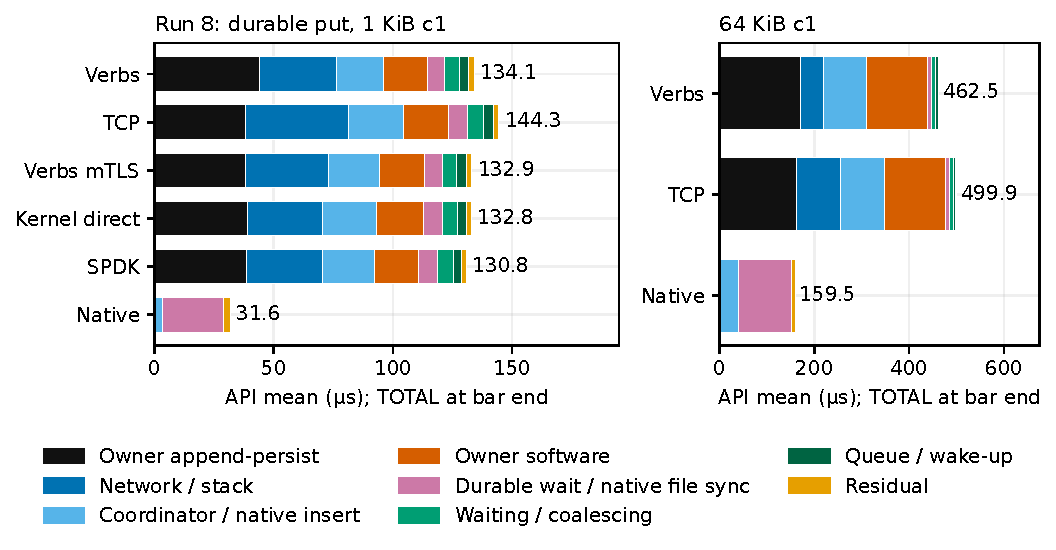
\includegraphics[width=\linewidth]{figures/durable-components.pdf}
\caption{\rEight. Mean components of durable c1 puts; one profiled repetition per route. Owner tiers are synchronous; native uses the barrier. Total at each bar end is the API mean of that same case. Each component retains the CSV label and source in \texttt{evidence.json}. The native file-sync component is in the durable-wait colour, not owner persist.}
\end{figure}
\begin{table}[H]\centering\fitinput{tab-put1.tex}
\caption{Run 8, unified fleet, 1 KiB c1 durable puts. One profiled repetition per column; means and p50 in \us. A row marked n/c has no computed component.}
\end{table}
$^{a}$ Native has no coordinator. Its insert row is WAL append plus index update. Its ``durable wait'' is the file barrier only. Directory sync is not a second additive row here; the source leaves it in the residual. The sync-step table reports file plus directory directly. Do not relabel native file sync as owner persist.

Owner persist includes software as well as fdatasync; it is not physical SSD service. Network includes both stacks and wake-up. TOTAL is the same-case API mean, not a sum of p50 values.

\clearpage
\subsection{Value size and concurrency}
\begin{table}[H]\centering\fitinput{tab-put64.tex}
\caption{Run 8, unified fleet: 64 KiB c1 durable puts, one profiled repetition. Same-case API mean is TOTAL; all times are \us. Native labels follow the note above.}
\end{table}
From 1 to 64 KiB, the verbs coordinator component rises from \N{C:p1v:coordinator} to \N{C:p64v:coordinator}~\us; owner software rises from \N{C:p1v:owner} to \N{C:p64v:owner}~\us. The corresponding network components are \N{C:p1v:network} and \N{C:p64v:network}~\us. These are distinct measured cases on one fleet, not one call's decomposition by subtraction.

\textbf{Code fact.} \path{tidehunter/src/distributed/codec.rs}, \texttt{PayloadHasher} and \texttt{record\_digest}, computes a BLAKE2b-256 digest over the full encoded payload (header prefix and encoded members). \inference\ Hashing can contribute to size-dependent software cost. These profiles do not isolate that cost. Add a stage timer or a micro-benchmark before attributing the growth to hashing. A digest change affects the wire and persisted format; ask before changing it.

\begin{table}[H]\centering\fitinput{tab-put16.tex}
\caption{Run 8, unified fleet: 1 KiB c16 durable puts. Verbs and TCP use the timeline copies, not the write-profile copies. Native uses its write profile. One repetition; \us. Shared envelopes leave owner and network unsplit. TOTAL is the API mean of the same case.}
\end{table}
At c16, waiting, queueing and durable observation dominate the timeline. The verbs exchange remains \N{C:p16v:exchange}~\us, but its three named waits are \N{C:p16v:durable}, \N{C:p16v:coalescing} and \N{C:p16v:queue}~\us. These intervals have disjoint coordinator endpoints. They are not three physical device operations. The table does not combine the separately sampled write-profile copy with the timeline copy.

\clearpage
\subsection{Owner hand-offs and nested annotations}
\begin{table}[H]\centering\fitinput{tab-owner-stages.tex}
\caption{Run 8, unified fleet: owner-clock stage mean/p50 in \us, one timeline repetition with 4,096 records per column. These are nested annotations, not an additive decomposition. No TOTAL is defined for the listed fields.}
\end{table}
The exported control queue already includes appender and flusher waits. Adding all three double counts. Handler starts after appender dequeue and includes the flusher wait. Validation and descriptor preparation are nested in append-WAL. Per record, unassigned owner time is handler minus flusher queue, append-WAL and append-persist: \N{A:v1:handler_remainder_ns:mean_us|.2f}~\us\ at 1 KiB and \N{A:v64:handler_remainder_ns:mean_us|.2f}~\us\ at 64 KiB. It covers append decode, group build and other untimed handler work. Request decode occurs before dispatch; response encoding occurs after handler completion. Neither belongs in this remainder.

\begin{table}[H]\centering\fitinput{tab-owner-profile.tex}
\caption{Separate execution: run 8, unified fleet, verbs synchronous 1 KiB c1 write-profile case \texttt{G12D-r0-0ce5f8eaa8fde37f6566}, one repetition. Totals are normalized by 4,096 sampled writes, except control queue by 4,116 samples. Connection counters can include control requests. These nested means are not additive timeline leaves.}
\end{table}
Locks and publication together cost \N{P:locks_publication_sum_ns:mean_us|.2f}~\us\ per sampled write. Connection append-persist is \N{P:connection_append_persist_ns:mean_us|.2f}~\us; storage persist is \N{P:storage_persist_total_ns:mean_us|.2f}~\us. \inference\ The approximately \N{E:profile_persist_gap|.0f}~\us\ gap is hand-off and wake-up around the flusher and durable-frontier wait, not lock time. The separate profile's append decode, group build and request/response codec sum is \N{P:codec_sum_ns:mean_us|.2f}~\us, numerically close to the timeline remainder \N{A:v1:handler_remainder_ns:mean_us|.2f}~\us. This cross-execution check has unmatched scopes: request/response codec is outside the handler. It does not explain the remainder or validate a decomposition. At 64 KiB these profile stages were not measured. Add verbs and TCP 64 KiB write-profile copies (two cases), then isolate \texttt{record\_digest} before attributing growth to BLAKE2b.

\clearpage
\subsection{Delete and batch writes}
\begin{table}[H]\centering\fitinput{tab-delete.tex}
\caption{Run 8, unified fleet: 1 KiB delete at c1, synchronous owner or native barrier. One profiled repetition. Same-case TOTAL and API p50, \us. Native ``insert'' label denotes its library operation, here delete.}
\end{table}
\begin{table}[H]\centering\fitinput{tab-batch.tex}
\caption{Run 8, unified fleet: one batch of 32 values of 8 KiB at c1, synchronous owner. One timeline repetition. Same-case TOTAL and p50, \us. The native batch has no profiler and is shown below only as a whole call.}
\end{table}
\begin{center}\small
\begin{tabular}{lrr}\toprule
Unprofiled batch, 32 values, c1 & Native barrier p50, \us & Verbs synchronous p50, \us\\\midrule
1 KiB values & \N{D:batch1n:p50_us} & \N{D:batch1v:p50_us}\\
8 KiB values & \N{D:batch8n:p50_us} & \N{D:ubatch8v:p50_us}\\\bottomrule
\end{tabular}
\end{center}
These controls each run once on the unified fleet. The appendix records the complete batch and delete populations, including page-cache acknowledgement and c16. Native batch components are not computed. TCP has a profiled 8 KiB batch, not an unprofiled batch control. Hybrid has no batch or delete case; verbs mTLS has no delete case. No batch-read result exists in these runs.

\clearpage
\section{Where the time goes: reads}\label{sec:reads}
\begin{figure}[H]\centering
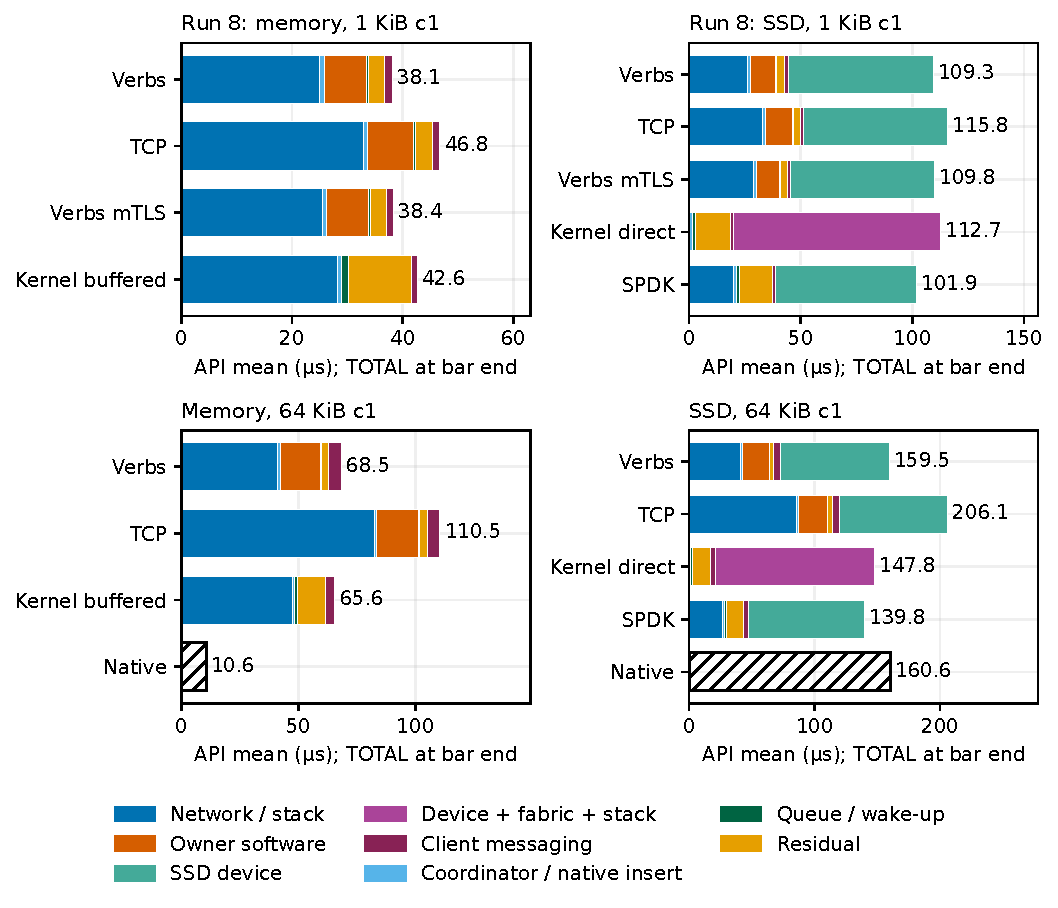
\includegraphics[width=\linewidth]{figures/read-components.pdf}
\caption{\rEight. Reads at c1, by serving-node memory or requested cold state and value size. Owner and hybrid points are one profiled repetition. Native 64 KiB bars are whole-call means (median of two per-repetition means); hatching means no decomposition. Every stacked bar prints TOTAL. Native 1 KiB memory is absent; native cold 1 KiB is unqualified.}
\end{figure}
In the WAL-read profile,
\[
T_{\mathrm{network}}=T_{\mathrm{exchange}}-T_{\mathrm{handler}}-T_{\mathrm{encode}}-T_{\mathrm{decode}}-T_{\mathrm{verify}}.
\]
All terms are mean durations in \us\ under the profile's coverage conditions. The exchange contains the subtracted stages. The separate client-messaging component counts encode, decode and verify once, not twice. Network is wire plus software in both stacks, dispatch and wake-up; no isolated wire timer exists here.

Kernel-direct device counters include non-API reads. Its device, fabric and stack interval therefore stays combined. SPDK uses its bdev latency for the device component. The residual is unattributed client time, not proof of any particular cause. The following tables retain every computed leaf and the same-case API TOTAL.

\clearpage
\subsection{Serving-node memory}
\begin{table}[H]\centering\fitinput{tab-mem1.tex}
\caption{Run 8, unified fleet: memory 1 KiB c1, one read-profile repetition, coordinator cache off. Values are mean \us, then same-case TOTAL and p50. Kernel is buffered.}
\end{table}
\begin{table}[H]\centering\fitinput{tab-mem64.tex}
\caption{Run 8, unified fleet: memory 64 KiB c1. Owner and kernel: one profiled repetition. Native: whole-call statistics, median of two repetitions, no read profiler. Its components are n/c. Values are \us.}
\end{table}
``Cache read'' here means that the serving node's memory supplies the value. It is not a coordinator RAM-cache hit. The owner verbs API mean is \N{D:mem1v:mean_us}~\us\ at 1 KiB and \N{D:mem64v:mean_us}~\us\ at 64 KiB. Native's one-process resident-oriented workload reference has 64 KiB p50 \N{D:mem64n:p50_us}~\us. Different topology and cache paths prevent a general latency lower-bound claim.

The kernel-buffered residual is \N{C:mem1k:residual}~\us\ at 1 KiB. It includes work outside the retained coordinator and reader leaves. \inference\ A client completion or dispatch change could reduce it. A call-linked stage trace must identify the work first. Do not assign it to the SSD on this memory path.

The mTLS verbs 1 KiB memory control has p50 \N{D:mem1m:p50_us}~\us, against \N{D:mem1v:p50_us}~\us\ for trusted verbs. Both are single profiled repetitions. They do not establish a statistically significant TLS penalty.

\clearpage
\subsection{SSD-served reads and native cold qualification}
\begin{table}[H]\centering\fitinput{tab-ssd1.tex}
\caption{Run 8, unified fleet: cold 1 KiB c1, one read-profile repetition. Owner reads are buffered misses; kernel direct and SPDK bypass the target page cache. TOTAL and p50 are from the same case, \us. Native is unqualified and has no computed device split.}
\end{table}
\begin{table}[H]\centering\fitinput{tab-ssd64.tex}
\caption{Run 8, unified fleet: cold 64 KiB c1, one profiled owner/hybrid repetition; native whole-call median of two repetitions. All times are \us. Native device components are n/c, not inferred from window counters.}
\end{table}
\textbf{Native correction.} Native cold 1 KiB cases are unqualified. The 8 KiB cases pass the device-count gate but have mainly memory-like latency. The 64 KiB cases meet the case-level SSD-service qualification: about \N{D:ssd64n:device_reads_per_call|.2f} device reads per API call. Native reads recent fragments through the memory map and older fragments with positional reads. \inference\ Read-ahead of mapped faults or buffered positional reads can increase device transfer sizes. Window counters do not prove that every call reached NAND; the measurement-only mapped/positional split is not measured. The owner reads the exact value range.

Native 64 KiB p50 is \N{D:ssd64n:p50_us}~\us. The direct 64 KiB SSD floor is \N{F:65536:2147483648:fresh:0:p50_us}~\us. \inference\ Native's whole call is near the floor plus about \N{E:native_read_floor_gap|.0f}~\us; this descriptive difference of separate populations is not an additive native device/software decomposition. Keep native unchanged. Any read-pattern work belongs in the distributed stack.

The owner device component is \N{C:ssd1v:device}~\us\ at 1 KiB and \N{C:ssd64v:device}~\us\ at 64 KiB, near the measured read floors. Native and owner device \emph{operations} differ in size and count; compare API calls, not device latency per operation. c16 read profiles cover only part of the reads and stay unsplit; the appendix gives their whole calls.

\clearpage
\section{Two-VM remote reads and writes (run 9)}\label{sec:rwc}
\textbf{\RWCstate} \RWCFINDING{parity}

\textbf{Topology and parity.} Selection \texttt{remote\_rw\_compact} uses one coordinator and one remote shard-WAL VM, both \texttt{z4m-highmem-16}, in \texttt{us-central1-a} with compact placement. Native runs in process on the coordinator SSD; owner TCP/verbs use the remote owner SSD. Workloads match size, caller count and repetition; read arms also match keys/order, geometry, distribution, operation/warmup counts, mix, read tier and zero coordinator-cache bytes within each temperature. Network/security, index/history, routing and host SSD remain different. Run-9 TCP used mutual TLS and verbs trusted/no TLS, so their ratios include the security difference; run 10 adds trusted TCP rather than treating run 9 as like-for-like transport evidence.

\textbf{Lanes and acknowledgement.} Native has zero remote-read lanes (in-process). Each owner uses one lane at c1/c5 and four at c16. Thus c5 owner reads are lane-limited, \emph{not a transport limit or a basis to rank transports}. Native page cache is not durable; Native per-put file/directory fsync, grouped Native barrier and owner covering file fdatasync remain distinct. Similar durable intent does not establish equal crash recovery; RF1 is not failover.

Cold eligibility requires a qualified receipt and at least 0.9 device reads per successful call, not a cache drop alone. This is a case-level proxy, not every-call NAND proof. Native 1 KiB is unqualified at all reader counts and both repetitions; Native 8/64 KiB and every owner cold cell qualify. Warm reads prewarm the serving-node page cache, not the coordinator cache. Cold/warm geometry differs; their contrast is descriptive. No calls, repetitions or fleets are pooled.
\begin{figure}[H]\centering\RWCfigure{parity}
\caption{Run-9 availability: pairs in the first two columns, distinct main-grid cases in the last three. Failed network floors are separate from KV cases. Each owner write has three Native acknowledgement controls, not three equivalent durability contracts.}
\end{figure}
\begin{table}[H]\centering\small\setlength{\tabcolsep}{3pt}
\begin{tabular}{lrrrrr}\toprule
Grid / rep. & Matched pairs & Missing pairs & Failed cases & Unqual. cases & Other cases\\\midrule
Write / r0 & \N{RWC:availability:G14O1:0:matched} & \N{RWC:availability:G14O1:0:missing partner} & \N{RWC:availability:G14O1:0:failed} & \N{RWC:availability:G14O1:0:unqualified cold} & \N{RWC:availability:G14O1:0:not available}\\
Write / r1 & \N{RWC:availability:G14O1:1:matched} & \N{RWC:availability:G14O1:1:missing partner} & \N{RWC:availability:G14O1:1:failed} & \N{RWC:availability:G14O1:1:unqualified cold} & \N{RWC:availability:G14O1:1:not available}\\
Cold read / r0 & \N{RWC:availability:G15C:0:matched} & \N{RWC:availability:G15C:0:missing partner} & \N{RWC:availability:G15C:0:failed} & \N{RWC:availability:G15C:0:unqualified cold} & \N{RWC:availability:G15C:0:not available}\\
Cold read / r1 & \N{RWC:availability:G15C:1:matched} & \N{RWC:availability:G15C:1:missing partner} & \N{RWC:availability:G15C:1:failed} & \N{RWC:availability:G15C:1:unqualified cold} & \N{RWC:availability:G15C:1:not available}\\
Warm read / r0 & \N{RWC:availability:G15M:0:matched} & \N{RWC:availability:G15M:0:missing partner} & \N{RWC:availability:G15M:0:failed} & \N{RWC:availability:G15M:0:unqualified cold} & \N{RWC:availability:G15M:0:not available}\\
Warm read / r1 & \N{RWC:availability:G15M:1:matched} & \N{RWC:availability:G15M:1:missing partner} & \N{RWC:availability:G15M:1:failed} & \N{RWC:availability:G15M:1:unqualified cold} & \N{RWC:availability:G15M:1:not available}\\
\bottomrule\end{tabular}
\caption{Separate controls: Class A Native page cache; Class B Native barriers and owner sync. No cross-class ranking. First two columns count pairs; last three distinct main-grid cases including Native. An owner write has three Native controls, an owner read one. Columns are not a partition. The three failed network-floor cases are separate, not failed KV calls. All sizes and c1/c5/c16 included; pairing does not equalize read lanes or durability. Unmatched dimensions: sync/grouping, RPC/security, index/routing, and host SSD (Native coordinator SSD versus owner SSD). Read lanes: Native 0, owner 1 at c1/c5 and 4 at c16; c5 owner reads are lane-limited, not a transport ranking. Floors are separate populations.}
\end{table}


\clearpage
\subsection{Matched writes: size and acknowledgement}
\begin{figure}[H]\centering\RWCfigure{write-latency}
\caption{Equal writers within each panel; p50 lines and p99 crosses, repetitions separate. Native page cache is non-durable context; other arms wait for per-put, grouped or covering sync. One data SSD per arm, on different hosts.}
\end{figure}
\begin{table}[H]\centering\small\setlength{\tabcolsep}{3pt}
\begin{tabular}{lrrrrr}\toprule
Size & Arm & Rep. & c1 & c5 & c16\\\midrule
1 KiB & Native page cache & r0 & \N{RWC:latency_vs_size:17:p50_us:1|.2f}/\N{RWC:latency_vs_size:17:p99_us:1|.2f} & \N{RWC:latency_vs_size:27:p50_us:1|.2f}/\N{RWC:latency_vs_size:27:p99_us:1|.2f} & \N{RWC:latency_vs_size:37:p50_us:1|.2f}/\N{RWC:latency_vs_size:37:p99_us:1|.2f}\\
1 KiB & Native page cache & r1 & \N{RWC:latency_vs_size:26:p50_us:1|.2f}/\N{RWC:latency_vs_size:26:p99_us:1|.2f} & \N{RWC:latency_vs_size:36:p50_us:1|.2f}/\N{RWC:latency_vs_size:36:p99_us:1|.2f} & \N{RWC:latency_vs_size:46:p50_us:1|.2f}/\N{RWC:latency_vs_size:46:p99_us:1|.2f}\\
1 KiB & Native per-put barrier & r0 & \N{RWC:latency_vs_size:18:p50_us:1|.1f}/\N{RWC:latency_vs_size:18:p99_us:1|.1f} & \N{RWC:latency_vs_size:28:p50_us:1|.1f}/\N{RWC:latency_vs_size:28:p99_us:1|.0f} & \N{RWC:latency_vs_size:38:p50_us:1|.1f}/\N{RWC:latency_vs_size:38:p99_us:1|.0f}\\
1 KiB & Native per-put barrier & r1 & \N{RWC:latency_vs_size:25:p50_us:1|.1f}/\N{RWC:latency_vs_size:25:p99_us:1|.1f} & \N{RWC:latency_vs_size:35:p50_us:1|.1f}/\N{RWC:latency_vs_size:35:p99_us:1|.0f} & \N{RWC:latency_vs_size:45:p50_us:1|.1f}/\N{RWC:latency_vs_size:45:p99_us:1|.0f}\\
1 KiB & Native grouped barrier & r0 & \N{RWC:latency_vs_size:19:p50_us:1|.1f}/\N{RWC:latency_vs_size:19:p99_us:1|.1f} & \N{RWC:latency_vs_size:29:p50_us:1|.1f}/\N{RWC:latency_vs_size:29:p99_us:1|.0f} & \N{RWC:latency_vs_size:39:p50_us:1|.1f}/\N{RWC:latency_vs_size:39:p99_us:1|.0f}\\
1 KiB & Native grouped barrier & r1 & \N{RWC:latency_vs_size:24:p50_us:1|.1f}/\N{RWC:latency_vs_size:24:p99_us:1|.1f} & \N{RWC:latency_vs_size:34:p50_us:1|.1f}/\N{RWC:latency_vs_size:34:p99_us:1|.0f} & \N{RWC:latency_vs_size:44:p50_us:1|.1f}/\N{RWC:latency_vs_size:44:p99_us:1|.0f}\\
1 KiB & Owner TCP & r0 & \N{RWC:latency_vs_size:20:p50_us:1|.0f}/\N{RWC:latency_vs_size:20:p99_us:1|.0f} & \N{RWC:latency_vs_size:30:p50_us:1|.0f}/\N{RWC:latency_vs_size:30:p99_us:1|.0f} & \N{RWC:latency_vs_size:40:p50_us:1|.0f}/\N{RWC:latency_vs_size:40:p99_us:1|.0f}\\
1 KiB & Owner TCP & r1 & \N{RWC:latency_vs_size:23:p50_us:1|.0f}/\N{RWC:latency_vs_size:23:p99_us:1|.0f} & \N{RWC:latency_vs_size:33:p50_us:1|.0f}/\N{RWC:latency_vs_size:33:p99_us:1|.0f} & \N{RWC:latency_vs_size:43:p50_us:1|.0f}/\N{RWC:latency_vs_size:43:p99_us:1|.0f}\\
1 KiB & Owner verbs & r0 & \N{RWC:latency_vs_size:21:p50_us:1|.0f}/\N{RWC:latency_vs_size:21:p99_us:1|.0f} & \N{RWC:latency_vs_size:31:p50_us:1|.0f}/\N{RWC:latency_vs_size:31:p99_us:1|.0f} & \N{RWC:latency_vs_size:41:p50_us:1|.0f}/\N{RWC:latency_vs_size:41:p99_us:1|.0f}\\
1 KiB & Owner verbs & r1 & \N{RWC:latency_vs_size:22:p50_us:1|.0f}/\N{RWC:latency_vs_size:22:p99_us:1|.0f} & \N{RWC:latency_vs_size:32:p50_us:1|.0f}/\N{RWC:latency_vs_size:32:p99_us:1|.0f} & \N{RWC:latency_vs_size:42:p50_us:1|.0f}/\N{RWC:latency_vs_size:42:p99_us:1|.0f}\\
8 KiB & Native page cache & r0 & \N{RWC:latency_vs_size:47:p50_us:1|.2f}/\N{RWC:latency_vs_size:47:p99_us:1|.2f} & \N{RWC:latency_vs_size:57:p50_us:1|.2f}/\N{RWC:latency_vs_size:57:p99_us:1|.2f} & \N{RWC:latency_vs_size:67:p50_us:1|.2f}/\N{RWC:latency_vs_size:67:p99_us:1|.2f}\\
8 KiB & Native page cache & r1 & \N{RWC:latency_vs_size:56:p50_us:1|.2f}/\N{RWC:latency_vs_size:56:p99_us:1|.2f} & \N{RWC:latency_vs_size:66:p50_us:1|.2f}/\N{RWC:latency_vs_size:66:p99_us:1|.2f} & \N{RWC:latency_vs_size:76:p50_us:1|.2f}/\N{RWC:latency_vs_size:76:p99_us:1|.2f}\\
8 KiB & Native per-put barrier & r0 & \N{RWC:latency_vs_size:48:p50_us:1|.1f}/\N{RWC:latency_vs_size:48:p99_us:1|.1f} & \N{RWC:latency_vs_size:58:p50_us:1|.1f}/\N{RWC:latency_vs_size:58:p99_us:1|.0f} & \N{RWC:latency_vs_size:68:p50_us:1|.0f}/\N{RWC:latency_vs_size:68:p99_us:1|.0f}\\
8 KiB & Native per-put barrier & r1 & \N{RWC:latency_vs_size:55:p50_us:1|.1f}/\N{RWC:latency_vs_size:55:p99_us:1|.1f} & \N{RWC:latency_vs_size:65:p50_us:1|.1f}/\N{RWC:latency_vs_size:65:p99_us:1|.0f} & \N{RWC:latency_vs_size:75:p50_us:1|.0f}/\N{RWC:latency_vs_size:75:p99_us:1|.0f}\\
8 KiB & Native grouped barrier & r0 & \N{RWC:latency_vs_size:49:p50_us:1|.1f}/\N{RWC:latency_vs_size:49:p99_us:1|.1f} & \N{RWC:latency_vs_size:59:p50_us:1|.1f}/\N{RWC:latency_vs_size:59:p99_us:1|.0f} & \N{RWC:latency_vs_size:69:p50_us:1|.0f}/\N{RWC:latency_vs_size:69:p99_us:1|.0f}\\
8 KiB & Native grouped barrier & r1 & \N{RWC:latency_vs_size:54:p50_us:1|.1f}/\N{RWC:latency_vs_size:54:p99_us:1|.1f} & \N{RWC:latency_vs_size:64:p50_us:1|.1f}/\N{RWC:latency_vs_size:64:p99_us:1|.0f} & \N{RWC:latency_vs_size:74:p50_us:1|.0f}/\N{RWC:latency_vs_size:74:p99_us:1|.0f}\\
8 KiB & Owner TCP & r0 & \N{RWC:latency_vs_size:50:p50_us:1|.0f}/\N{RWC:latency_vs_size:50:p99_us:1|.0f} & \N{RWC:latency_vs_size:60:p50_us:1|.0f}/\N{RWC:latency_vs_size:60:p99_us:1|.0f} & \N{RWC:latency_vs_size:70:p50_us:1|.0f}/\N{RWC:latency_vs_size:70:p99_us:1|.0f}\\
8 KiB & Owner TCP & r1 & \N{RWC:latency_vs_size:53:p50_us:1|.0f}/\N{RWC:latency_vs_size:53:p99_us:1|.0f} & \N{RWC:latency_vs_size:63:p50_us:1|.0f}/\N{RWC:latency_vs_size:63:p99_us:1|.0f} & \N{RWC:latency_vs_size:73:p50_us:1|.0f}/\N{RWC:latency_vs_size:73:p99_us:1|.0f}\\
8 KiB & Owner verbs & r0 & \N{RWC:latency_vs_size:51:p50_us:1|.0f}/\N{RWC:latency_vs_size:51:p99_us:1|.0f} & \N{RWC:latency_vs_size:61:p50_us:1|.0f}/\N{RWC:latency_vs_size:61:p99_us:1|.0f} & \N{RWC:latency_vs_size:71:p50_us:1|.0f}/\N{RWC:latency_vs_size:71:p99_us:1|.0f}\\
8 KiB & Owner verbs & r1 & \N{RWC:latency_vs_size:52:p50_us:1|.0f}/\N{RWC:latency_vs_size:52:p99_us:1|.0f} & \N{RWC:latency_vs_size:62:p50_us:1|.0f}/\N{RWC:latency_vs_size:62:p99_us:1|.0f} & \N{RWC:latency_vs_size:72:p50_us:1|.0f}/\N{RWC:latency_vs_size:72:p99_us:1|.0f}\\
64 KiB & Native page cache & r0 & \N{RWC:latency_vs_size:77:p50_us:1|.1f}/\N{RWC:latency_vs_size:77:p99_us:1|.1f} & \N{RWC:latency_vs_size:87:p50_us:1|.1f}/\N{RWC:latency_vs_size:87:p99_us:1|.0f} & \N{RWC:latency_vs_size:12:p50_us:1|.0f}/\N{RWC:latency_vs_size:12:p99_us:1|.0f}\\
64 KiB & Native page cache & r1 & \N{RWC:latency_vs_size:86:p50_us:1|.1f}/\N{RWC:latency_vs_size:86:p99_us:1|.0f} & \N{RWC:latency_vs_size:96:p50_us:1|.1f}/\N{RWC:latency_vs_size:96:p99_us:1|.0f} & \N{RWC:latency_vs_size:101:p50_us:1|.0f}/\N{RWC:latency_vs_size:101:p99_us:1|.0f}\\
64 KiB & Native per-put barrier & r0 & \N{RWC:latency_vs_size:78:p50_us:1|.0f}/\N{RWC:latency_vs_size:78:p99_us:1|.0f} & \N{RWC:latency_vs_size:88:p50_us:1|.0f}/\N{RWC:latency_vs_size:88:p99_us:1|.0f} & \N{RWC:latency_vs_size:13:p50_us:1|.0f}/\N{RWC:latency_vs_size:13:p99_us:1|.0f}\\
64 KiB & Native per-put barrier & r1 & \N{RWC:latency_vs_size:85:p50_us:1|.0f}/\N{RWC:latency_vs_size:85:p99_us:1|.0f} & \N{RWC:latency_vs_size:95:p50_us:1|.0f}/\N{RWC:latency_vs_size:95:p99_us:1|.0f} & \N{RWC:latency_vs_size:100:p50_us:1|.0f}/\N{RWC:latency_vs_size:100:p99_us:1|.0f}\\
64 KiB & Native grouped barrier & r0 & \N{RWC:latency_vs_size:79:p50_us:1|.0f}/\N{RWC:latency_vs_size:79:p99_us:1|.0f} & \N{RWC:latency_vs_size:89:p50_us:1|.0f}/\N{RWC:latency_vs_size:89:p99_us:1|.0f} & \N{RWC:latency_vs_size:14:p50_us:1|.0f}/\N{RWC:latency_vs_size:14:p99_us:1|.0f}\\
64 KiB & Native grouped barrier & r1 & \N{RWC:latency_vs_size:84:p50_us:1|.0f}/\N{RWC:latency_vs_size:84:p99_us:1|.0f} & \N{RWC:latency_vs_size:94:p50_us:1|.0f}/\N{RWC:latency_vs_size:94:p99_us:1|.0f} & \N{RWC:latency_vs_size:99:p50_us:1|.0f}/\N{RWC:latency_vs_size:99:p99_us:1|.0f}\\
64 KiB & Owner TCP & r0 & \N{RWC:latency_vs_size:80:p50_us:1|.0f}/\N{RWC:latency_vs_size:80:p99_us:1|.0f} & \N{RWC:latency_vs_size:90:p50_us:1|.0f}/\N{RWC:latency_vs_size:90:p99_us:1|.0f} & \N{RWC:latency_vs_size:15:p50_us:1|.0f}/\N{RWC:latency_vs_size:15:p99_us:1|.0f}\\
64 KiB & Owner TCP & r1 & \N{RWC:latency_vs_size:83:p50_us:1|.0f}/\N{RWC:latency_vs_size:83:p99_us:1|.0f} & \N{RWC:latency_vs_size:93:p50_us:1|.0f}/\N{RWC:latency_vs_size:93:p99_us:1|.0f} & \N{RWC:latency_vs_size:98:p50_us:1|.0f}/\N{RWC:latency_vs_size:98:p99_us:1|.0f}\\
64 KiB & Owner verbs & r0 & \N{RWC:latency_vs_size:81:p50_us:1|.0f}/\N{RWC:latency_vs_size:81:p99_us:1|.0f} & \N{RWC:latency_vs_size:91:p50_us:1|.0f}/\N{RWC:latency_vs_size:91:p99_us:1|.0f} & \N{RWC:latency_vs_size:16:p50_us:1|.0f}/\N{RWC:latency_vs_size:16:p99_us:1|.0f}\\
64 KiB & Owner verbs & r1 & \N{RWC:latency_vs_size:82:p50_us:1|.0f}/\N{RWC:latency_vs_size:82:p99_us:1|.0f} & \N{RWC:latency_vs_size:92:p50_us:1|.0f}/\N{RWC:latency_vs_size:92:p99_us:1|.0f} & \N{RWC:latency_vs_size:97:p50_us:1|.0f}/\N{RWC:latency_vs_size:97:p99_us:1|.0f}\\
\bottomrule\end{tabular}
\caption{Writes; successful API p50/p99 (\us{}), one row per repetition, never pooled. All three caller counts are shown. Values below 10 use two decimals, below 100 one, otherwise whole microseconds. Native page-cache writes are not durable; barrier/grouped/covering sync remain distinct. Unmatched dimensions: sync/grouping, RPC/security, index/routing, and host SSD (Native coordinator SSD versus owner SSD). Read lanes: Native 0, owner 1 at c1/c5 and 4 at c16; c5 owner reads are lane-limited, not a transport ranking. Floors are separate populations.}
\end{table}

\RWCFINDING{writes}

\clearpage
\subsection{Matched reads: device-qualified and prewarmed}
\begin{figure}[H]\centering\RWCfigure{read-latency}
\caption{Matched readers, sizes and repetitions; coordinator cache off. Unqualified Native cold 1 KiB has no latency marker. Native is in process; owners use one lane at c1, four at c16. Appendix~\ref{app:rwc-qualification} retains every verdict and device ratio, including c5.}
\end{figure}
\begin{table}[H]\centering\small\setlength{\tabcolsep}{3pt}
\begin{tabular}{lrrrrr}\toprule
Size & Arm & Rep. & c1 & c5* & c16\\\midrule
1 KiB & Native & r0 & unqualified & unqualified & unqualified\\
1 KiB & Native & r1 & unqualified & unqualified & unqualified\\
1 KiB & Owner TCP & r0 & \N{RWC:latency_vs_size:1:p50_us:1|.0f}/\N{RWC:latency_vs_size:1:p99_us:1|.0f} & \N{RWC:latency_vs_size:106:p50_us:1|.0f}/\N{RWC:latency_vs_size:106:p99_us:1|.0f} & \N{RWC:latency_vs_size:112:p50_us:1|.0f}/\N{RWC:latency_vs_size:112:p99_us:1|.0f}\\
1 KiB & Owner TCP & r1 & \N{RWC:latency_vs_size:103:p50_us:1|.0f}/\N{RWC:latency_vs_size:103:p99_us:1|.0f} & \N{RWC:latency_vs_size:109:p50_us:1|.0f}/\N{RWC:latency_vs_size:109:p99_us:1|.0f} & \N{RWC:latency_vs_size:115:p50_us:1|.0f}/\N{RWC:latency_vs_size:115:p99_us:1|.0f}\\
1 KiB & Owner verbs & r0 & \N{RWC:latency_vs_size:2:p50_us:1|.0f}/\N{RWC:latency_vs_size:2:p99_us:1|.0f} & \N{RWC:latency_vs_size:107:p50_us:1|.0f}/\N{RWC:latency_vs_size:107:p99_us:1|.0f} & \N{RWC:latency_vs_size:113:p50_us:1|.0f}/\N{RWC:latency_vs_size:113:p99_us:1|.0f}\\
1 KiB & Owner verbs & r1 & \N{RWC:latency_vs_size:102:p50_us:1|.0f}/\N{RWC:latency_vs_size:102:p99_us:1|.0f} & \N{RWC:latency_vs_size:108:p50_us:1|.0f}/\N{RWC:latency_vs_size:108:p99_us:1|.0f} & \N{RWC:latency_vs_size:114:p50_us:1|.0f}/\N{RWC:latency_vs_size:114:p99_us:1|.0f}\\
8 KiB & Native & r0 & \N{RWC:latency_vs_size:117:p50_us:1|.2f}/\N{RWC:latency_vs_size:117:p99_us:1|.0f} & \N{RWC:latency_vs_size:123:p50_us:1|.2f}/\N{RWC:latency_vs_size:123:p99_us:1|.0f} & \N{RWC:latency_vs_size:129:p50_us:1|.2f}/\N{RWC:latency_vs_size:129:p99_us:1|.0f}\\
8 KiB & Native & r1 & \N{RWC:latency_vs_size:122:p50_us:1|.2f}/\N{RWC:latency_vs_size:122:p99_us:1|.0f} & \N{RWC:latency_vs_size:128:p50_us:1|.2f}/\N{RWC:latency_vs_size:128:p99_us:1|.0f} & \N{RWC:latency_vs_size:134:p50_us:1|.2f}/\N{RWC:latency_vs_size:134:p99_us:1|.0f}\\
8 KiB & Owner TCP & r0 & \N{RWC:latency_vs_size:118:p50_us:1|.0f}/\N{RWC:latency_vs_size:118:p99_us:1|.0f} & \N{RWC:latency_vs_size:124:p50_us:1|.0f}/\N{RWC:latency_vs_size:124:p99_us:1|.0f} & \N{RWC:latency_vs_size:130:p50_us:1|.0f}/\N{RWC:latency_vs_size:130:p99_us:1|.0f}\\
8 KiB & Owner TCP & r1 & \N{RWC:latency_vs_size:121:p50_us:1|.0f}/\N{RWC:latency_vs_size:121:p99_us:1|.0f} & \N{RWC:latency_vs_size:127:p50_us:1|.0f}/\N{RWC:latency_vs_size:127:p99_us:1|.0f} & \N{RWC:latency_vs_size:133:p50_us:1|.0f}/\N{RWC:latency_vs_size:133:p99_us:1|.0f}\\
8 KiB & Owner verbs & r0 & \N{RWC:latency_vs_size:119:p50_us:1|.0f}/\N{RWC:latency_vs_size:119:p99_us:1|.0f} & \N{RWC:latency_vs_size:125:p50_us:1|.0f}/\N{RWC:latency_vs_size:125:p99_us:1|.0f} & \N{RWC:latency_vs_size:131:p50_us:1|.0f}/\N{RWC:latency_vs_size:131:p99_us:1|.0f}\\
8 KiB & Owner verbs & r1 & \N{RWC:latency_vs_size:120:p50_us:1|.0f}/\N{RWC:latency_vs_size:120:p99_us:1|.0f} & \N{RWC:latency_vs_size:126:p50_us:1|.0f}/\N{RWC:latency_vs_size:126:p99_us:1|.0f} & \N{RWC:latency_vs_size:132:p50_us:1|.0f}/\N{RWC:latency_vs_size:132:p99_us:1|.0f}\\
64 KiB & Native & r0 & \N{RWC:latency_vs_size:135:p50_us:1|.0f}/\N{RWC:latency_vs_size:135:p99_us:1|.0f} & \N{RWC:latency_vs_size:141:p50_us:1|.0f}/\N{RWC:latency_vs_size:141:p99_us:1|.0f} & \N{RWC:latency_vs_size:6:p50_us:1|.0f}/\N{RWC:latency_vs_size:6:p99_us:1|.0f}\\
64 KiB & Native & r1 & \N{RWC:latency_vs_size:140:p50_us:1|.1f}/\N{RWC:latency_vs_size:140:p99_us:1|.0f} & \N{RWC:latency_vs_size:146:p50_us:1|.0f}/\N{RWC:latency_vs_size:146:p99_us:1|.0f} & \N{RWC:latency_vs_size:149:p50_us:1|.0f}/\N{RWC:latency_vs_size:149:p99_us:1|.0f}\\
64 KiB & Owner TCP & r0 & \N{RWC:latency_vs_size:136:p50_us:1|.0f}/\N{RWC:latency_vs_size:136:p99_us:1|.0f} & \N{RWC:latency_vs_size:142:p50_us:1|.0f}/\N{RWC:latency_vs_size:142:p99_us:1|.0f} & \N{RWC:latency_vs_size:7:p50_us:1|.0f}/\N{RWC:latency_vs_size:7:p99_us:1|.0f}\\
64 KiB & Owner TCP & r1 & \N{RWC:latency_vs_size:139:p50_us:1|.0f}/\N{RWC:latency_vs_size:139:p99_us:1|.0f} & \N{RWC:latency_vs_size:145:p50_us:1|.0f}/\N{RWC:latency_vs_size:145:p99_us:1|.0f} & \N{RWC:latency_vs_size:148:p50_us:1|.0f}/\N{RWC:latency_vs_size:148:p99_us:1|.0f}\\
64 KiB & Owner verbs & r0 & \N{RWC:latency_vs_size:137:p50_us:1|.0f}/\N{RWC:latency_vs_size:137:p99_us:1|.0f} & \N{RWC:latency_vs_size:143:p50_us:1|.0f}/\N{RWC:latency_vs_size:143:p99_us:1|.0f} & \N{RWC:latency_vs_size:8:p50_us:1|.0f}/\N{RWC:latency_vs_size:8:p99_us:1|.0f}\\
64 KiB & Owner verbs & r1 & \N{RWC:latency_vs_size:138:p50_us:1|.0f}/\N{RWC:latency_vs_size:138:p99_us:1|.0f} & \N{RWC:latency_vs_size:144:p50_us:1|.0f}/\N{RWC:latency_vs_size:144:p99_us:1|.0f} & \N{RWC:latency_vs_size:147:p50_us:1|.0f}/\N{RWC:latency_vs_size:147:p99_us:1|.0f}\\
\bottomrule\end{tabular}
\caption{Cold reads; successful API p50/p99 (\us{}), one row per repetition, never pooled. All three caller counts are shown. Values below 10 use two decimals, below 100 one, otherwise whole microseconds. Coordinator cache off. Unqualified cold cells have no latency. Unmatched dimensions: sync/grouping, RPC/security, index/routing, and host SSD (Native coordinator SSD versus owner SSD). Read lanes: Native 0, owner 1 at c1/c5 and 4 at c16; c5 owner reads are lane-limited, not a transport ranking. Floors are separate populations.}
\end{table}

\RWCFINDING{cold-populations}

\clearpage
\subsection{Warm reads and the cache contrast}
\begin{table}[H]\centering\small\setlength{\tabcolsep}{3pt}
\begin{tabular}{lrrrrr}\toprule
Size & Arm & Rep. & c1 & c5* & c16\\\midrule
1 KiB & Native & r0 & \N{RWC:latency_vs_size:3:p50_us:1|.2f}/\N{RWC:latency_vs_size:3:p99_us:1|.2f} & \N{RWC:latency_vs_size:153:p50_us:1|.2f}/\N{RWC:latency_vs_size:153:p99_us:1|.2f} & \N{RWC:latency_vs_size:159:p50_us:1|.2f}/\N{RWC:latency_vs_size:159:p99_us:1|.2f}\\
1 KiB & Native & r1 & \N{RWC:latency_vs_size:152:p50_us:1|.2f}/\N{RWC:latency_vs_size:152:p99_us:1|.2f} & \N{RWC:latency_vs_size:158:p50_us:1|.2f}/\N{RWC:latency_vs_size:158:p99_us:1|.2f} & \N{RWC:latency_vs_size:164:p50_us:1|.2f}/\N{RWC:latency_vs_size:164:p99_us:1|.2f}\\
1 KiB & Owner TCP & r0 & \N{RWC:latency_vs_size:5:p50_us:1|.1f}/\N{RWC:latency_vs_size:5:p99_us:1|.1f} & \N{RWC:latency_vs_size:155:p50_us:1|.0f}/\N{RWC:latency_vs_size:155:p99_us:1|.0f} & \N{RWC:latency_vs_size:161:p50_us:1|.1f}/\N{RWC:latency_vs_size:161:p99_us:1|.0f}\\
1 KiB & Owner TCP & r1 & \N{RWC:latency_vs_size:150:p50_us:1|.1f}/\N{RWC:latency_vs_size:150:p99_us:1|.1f} & \N{RWC:latency_vs_size:156:p50_us:1|.0f}/\N{RWC:latency_vs_size:156:p99_us:1|.0f} & \N{RWC:latency_vs_size:162:p50_us:1|.1f}/\N{RWC:latency_vs_size:162:p99_us:1|.0f}\\
1 KiB & Owner verbs & r0 & \N{RWC:latency_vs_size:4:p50_us:1|.1f}/\N{RWC:latency_vs_size:4:p99_us:1|.1f} & \N{RWC:latency_vs_size:154:p50_us:1|.0f}/\N{RWC:latency_vs_size:154:p99_us:1|.0f} & \N{RWC:latency_vs_size:160:p50_us:1|.1f}/\N{RWC:latency_vs_size:160:p99_us:1|.0f}\\
1 KiB & Owner verbs & r1 & \N{RWC:latency_vs_size:151:p50_us:1|.1f}/\N{RWC:latency_vs_size:151:p99_us:1|.1f} & \N{RWC:latency_vs_size:157:p50_us:1|.0f}/\N{RWC:latency_vs_size:157:p99_us:1|.0f} & \N{RWC:latency_vs_size:163:p50_us:1|.1f}/\N{RWC:latency_vs_size:163:p99_us:1|.0f}\\
8 KiB & Native & r0 & \N{RWC:latency_vs_size:165:p50_us:1|.2f}/\N{RWC:latency_vs_size:165:p99_us:1|.2f} & \N{RWC:latency_vs_size:171:p50_us:1|.2f}/\N{RWC:latency_vs_size:171:p99_us:1|.2f} & \N{RWC:latency_vs_size:177:p50_us:1|.2f}/\N{RWC:latency_vs_size:177:p99_us:1|.2f}\\
8 KiB & Native & r1 & \N{RWC:latency_vs_size:170:p50_us:1|.2f}/\N{RWC:latency_vs_size:170:p99_us:1|.2f} & \N{RWC:latency_vs_size:176:p50_us:1|.2f}/\N{RWC:latency_vs_size:176:p99_us:1|.2f} & \N{RWC:latency_vs_size:182:p50_us:1|.2f}/\N{RWC:latency_vs_size:182:p99_us:1|.2f}\\
8 KiB & Owner TCP & r0 & \N{RWC:latency_vs_size:167:p50_us:1|.1f}/\N{RWC:latency_vs_size:167:p99_us:1|.1f} & \N{RWC:latency_vs_size:173:p50_us:1|.0f}/\N{RWC:latency_vs_size:173:p99_us:1|.0f} & \N{RWC:latency_vs_size:179:p50_us:1|.0f}/\N{RWC:latency_vs_size:179:p99_us:1|.0f}\\
8 KiB & Owner TCP & r1 & \N{RWC:latency_vs_size:168:p50_us:1|.1f}/\N{RWC:latency_vs_size:168:p99_us:1|.1f} & \N{RWC:latency_vs_size:174:p50_us:1|.0f}/\N{RWC:latency_vs_size:174:p99_us:1|.0f} & \N{RWC:latency_vs_size:180:p50_us:1|.0f}/\N{RWC:latency_vs_size:180:p99_us:1|.0f}\\
8 KiB & Owner verbs & r0 & \N{RWC:latency_vs_size:166:p50_us:1|.1f}/\N{RWC:latency_vs_size:166:p99_us:1|.1f} & \N{RWC:latency_vs_size:172:p50_us:1|.0f}/\N{RWC:latency_vs_size:172:p99_us:1|.0f} & \N{RWC:latency_vs_size:178:p50_us:1|.1f}/\N{RWC:latency_vs_size:178:p99_us:1|.0f}\\
8 KiB & Owner verbs & r1 & \N{RWC:latency_vs_size:169:p50_us:1|.1f}/\N{RWC:latency_vs_size:169:p99_us:1|.1f} & \N{RWC:latency_vs_size:175:p50_us:1|.0f}/\N{RWC:latency_vs_size:175:p99_us:1|.0f} & \N{RWC:latency_vs_size:181:p50_us:1|.1f}/\N{RWC:latency_vs_size:181:p99_us:1|.0f}\\
64 KiB & Native & r0 & \N{RWC:latency_vs_size:183:p50_us:1|.1f}/\N{RWC:latency_vs_size:183:p99_us:1|.1f} & \N{RWC:latency_vs_size:189:p50_us:1|.1f}/\N{RWC:latency_vs_size:189:p99_us:1|.1f} & \N{RWC:latency_vs_size:9:p50_us:1|.1f}/\N{RWC:latency_vs_size:9:p99_us:1|.1f}\\
64 KiB & Native & r1 & \N{RWC:latency_vs_size:188:p50_us:1|.1f}/\N{RWC:latency_vs_size:188:p99_us:1|.1f} & \N{RWC:latency_vs_size:194:p50_us:1|.1f}/\N{RWC:latency_vs_size:194:p99_us:1|.1f} & \N{RWC:latency_vs_size:197:p50_us:1|.1f}/\N{RWC:latency_vs_size:197:p99_us:1|.1f}\\
64 KiB & Owner TCP & r0 & \N{RWC:latency_vs_size:185:p50_us:1|.1f}/\N{RWC:latency_vs_size:185:p99_us:1|.0f} & \N{RWC:latency_vs_size:191:p50_us:1|.0f}/\N{RWC:latency_vs_size:191:p99_us:1|.0f} & \N{RWC:latency_vs_size:11:p50_us:1|.0f}/\N{RWC:latency_vs_size:11:p99_us:1|.0f}\\
64 KiB & Owner TCP & r1 & \N{RWC:latency_vs_size:186:p50_us:1|.1f}/\N{RWC:latency_vs_size:186:p99_us:1|.0f} & \N{RWC:latency_vs_size:192:p50_us:1|.0f}/\N{RWC:latency_vs_size:192:p99_us:1|.0f} & \N{RWC:latency_vs_size:195:p50_us:1|.0f}/\N{RWC:latency_vs_size:195:p99_us:1|.0f}\\
64 KiB & Owner verbs & r0 & \N{RWC:latency_vs_size:184:p50_us:1|.1f}/\N{RWC:latency_vs_size:184:p99_us:1|.1f} & \N{RWC:latency_vs_size:190:p50_us:1|.0f}/\N{RWC:latency_vs_size:190:p99_us:1|.0f} & \N{RWC:latency_vs_size:10:p50_us:1|.0f}/\N{RWC:latency_vs_size:10:p99_us:1|.0f}\\
64 KiB & Owner verbs & r1 & \N{RWC:latency_vs_size:187:p50_us:1|.1f}/\N{RWC:latency_vs_size:187:p99_us:1|.1f} & \N{RWC:latency_vs_size:193:p50_us:1|.0f}/\N{RWC:latency_vs_size:193:p99_us:1|.0f} & \N{RWC:latency_vs_size:196:p50_us:1|.0f}/\N{RWC:latency_vs_size:196:p99_us:1|.0f}\\
\bottomrule\end{tabular}
\caption{Read preparation: Class B write settings, not a read durability guarantee. Warm reads; successful API p50/p99 (\us{}), repetitions separate; c1/c5/c16. Coordinator cache off. Unqualified cold cells have no latency. Unmatched dimensions: sync/grouping, RPC/security, index/routing, and host SSD (Native coordinator SSD versus owner SSD). Read lanes: Native 0, owner 1 at c1/c5 and 4 at c16; c5 owner reads are lane-limited, not a transport ranking. Floors are separate populations.}
\end{table}

\begin{figure}[H]\centering\RWCfigure{cold-warm}
\caption{Cold versus prewarmed whole-call means at one reader. Each point joins arm, size and repetition, but dataset geometry and operation counts differ. Shape identifies size; filled/open means r0/r1. No subtraction identifies SSD service.}
\end{figure}
\RWCFINDING{warm}

\clearpage
\subsection{Finite-case rates and the read-lane limit}
\begin{figure}[H]\centering\RWCfigure{throughput}
\caption{Successful API calls/s, not production capacity. c5 owner read points are shaded and lane-limited: one owner lane at c1/c5, four at c16; Native is in process. Do not rank transports on c5 cells. Write acknowledgement and cold/warm read contracts remain separate. Per-case in-flight, offered and unsuccessful counts remain in the CSV and figure evidence; missing occupancy is not zero.}
\end{figure}
\RWCFINDING{lanes}

\clearpage
\subsection{Floors, not an additive decomposition}
\begin{figure}[H]\centering\RWCfigure{floors}
\caption{Client/owner SSD and network floor means beside owner whole-call means, not a latency stack. Half RTT is doubled only where the receipt specifies it. Failed \texttt{ib\_write\_lat} event controls are unavailable, not zero; see Appendix~\ref{app:rwc-floors}.}
\end{figure}
\textbf{[INFERENCE]} Floors motivate hardware/software hypotheses but do not identify additive overhead. An exact partition needs disjoint, call-linked intervals from the same population; these independent controls do not supply them. No software remainder is computed.

Compare the \emph{same kind of call}: Native all-file fsync plus directory differs from owner one-file fdatasync. Append controls include fresh allocation; overwrite-fdatasync does not. Direct QD1 random reads differ from Native mapped/positional reads and owner exact-range buffered reads. Network tools do not include full RPC/security processing. Both host floors matter; equal VM class is not identical hardware.

\textbf{Limits.} One fleet and r0/r1 do not establish fleet spread or significance. Read/network floors have r0--r2; append controls r0/r1; three diagnostic profiles run once and remain separate. This run does not test five owners, NVMe-oF reads, Spot/other machine types, Sui replay, production capacity or failover. Three event-write floor failures are tool/mode failures, not system failures. The terminal report marks the campaign incomplete because of those failures; all planned cases have terminal receipts. No first-attempt result is used.

\clearpage
\section{Run 10: fabric, security and polling}\label{sec:rwc10}
\textbf{Topology and scope.} The reviewed \texttt{fabric\_ab\_compact} selection uses one coordinator VM and one remote shard-WAL VM, both \texttt{z4m-highmem-16} in \texttt{us-central1-a} with compact placement, not five owners. There are two value sizes (1 and 64 KiB), one or sixteen readers and separate r0/r1 cases. The coordinator cache is off. Ordinary owner reads traverse RPC; warm cases prewarm the serving-node page cache. Lanes are one at c1 and four at c16. Matching caller counts does not establish saturation, fleet spread or physical-device service.

\textbf{Run-9 security correction.} Run 9's TCP owner arm used mutual TLS, while its verbs arm was trusted without TLS: those TCP/verbs ratios include the security difference and are not like-for-like transport comparisons. Run 10 adds trusted TCP and keeps it distinct from mTLS. Trusted modes do not supply cryptographic peer authentication; no downgrade is proposed for an untrusted network.

\RWCtenTable{arms}
\textbf{Polling contract.} A means Adaptive; B means the Busy policy. Busy is \emph{owner spins in user space}; the coordinator read driver adopts that policy and also spins. It is not an owner-only intervention, not a guarantee that all threads never block, and not kernel socket busy polling. \texttt{SO\_BUSY\_POLL} is not wired in the engine. The raw run-9 socket floor that uses it remains a different experiment.

\textbf{Measurements and absent evidence.} API latency covers successful calls; the CSVs retain successful counts, offered/unsuccessful calls, finite-case rates, observed in-flight calls, process CPU, CQ waits, statuses and reasons. Missing counters are not zero. A low Busy CPU window or zero CQ waits is a screening observation, not proof that a policy did or did not run. Two case repetitions on one fleet supply neither a confidence interval nor fleet-to-fleet variability.

Launched identifiers, package hash, dirty revision and VM names are recorded in Section~\ref{sec:provenance}; no planned or synthetic identity is a launched fleet.

\RWCtenFinding{answer}

\clearpage
\subsection{Warm owner reads: security and polling controls}
\begin{figure}[H]\centering\RWCtenFigure{warm}
\caption{Warm owner RPC, with security and polling named on each arm; means for r0/r1 are separate markers. Every panel matches size, readers and lane count. Coordinator cache off; Busy spins on owner and coordinator, not in kernel busy poll.}
\end{figure}
\RWCtenTable{warm}
\RWCtenFinding{warm}
\RWCtenFinding{capacity}

\clearpage
\subsection{Matched ratios, not isolated timers}
\begin{figure}[H]\centering\RWCtenFigure{gap}
\caption{Matched mean ratios, with numerator/denominator named. TLS uses adaptive TCP; like-for-like transport uses trusted TCP and verbs under the same policy; parking compares Adaptive with Busy within one trusted transport. Size, readers and repetition never change within a ratio.}
\end{figure}
\RWCtenTable{pairs}
For size $s$ (bytes), readers $c$ and repetition $r$, the plotted ratio is $\rho_{A/B}(s,c,r)=\overline L_A(s,c,r)/\overline L_B(s,c,r)$, where $\overline L$ is the successful-call API mean in \us{}. These are separate matched cases, not paired calls. Ratios do not isolate a wire interval, crypto timer or owner-only parking cost; the Busy intervention also changes client progress.

For the retained measurement window, let $X$ be successful calls/s, $\overline L$ the API mean in seconds and $Q$ the reported mean in-flight API calls. The CSVs satisfy $Q=X\overline L$: their time-integrated call durations, count and window give a same-window accounting identity, not an independent test of a queueing model or a bottleneck diagnosis.

\clearpage
\subsection{The process-CPU price of spinning}
\begin{figure}[H]\centering\RWCtenFigure{cpu}
\caption{Process cores against whole-call mean latency, by cell and configured arm. Circles/triangles denote client/owner; filled/open denote r0/r1. Missing CPU has no marker, not a zero. Security and both ends' polling policy remain part of the comparison.}
\end{figure}
\RWCtenTable{cpu}
\RWCtenFinding{cpu}
For host $h$, $C_h=\Delta t_{\mathrm{CPU},h}/\Delta t_{\mathrm{wall},h}$ is the cgroup's CPU-seconds per elapsed second (cores), not CPU per API call. Hosts have independently sampled gate windows including startup/drain overlap. The owner cgroup includes its process threads but not arbitrary kernel \texttt{nvmet} workers. CQ idle waits are an OFI counter, not a TCP spinning counter; recorded TCP absence is NR. The pair CSV also retains CPU differences between independent case windows; these are descriptive, not call-linked costs.

\clearpage
\subsection{Device-qualified cold reads and NVMe-oF}
\begin{figure}[H]\centering\RWCtenFigure{cold}
\caption{Cold whole-call means: owner RPC versus direct namespace paths. Labels annotate device reads per successful call in r0/r1 order; U and an absent latency marker retain an unqualified case. Kernel targets use direct backing I/O; SPDK uses file AIO; all use the kernel initiator. The NVMe-oF control channel is verbs trusted Adaptive, including NVMe/TCP.}
\end{figure}
\RWCtenTable{cold}
\RWCtenFinding{cold}
\RWCtenFinding{coldcomparison}
The qualified media/path and sealed-accounting gates remain case-level proxies, not proof of physical NAND service per call.

\clearpage
\subsection{Why RDMA gains depend on the case}\label{sec:rwc10-ladder}
\begin{figure}[H]\centering\RWCtenFigure{ladder}
\caption{A latency ladder, not a decomposition: run-9 standalone round-trip tools on a different fleet beside run-10 trusted warm owner RPC at 1 KiB c1. Every repetition remains visible. A raw READ floor is not an engine READ feature. Do not subtract these populations, stack them, or call their difference measured software overhead.}
\end{figure}
\RWCtenTable{ladder}
\textbf{[INFERENCE]} A smaller standalone transport floor need not produce a comparably smaller RPC mean: index/routing, framing, validation, owner execution and coordinator completion remain work on both paths. The measured controls now separate security from transport and show a c1 verbs spinning benefit with a CPU cost, but not a consistent c16 benefit. They do not identify an additive software remainder or the cause of the 64-KiB rate ceiling; cross-fleet floors cannot supply either missing measurement.

\textbf{Limits and next decisions.} One-sided RDMA READ is \emph{not implemented in the engine}: the fabric crate has a primitive, but engine endpoints pass \texttt{rma=None} and export no registration keys. NVMe-oF/RDMA is a separate namespace path, not that missing engine feature. This run does not test kernel busy poll, five-owner scale-out, Spot/other machine types, failover, Sui replay or production capacity. Preserve security requirements and qualification when choosing a policy; raw floors, one fleet and two repetitions do not justify a general transport ranking.


\clearpage
\section{Hardware parity}\label{sec:parity}
\subsection{Network and SSD floors}
\begin{table}[H]\centering\fitinput{tab-network.tex}
\caption{Run 8, unified fleet. Network 1 KiB round-trip p50 in \us; three distinct repetitions, no pooling. RDMA uses polled or event-driven completion. TCP uses eth0 with blocking, spinning or busy-poll receives. \texttt{ib\_send\_lat} and \texttt{ib\_write\_lat} are converted from half round trip; \texttt{ib\_read\_lat} already reports round trip.}
\end{table}
\begin{table}[H]\centering\fitinput{tab-ssd-read.tex}
\caption{Run 8, unified fleet. SSD direct random-read floors on owner 0, QD1, r0 shown of three repetitions per configuration. Mean and p50 in \us. Fresh and aged scratch files have 64 MiB or 2 GiB footprints. Other repetitions remain in the copied CSV.}
\end{table}
\begin{table}[H]\centering\fitinput{tab-ssd-write.tex}
\caption{Run 8, unified fleet. SSD sequential overwrite floors on owner 0, QD1, r0 shown of two repetitions per mode and size. Times in \us. Buffered acknowledgement, per-write fdatasync and direct I/O are different contracts. Direct 1 KiB fails, not zero.}
\end{table}
Three \texttt{ib\_write\_lat} event-mode cases fail because that tool rejects the mode. Two 1 KiB direct-write cases fail with \texttt{EINVAL}: the SSD logical sector is 4 KiB. Neither failure removes a completed application case. The 1 KiB overwrite fdatasync mean is \N{Q:run8-ssd_write_floor:0:sync_mean_us}~\us\ for sync alone, versus \N{Q:run8-ssd_write_floor:0:mean_us}~\us\ for write plus sync. At 64 KiB they are \N{Q:run8-ssd_write_floor:6:sync_mean_us} and \N{Q:run8-ssd_write_floor:6:mean_us}~\us. This floor overwrites a pre-written file. It excludes fresh block allocation and journal work. It is not a WAL-append reference.

\clearpage
\subsection{Timed sync steps inside each system}
\begin{figure}[H]\centering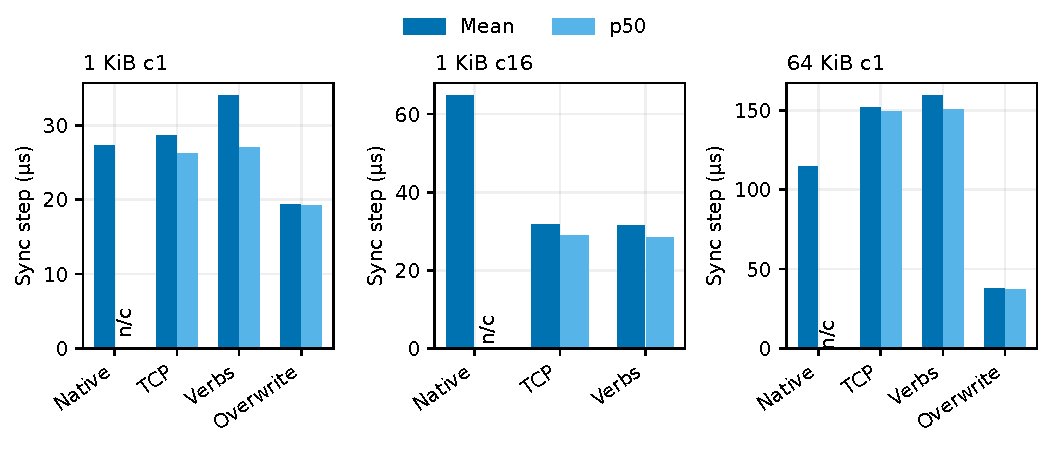
\includegraphics[width=.86\linewidth]{figures/sync-step.pdf}
\caption{Run 8, unified fleet, selected r0 (one repetition per point). Owner \texttt{wal\_file\_persist\_ns} times file fdatasync per retained record. Native \texttt{file\_ns + namespace\_ns} times file and directory fsync per API put. Native has means only. There is no c16 overwrite floor. The overwrite control is not an append baseline.}
\end{figure}
\begin{table}[H]\centering\fitinput{tab-sync.tex}
\caption{Run 8, unified fleet: in-process sync steps and overwrite controls, r0. Mean, p50 and p99 in \us; n/c means unavailable. Record counts differ at c16 because one owner sync can cover several puts. The 8 KiB overwrite row is context only.}
\end{table}
Compare mean to mean. At 1 KiB c1, owner TCP is \N{Y:t:1024:1:mean_us}~\us, owner verbs \N{Y:v:1024:1:mean_us}~\us, and native file-plus-directory \N{Y:n:1024:1:mean_us}~\us. The owner verbs mean carries a tail: p99 \N{Y:v:1024:1:p99_us}~\us. ``Equal at 1 KiB'' means within the owner tail, not identical means or distributions. Native has no sync-step p50 or p99. At 64 KiB, mean TCP \N{Y:t:65536:1:mean_us} and verbs \N{Y:v:65536:1:mean_us}~\us\ exceed native \N{Y:n:65536:1:mean_us}~\us. The owner gap is uniform on all five owners; its cause is open. At c16 one owner sync covers several puts; retained-record means are not per-put means.
These are the same kind of timed step, not the same system call: owners use one file fdatasync; Native uses fsync on every registered Value-WAL file, then opens and fsyncs the directory.

\subsection{Append floors: run-9 evidence}
\RWCFINDING{append} The four reviewed modes are overwrite fdatasync, append pwrite/fdatasync, append mmap/fdatasync and append mmap/fsync at 1/8/64 KiB, r0/r1. Fresh append offsets are written once (512 warmup, 4,096 measured operations). These controls were absent from run 8; their real receipts and representative means now appear in Appendix~\ref{app:rwc-floors}.

Match size and the same kind of durability call: mmap/fsync excludes Native directory fsync. \inference\ Similar or different client/owner floors motivate hardware/software hypotheses, not a measured software remainder. No separately sampled floor is subtracted from an API mean.

\clearpage
\section{Put stall}\label{sec:stall}
\begin{figure}[H]\centering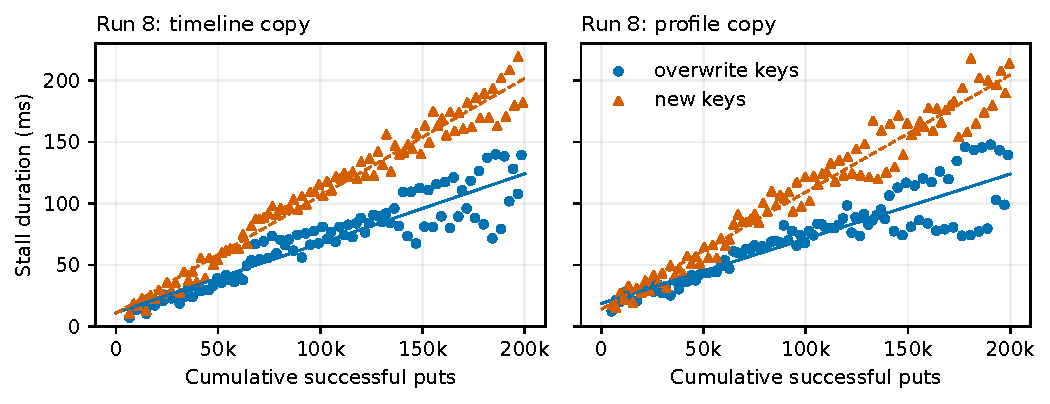
\includegraphics[width=\linewidth]{figures/put-stall.pdf}
\caption{Run 8, unified fleet: synchronous verbs 1 KiB c16, 200,000 puts. One repetition for each key policy and instrument. Dots are observed no-completion intervals; lines are fitted duration against cumulative successful puts. Both timeline and profile copies remain separate.}
\end{figure}
\begin{table}[H]\centering\fitinput{tab-stall.tex}
\caption{Run 8, unified fleet, one repetition per row. Fit $d(P)=a+bP$: $d$ and $a$ in \us, $P$ cumulative puts, $b$ in \us/put. Mean and median spacing are puts between stalls, extracted from raw \texttt{stall.csv} values. Queue and Prepare count the longest interval of linked following calls. n/c means the profile copy has no timeline.}
\end{table}
The timeline links only an initial subset of stalls. The longest linked intervals are owner enqueue to dequeue and prepared to admitted. They locate a queue, not the global stall cause. New keys have a steeper duration fit than overwrite. \inference\ Checkpoint work that grows with cumulative puts is a candidate. Neither this fit nor the phase count proves it. Instrument checkpoint work and correlate a call-linked trace before changing it.

\begin{table}[H]\centering\fitinput{tab-sustained.tex}
\caption{Separate fleet: run 7, focused device fleet, 1 KiB c16, 200,000 puts per case; three repetitions per route and tier shown separately. Successful puts/s: first complete one-second bucket, mean of the last five complete one-second buckets, whole case. Owner tier native means page-cache acknowledgement. No run-7/run-8 subtraction.}
\end{table}
The late rate falls below the first complete second in every repetition and both acknowledgement tiers. The corrected source excludes the final partial bucket. It supports a finite-case decline, not steady-state capacity or a stall cause. The earlier brief was biased low by that partial bucket; the historical report's late-rate range is consistent with the corrected complete buckets.

\clearpage
\section{Remote actions served by the SSD: run 7}\label{sec:run7}
\begin{figure}[H]\centering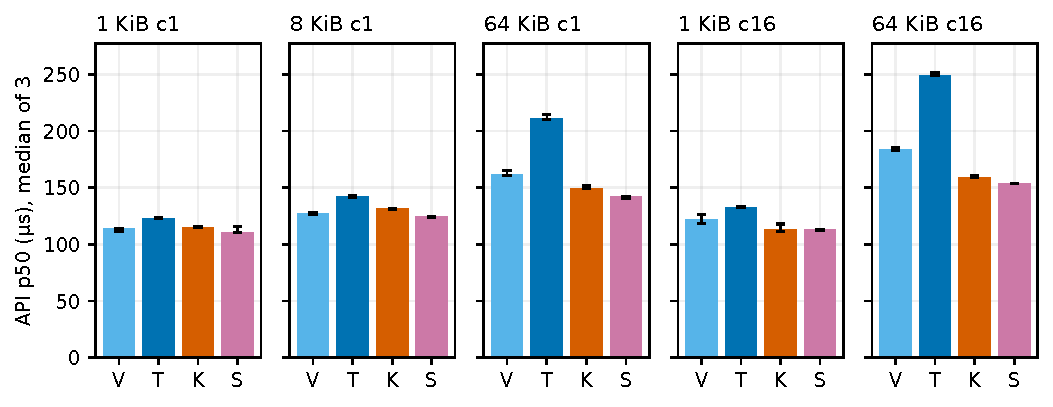
\includegraphics[width=\linewidth]{figures/run7-reads.pdf}
\caption{\rSeven. SSD-served reads, random keys with replacement. Median API p50 of three repetitions; whiskers show min to max, not a confidence interval. V: owner verbs trusted; T: owner TCP mTLS; K: kernel direct; S: SPDK. Target and initiator use direct I/O in K and S.}
\end{figure}
\begin{table}[H]\centering\fitinput{tab-run7-reads.tex}
\caption{Run 7, focused device fleet. API p50 in \us, median of three with min--max. Device reads/call is the median kernel-counter ratio. Owner 1 KiB cases retain a small page-cache-hit minority. Counts are 2,048 calls at 1 KiB and 4,096 at other sizes per repetition, over 65,536 keys.}
\end{table}
All run-7 read cases qualify. Authority history loads stay unchanged, so this does not cover history-load misses. The SPDK kernel-counter excess is a per-case constant, not a per-call device cost; its bdev layer reports one aligned read per call. Its origin is open. Direct I/O does not attest NAND access. Run-9 qualifications are separate (Appendix~\ref{app:rwc-qualification}).

\textbf{Sweep correction.} An ascending key sweep can let readahead or device buffering serve several values with one device read. Earlier sweep values must not be used as SSD-served random-read latency. Run 7 uses random keys with replacement. It replaces that interpretation, not the recorded earlier API measurements.

\clearpage
\subsection{Run 7 puts and durability cost}
\begin{figure}[H]\centering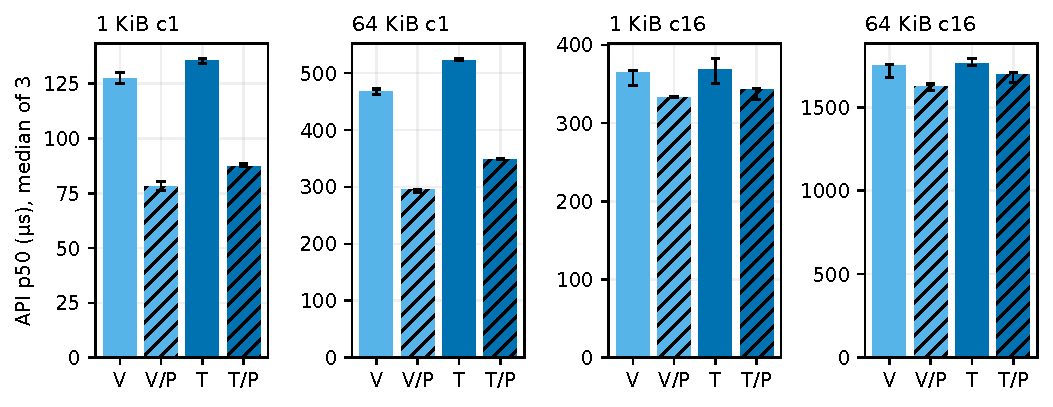
\includegraphics[width=\linewidth]{figures/run7-puts.pdf}
\caption{\rSeven. Owner puts: median API p50 over three repetitions, min--max whiskers. V: verbs trusted; T: TCP mTLS. Solid bars use synchronous acknowledgement; /P and hatched bars use the owner native (page-cache) tier. Hybrid has the same owner-verbs write path but was not separately measured here.}
\end{figure}
\begin{table}[H]\centering\fitinput{tab-run7-puts.tex}
\caption{Run 7, focused device fleet. Three repetitions, 4,096 successful puts each. API p50 in \us, median [min--max]. Synchronous waits for covering persistence. Page-cache tier does not.}
\end{table}
The acknowledgement-contract difference includes waiting for persistence, software and scheduling, not an isolated fsync timer. For owner verbs c1, the difference of median p50 values is about \N{E:run7_put1_gap|.0f}~\us\ at 1 KiB and \N{E:run7_put64_gap|.0f}~\us\ at 64 KiB. These descriptive differences compare separate populations on the same fleet. They are not additive components; run 8's in-process sync-step table measures the call directly. \path{run7-put_durability_ratio.csv} keeps matched repetition case ids and ratios.

The TCP-verbs difference includes mTLS. Three repetitions give an observed spread, not a significance claim. Do not combine run-7 unprofiled calls with run-8 profiles to claim profiling overhead or a performance change: the fleets differ. Hybrid direct arms gain relative to the owner paths with larger values and c16; their cache contracts remain explicit.

\clearpage
\section{Distributed against original engine, page-cache acknowledgement, one owner}\label{sec:contract-a}
\textbf{Class P (retained Class A): same-fleet puts.} Leased live NVMe-oF/RDMA
uses \texttt{wal\_replay}, lease-ahead and interrupt-driven writes. Native uses
\texttt{page\_cache}, not its stronger barrier. Each has one data SSD: Native
on the coordinator, distributed WAL on the remote owner. Only the remote arm
pays coordinator/index/network costs.

Combined run: revision \texttt{e0af084}, fleet \texttt{bench-e3638332bc2b43a1},
12 November; \N{B:contract-values:combined-cases:value|,.0f} cases,
\N{B:contract-values:combined-measured_calls:value|,.0f} measured calls.
Run 13: \texttt{3d5c0f7}, fleet \texttt{bench-c1dce8770c684804}, 12 November,
\N{B:contract-values:run13-compared_cells:value|,.0f} cases.
One owner and fleet per run, one or two repetitions per cell; short cases
except sustained puts. Only same-fleet Native partners enter the table.

\begin{table}[H]\centering\fitinput{tab-contract-a.tex}
\caption{Class P (retained Class A): page-cache acknowledgement on both sides.
Matched fleet, size, callers and repetition; API p50/p99/p99.9 in \us.
One Native process/SSD versus one remote owner/SSD; coordinator cache off.
Unprofiled leased \texttt{wal\_replay}, lease-ahead, no write polling.
Sources: each run's \texttt{puts.csv}; exact cases/columns in \texttt{contract-values.csv}.}
\end{table}

\textbf{Sustained P, no Native pair.} Combined run, 200,000 puts, 1 KiB,
sixteen callers: p50/p99/p99.9
\N{B:contract-values:sustained-p50_us:value|.1f}/\N{B:contract-values:sustained-p99_us:value|.1f}/\N{B:contract-values:sustained-p999_us:value|.1f}~\us;
\N{B:contract-values:sustained-calls_per_second:value|,.0f} puts/s at
\N{B:contract-values:sustained-mean_inflight_calls:value|.1f} mean in-flight calls;
\N{B:contract-values:sustained-calls_ge_5ms:value|,.0f} calls at least 5 ms.
Finite-case rates are not production capacity.

\textbf{First put, cross-fleet context only.} The unprofiled 1 KiB single-caller
first call changed from \N{B:contract-values:first-run13_first_call_us:value|.1f}
to \N{B:contract-values:first-first_call_us:value|.1f}~\us.
The regression fixture confirms removal of the measurement gate's warm-extent
close, not a controlled fleet timing A/B. Later large-value slow calls remain
unattributed. No hardware crash or power-loss test follows.
\subsection{Why the large-value put gap remains}\label{sec:contract-stages}
\textbf{Measured Class P (retained Class A), one owner.} Combined-run timeline
case \texttt{G20W-r0-fb6fb99bf8a683e8fbf4}: leased NVMe-oF, \texttt{wal\_replay},
lease-ahead, 64 KiB and \N{B:contract-values:stage-callers:value|.0f} callers.
The table averages consecutive coordinator event differences over all
\N{B:contract-values:stage-samples:value|,.0f} complete calls, not groups.

\begin{table}[H]\centering\fitinput{tab-contract-stages.tex}
\caption{Class P, one owner. Consecutive \texttt{timeline.records[].events}
\texttt{elapsed\_ns} differences, averaged over all complete calls.
Shares and residual use unrounded values; displayed sums can differ by rounding.
Same-clock intervals, not isolated wire or SSD time.}
\end{table}

I/O: \N{B:contract-values:stage-io_samples:value|.0f} timed writes including
\N{B:contract-values:stage-skip_markers:value|.0f} skip markers;
\N{B:contract-values:stage-groups:value|.0f} data groups,
\N{B:contract-values:stage-puts_per_group:value|.1f} puts/group,
\N{B:contract-values:stage-group_period_ms:value|.2f} ms/group,
\N{B:contract-values:stage-group_mib:value|.2f} MiB/group including framing.
Span (last completion minus first scheduled call) gives \N{B:contract-values:stage-leased_mib_s:value|.0f} MiB/s
of framed WAL traffic (\N{B:contract-values:stage-payload_mib_s:value|.0f} MiB/s
of logical payload). Summed leased-write time gives
\N{B:contract-values:stage-mean_leased_write_ms:value|.2f} ms per I/O sample,
\N{B:contract-values:stage-active_write_gib_s:value|.2f} GiB/s while writing,
and \N{B:contract-values:stage-write_busy_pct:value|.1f}\% of the measurement span.
These are counter-derived intervals, not device-only service times.

\inference\ The device and network are not the limit indicated by this case.
Preparation runs on one \texttt{wal-write-owner} coordinator thread
(\path{remote_db/concurrent.rs:455}); at the observed mean,
\N{B:contract-values:stage-callers:value|.0f} preparations take about
\N{B:contract-values:stage-serial_preparation_ms:value|.2f} ms per group.
The two large waits may queue behind that thread and one in-flight group.
Five owners spread only the write stage
(\N{B:contract-values:stage-live_io_share:value|.1f}\% of call time), not preparation:
inference until Run B. Sources and formulas: \texttt{contract-stage-metrics.json}
and the README.

\clearpage
\subsection{Separate Class B controls and read-path context}\label{sec:contract-b-controls}
These controls are not Class A put comparisons. Run 13 measured the new
\texttt{wal\_replay} design with synchronous-tier puts at one caller only.
The read rows also record Class B preparation: their CSV contract is
\texttt{durable}. They must not be relabelled as page-cache-acknowledged
experiments. Live reads use a buffered target: warm after prewarm, cold
after eviction with case-level device qualification (run-13 \texttt{settings.csv}). Native
memory reads and Valkey RAM reads are not cold-device controls.

\begin{table}[H]\centering\fitinput{tab-contract-b-controls.tex}
\caption{Separate Class B settings: synced-before-acknowledgement puts;
read rows name the write/preparation setting, not a read durability guarantee.
Run 13 only, one owner, one repetition per row, coordinator cache off.
The leased put uses lease-ahead; owner RPC is a different route. Polled warm
read is a separate arm. API quantiles are \us, not device-service times.
Sources: run-13 \texttt{puts.csv} and \texttt{reads.csv}; no subtraction or
cross-class ranking.}
\end{table}

The combined fleet's only read cell is a cold live read with a synchronous
(Class B) setup. It is not a Class A Native-read partner. Run 13's requested
cold Native small-value read failed device qualification; its memory-like
p50 cannot supply a cold comparison. The indicative table below keeps the
new read path separate from Valkey's RAM GET.

\textbf{Open items.} No Sui replay result on hardware; no new synchronous-tier
put measurement at sixteen callers; no five-owner run with this design;
no Class A external-store measurement. The failed Sui producer did not
reach either measured replay, so it supplies no timing, digest comparison
or state audit on hardware. The earlier ranked decisions are historical
hypotheses, not evidence that these gaps are closed.

\subsection{Order of magnitude only: new one-owner NVMe-oF design against historical Valkey RDMA}\label{sec:indicative}
\textbf{Indicative only. No ranking follows.} API p50 in \us; semicolons keep
new repetitions separate. Read labels state memory or device service.
Valkey cells retain the historical per-run-p50 median for RAM GET.

\begin{table}[H]\centering\fitinput{tab-contract-indicative.tex}
\caption{Order of magnitude only, not an equal-contract comparison.
Owner count: one Tidehunter owner versus five Valkey storage nodes.
Contract: new puts are Class A page-cache acknowledgement; Valkey SET is
Class B \texttt{appendfsync always}; new read rows have Class B setup but
Valkey reads come from RAM; new reads label memory or device service. Fleet: combined
or run 13 versus historical external fleets, never the same fleet.
Date: new cloud fleets created 12 November 2026; historical contributors
span earlier November fleets (per-run dates in \texttt{historical-topology.csv}).
Workload profile: new puts/read-only cells versus Valkey mixed point calls
at one caller and pure write/read-concurrent cells at sixteen callers;
new repetitions are individual runs, Valkey is a historical median.
These differences prevent any ranking. ``Not measured'' is not zero;
no value is interpolated. Sources: new-run \texttt{puts.csv}/\texttt{reads.csv}
and historical \texttt{populations.csv}, column \texttt{api\_p50\_us}.}
\end{table}


\clearpage
\section{Cross-store comparison: carried forward}\label{sec:cross}
\textbf{\carried.} Native and Tidehunter use fleet \texttt{bench-0d99e8256fff4891}, six \texttt{z4m-highmem-16} VMs in \texttt{us-central1-a}, RDMA and Local SSD. External-store statistics span other GCP fleets, days and binaries. These are not run-7, run-8 or run-9 measurements. Coordinator cache is off. API quantiles are success-only. Native waits for its own per-put Value-WAL file and directory fsync; owner synchronous waits for a covering fdatasync, which can serve several puts. Valkey uses AOF \texttt{appendfsync=always}. Similar durable intent does not prove equal persistence mechanics.

\subsection{Topology, contracts and the Native result}\label{sec:native-gap}
The reading guide below applies only to the retained full-matrix figures, not the compact run-9 topology.
\textbf{How to read these figures.} Native: one process, one SSD. Tidehunter: five owners. Other external contributors record five configured or observed storage nodes; Cassandra's 3 November run records five contacts, not a verified five-node ring. Five storage-host SSD mounts are attested only for the inspected 4 November and final deployments. FoundationDB also has a separate log/coordinator host. Equal RF1 is not equal SSD count. Native performs file and directory fsync after each put; owner covering fdatasync can serve multiple batches. Valkey waits for AOF fsync once per event-loop pass\footnote{Valkey 9.0.7, \texttt{src/server.c}: \texttt{beforeSleep} flushes AOF before pending client writes. See \url{https://github.com/valkey-io/valkey/blob/9.0.7/src/server.c} and \url{https://valkey.io/topics/persistence/}. Commands per sync were not measured in these runs.}; Kvrocks uses a synced RocksDB WAL; Garnet waits for AOF commit. Hollow write markers mean Cassandra, FoundationDB and TiKV device persistence is not verified. \runs. Hardware and configuration are not fully matched.

API time is completion minus dispatch; response time is completion minus schedule time, before dispatch and admission. Both use successful calls. Valkey reads RAM; Native uses a resident-oriented read workload, with per-call source not established; owner and hybrid cache paths differ. In the two c16 read figures, panel four is mean in-flight successful API calls: each run's sum of successful API times divided by elapsed case time, then the median across external runs. In the two c1 figures, it is the selected operation's API mean. Low occupancy means that finite rates do not establish store capacity. Both axes are logarithmic; x-axis K means binary bytes, while y-axis k and M are decimal.
\textbf{Topology and durable mechanics.} Native is one process on one SSD; the retained final cases of other systems use five storage nodes. Native's retained per-put benchmark barrier calls \texttt{Db::insert}, then fsyncs every registered Value-WAL file and opens and fsyncs the directory after each put. That arm does not group scalar callers; the separate run-9 grouped Native arm does. Owner synchronous acknowledges after its covering file fdatasync; batches appended during one sync can share the next sync. A missing network hop does not make Native a latency lower bound under another contract or topology. These settings express durable intent, not proved crash or device-persistence equivalence.

\begin{table}[H]\centering\fitinput{tab-per-node.tex}
\caption{64 KiB puts, c16: aggregate rate / retained-final node count. Even spread assumed for callers, rate and payload; these are normalizations, not observed node-level metrics. Native: one process, one SSD. Tidehunter: five owners. Other external contributors record five configured or observed storage nodes; Cassandra's 3 November run records five contacts, not a verified five-node ring. Five storage-host SSD mounts are attested only for the inspected 4 November and final deployments. FoundationDB excludes its separate log/coordinator host. Rates use finite case time, including work outside API calls. Native: per-put file/directory barrier; TH: covering sync; Valkey: AOF-always; Garnet: AOF commit; Kvrocks: synced WAL. Other writes have unverified device persistence. No cache drop; coordinator cache off. \runs. c1 is mixed, not pure-write.}\label{tab:pernode}
\end{table}
Final counts come from case configs and observed topology, recorded in \path{storage-topology.csv}. Other external contributors record five configured or observed storage nodes; Cassandra's 3 November run records five contacts, not a verified five-node ring (\path{historical-topology.csv}). This is not verification from every case configuration or proof of five physical SSDs. Five storage-host SSD mounts are attested only for the inspected 4 November and final deployments. FoundationDB excludes its separate log/coordinator host; TiKV excludes PD. Some 3 November FoundationDB machine ids and TiKV host labels name a different fleet from the report path; the path does not establish execution-fleet identity.

The gate-window completed-write counts span \N{B:device-write-spread:th_verbs:minimum|,.0f}--\N{B:device-write-spread:th_verbs:maximum|,.0f} across owner verbs nodes (max/min \N{B:device-write-spread:th_verbs:ratio|.2f}) and \N{B:device-write-spread:valkey_rdma:minimum|,.0f}--\N{B:device-write-spread:valkey_rdma:maximum|,.0f} across Valkey RDMA primaries (\N{B:device-write-spread:valkey_rdma:ratio|.2f}). These final-run counters include background work and use different node windows; they are not API-linked rates or the historical median case.

\textbf{The Native observation.} At 64 KiB, barrier c16 p50/mean are \N{B:per-node-64k:native:p50_us}/\N{B:per-node-64k:native:mean_us}~\us, with \N{B:per-node-64k:native:puts_s|,.0f} puts/s and \N{B:per-node-64k:native:mean_inflight_calls} in-flight calls. Mixed c1 barrier p50/mean are \N{p50:native:primary_rf1:point-mixed:put:65536|.1f}/\N{mean:native:primary_rf1:point-mixed:put:65536|.1f}~\us. The mean ratio is \N{J:native_mean_ratio}; the reciprocal c1 API mean is \N{J:native_reciprocal|,.0f} puts/s, not measured c1 throughput, and c16 reaches \N{J:native_reciprocal_pct|.0f} percent of that reference. \inference\ The illustration assumes that mixed-stream c1 API service represents pure-write service; the workloads differ, so the ratios do not demonstrate serialization. A serialized-service model with one independent barrier per put is consistent with the ratios, but API calls overlap; no trace separates sync serialization, queue depth, faults, allocation or journal work.

Native page-cache acknowledgement has no per-put foreground fsync or per-put persistence guarantee. Its 64 KiB c16 p50 is \N{J:pagecache64}~\us\ and mixed c1 p50 is \N{J:pagecache_c1_64}~\us. Its c16 p50 is \N{J:pagecache_jump} times the 8 KiB value of \N{J:pagecache8}~\us. The cause is not established. \inference\ Faults, allocation, writeback and fragment events are candidates, not measured contributions. The rate panel omits this page-cache series: its API occupancy is low through 8 KiB but higher at 64 KiB. Owner page-cache write curves were not run on this fleet and are not drawn.

\textbf{Where Valkey is ahead, and where it is not.} The c1 mixed-stream readings and c16 figures show different populations, not a controlled concurrency sweep. At 1 KiB, owner synchronous verbs is ahead of historical Valkey RDMA AOF-always on c1 put p50; owner resident-oriented reads are also ahead of Valkey RAM GET at c1. At c16, the 1 KiB read p50 values are close (owner \N{p50:th_verbs:primary_rf1:read-concurrent:read:1024|.1f}~\us; Valkey \N{p50:valkey_rdma:primary_rf1:read-concurrent:read:1024|.1f}~\us). Valkey is ahead on c16 put p50 at 1 and 64 KiB, and c1 mixed put at 64 KiB; owner read p50 is ahead at 64 KiB for c1 and c16. This is not a claim that every store wins at every size or quantile: Garnet's commit-wait c16 put p99 at 1 KiB is \N{p99ms:garnet:primary_rf1:write-concurrent:put:1024|.1f}~ms; the stall cause is not established.

At 64 KiB c16, the even-spread rate is \N{B:per-node-64k:valkey_rdma:puts_s_node|,.0f} puts/s/node for Valkey RDMA AOF-always, \N{B:per-node-64k:th_verbs:puts_s_node|,.0f} for owner synchronous verbs, and \N{B:per-node-64k:native:puts_s_node|,.0f} for the one-SSD Native barrier. Group commit is possible in Valkey and the owner; actual commands per sync are not measured. The aggregate rate alone cannot identify batch size, sync time or the cause of their difference.

\inference\ Waits, hand-offs and size-dependent software are plausible owner limits, not proof that the SSD has no role. On the separate run-8 fleet, synchronous verbs c16 1 KiB has \N{W:p16v|.0f} percent of its same-case API mean in three waits (\N{C:p16v:coalescing}, \N{C:p16v:queue}, \N{C:p16v:durable} of \N{D:p16v:mean_us}~\us). At c1 64 KiB, coordinator plus owner software is \N{J:owner64_software_pct|.0f} percent (\N{C:p64v:coordinator} plus \N{C:p64v:owner} of \N{D:p64v:mean_us}~\us). These intervals are not avoidable-cost bounds and must not be subtracted from separately sampled Valkey measurements.

\textbf{Fleet and profile context.} Run-8 unprofiled c1 1 KiB synchronous verbs put p50/mean is \N{D:uput1v:p50_us}/\N{D:uput1v:mean_us}~\us; the full-matrix mixed point put is \N{p50:th_verbs:primary_rf1:point-mixed:put:1024|.1f}/\N{mean:th_verbs:primary_rf1:point-mixed:put:1024|.1f}~\us. They differ in fleet, workload and repetition count. This difference is not a measured regression or profiling cost. Run 8 also compares one Native SSD with five owners; its c16 64 KiB Native barrier is not an equal-device-count control.
The compact one-owner control in Section~\ref{sec:rwc} is a distinct run, not a before/after regression test or a replacement for these five-owner populations.

\textbf{Unexplained features.} Garnet AOF-commit c16 put p99 stays near \N{p99ms:garnet:primary_rf1:write-concurrent:put:1024|.1f}--\N{p99ms:garnet:primary_rf1:write-concurrent:put:256|.1f}~ms across sizes; retained 64 B samples show stalls of about \N{B:chart-anomalies:garnet:stall_min_ms|.0f}--\N{B:chart-anomalies:garnet:stall_max_ms|.0f}~ms. FoundationDB p50 plateaus near \N{p50:foundationdb:primary_rf1:write-concurrent:put:64|.0f}~\us, then dips to \N{p50:foundationdb:primary_rf1:write-concurrent:put:8192|.0f}~\us\ at 8 KiB; Cassandra steps from \N{p50:cassandra:primary_rf1:write-concurrent:put:256|.0f} to \N{p50:cassandra:primary_rf1:write-concurrent:put:1024|.0f}~\us\ between 256 B and 1 KiB. Both have unverified device persistence. Native barrier p50 dips from \N{p50:native:primary_rf1:write-concurrent:put:256|.1f} to \N{p50:native:primary_rf1:write-concurrent:put:1024|.1f}~\us. Owner synchronous kernel/SPDK put curves lie above TCP/verbs. No cause is claimed. See \path{external-spread.csv} for external per-run spread; no whiskers are drawn.


\clearpage
\textbf{The retained pre-run-9 64 KiB points are reproducible.} The retained c16 cases reproduce the high Native latency, not a particular cause. Table~\ref{tab:spike} shows each population separately. Native per-put barrier p50 spans \N{B:spike-summary:B_minimum:value|,.1f}--\N{B:spike-summary:B_maximum:value|,.1f}~\us; Native page-cache p50 spans \N{B:spike-summary:P_minimum:value|.1f}--\N{B:spike-summary:P_maximum:value|.1f}~\us. These are observed ranges, not confidence intervals or sustained-capacity results. Run-9 grouped-barrier controls are separate, not additions to these historical ranges.

\begin{table}[H]\centering\fitinput{tab-spike.tex}
\caption{Individual 64 KiB c16 successful-put API p50 values, recomputed from raw samples; \N{B:spike-cases:M_0379-native-65536-write-concurrent-primary_rf1-r0:n|,.0f} puts per population. B: Native per-put all-file/directory barrier, one process/SSD. P: Native page-cache acknowledgement, no per-put foreground fsync or per-put persistence guarantee. S: owner verbs synchronous covering persistence, five owners. V: Valkey RDMA AOF-always. Cache state is not controlled; coordinator cache is off in the distributed KV cases. N3: 3 November campaign; M: full matrix; R7/R8: focused fleets. R8 K/N/W are different profiles, not extra independent repetitions; columns retain each profile's repetition index. O/D: 4 November manual read/delete exports; Q: queue campaign. Copied baselines in manual exports are not proved independent fleets. Full case ids, sample/archive paths and contracts are in \texttt{spike-cases.csv}. No populations are pooled.}\label{tab:spike}
\end{table}

The full-matrix Native barrier distribution has p10/p50/p99 \N{B:spike-cases:M_0379-native-65536-write-concurrent-primary_rf1-r0:p10_us|,.1f}/\N{B:spike-cases:M_0379-native-65536-write-concurrent-primary_rf1-r0:p50_us|,.1f}/\N{B:spike-cases:M_0379-native-65536-write-concurrent-primary_rf1-r0:p99_us|,.1f}~\us. Only \N{B:spike-cases:M_0379-native-65536-write-concurrent-primary_rf1-r0:above_twice_pct|.2f} percent exceed twice its median. Its equal-count, dispatch-ordered quarter medians are \N{B:spike-cases:M_0379-native-65536-write-concurrent-primary_rf1-r0:q1_p50_us|,.1f}, \N{B:spike-cases:M_0379-native-65536-write-concurrent-primary_rf1-r0:q2_p50_us|,.1f}, \N{B:spike-cases:M_0379-native-65536-write-concurrent-primary_rf1-r0:q3_p50_us|,.1f} and \N{B:spike-cases:M_0379-native-65536-write-concurrent-primary_rf1-r0:q4_p50_us|,.1f}~\us. The main body is slow, not only a few outliers; the quarters show no monotonic warm-up decline.

The full-matrix page-cache case also has a slow main body: p10/p50/p99 \N{B:spike-cases:M_0490-native-65536-write-concurrent-native_async_write-r0:p10_us|.1f}/\N{B:spike-cases:M_0490-native-65536-write-concurrent-native_async_write-r0:p50_us|.1f}/\N{B:spike-cases:M_0490-native-65536-write-concurrent-native_async_write-r0:p99_us|.1f}~\us. Its last quarter is slower than its first; this does not identify a cause.

The following one-barrier-per-put policy describes the retained Native per-put arm, not the separate run-9 grouped Native barrier.
The barrier policy is known: one library barrier after every put, without an application-level covering group. \inference\ The serialized-service model is consistent with the earlier c1/c16 ratios, but kernel sync work can overlap. The page-cache jump from 8 to 64 KiB remains unexplained: \N{J:pagecache_jump} times the p50 for eight times the payload. Worker identity and per-put WAL offsets are absent from \path{samples.csv}; fragment-boundary clustering cannot be tested. The API clock includes engine frame encoding, CRC and WAL copying, but excludes harness value generation and oracle bookkeeping. Sources: \path{runner.rs:2655--2808}, \path{backends/native.rs:173--179,295--300}, \path{db.rs:579--594,2157--2167} and \path{crc.rs:17--29}; paths are relative to the benchmark or engine source directories.

\clearpage
\textbf{Local structure test (laptop, not the cloud).} This later audit used IEEE CRC32, which matches the engine's checksum polynomial, not its full implementation. The machine ran kernel \texttt{7.2.6}, ext4 on local NVMe, not cloud Local SSD. The local c16 slowdown appears at 8 KiB as well as 64 KiB; it does not reproduce the cloud's size-specific page-cache jump. \inference\ Write-prefault and \texttt{pwrite} still slow down under concurrency, so neither page faults nor copy contention is rejected. The grouped ticket model was not uniformly faster: its 64 KiB c16 p50 was \N{B:local-structure-test:grouped_data_sync_64_c16_r1:p50_ms|.2f}/\N{B:local-structure-test:grouped_data_sync_64_c16_r2:p50_ms|.2f} ms in runs 1/2, against \N{B:local-structure-test:data_sync_64_c16_r1:p50_ms|.2f} ms for per-put data sync. It is not evidence for a grouped-barrier speedup. The cloud step's cause stays open.

\begin{table}[H]\centering\fitinput{tab-local-structure.tex}
\caption{Local structure test: transcribed from the audit report; raw samples not retained. Each cell lists IEEE run 1; run 2 separately; -- means not measured. Fresh mapping, \texttt{MAP\_POPULATE}, write-prefault, \texttt{pwrite} and anonymous memory have no per-put foreground persistence guarantee. Write-prefault writes every page and data-syncs before timing; \texttt{MAP\_POPULATE} is not that control. Data sync means per-put \texttt{fdatasync}; grouped sync is a covered-ticket model. Neither is the engine's complete file-and-directory barrier. Finite-case rates are not capacity estimates; per-call occupancy cannot be checked without retained samples. Source and run labels are in \texttt{local-structure-test.csv}.}\label{tab:local-structure}
\end{table}

\begin{minipage}{\linewidth}
\subsubsection{Fair Native comparison: compact subset measured}\label{sec:fair-native}
Run 9 measures the one-Db Native and one-owner TCP/verbs subset at equal total writers \N{B:fair-native-plan:G14N:writer0|.0f}, \N{B:fair-native-plan:G14N:writer1|.0f} and \N{B:fair-native-plan:G14N:writer2|.0f}. Native page-cache, per-put barrier and grouped barrier remain distinct from owner covering persistence (Section~\ref{sec:rwc}). The five-Db Native and five-owner rows below remain unmeasured design inventory; page-cache acknowledgement is not durable.

\begin{table}[H]\centering\fitinput{tab-fair-native.tex}
\caption{Frozen design inventory, not counts of completed run-9 cases. Run 9 includes G14N/G14O1 and three separate G14P diagnostics; G14S and G14O5 were not run. Instances, SSD location/count, network/security, sync scope and routing remain unmatched.}\label{tab:fair-native}
\end{table}

\texttt{fair\_native} has \N{B:fair-native-plan:fair_native:cases|.0f} designed cases; \texttt{parity} has \N{B:fair-native-plan:parity:cases|.0f}, including \N{B:fair-native-plan:G13W:cases|.0f} G13W floors. Run 9 executed the authorized \texttt{remote\_rw\_compact} subset, not either entire larger selection. Frozen digests in \texttt{fair-native-plan.csv} remain unchanged. A five-SSD Native arm remains unimplemented; further launches need separate approval.
\end{minipage}


\clearpage
\subsection{Cross-store curves}\label{sec:curves}
These five figures retain the historical full-matrix/external populations, not run-9 measurements. The new matched-caller grid is in Section~\ref{sec:rwc}.

\begin{figure}[H]\centering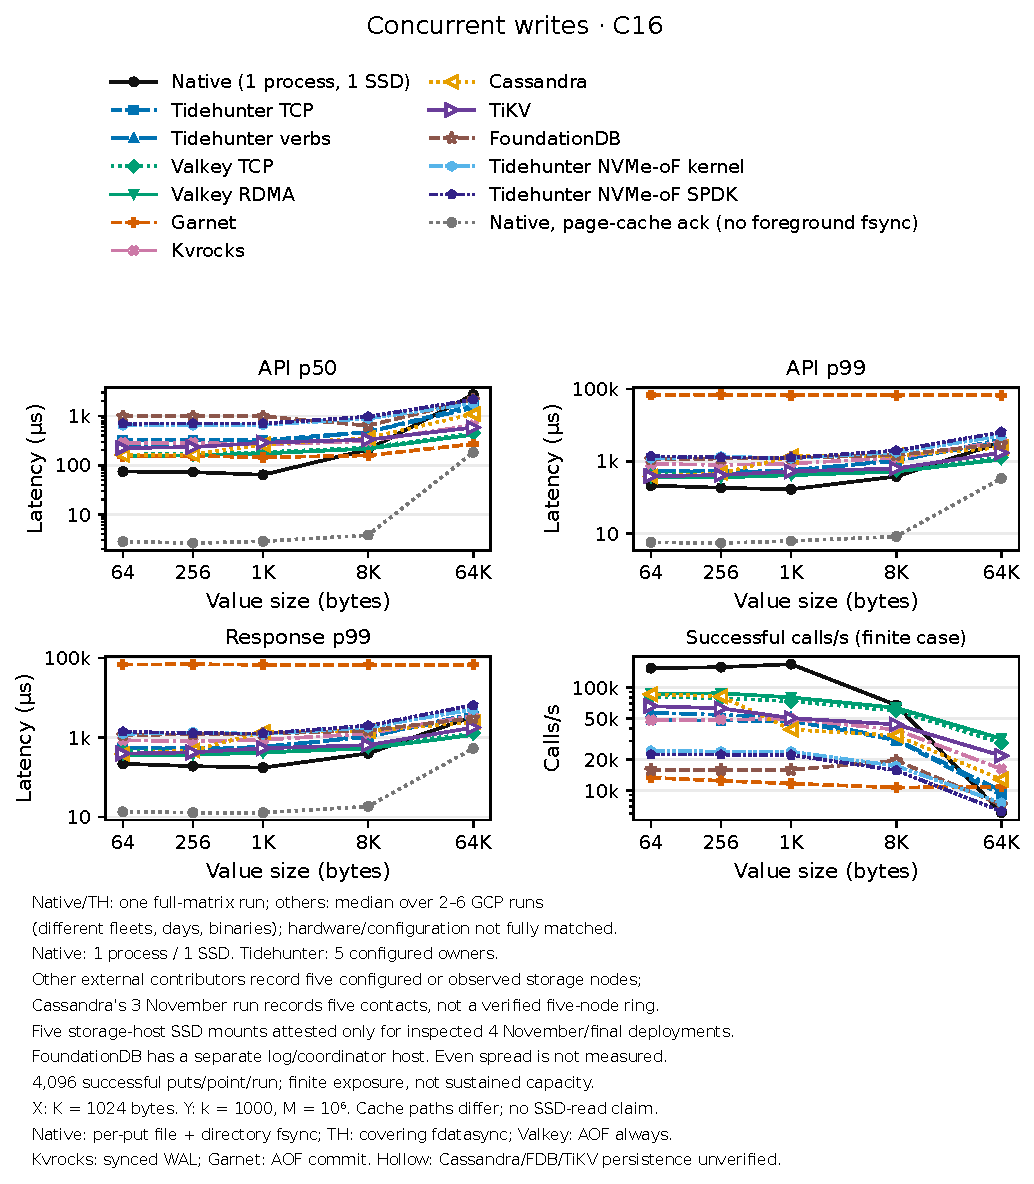
\includegraphics[width=\linewidth]{figures/curves-write-c16.pdf}
\caption{Verified series: Class B, synced before acknowledgement. \ackUnknown\ Separate grey Native Class A: \texttt{native\_async\_write}, page cache, no foreground fsync; finite rate omitted. Scalar puts, c16. Primary RF1; \N{curve:write-concurrent:put:calls} successful puts/run. \runs. Sync mechanics and topology differ; no cross-class ranking.}\label{fig:curves-write}
\end{figure}
At 1 KiB, synchronous verbs p50 is \N{p50:th_verbs:primary_rf1:write-concurrent:put:1024|.1f}~\us; historical Valkey RDMA AOF-always p50 is \N{p50:valkey_rdma:primary_rf1:write-concurrent:put:1024|.1f}~\us. At 64 KiB, Native's one-SSD per-put barrier has p50 \N{p50:native:primary_rf1:write-concurrent:put:65536|.1f}~\us; five-owner synchronous verbs has \N{p50:th_verbs:primary_rf1:write-concurrent:put:65536|.1f}~\us. Section~\ref{sec:native-gap} explains the topology and acknowledgement mismatch; the plot does not isolate their costs.

\clearpage
\begin{figure}[H]\centering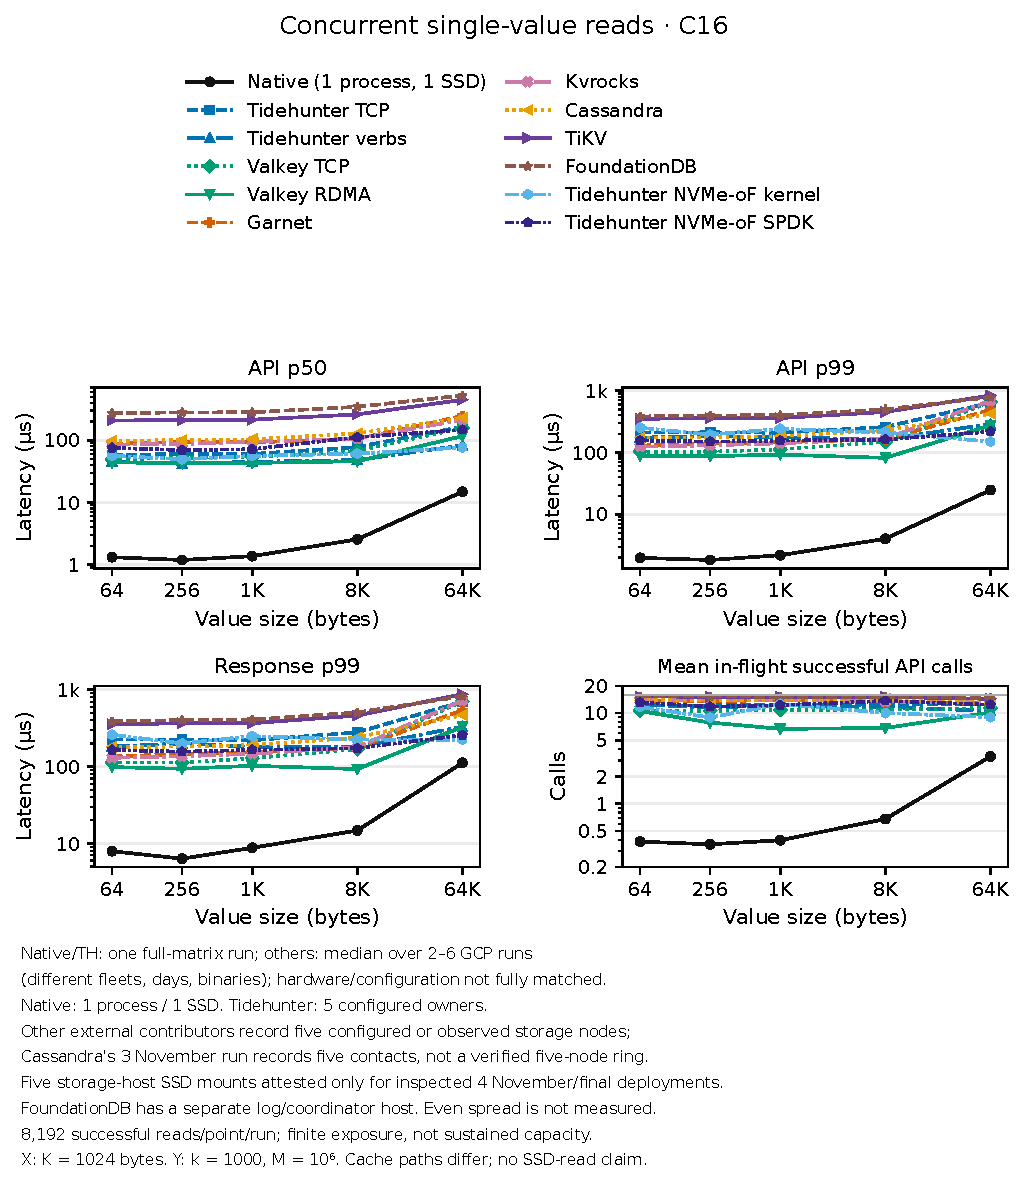
\includegraphics[width=\linewidth]{figures/curves-read-c16.pdf}
\caption{\ackB\ \ackUnknown\ Single-value reads, primary RF1, c16. Each point: \N{curve:read-concurrent:read:calls} successful reads/run. \runs. Panel four shows mean in-flight successful API calls per run, then the external median. The grey line marks 16 workers; it is not a store series. Cache paths differ; no SSD-latency ranking follows.}\label{fig:curves-read}
\end{figure}
At 64 KiB, owner verbs resident-oriented read p50 is \N{p50:th_verbs:primary_rf1:read-concurrent:read:65536|.1f}~\us, versus historical Valkey RDMA RAM GET \N{p50:valkey_rdma:primary_rf1:read-concurrent:read:65536|.1f}~\us. Native's resident-oriented p50 is \N{p50:native:primary_rf1:read-concurrent:read:65536|.1f}~\us; its low occupancy means its case rate is not a capacity estimate. Owner TCP includes mutual TLS; trusted verbs does not.

\clearpage
\begin{figure}[H]\centering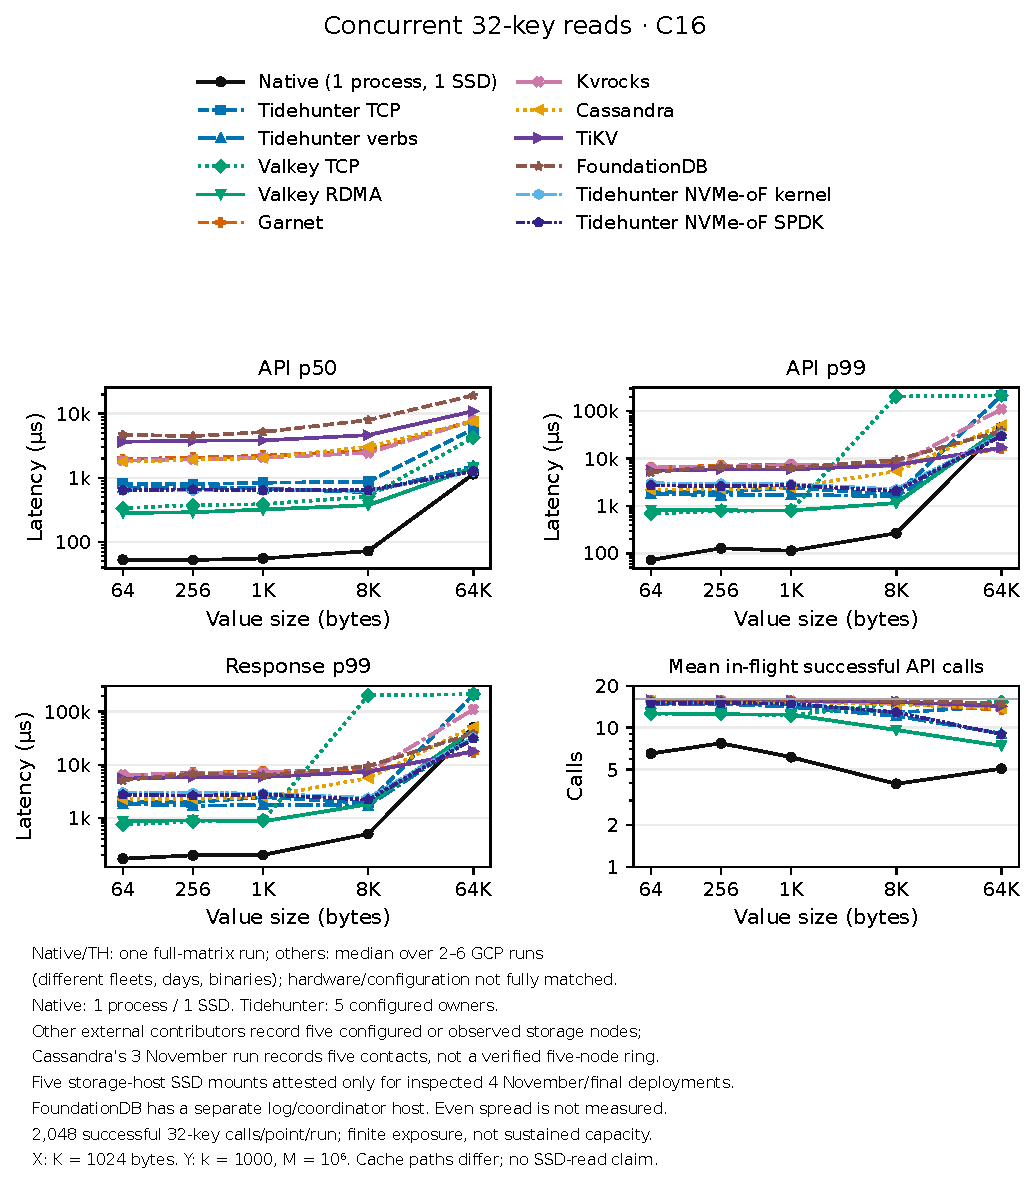
\includegraphics[width=\linewidth]{figures/curves-read32-c16.pdf}
\caption{\ackB\ \ackUnknown\ 32-key reads, primary RF1, c16. Each point: \N{curve:read-many32:get_many:calls} successful calls/run, each for 32 keys. \runs. Panel four shows mean in-flight successful API calls per run, then the external median. The grey line marks 16 workers; it is not a store series. It counts calls, not keys. Read caches differ.}\label{fig:curves-read32}
\end{figure}
At 1 KiB per value, owner verbs resident-oriented p50 is \N{p50:th_verbs:primary_rf1:read-many32:get_many:1024|.1f}~\us; historical Valkey RDMA RAM-read p50 is \N{p50:valkey_rdma:primary_rf1:read-many32:get_many:1024|.1f}~\us. At 64 KiB per value, verbs p99 is \N{p99ms:th_verbs:primary_rf1:read-many32:get_many:65536|.1f}~ms versus Valkey RDMA \N{p99ms:valkey_rdma:primary_rf1:read-many32:get_many:65536|.1f}~ms. Native uses one local SSD and a resident-oriented workload; these are not matched cold-device calls.

\clearpage
\begin{figure}[H]\centering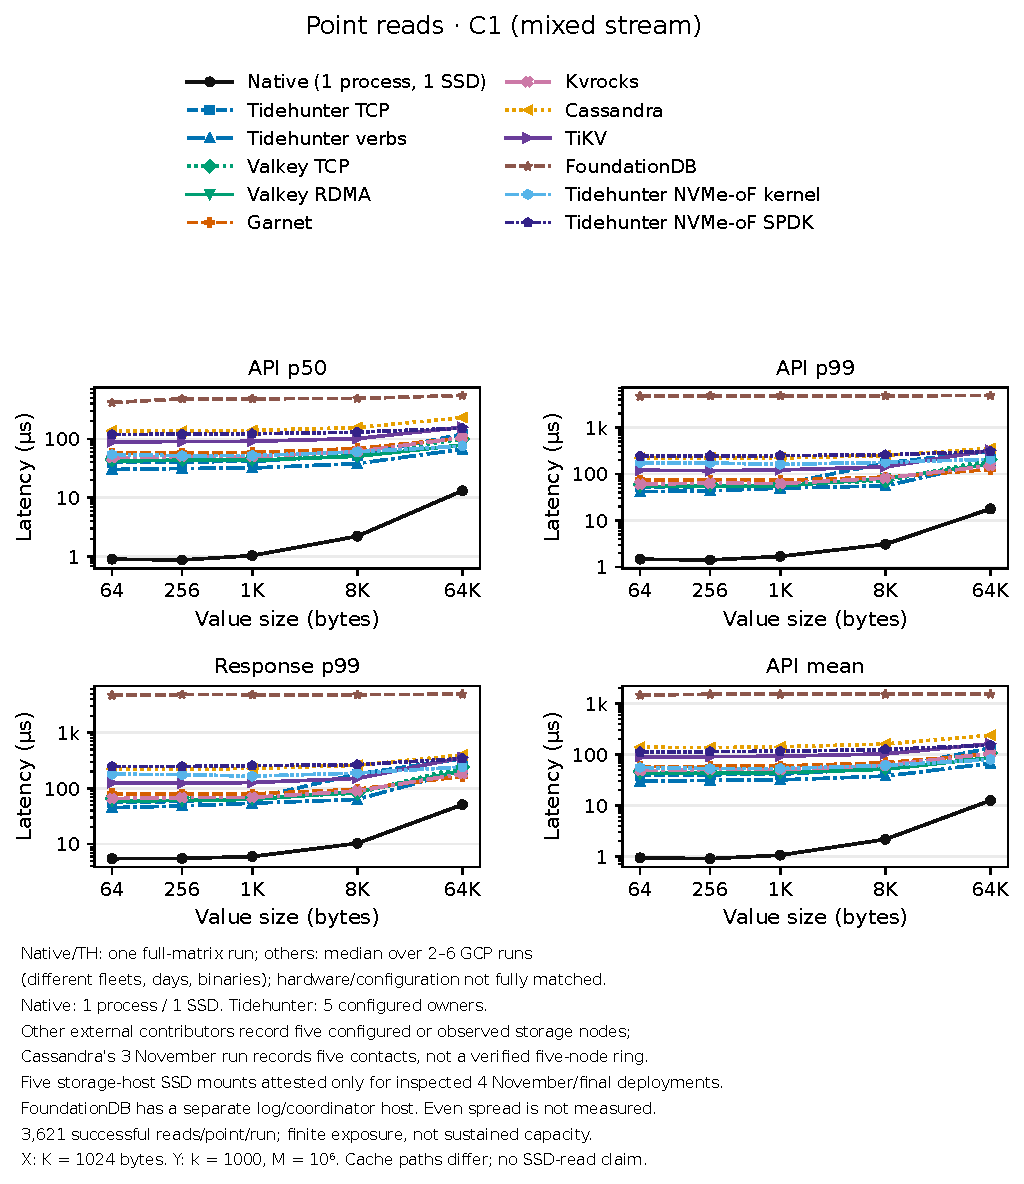
\includegraphics[width=\linewidth]{figures/curves-point-read-c1.pdf}
\caption{\ackB\ \ackUnknown\ Point reads at c1 within a mixed stream. Each latency point: \N{curve:point-mixed:read:calls} successful reads/run in a \N{curve:point-mixed:read:case_calls}-call case with puts, deletes and missing reads. \runs. Panel four shows read API mean, not mixed-case throughput. Cache paths differ.}\label{fig:curves-point-read}
\end{figure}
At 1 KiB, owner verbs resident-oriented p50 is \N{p50:th_verbs:primary_rf1:point-mixed:read:1024|.1f}~\us, versus historical Valkey RDMA RAM GET \N{p50:valkey_rdma:primary_rf1:point-mixed:read:1024|.1f}~\us. At 64 KiB, the corresponding p50 values are \N{p50:th_verbs:primary_rf1:point-mixed:read:65536|.1f} and \N{p50:valkey_rdma:primary_rf1:point-mixed:read:65536|.1f}~\us. This mixed stream is not the read-only c16 workload; it does not isolate concurrency scaling.

\clearpage
\begin{figure}[H]\centering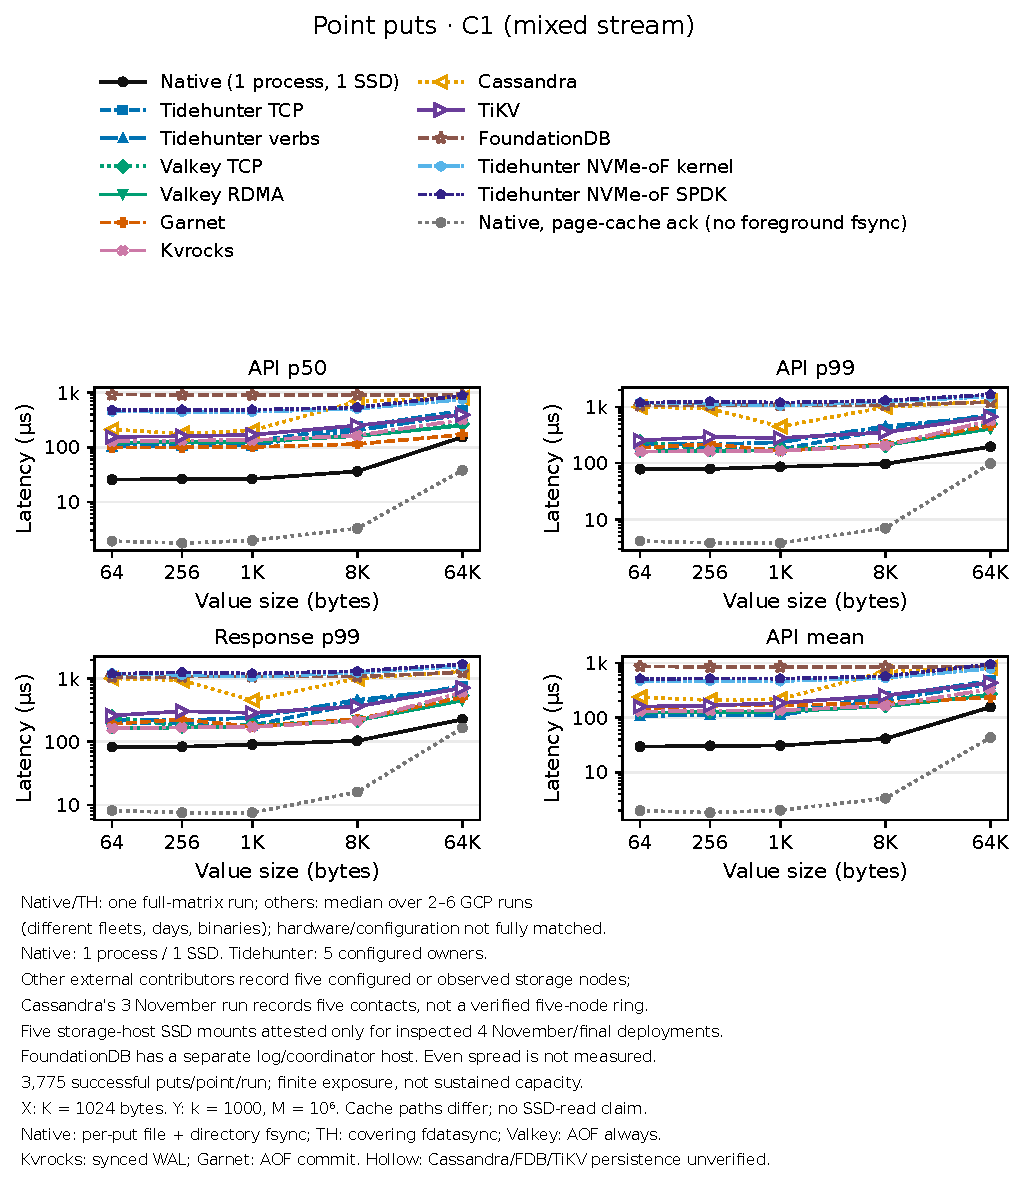
\includegraphics[width=\linewidth]{figures/curves-point-put-c1.pdf}
\caption{\ackB\ \ackUnknown\ Point puts at c1 within a mixed stream. Each latency point: \N{curve:point-mixed:put:calls} successful puts/run in a \N{curve:point-mixed:put:case_calls}-call case. \runs. Panel four shows put API mean. Grey dotted Native is a separate Class A page-cache reference; it has no per-put foreground fsync or per-put persistence guarantee; hollow markers mean unverified device persistence.}\label{fig:curves-point-put}
\end{figure}
At 1 KiB, owner synchronous verbs p50 is \N{p50:th_verbs:primary_rf1:point-mixed:put:1024|.1f}~\us; historical Valkey RDMA AOF-always p50 is \N{p50:valkey_rdma:primary_rf1:point-mixed:put:1024|.1f}~\us. At 64 KiB, those values are \N{p50:th_verbs:primary_rf1:point-mixed:put:65536|.1f} and \N{p50:valkey_rdma:primary_rf1:point-mixed:put:65536|.1f}~\us; Native's one-SSD per-put barrier is \N{p50:native:primary_rf1:point-mixed:put:65536|.1f}~\us. Different fsync mechanics, topology and fleets prevent a transport-only or matched-durability ranking.

% Paper context follows the final curve without a forced page break.
\subsection{Agreement with the Tidehunter paper}\label{sec:paper}
\begin{center}\normalsize
\begin{tabular}{L{.16\linewidth}L{.35\linewidth}L{.40\linewidth}}\toprule
Item & Paper & This brief and verdict\\\midrule
Write path and acknowledgement & Page-cache publication; finalized maps flushed in the background. Explicit flush is allowed for stronger durability. & Native page-cache mode is consistent in kind. The fork-only per-put all-file and directory barrier is not the paper's measured contract.\\[4pt]
Value sizes & Main evaluation: 64 B, 128 B and 1 KB. & Retained curves: five sizes through 64 KiB; run 9: 1/8/64 KiB. Only overlap supplies context; workloads still differ.\\[4pt]
Latency quantiles & No engine p50 or p99 result. & API and response quantiles are not validated or contradicted by the paper.\\[4pt]
Throughput & Uniform writes \N{B:paper-context:write_ops_s:value|,.0f} puts/s; uniform GET \N{B:paper-context:uniform_get_ops_s:value|,.0f} reads/s; skewed GET \N{B:paper-context:skew_get_ops_s:value|,.0f} reads/s at 1 KB. & Native page-cache c16 1 KiB: \N{J:pagecache1_cps|,.0f} puts/s over \N{J:pagecache_ms} ms; Native's resident-oriented uniform-read case: \N{cps:native:primary_rf1:read-concurrent:read:1024|,.0f} reads/s. Finite exposure and load generation are not comparable to sustained paper throughput.\\[4pt]
Hardware and method & One OpenMetal host: two Xeon Silver 4510 CPUs, 256 GB RAM, one 6.4 TB NVMe; 1 TB fill and ten-minute phases, relocation enabled. Throughput-benchmark client count not stated in the paper. & GCP VM/Local SSD; small finite datasets and different harness/maintenance. Not comparable.\\[4pt]
8 and 64 KiB & No evaluation result. & The large-value jump and durable barrier are not measured by the paper.\\[4pt]
Reads & Frequently used values can be memory-speed operations; uniform throughput is not a certified cold-read latency. & Native's resident-oriented 1 KiB p50 \N{p50:native:primary_rf1:read-concurrent:read:1024|.2f}~\us\ is consistent in kind, not a throughput reproduction. Valkey RAM GET and owner caches are separate contracts.\\\bottomrule
\end{tabular}
\end{center}
The paper reports aggregate throughput, not per-call latency: the reciprocal of its aggregate rate is not an API mean or quantile. Our finite cases do not reproduce its dataset, duration, distribution or maintenance. The measurements do not reproduce the paper; they do not contradict it.
Run-9 cold and prewarmed controls do not reproduce the paper's sustained uniform/skewed throughput phases; its cache and durability contracts remain separate.

The fork's explicit benchmark barrier is not an upstream flush wrapper. Upstream's inspected WAL fsync targets the current file; the fork barrier visits every registered file and the directory. Native's recent mapped read and older positional-read paths also prevent a universal mmap-only description. Source audit: \path{benchmarks/kv-research/src/backends/native.rs}, \path{tidehunter/src/wal/mod.rs}, and \path{tidehunter/src/distributed/durability/synchronous.rs}. Paper: \href{https://arxiv.org/abs/2602.01873}{Chursin et al., arXiv:2602.01873v2}, write flow/durability and evaluation sections. \path{paper-context.csv} stores the parsed source matches for the throughput values.

\clearpage
\subsection{Where 64 KiB values occur}\label{sec:value-sizes}
\textbf{Paper evidence.} The paper's main evaluation uses \N{B:size-context:eval_64bytes:value|.0f} B, \N{B:size-context:eval_128bytes:value|.0f} B and \N{B:size-context:eval_1KB:value|.0f} KB; Figure 1 also shows \N{B:size-context:figure_256:value|.0f} B and \N{B:size-context:figure_512:value|.0f} B. Its motivation names deduplication chunks of \N{B:size-context:dedup_low:value|.0f}--\N{B:size-context:dedup_high:value|.0f} KB, Haystack photos of about \N{B:size-context:photo_low:value|.0f}--\N{B:size-context:photo_high:value|.0f} KB and Sui ``transaction objects (typically \N{B:size-context:sui_low_kb:value|.0f}KB--\N{B:size-context:sui_high_mb:value|.0f}MB)''. These are motivation claims, not measured frequencies in this replay. The paper has no synthetic 8 KiB or 64 KiB evaluation result. Source: \path{papers/parsed/Tidehunter-2026-v2.md}, lines 23--25 (Figure 1), 31 (motivation), 237 (evaluation) and 375 (Sui claim); the paper's KB/MB labels are retained.

\textbf{One captured Sui workload.} Table~\ref{tab:sui-sizes} uses only the corrected remote \path{events.tsv} and its database metadata under \path{checkpoint-work/sui-kv-trace-20261107/captures-corrected/remote/}. It is a private generated-transfer chain, not mainnet, and includes initialization. Read rows count found payloads, including returned scan rows; put rows count successful members. Scalar writes' internal batch copies are not counted twice. Missing reads, exists checks and deletes have no observed value size. Nearest-rank quantiles use all values in each row, without trimming. Upstream execution/sequence-cache hits and RocksDB tables are outside this capture. Durability acknowledgement and cache state are not established for this size comparison; value observations do not prove physical SSD reads or per-put persistence.

\begin{table}[H]\centering\fitinput{tab-sui-sizes.tex}
\caption{Observed value bytes in one corrected remote Sui capture. Each threshold count and share uses its row's population, not API calls. ``All tables'' includes the small metadata tables omitted above. Empty populations have no quantile or percentage. Full contents means \texttt{full\_checkpoint\_content\_v2}; other displayed names map directly to \texttt{sui-value-sizes.csv}. One run only; read/write populations remain separate; cache and durability qualification are not established.}\label{tab:sui-sizes}
\end{table}

Across all tables, \N{B:sui-value-sizes:ALL_ALL_read:ge8|,.0f} of \N{B:sui-value-sizes:ALL_ALL_read:n|,.0f} read values and \N{B:sui-value-sizes:ALL_ALL_put:ge8|,.0f} of \N{B:sui-value-sizes:ALL_ALL_put:n|,.0f} put values are at least 8 KiB. Only \N{B:sui-value-sizes:ALL_ALL_read:ge64|.0f} read values and \N{B:sui-value-sizes:ALL_ALL_put:ge64|.0f} put values are at least 64 KiB. They occur in object reads and object, effects and transaction puts; full checkpoint contents do not reach that threshold in this capture.

\textbf{Protocol allowance is not a size distribution.} The inspected baseline configuration limits serialized transactions to \N{B:size-context:max_tx_size_bytes:kib|.0f} KiB, normal serialized effects to \N{B:size-context:max_serialized_tx_effects_size_bytes:kib|.0f} KiB, Move object contents to \N{B:size-context:max_move_object_size:kib|.0f} KiB, Move packages to \N{B:size-context:max_move_package_size:kib|.0f} KiB and checkpoints to \N{B:size-context:max_checkpoint_size_bytes:mib|.0f} MiB. See \path{sui/crates/sui-protocol-config/src/lib.rs}, lines 2585, 2588, 2618--2619 and 2678. These are different input-type limits, not bounds on every serialized database wrapper. Protocol versions can change them; system effects have a separate limit. The largest captured transaction wrapper exceeds the normal transaction-input limit; initialization is included, but the trace does not identify its origin. No protocol violation is inferred.

\begin{table}[H]\centering\small\setlength{\tabcolsep}{4pt}
\begin{tabular}{L{.09\linewidth}L{.18\linewidth}L{.27\linewidth}L{.20\linewidth}L{.13\linewidth}}\toprule
Chart size & Paper evaluation & Paper motivation & Exact replay values, read / put & Sui baseline limits\\\midrule
64 B & Yes & No size-specific claim & \N{B:sui-value-sizes:ALL_ALL_read:exact_64|.0f} / \N{B:sui-value-sizes:ALL_ALL_put:exact_64|.0f} & Below all five\\
256 B & Figure 1 & No size-specific claim & \N{B:sui-value-sizes:ALL_ALL_read:exact_256|.0f} / \N{B:sui-value-sizes:ALL_ALL_put:exact_256|.0f} & Below all five\\
1 KiB & Yes (1 KB label) & Sui range starts at 1 KB & \N{B:sui-value-sizes:ALL_ALL_read:exact_1024|.0f} / \N{B:sui-value-sizes:ALL_ALL_put:exact_1024|.0f} & Below all five\\
8 KiB & No & Haystack range & \N{B:sui-value-sizes:ALL_ALL_read:exact_8192|.0f} / \N{B:sui-value-sizes:ALL_ALL_put:exact_8192|.0f}; larger values occur & Below all five\\
64 KiB & No & Deduplication and Haystack ranges & \N{B:sui-value-sizes:ALL_ALL_read:exact_65536|.0f} / \N{B:sui-value-sizes:ALL_ALL_put:exact_65536|.0f}; larger values occur & Below all five\\\bottomrule
\end{tabular}
\caption{Exact chart sizes versus three different questions: evaluated, motivated and observed. No captured value equals any chart size; this does not mean that nearby or larger values are absent. ``Below all five'' means the payload size is below each listed baseline input limit, not that every database encoding is admitted. Read/write capture has no established cache or durability qualification.}\label{tab:size-verdict}
\end{table}

64 KiB is a large-value stress point: values at least that large are \N{B:size-summary:ge64_value_ops:value|.0f} of \N{B:size-summary:value_ops:value|,.0f} value-bearing observations (\N{B:size-summary:ge64_value_pct:value|.4f} percent), not a mainnet frequency. \inference\ The six displayed payload tables have typical median scales of about \N{B:size-summary:typical_low_kib:value|.1f}--\N{B:size-summary:typical_high_kib:value|.0f} KiB when rounded to the nearest decade; full checkpoint contents are the common \N{B:size-summary:full_low_kib:value|.0f}--\N{B:size-summary:full_high_kib:value|.0f} KiB case (read p50--p90 rounded outwards), not the 64 KiB tail.


\clearpage
\subsection{The unchanged scoreboard}

\begin{figure}[H]\centering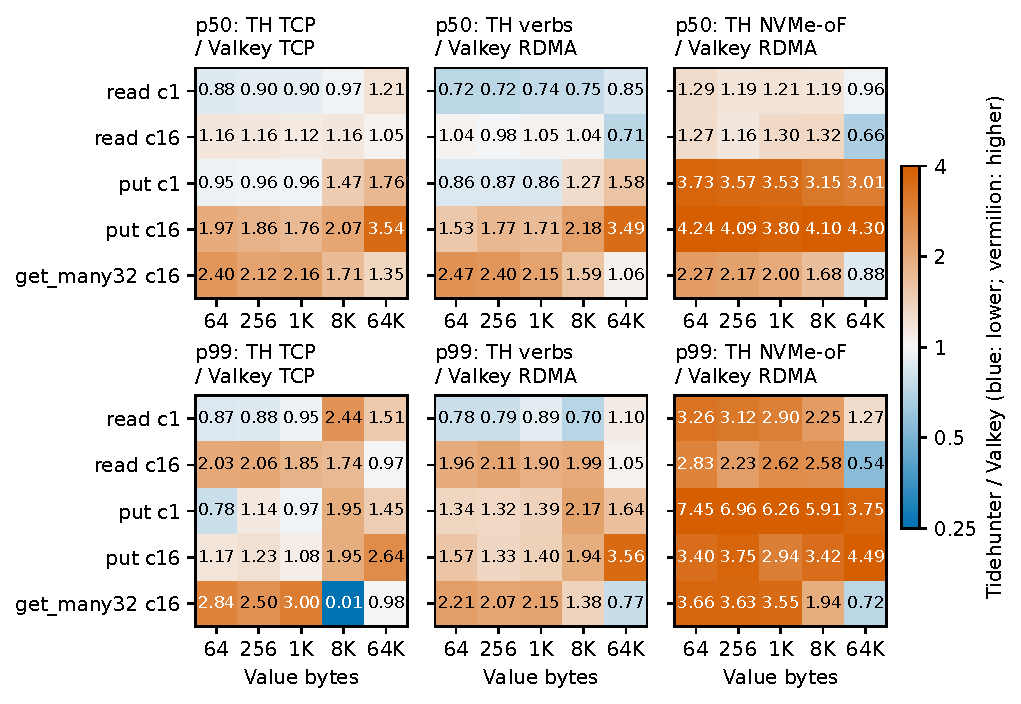
\includegraphics[width=\linewidth]{figures/scoreboard.pdf}
\caption{\carried. \ackB\  Tidehunter/Valkey success-only API p50 (top) and p99 (bottom). Values below one favour Tidehunter. The c1 rows are mixed point operations; other rows are primary c16 cases. \runs. Same CSV inputs and ratios as the 7 November brief.}
\end{figure}
The other stores were not rerun. Each of their cells is the median of per-run quantiles from all GCP runs that completed that population. There are \N{S:ext_pops} such populations and \N{S:ext_runs_min} to \N{S:ext_runs_max} runs per cell. They span fleets, days and sometimes binaries. Their p50 slowest/fastest ratio has median \N{S:ext_spread_med|.2f}, 90th percentile \N{S:ext_spread_p90|.2f}, and maximum \N{S:ext_spread_max|.2f}. This is not a pooled quantile or a matched new-fleet comparison.

\clearpage
\subsection{The unchanged 1 KiB tables}
\begin{table}[H]\centering\fitinput{tab-onekib-1.tex}
\caption{\carried. \ackB\  Scalar calls at c16, success-only API p50 and p99 in \us, successful calls/s. \runs. These tables retain their original keys and CSV inputs.}
\end{table}
\begin{table}[H]\centering\fitinput{tab-onekib-2.tex}
\caption{\carried. \ackB\  32-key calls at c16; API p50/p99 in \us\ and successful calls/s. One call covers 32 values. \runs. Valkey has no batch-write case; a dash is not zero.}
\end{table}
Matched cases have the same cohort, workload, value size, concurrency, operation, key count and offered rate. Concurrency-1 reads use mixed point operations. c16 reads and writes use separate read-only and write-only populations. Do not infer concurrency scaling by treating them as the same mixed workload.

The full-matrix native, Tidehunter and Valkey acknowledgement settings are observed. Garnet uses AOF commit wait; Kvrocks uses RocksDB WAL with sync enabled. Device fsync was not verified for Cassandra, FoundationDB or TiKV. Their write cells are retained but are not durable-contract equivalence claims. Closed-loop successful calls/s is not a production capacity limit.

\clearpage
\subsection{Other stores, unchanged}
\begin{figure}[H]\centering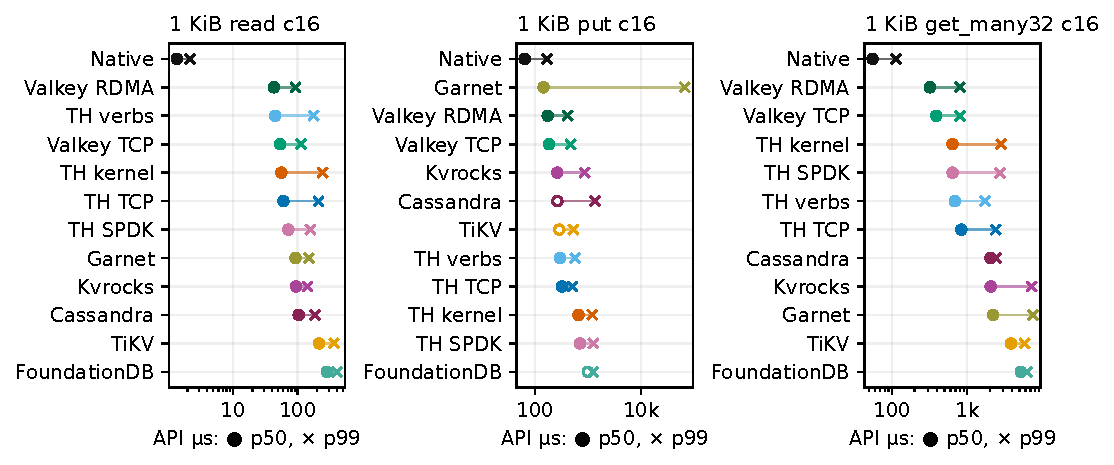
\includegraphics[width=\linewidth]{figures/others.pdf}
\caption{\carried. \ackB\  \ackUnknown\ All stores, 1 KiB c16, sorted by p50. Dots: API p50; crosses: p99. A hollow put dot means device fsync unverified (Cassandra, FoundationDB, TiKV). \runs.}
\end{figure}
\begin{table}[H]\centering\fitinput{tab-stores.tex}
\caption{\carried. \ackB\  \ackUnknown\ API p50/p99 in \us. c1 cells are mixed point operations. \runs. Contracts differ as described above.}
\end{table}
These unchanged data give cross-store context for the retained populations, not a matched-fleet ranking. They do not establish the effect of any later software change. The new stage evidence replaces the old bottleneck interpretation, not these cells.

\clearpage
\subsection{RDMA against TCP and the cache estimate, unchanged}
\begin{figure}[H]\centering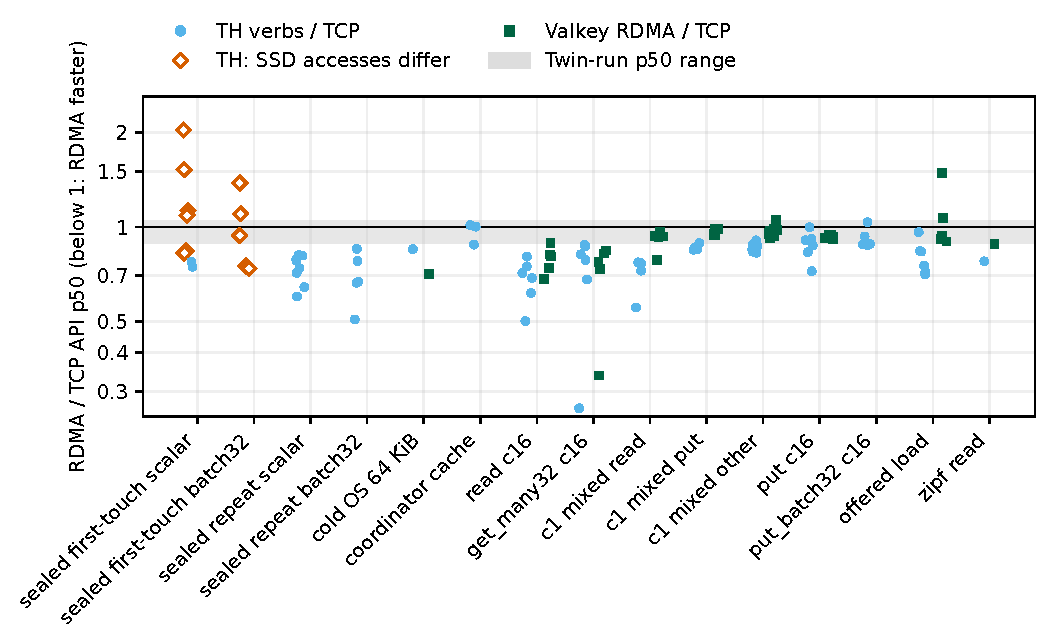
\includegraphics[width=\linewidth]{figures/coherence.pdf}
\caption{\carried. \ackB\  RDMA/TCP API p50 ratios for \N{S:th_pairs} Tidehunter and \N{S:vk_pairs} Valkey workload-matched pairs. Open diamonds mark Tidehunter pairs whose device reads/call differ by more than 0.1. Grey: separate Class A durability-twin p50 context, not a Class B ranking range on the full-matrix fleet. \runs. Tidehunter pairs share that fleet; Valkey ratios divide separate historical medians. Pair-level same-fleet provenance is not established for Valkey.}
\end{figure}
With device-read differences excluded, verbs has the lower p50 in \N{S:th_matched_p50_faster} of \N{S:th_matched} Tidehunter pairs. The other \N{S:th_matched_p50_slower} are near ties. This is a descriptive count, not a universal RDMA advantage. TLS differs between the Tidehunter arms.

\begin{table}[H]\centering\fitinput{tab-hitratio.tex}
\caption{\carried. \ackB\  Estimated cache hit ratio for target mean $g$. Miss cost $L$ is the measured p50; hit cost $H=0.8$~\us\ is the original measured-hit approximation. The estimate $h=(L-g)/(L-H)$ uses medians as proxies for means, so miss tails make it optimistic. It is not a measured hit-ratio curve. \runs.}
\end{table}
This table stays unchanged for continuity. Its cold and miss inputs remain the original full-matrix controls; it is not a new SSD-read decomposition. A coordinator hit avoids the remote path. The achieved hit ratio depends on the workload and memory budget. No Sui KV hit-ratio claim follows from this synthetic campaign.

\clearpage
\section{Next work: ranked decisions}\label{sec:next}
The ranks retain run-8 hypotheses, revisited with the run-9 matched caller grid. Hardware parity is a gate, not a software optimization. Each predicted effect is \inference, not a measured saving. Maintain acknowledgement and validation checks in every A/B run.
Parity also requires equal SSD count and explicit acknowledgement semantics. The five-owner runs remain unmatched to one-SSD Native. Run 9 instead supplies the one-owner matched caller grid, grouped Native controls and same-fleet floors in Section~\ref{sec:rwc}; it does not establish five-owner scale-out. Use its qualification and floor receipts before choosing the next A/B experiment; do not subtract independently sampled floors.

\small\setlength{\tabcolsep}{3pt}
\begin{tabular}{L{.05\linewidth}L{.14\linewidth}L{.24\linewidth}L{.16\linewidth}L{.18\linewidth}L{.10\linewidth}}\toprule
Rank & Item & Measured basis & Expected effect & How to verify & Decision\\\midrule
0 & Hardware parity & Run 8 64 KiB c1 sync means: TCP \N{Y:t:65536:1:mean_us}, verbs \N{Y:v:65536:1:mean_us}, native file+directory \N{Y:n:65536:1:mean_us}~\us. Native cold \N{D:ssd64n:device_reads_per_call|.2f} device ops/call. & \inference\ Separate VM, SSD and allocation hypotheses from owner software, not an additive residual. & Run-9 G13W and both-host read floors are collected (Appendix~\ref{app:rwc-floors}). Match size, host and sync call. Keep Native's mapped/positional read paths unchanged. & Controls collected; no Native rewrite.\\[8pt]
1 & Completion wake-up and network at c1 & Run 8 verbs memory read network \N{C:mem1v:network}~\us; durable put network \N{C:p1v:network}~\us. Run-9 cold/warm calls and successful network controls are separate populations. & \inference\ Reduce completion/stack delay, at a possible CPU cost; not API minus independent floors. & Run-10 trusted TCP/verbs Adaptive/Busy controls; inspect CPU, tails and CQ evidence. Busy also changes client progress, not kernel busy poll. Failed event-write floors stay unavailable. & Run-10 matched ratios/CPU guide policy; no isolated wake-up timer.\\[8pt]
2 & Owner persist and flusher hand-offs at c1 & Run 8 verbs flusher queue mean \N{A:v1:flusher_queue_ns:mean_us}~\us; append-persist exceeds its own fdatasync by \N{A:v1:persist_software_ns:mean_us}~\us. Separate profile: locks+publication \N{P:locks_publication_sum_ns:mean_us|.2f}~\us. Coordinator waits \N{C:p1v:durable}/\N{C:p1v:coalescing}/\N{C:p1v:queue}~\us. & \inference\ Reduce flusher/frontier hand-off and wake-up, not locks. Keep durability. & Time append-persist and storage persist in the same population. Trace flusher and frontier wakes. Do not add nested queue counters. & No durability change.\\[8pt]
3 & Software that grows with value size & Run 8 verbs append-WAL mean \N{A:v1:append_wal_ns:mean_us} to \N{A:v64:append_wal_ns:mean_us}~\us. Unassigned owner mean at 64 KiB: \N{A:v64:handler_remainder_ns:mean_us|.2f}~\us. Coordinator \N{C:p1v:coordinator} to \N{C:p64v:coordinator}~\us. & \inference\ Decode and BLAKE2b verification are candidates, not isolated measured costs. & Run 9 adds one 64 KiB c16 verbs profile; c1 TCP/verbs profile copies remain needed. Time decode, group build and record digest separately. & Ask before digest change: wire and persisted format.\\\bottomrule
\end{tabular}
\normalsize

\clearpage
\subsection{Remaining ranks and evidence gaps}
\small\setlength{\tabcolsep}{3pt}
\begin{tabular}{L{.05\linewidth}L{.14\linewidth}L{.24\linewidth}L{.16\linewidth}L{.18\linewidth}L{.10\linewidth}}\toprule
Rank & Item & Measured basis & Expected effect & How to verify & Decision\\\midrule
4 & Coordinator pipeline waits at c16 & Run 8 verbs timeline: queue \N{C:p16v:queue}, coalescing \N{C:p16v:coalescing}, durable wait \N{C:p16v:durable} of \N{D:p16v:mean_us}~\us\ TOTAL (\N{W:p16v|.1f} percent together). & \inference\ Reduce time between ready work and the next stage. & Trace waits with a tracing-off control at c1 and c16. Report shares of the same-case timeline, not a mixed profile. & Keep bounded queues and group commit.\\[8pt]
5 & Put stall & Run 8 overwrite/new timeline slope \N{Q:run8-stall-fits:0:slope_us_per_put|.3f}/\N{Q:run8-stall-fits:1:slope_us_per_put|.3f}~\us/put; mean spacing \N{Q:run8-stall-fits:0:spacing|.0f}/\N{Q:run8-stall-fits:1:spacing|.0f} puts; median spacing \N{Q:run8-stall-fits:0:median_spacing|.0f}/\N{Q:run8-stall-fits:1:median_spacing|.0f} puts. Run 7 sustained rates fall late. & \inference\ Bound checkpoint work that grows with cumulative puts. & Correlate checkpoint events, stall intervals and cumulative puts; repeat overwrite and new keys. & Identify phase before changing it.\\[8pt]
6 & Batch writes & Run 8 c1, 32$\times$1 KiB p50: native barrier \N{D:batch1n:p50_us}, verbs sync \N{D:batch1v:p50_us}~\us. At 32$\times$8 KiB: \N{D:batch8n:p50_us}/\N{D:ubatch8v:p50_us}~\us. & \inference\ Amortize software without changing the batch contract. & Compare same-shape native and verbs controls. Use batch owner-software and coordinator timers; add repeated controls. & Native batch profiler needed for attribution.\\[8pt]
7 & Hybrid client residual on reads & Run 8 kernel-buffered memory 1 KiB residual \N{C:mem1k:residual}~\us; kernel-direct cold residual \N{C:ssd1k:residual}~\us. & \inference\ Remove client work outside the reader leaves if linked tracing identifies it. & Add dispatch and completion timestamps to the same calls; verify the residual shrinks without moving cost outside the clock. & Run-10 cold controls do not supply linked residual timers.\\\bottomrule
\end{tabular}
\normalsize

\textbf{Run-8 prioritization.} SSD read device time is at the floor (run 8 verbs 1 KiB: \N{C:ssd1v:device}~\us). Verbs TLS is small in its unprofiled put controls: p50 \N{D:uput1m:p50_us}~\us\ versus \N{D:uput1v:p50_us}~\us\ for trusted verbs at 1 KiB c1 (two repetitions). This is descriptive, not significance or an isolated encryption timer. Run 9 does not add the linked timelines, long stall controls, batches or NVMe-oF reads needed to close ranks 4--7.

\textbf{Evidence gaps.} Runs 7/8 lack Native read/batch-write profiles and focused batch reads. Their unprofiled TCP/hybrid batches and hybrid/mTLS deletes are absent; profiles run once. Run 9 completes G13W and the three separate 64 KiB diagnostics (Native c1/c16, owner verbs c16), not c1 TCP/verbs decode/group-build attribution. The old 64 KiB sync gap, stall phase, hybrid residual and excess device reads remain unattributed. No saturation or measured CPU cost supports production capacity.

\clearpage
\section{Provenance and limits}\label{sec:provenance}
\begingroup\small
\RWCtenProvenance

Run 9 uses parent \texttt{bench-bb40628be5664257}, fleet \texttt{bench-41ecdf3f69fb47ec}. Exact launched-package hashes, dirty revision, VM names, UTC times, cleanup and estimated costs are in Appendix~\ref{app:rwc-floors}. The aborted first attempt contributes no results. No historical population is replaced; \path{rwc/generated/inputs-rwc.json} registers the real CSVs, number selectors and per-marker evidence, independently checked by \path{rwc/verify_rwc.py}.

\textbf{Reproduction.} \path{build_run8_inputs.py} copies small CSV tables and derives the flat stall and sustained-rate extracts. It never reads the large decomposition export or summary JSON. \path{inputs.json} stores source and output SHA-256 hashes. \path{data.py} extends the original number language. \path{make_tables.py} resolves all \texttt{\textbackslash N\{key\}} values and stops on an unknown or ambiguous selection. \path{plot_final.py} makes vector PDFs. \path{evidence.json} records each point's case id, source values, run, fleet, contract and repetitions. The appendix lists every operation population of run 8, including diagnostic copies.

The full-matrix section copies the seven versioned CSV inputs from the 7 November brief. It preserves the scoreboard, two 1 KiB tables, other-stores figure/table, transport coherence and hit-ratio table. It does not regenerate that brief's inputs: its extraction script needs the unavailable 12 GB export. Its old remote-NVMe interpretation and bottleneck ranking are replaced here.

\textbf{Source corrections.} The native 1 KiB memory time in the run-8 narrative is explicitly from run 6, not a run-8 case; it is not imported here. The native column in that narrative's write-components table places file sync under owner persist; the component CSV places it under durable wait. We follow the CSV and state the native label. Its directory sync remains in the residual, not in a fabricated leaf.

\path{run8-cold_resident.csv} retains the original analysis table, but is not used to compare concurrency. Its two owner c16 cold rows select a c1 resident partner, and its mTLS route label differs from \path{ops_summary.csv}. Our explicit selection uses group, route, concurrency, state, contract and instrument and rejects ambiguity. \path{failed_cases.csv} retains outer size metadata of 64 KiB for the direct-write failures, while the write-floor table identifies the actual failed 1 KiB block. We use the block size, not that outer metadata.

The run-7 report and \path{APPLES-TO-APPLES.md} subtract run-6 memory timings from run-7 SSD timings. We do not carry that cross-fleet subtraction forward. Their observations do not create a measured component. The earlier brief's late-rate estimate included a partial final bucket and was biased low. The corrected \path{analysis-final-v2/output/} uses the last five complete one-second buckets and agrees in range with the report headline. The focused campaign's historical ``Deferred'' paragraph predates the successful direct-kernel fleet runs; later launch history supersedes it.

\textbf{Limits.} Runs 7 and 8 each have one client and five owners of the same VM class and region; equal class is not hardware parity. The run-7 random dataset has 65,536 keys. It does not cover authority-history misses. Small SSD-read populations are bimodal. Their p50 can change while their means remain similar. Profiles perturb calls, and some exported leaves are derived means with only count equality, not a proved per-call join. Their additive arithmetic is bookkeeping, not an exact physical partition. Native whole-call means in the read figure aggregate two per-repetition means; they are not one profiled call population. Full case metadata stays in the copied tables.

No claim establishes physical NAND service per call, isolated wire time, significance, serializable transactions, permanent-loss tolerance, failover or production capacity. The authorized run-9 campaign supplied new measurements; document generation launches nothing. Native remains unchanged. Its six unqualified cold cases and the three failed event-write floor controls are retained, not hidden or zeroed. Preserve durability and security contracts.

\endgroup

\appendix
\clearpage\section{Durable scalar puts}
Run 8, focused unified fleet. Each row is one CSV population, not pooled calls. API statistics are in \us. With two repetitions each cell is the median of per-repetition statistics. $n$ lists successful calls in each repetition; $r$ counts repetitions. B: native barrier; P: native page cache; S: owner synchronous; N: owner page cache. T: timeline; W: write profile; R: read profile; --: no profile. Row ids map to the zero-based row of \path{run8-ops_summary.csv}.
\begin{center}\scriptsize\setlength{\tabcolsep}{3pt}
\begin{tabular}{llrrrrrrrrr}\toprule
Id/diag & Route/contract & KiB & $c$ & $n$ & $r$ & mean & p50 & p99 & p99.9 & State\\\midrule
031/T & verbs/S & 1 & 1 & \N{D:op031:n} & 1 & \N{D:op031:mean_us} & \N{D:op031:p50_us} & \N{D:op031:p99_us} & \N{D:op031:p999_us} & put\\
032/W & verbs/S & 1 & 1 & \N{D:op032:n} & 1 & \N{D:op032:mean_us} & \N{D:op032:p50_us} & \N{D:op032:p99_us} & \N{D:op032:p999_us} & put\\
036/W & native/B & 64 & 1 & \N{D:op036:n} & 1 & \N{D:op036:mean_us} & \N{D:op036:p50_us} & \N{D:op036:p99_us} & \N{D:op036:p999_us} & put\\
037/T & TCP/S & 1 & 16 & \N{D:op037:n} & 1 & \N{D:op037:mean_us} & \N{D:op037:p50_us} & \N{D:op037:p99_us} & \N{D:op037:p999_us} & put\\
038/W & verbs/S & 1 & 16 & \N{D:op038:n} & 1 & \N{D:op038:mean_us} & \N{D:op038:p50_us} & \N{D:op038:p99_us} & \N{D:op038:p999_us} & put\\
039/T & mTLS/S & 1 & 1 & \N{D:op039:n} & 1 & \N{D:op039:mean_us} & \N{D:op039:p50_us} & \N{D:op039:p99_us} & \N{D:op039:p999_us} & put\\
042/T & verbs/S & 1 & 16 & \N{D:op042:n} & 1 & \N{D:op042:mean_us} & \N{D:op042:p50_us} & \N{D:op042:p99_us} & \N{D:op042:p999_us} & put\\
044/T & TCP/S & 1 & 1 & \N{D:op044:n} & 1 & \N{D:op044:mean_us} & \N{D:op044:p50_us} & \N{D:op044:p99_us} & \N{D:op044:p999_us} & put\\
045/T & verbs/S & 64 & 1 & \N{D:op045:n} & 1 & \N{D:op045:mean_us} & \N{D:op045:p50_us} & \N{D:op045:p99_us} & \N{D:op045:p999_us} & put\\
046/W & native/B & 1 & 1 & \N{D:op046:n} & 1 & \N{D:op046:mean_us} & \N{D:op046:p50_us} & \N{D:op046:p99_us} & \N{D:op046:p999_us} & put\\
047/T & kernel D/S & 1 & 1 & \N{D:op047:n} & 1 & \N{D:op047:mean_us} & \N{D:op047:p50_us} & \N{D:op047:p99_us} & \N{D:op047:p999_us} & put\\
049/W & native/B & 1 & 16 & \N{D:op049:n} & 1 & \N{D:op049:mean_us} & \N{D:op049:p50_us} & \N{D:op049:p99_us} & \N{D:op049:p999_us} & put\\
050/T & TCP/S & 64 & 1 & \N{D:op050:n} & 1 & \N{D:op050:mean_us} & \N{D:op050:p50_us} & \N{D:op050:p99_us} & \N{D:op050:p999_us} & put\\
051/T & SPDK/S & 1 & 1 & \N{D:op051:n} & 1 & \N{D:op051:mean_us} & \N{D:op051:p50_us} & \N{D:op051:p99_us} & \N{D:op051:p999_us} & put\\
052/-- & SPDK/S & 64 & 16 & \N{D:op052:n} & 2 & \N{D:op052:mean_us} & \N{D:op052:p50_us} & \N{D:op052:p99_us} & \N{D:op052:p999_us} & put\\
053/-- & kernel D/S & 64 & 16 & \N{D:op053:n} & 2 & \N{D:op053:mean_us} & \N{D:op053:p50_us} & \N{D:op053:p99_us} & \N{D:op053:p999_us} & put\\
054/-- & SPDK/S & 1 & 1 & \N{D:op054:n} & 2 & \N{D:op054:mean_us} & \N{D:op054:p50_us} & \N{D:op054:p99_us} & \N{D:op054:p999_us} & put\\
055/-- & kernel D/S & 1 & 1 & \N{D:op055:n} & 2 & \N{D:op055:mean_us} & \N{D:op055:p50_us} & \N{D:op055:p99_us} & \N{D:op055:p999_us} & put\\
056/-- & SPDK/S & 1 & 16 & \N{D:op056:n} & 2 & \N{D:op056:mean_us} & \N{D:op056:p50_us} & \N{D:op056:p99_us} & \N{D:op056:p999_us} & put\\
057/-- & kernel D/S & 1 & 16 & \N{D:op057:n} & 2 & \N{D:op057:mean_us} & \N{D:op057:p50_us} & \N{D:op057:p99_us} & \N{D:op057:p999_us} & put\\
058/-- & verbs/S & 1 & 1 & \N{D:op058:n} & 2 & \N{D:op058:mean_us} & \N{D:op058:p50_us} & \N{D:op058:p99_us} & \N{D:op058:p999_us} & put/new\\
059/-- & native/B & 1 & 1 & \N{D:op059:n} & 2 & \N{D:op059:mean_us} & \N{D:op059:p50_us} & \N{D:op059:p99_us} & \N{D:op059:p999_us} & put/new\\
060/-- & verbs/S & 1 & 16 & \N{D:op060:n} & 2 & \N{D:op060:mean_us} & \N{D:op060:p50_us} & \N{D:op060:p99_us} & \N{D:op060:p999_us} & put/new\\
061/-- & native/B & 1 & 16 & \N{D:op061:n} & 2 & \N{D:op061:mean_us} & \N{D:op061:p50_us} & \N{D:op061:p99_us} & \N{D:op061:p999_us} & put/new\\
062/-- & verbs/S & 64 & 16 & \N{D:op062:n} & 2 & \N{D:op062:mean_us} & \N{D:op062:p50_us} & \N{D:op062:p99_us} & \N{D:op062:p999_us} & put/new\\
063/-- & native/B & 64 & 16 & \N{D:op063:n} & 2 & \N{D:op063:mean_us} & \N{D:op063:p50_us} & \N{D:op063:p99_us} & \N{D:op063:p999_us} & put/new\\
064/-- & native/B & 8 & 16 & \N{D:op064:n} & 2 & \N{D:op064:mean_us} & \N{D:op064:p50_us} & \N{D:op064:p99_us} & \N{D:op064:p999_us} & put\\
067/-- & native/B & 8 & 1 & \N{D:op067:n} & 2 & \N{D:op067:mean_us} & \N{D:op067:p50_us} & \N{D:op067:p99_us} & \N{D:op067:p999_us} & put\\
075/-- & native/B & 64 & 16 & \N{D:op075:n} & 2 & \N{D:op075:mean_us} & \N{D:op075:p50_us} & \N{D:op075:p99_us} & \N{D:op075:p999_us} & put\\
081/-- & native/B & 64 & 1 & \N{D:op081:n} & 2 & \N{D:op081:mean_us} & \N{D:op081:p50_us} & \N{D:op081:p99_us} & \N{D:op081:p999_us} & put\\
082/-- & native/B & 1 & 16 & \N{D:op082:n} & 2 & \N{D:op082:mean_us} & \N{D:op082:p50_us} & \N{D:op082:p99_us} & \N{D:op082:p999_us} & put\\
086/-- & native/B & 1 & 1 & \N{D:op086:n} & 2 & \N{D:op086:mean_us} & \N{D:op086:p50_us} & \N{D:op086:p99_us} & \N{D:op086:p999_us} & put\\
\bottomrule\end{tabular}\end{center}
Native barrier uses one process and one SSD against five owners. Its per-put file and directory fsync is not owner covering fdatasync. The c16 64 KiB result therefore is not a local-path latency lower bound.
\clearpage\section{Durable scalar puts (continued)}
Run 8, focused unified fleet. Each row is one CSV population, not pooled calls. API statistics are in \us. With two repetitions each cell is the median of per-repetition statistics. $n$ lists successful calls in each repetition; $r$ counts repetitions. B: native barrier; P: native page cache; S: owner synchronous; N: owner page cache. T: timeline; W: write profile; R: read profile; --: no profile. Row ids map to the zero-based row of \path{run8-ops_summary.csv}.
\begin{center}\scriptsize\setlength{\tabcolsep}{3pt}
\begin{tabular}{llrrrrrrrrr}\toprule
Id/diag & Route/contract & KiB & $c$ & $n$ & $r$ & mean & p50 & p99 & p99.9 & State\\\midrule
088/T & verbs/S & 1 & 16 & \N{D:op088:n} & 1 & \N{D:op088:mean_us} & \N{D:op088:p50_us} & \N{D:op088:p99_us} & \N{D:op088:p999_us} & put\\
089/W & verbs/S & 1 & 16 & \N{D:op089:n} & 1 & \N{D:op089:mean_us} & \N{D:op089:p50_us} & \N{D:op089:p99_us} & \N{D:op089:p999_us} & put\\
090/T & verbs/S & 1 & 16 & \N{D:op090:n} & 1 & \N{D:op090:mean_us} & \N{D:op090:p50_us} & \N{D:op090:p99_us} & \N{D:op090:p999_us} & put/new\\
091/W & verbs/S & 1 & 16 & \N{D:op091:n} & 1 & \N{D:op091:mean_us} & \N{D:op091:p50_us} & \N{D:op091:p99_us} & \N{D:op091:p999_us} & put/new\\
095/-- & verbs/S & 8 & 16 & \N{D:op095:n} & 2 & \N{D:op095:mean_us} & \N{D:op095:p50_us} & \N{D:op095:p99_us} & \N{D:op095:p999_us} & put\\
096/-- & mTLS/S & 1 & 16 & \N{D:op096:n} & 2 & \N{D:op096:mean_us} & \N{D:op096:p50_us} & \N{D:op096:p99_us} & \N{D:op096:p999_us} & put\\
097/-- & verbs/S & 64 & 1 & \N{D:op097:n} & 2 & \N{D:op097:mean_us} & \N{D:op097:p50_us} & \N{D:op097:p99_us} & \N{D:op097:p999_us} & put\\
099/-- & mTLS/S & 64 & 1 & \N{D:op099:n} & 2 & \N{D:op099:mean_us} & \N{D:op099:p50_us} & \N{D:op099:p99_us} & \N{D:op099:p999_us} & put\\
101/-- & TCP/S & 64 & 1 & \N{D:op101:n} & 2 & \N{D:op101:mean_us} & \N{D:op101:p50_us} & \N{D:op101:p99_us} & \N{D:op101:p999_us} & put\\
102/-- & verbs/S & 1 & 16 & \N{D:op102:n} & 2 & \N{D:op102:mean_us} & \N{D:op102:p50_us} & \N{D:op102:p99_us} & \N{D:op102:p999_us} & put\\
106/-- & mTLS/S & 1 & 1 & \N{D:op106:n} & 2 & \N{D:op106:mean_us} & \N{D:op106:p50_us} & \N{D:op106:p99_us} & \N{D:op106:p999_us} & put\\
110/-- & verbs/S & 64 & 16 & \N{D:op110:n} & 2 & \N{D:op110:mean_us} & \N{D:op110:p50_us} & \N{D:op110:p99_us} & \N{D:op110:p999_us} & put\\
111/-- & TCP/S & 1 & 16 & \N{D:op111:n} & 2 & \N{D:op111:mean_us} & \N{D:op111:p50_us} & \N{D:op111:p99_us} & \N{D:op111:p999_us} & put\\
112/-- & mTLS/S & 64 & 16 & \N{D:op112:n} & 2 & \N{D:op112:mean_us} & \N{D:op112:p50_us} & \N{D:op112:p99_us} & \N{D:op112:p999_us} & put\\
116/-- & TCP/S & 1 & 1 & \N{D:op116:n} & 2 & \N{D:op116:mean_us} & \N{D:op116:p50_us} & \N{D:op116:p99_us} & \N{D:op116:p999_us} & put\\
121/-- & verbs/S & 1 & 1 & \N{D:op121:n} & 2 & \N{D:op121:mean_us} & \N{D:op121:p50_us} & \N{D:op121:p99_us} & \N{D:op121:p999_us} & put\\
122/-- & TCP/S & 64 & 16 & \N{D:op122:n} & 2 & \N{D:op122:mean_us} & \N{D:op122:p50_us} & \N{D:op122:p99_us} & \N{D:op122:p999_us} & put\\
125/-- & verbs/S & 8 & 1 & \N{D:op125:n} & 2 & \N{D:op125:mean_us} & \N{D:op125:p50_us} & \N{D:op125:p99_us} & \N{D:op125:p999_us} & put\\
\bottomrule\end{tabular}\end{center}
Native barrier uses one process and one SSD against five owners. Its per-put file and directory fsync is not owner covering fdatasync. The c16 64 KiB result therefore is not a local-path latency lower bound.
\clearpage\section{Page-cache-acknowledged scalar puts}
Run 8, focused unified fleet. Each row is one CSV population, not pooled calls. API statistics are in \us. With two repetitions each cell is the median of per-repetition statistics. $n$ lists successful calls in each repetition; $r$ counts repetitions. B: native barrier; P: native page cache; S: owner synchronous; N: owner page cache. T: timeline; W: write profile; R: read profile; --: no profile. Row ids map to the zero-based row of \path{run8-ops_summary.csv}.
\begin{center}\scriptsize\setlength{\tabcolsep}{3pt}
\begin{tabular}{llrrrrrrrrr}\toprule
Id/diag & Route/contract & KiB & $c$ & $n$ & $r$ & mean & p50 & p99 & p99.9 & State\\\midrule
035/T & verbs/N & 1 & 1 & \N{D:op035:n} & 1 & \N{D:op035:mean_us} & \N{D:op035:p50_us} & \N{D:op035:p99_us} & \N{D:op035:p999_us} & put\\
043/W & native/P & 1 & 1 & \N{D:op043:n} & 1 & \N{D:op043:mean_us} & \N{D:op043:p50_us} & \N{D:op043:p99_us} & \N{D:op043:p999_us} & put\\
069/-- & native/P & 64 & 16 & \N{D:op069:n} & 2 & \N{D:op069:mean_us} & \N{D:op069:p50_us} & \N{D:op069:p99_us} & \N{D:op069:p999_us} & put\\
070/-- & native/P & 1 & 1 & \N{D:op070:n} & 2 & \N{D:op070:mean_us} & \N{D:op070:p50_us} & \N{D:op070:p99_us} & \N{D:op070:p999_us} & put\\
071/-- & native/P & 8 & 16 & \N{D:op071:n} & 2 & \N{D:op071:mean_us} & \N{D:op071:p50_us} & \N{D:op071:p99_us} & \N{D:op071:p999_us} & put\\
076/-- & native/P & 8 & 1 & \N{D:op076:n} & 2 & \N{D:op076:mean_us} & \N{D:op076:p50_us} & \N{D:op076:p99_us} & \N{D:op076:p999_us} & put\\
077/-- & native/P & 1 & 16 & \N{D:op077:n} & 2 & \N{D:op077:mean_us} & \N{D:op077:p50_us} & \N{D:op077:p99_us} & \N{D:op077:p999_us} & put\\
083/-- & native/P & 64 & 1 & \N{D:op083:n} & 2 & \N{D:op083:mean_us} & \N{D:op083:p50_us} & \N{D:op083:p99_us} & \N{D:op083:p999_us} & put\\
092/-- & TCP/N & 64 & 1 & \N{D:op092:n} & 2 & \N{D:op092:mean_us} & \N{D:op092:p50_us} & \N{D:op092:p99_us} & \N{D:op092:p999_us} & put\\
098/-- & TCP/N & 1 & 1 & \N{D:op098:n} & 2 & \N{D:op098:mean_us} & \N{D:op098:p50_us} & \N{D:op098:p99_us} & \N{D:op098:p999_us} & put\\
100/-- & TCP/N & 64 & 16 & \N{D:op100:n} & 2 & \N{D:op100:mean_us} & \N{D:op100:p50_us} & \N{D:op100:p99_us} & \N{D:op100:p999_us} & put\\
104/-- & verbs/N & 64 & 1 & \N{D:op104:n} & 2 & \N{D:op104:mean_us} & \N{D:op104:p50_us} & \N{D:op104:p99_us} & \N{D:op104:p999_us} & put\\
105/-- & verbs/N & 8 & 1 & \N{D:op105:n} & 2 & \N{D:op105:mean_us} & \N{D:op105:p50_us} & \N{D:op105:p99_us} & \N{D:op105:p999_us} & put\\
107/-- & verbs/N & 64 & 16 & \N{D:op107:n} & 2 & \N{D:op107:mean_us} & \N{D:op107:p50_us} & \N{D:op107:p99_us} & \N{D:op107:p999_us} & put\\
119/-- & verbs/N & 1 & 16 & \N{D:op119:n} & 2 & \N{D:op119:mean_us} & \N{D:op119:p50_us} & \N{D:op119:p99_us} & \N{D:op119:p999_us} & put\\
120/-- & verbs/N & 1 & 1 & \N{D:op120:n} & 2 & \N{D:op120:mean_us} & \N{D:op120:p50_us} & \N{D:op120:p99_us} & \N{D:op120:p999_us} & put\\
124/-- & TCP/N & 1 & 16 & \N{D:op124:n} & 2 & \N{D:op124:mean_us} & \N{D:op124:p50_us} & \N{D:op124:p99_us} & \N{D:op124:p999_us} & put\\
126/-- & verbs/N & 8 & 16 & \N{D:op126:n} & 2 & \N{D:op126:mean_us} & \N{D:op126:p50_us} & \N{D:op126:p99_us} & \N{D:op126:p999_us} & put\\
\bottomrule\end{tabular}\end{center}
\clearpage\section{Batch writes and deletes}
Run 8, focused unified fleet. Each row is one CSV population, not pooled calls. API statistics are in \us. With two repetitions each cell is the median of per-repetition statistics. $n$ lists successful calls in each repetition; $r$ counts repetitions. B: native barrier; P: native page cache; S: owner synchronous; N: owner page cache. T: timeline; W: write profile; R: read profile; --: no profile. Row ids map to the zero-based row of \path{run8-ops_summary.csv}.
\begin{center}\scriptsize\setlength{\tabcolsep}{3pt}
\begin{tabular}{llrrrrrrrrr}\toprule
Id/diag & Route/contract & KiB & $c$ & $n$ & $r$ & mean & p50 & p99 & p99.9 & State\\\midrule
033/T & verbs/S & 8 & 1 & \N{D:op033:n} & 1 & \N{D:op033:mean_us} & \N{D:op033:p50_us} & \N{D:op033:p99_us} & \N{D:op033:p999_us} & batch\\
034/T & verbs/S & 1 & 1 & \N{D:op034:n} & 1 & \N{D:op034:mean_us} & \N{D:op034:p50_us} & \N{D:op034:p99_us} & \N{D:op034:p999_us} & delete\\
040/T & TCP/S & 1 & 1 & \N{D:op040:n} & 1 & \N{D:op040:mean_us} & \N{D:op040:p50_us} & \N{D:op040:p99_us} & \N{D:op040:p999_us} & delete\\
041/W & native/B & 1 & 1 & \N{D:op041:n} & 1 & \N{D:op041:mean_us} & \N{D:op041:p50_us} & \N{D:op041:p99_us} & \N{D:op041:p999_us} & delete\\
048/T & TCP/S & 8 & 1 & \N{D:op048:n} & 1 & \N{D:op048:mean_us} & \N{D:op048:p50_us} & \N{D:op048:p99_us} & \N{D:op048:p999_us} & batch\\
065/-- & native/P & 8 & 1 & \N{D:op065:n} & 1 & \N{D:op065:mean_us} & \N{D:op065:p50_us} & \N{D:op065:p99_us} & \N{D:op065:p999_us} & batch\\
066/-- & native/B & 1 & 1 & \N{D:op066:n} & 1 & \N{D:op066:mean_us} & \N{D:op066:p50_us} & \N{D:op066:p99_us} & \N{D:op066:p999_us} & batch\\
068/-- & native/P & 1 & 1 & \N{D:op068:n} & 1 & \N{D:op068:mean_us} & \N{D:op068:p50_us} & \N{D:op068:p99_us} & \N{D:op068:p999_us} & batch\\
072/-- & native/P & 8 & 16 & \N{D:op072:n} & 1 & \N{D:op072:mean_us} & \N{D:op072:p50_us} & \N{D:op072:p99_us} & \N{D:op072:p999_us} & batch\\
073/-- & native/P & 1 & 1 & \N{D:op073:n} & 1 & \N{D:op073:mean_us} & \N{D:op073:p50_us} & \N{D:op073:p99_us} & \N{D:op073:p999_us} & delete\\
074/-- & native/B & 1 & 16 & \N{D:op074:n} & 1 & \N{D:op074:mean_us} & \N{D:op074:p50_us} & \N{D:op074:p99_us} & \N{D:op074:p999_us} & batch\\
078/-- & native/B & 1 & 16 & \N{D:op078:n} & 1 & \N{D:op078:mean_us} & \N{D:op078:p50_us} & \N{D:op078:p99_us} & \N{D:op078:p999_us} & delete\\
079/-- & native/B & 8 & 1 & \N{D:op079:n} & 1 & \N{D:op079:mean_us} & \N{D:op079:p50_us} & \N{D:op079:p99_us} & \N{D:op079:p999_us} & batch\\
080/-- & native/P & 1 & 16 & \N{D:op080:n} & 1 & \N{D:op080:mean_us} & \N{D:op080:p50_us} & \N{D:op080:p99_us} & \N{D:op080:p999_us} & delete\\
084/-- & native/P & 1 & 16 & \N{D:op084:n} & 1 & \N{D:op084:mean_us} & \N{D:op084:p50_us} & \N{D:op084:p99_us} & \N{D:op084:p999_us} & batch\\
085/-- & native/B & 8 & 16 & \N{D:op085:n} & 1 & \N{D:op085:mean_us} & \N{D:op085:p50_us} & \N{D:op085:p99_us} & \N{D:op085:p999_us} & batch\\
087/-- & native/B & 1 & 1 & \N{D:op087:n} & 1 & \N{D:op087:mean_us} & \N{D:op087:p50_us} & \N{D:op087:p99_us} & \N{D:op087:p999_us} & delete\\
093/-- & verbs/S & 8 & 16 & \N{D:op093:n} & 1 & \N{D:op093:mean_us} & \N{D:op093:p50_us} & \N{D:op093:p99_us} & \N{D:op093:p999_us} & batch\\
094/-- & verbs/N & 1 & 1 & \N{D:op094:n} & 1 & \N{D:op094:mean_us} & \N{D:op094:p50_us} & \N{D:op094:p99_us} & \N{D:op094:p999_us} & batch\\
103/-- & verbs/S & 1 & 16 & \N{D:op103:n} & 1 & \N{D:op103:mean_us} & \N{D:op103:p50_us} & \N{D:op103:p99_us} & \N{D:op103:p999_us} & delete\\
108/-- & verbs/N & 1 & 16 & \N{D:op108:n} & 1 & \N{D:op108:mean_us} & \N{D:op108:p50_us} & \N{D:op108:p99_us} & \N{D:op108:p999_us} & delete\\
109/-- & verbs/N & 8 & 1 & \N{D:op109:n} & 1 & \N{D:op109:mean_us} & \N{D:op109:p50_us} & \N{D:op109:p99_us} & \N{D:op109:p999_us} & batch\\
113/-- & verbs/N & 1 & 1 & \N{D:op113:n} & 1 & \N{D:op113:mean_us} & \N{D:op113:p50_us} & \N{D:op113:p99_us} & \N{D:op113:p999_us} & delete\\
114/-- & verbs/S & 1 & 1 & \N{D:op114:n} & 1 & \N{D:op114:mean_us} & \N{D:op114:p50_us} & \N{D:op114:p99_us} & \N{D:op114:p999_us} & batch\\
115/-- & verbs/S & 8 & 1 & \N{D:op115:n} & 1 & \N{D:op115:mean_us} & \N{D:op115:p50_us} & \N{D:op115:p99_us} & \N{D:op115:p999_us} & batch\\
117/-- & verbs/N & 1 & 16 & \N{D:op117:n} & 1 & \N{D:op117:mean_us} & \N{D:op117:p50_us} & \N{D:op117:p99_us} & \N{D:op117:p999_us} & batch\\
118/-- & verbs/S & 1 & 1 & \N{D:op118:n} & 1 & \N{D:op118:mean_us} & \N{D:op118:p50_us} & \N{D:op118:p99_us} & \N{D:op118:p999_us} & delete\\
123/-- & verbs/S & 1 & 16 & \N{D:op123:n} & 1 & \N{D:op123:mean_us} & \N{D:op123:p50_us} & \N{D:op123:p99_us} & \N{D:op123:p999_us} & batch\\
127/-- & verbs/N & 8 & 16 & \N{D:op127:n} & 1 & \N{D:op127:mean_us} & \N{D:op127:p50_us} & \N{D:op127:p99_us} & \N{D:op127:p999_us} & batch\\
\bottomrule\end{tabular}\end{center}
\clearpage\section{Reads}
Run 8, focused unified fleet. Each row is one CSV population, not pooled calls. API statistics are in \us. With two repetitions each cell is the median of per-repetition statistics. $n$ lists successful calls in each repetition; $r$ counts repetitions. B: native barrier; P: native page cache; S: owner synchronous; N: owner page cache. T: timeline; W: write profile; R: read profile; --: no profile. Row ids map to the zero-based row of \path{run8-ops_summary.csv}.
\begin{center}\scriptsize\setlength{\tabcolsep}{3pt}
\begin{tabular}{llrrrrrrrrr}\toprule
Id/diag & Route/contract & KiB & $c$ & $n$ & $r$ & mean & p50 & p99 & p99.9 & State\\\midrule
000/R & TCP/S & 64 & 1 & \N{D:op000:n} & 1 & \N{D:op000:mean_us} & \N{D:op000:p50_us} & \N{D:op000:p99_us} & \N{D:op000:p999_us} & cold\\
001/R & verbs/S & 1 & 1 & \N{D:op001:n} & 1 & \N{D:op001:mean_us} & \N{D:op001:p50_us} & \N{D:op001:p99_us} & \N{D:op001:p999_us} & cold\\
002/R & TCP/S & 1 & 16 & \N{D:op002:n} & 1 & \N{D:op002:mean_us} & \N{D:op002:p50_us} & \N{D:op002:p99_us} & \N{D:op002:p999_us} & cold\\
003/R & SPDK/S & 64 & 1 & \N{D:op003:n} & 1 & \N{D:op003:mean_us} & \N{D:op003:p50_us} & \N{D:op003:p99_us} & \N{D:op003:p999_us} & cold\\
004/R & kernel D/S & 1 & 1 & \N{D:op004:n} & 1 & \N{D:op004:mean_us} & \N{D:op004:p50_us} & \N{D:op004:p99_us} & \N{D:op004:p999_us} & cold\\
005/R & verbs/S & 1 & 16 & \N{D:op005:n} & 1 & \N{D:op005:mean_us} & \N{D:op005:p50_us} & \N{D:op005:p99_us} & \N{D:op005:p999_us} & cold\\
006/R & SPDK/S & 1 & 16 & \N{D:op006:n} & 1 & \N{D:op006:mean_us} & \N{D:op006:p50_us} & \N{D:op006:p99_us} & \N{D:op006:p999_us} & cold\\
007/R & mTLS/S & 1 & 1 & \N{D:op007:n} & 1 & \N{D:op007:mean_us} & \N{D:op007:p50_us} & \N{D:op007:p99_us} & \N{D:op007:p999_us} & cold\\
008/R & kernel D/S & 1 & 16 & \N{D:op008:n} & 1 & \N{D:op008:mean_us} & \N{D:op008:p50_us} & \N{D:op008:p99_us} & \N{D:op008:p999_us} & cold\\
009/R & TCP/S & 1 & 1 & \N{D:op009:n} & 1 & \N{D:op009:mean_us} & \N{D:op009:p50_us} & \N{D:op009:p99_us} & \N{D:op009:p999_us} & cold\\
010/R & verbs/S & 64 & 1 & \N{D:op010:n} & 1 & \N{D:op010:mean_us} & \N{D:op010:p50_us} & \N{D:op010:p99_us} & \N{D:op010:p999_us} & cold\\
011/R & SPDK/S & 1 & 1 & \N{D:op011:n} & 1 & \N{D:op011:mean_us} & \N{D:op011:p50_us} & \N{D:op011:p99_us} & \N{D:op011:p999_us} & cold\\
012/R & kernel D/S & 64 & 1 & \N{D:op012:n} & 1 & \N{D:op012:mean_us} & \N{D:op012:p50_us} & \N{D:op012:p99_us} & \N{D:op012:p999_us} & cold\\
013/-- & native/B & 1 & 16 & \N{D:op013:n} & 1 & \N{D:op013:mean_us} & \N{D:op013:p50_us} & \N{D:op013:p99_us} & \N{D:op013:p999_us} & cold\\
014/-- & native/B & 64 & 16 & \N{D:op014:n} & 1 & \N{D:op014:mean_us} & \N{D:op014:p50_us} & \N{D:op014:p99_us} & \N{D:op014:p999_us} & cold\\
015/-- & native/B & 1 & 1 & \N{D:op015:n} & 2 & \N{D:op015:mean_us} & \N{D:op015:p50_us} & \N{D:op015:p99_us} & \N{D:op015:p999_us} & cold\\
016/-- & native/B & 8 & 1 & \N{D:op016:n} & 2 & \N{D:op016:mean_us} & \N{D:op016:p50_us} & \N{D:op016:p99_us} & \N{D:op016:p999_us} & cold\\
017/-- & native/B & 64 & 1 & \N{D:op017:n} & 2 & \N{D:op017:mean_us} & \N{D:op017:p50_us} & \N{D:op017:p99_us} & \N{D:op017:p999_us} & cold\\
018/R & kernel B/S & 1 & 1 & \N{D:op018:n} & 1 & \N{D:op018:mean_us} & \N{D:op018:p50_us} & \N{D:op018:p99_us} & \N{D:op018:p999_us} & memory\\
019/R & TCP/S & 64 & 1 & \N{D:op019:n} & 1 & \N{D:op019:mean_us} & \N{D:op019:p50_us} & \N{D:op019:p99_us} & \N{D:op019:p999_us} & memory\\
020/R & verbs/S & 1 & 1 & \N{D:op020:n} & 1 & \N{D:op020:mean_us} & \N{D:op020:p50_us} & \N{D:op020:p99_us} & \N{D:op020:p999_us} & memory\\
021/R & TCP/S & 1 & 16 & \N{D:op021:n} & 1 & \N{D:op021:mean_us} & \N{D:op021:p50_us} & \N{D:op021:p99_us} & \N{D:op021:p999_us} & memory\\
022/R & kernel B/S & 64 & 1 & \N{D:op022:n} & 1 & \N{D:op022:mean_us} & \N{D:op022:p50_us} & \N{D:op022:p99_us} & \N{D:op022:p999_us} & memory\\
023/R & mTLS/S & 1 & 1 & \N{D:op023:n} & 1 & \N{D:op023:mean_us} & \N{D:op023:p50_us} & \N{D:op023:p99_us} & \N{D:op023:p999_us} & memory\\
024/R & verbs/S & 1 & 16 & \N{D:op024:n} & 1 & \N{D:op024:mean_us} & \N{D:op024:p50_us} & \N{D:op024:p99_us} & \N{D:op024:p999_us} & memory\\
025/R & verbs/S & 64 & 1 & \N{D:op025:n} & 1 & \N{D:op025:mean_us} & \N{D:op025:p50_us} & \N{D:op025:p99_us} & \N{D:op025:p999_us} & memory\\
026/R & TCP/S & 1 & 1 & \N{D:op026:n} & 1 & \N{D:op026:mean_us} & \N{D:op026:p50_us} & \N{D:op026:p99_us} & \N{D:op026:p999_us} & memory\\
027/-- & native/B & 64 & 1 & \N{D:op027:n} & 2 & \N{D:op027:mean_us} & \N{D:op027:p50_us} & \N{D:op027:p99_us} & \N{D:op027:p999_us} & memory\\
028/-- & native/B & 64 & 16 & \N{D:op028:n} & 2 & \N{D:op028:mean_us} & \N{D:op028:p50_us} & \N{D:op028:p99_us} & \N{D:op028:p999_us} & memory\\
029/-- & native/B & 8 & 1 & \N{D:op029:n} & 2 & \N{D:op029:mean_us} & \N{D:op029:p50_us} & \N{D:op029:p99_us} & \N{D:op029:p999_us} & memory\\
030/-- & native/B & 8 & 16 & \N{D:op030:n} & 2 & \N{D:op030:mean_us} & \N{D:op030:p50_us} & \N{D:op030:p99_us} & \N{D:op030:p999_us} & memory\\
\bottomrule\end{tabular}\end{center}
Unqualified native cold 1 KiB rows remain visible as n/c. Native cold 8 KiB rows pass the device-count gate but have mainly memory-like latency. Native cold 64 KiB rows meet case-level SSD-service qualification; counters do not prove individual-call NAND access.

\clearpage
\section{Run 9: cold qualification}\label{app:rwc-qualification}
\begin{table}[H]\centering\small\setlength{\tabcolsep}{3pt}
\begin{tabular}{lrrrrr}\toprule
Size / readers & Arm & r0 verdict & r0 reads/call & r1 verdict & r1 reads/call\\\midrule
1 KiB / c1 & Native & unqualified & \N{RWC:cold_qualification:0:device_reads_per_call:1|.2f} & unqualified & \N{RWC:cold_qualification:8:device_reads_per_call:1|.2f}\\
1 KiB / c1 & Owner TCP & completed & \N{RWC:cold_qualification:1:device_reads_per_call:1|.2f} & completed & \N{RWC:cold_qualification:7:device_reads_per_call:1|.2f}\\
1 KiB / c1 & Owner verbs & completed & \N{RWC:cold_qualification:2:device_reads_per_call:1|.2f} & completed & \N{RWC:cold_qualification:6:device_reads_per_call:1|.2f}\\
1 KiB / c5 & Native & unqualified & \N{RWC:cold_qualification:9:device_reads_per_call:1|.2f} & unqualified & \N{RWC:cold_qualification:14:device_reads_per_call:1|.2f}\\
1 KiB / c5 & Owner TCP & completed & \N{RWC:cold_qualification:10:device_reads_per_call:1|.2f} & completed & \N{RWC:cold_qualification:13:device_reads_per_call:1|.2f}\\
1 KiB / c5 & Owner verbs & completed & \N{RWC:cold_qualification:11:device_reads_per_call:1|.2f} & completed & \N{RWC:cold_qualification:12:device_reads_per_call:1|.2f}\\
1 KiB / c16 & Native & unqualified & \N{RWC:cold_qualification:15:device_reads_per_call:1|.2f} & unqualified & \N{RWC:cold_qualification:20:device_reads_per_call:1|.2f}\\
1 KiB / c16 & Owner TCP & completed & \N{RWC:cold_qualification:16:device_reads_per_call:1|.2f} & completed & \N{RWC:cold_qualification:19:device_reads_per_call:1|.2f}\\
1 KiB / c16 & Owner verbs & completed & \N{RWC:cold_qualification:17:device_reads_per_call:1|.2f} & completed & \N{RWC:cold_qualification:18:device_reads_per_call:1|.2f}\\
8 KiB / c1 & Native & completed & \N{RWC:cold_qualification:21:device_reads_per_call:1|.2f} & completed & \N{RWC:cold_qualification:26:device_reads_per_call:1|.2f}\\
8 KiB / c1 & Owner TCP & completed & \N{RWC:cold_qualification:22:device_reads_per_call:1|.2f} & completed & \N{RWC:cold_qualification:25:device_reads_per_call:1|.2f}\\
8 KiB / c1 & Owner verbs & completed & \N{RWC:cold_qualification:23:device_reads_per_call:1|.2f} & completed & \N{RWC:cold_qualification:24:device_reads_per_call:1|.2f}\\
8 KiB / c5 & Native & completed & \N{RWC:cold_qualification:27:device_reads_per_call:1|.2f} & completed & \N{RWC:cold_qualification:32:device_reads_per_call:1|.2f}\\
8 KiB / c5 & Owner TCP & completed & \N{RWC:cold_qualification:28:device_reads_per_call:1|.2f} & completed & \N{RWC:cold_qualification:31:device_reads_per_call:1|.2f}\\
8 KiB / c5 & Owner verbs & completed & \N{RWC:cold_qualification:29:device_reads_per_call:1|.2f} & completed & \N{RWC:cold_qualification:30:device_reads_per_call:1|.2f}\\
8 KiB / c16 & Native & completed & \N{RWC:cold_qualification:33:device_reads_per_call:1|.2f} & completed & \N{RWC:cold_qualification:38:device_reads_per_call:1|.2f}\\
8 KiB / c16 & Owner TCP & completed & \N{RWC:cold_qualification:34:device_reads_per_call:1|.2f} & completed & \N{RWC:cold_qualification:37:device_reads_per_call:1|.2f}\\
8 KiB / c16 & Owner verbs & completed & \N{RWC:cold_qualification:35:device_reads_per_call:1|.2f} & completed & \N{RWC:cold_qualification:36:device_reads_per_call:1|.2f}\\
64 KiB / c1 & Native & completed & \N{RWC:cold_qualification:39:device_reads_per_call:1|.2f} & completed & \N{RWC:cold_qualification:44:device_reads_per_call:1|.2f}\\
64 KiB / c1 & Owner TCP & completed & \N{RWC:cold_qualification:40:device_reads_per_call:1|.2f} & completed & \N{RWC:cold_qualification:43:device_reads_per_call:1|.2f}\\
64 KiB / c1 & Owner verbs & completed & \N{RWC:cold_qualification:41:device_reads_per_call:1|.2f} & completed & \N{RWC:cold_qualification:42:device_reads_per_call:1|.2f}\\
64 KiB / c5 & Native & completed & \N{RWC:cold_qualification:45:device_reads_per_call:1|.2f} & completed & \N{RWC:cold_qualification:50:device_reads_per_call:1|.2f}\\
64 KiB / c5 & Owner TCP & completed & \N{RWC:cold_qualification:46:device_reads_per_call:1|.2f} & completed & \N{RWC:cold_qualification:49:device_reads_per_call:1|.2f}\\
64 KiB / c5 & Owner verbs & completed & \N{RWC:cold_qualification:47:device_reads_per_call:1|.2f} & completed & \N{RWC:cold_qualification:48:device_reads_per_call:1|.2f}\\
64 KiB / c16 & Native & completed & \N{RWC:cold_qualification:3:device_reads_per_call:1|.2f} & completed & \N{RWC:cold_qualification:53:device_reads_per_call:1|.2f}\\
64 KiB / c16 & Owner TCP & completed & \N{RWC:cold_qualification:4:device_reads_per_call:1|.2f} & completed & \N{RWC:cold_qualification:52:device_reads_per_call:1|.2f}\\
64 KiB / c16 & Owner verbs & completed & \N{RWC:cold_qualification:5:device_reads_per_call:1|.2f} & completed & \N{RWC:cold_qualification:51:device_reads_per_call:1|.2f}\\
\bottomrule\end{tabular}
\caption{Cold device qualification per case. Completed requires a qualified receipt and device reads per success at least 0.9; this is not per-call NAND proof. Ratios/reasons are indexed from remote\_rw.md into cold\_qualification.csv. Owner c5 uses one lane and is lane-limited; no transport ranking follows. Unmatched dimensions: sync/grouping, RPC/security, index/routing, and host SSD (Native coordinator SSD versus owner SSD). Read lanes: Native 0, owner 1 at c1/c5 and 4 at c16; c5 owner reads are lane-limited, not a transport ranking. Floors are separate populations.}
\end{table}

\RWCFINDING{qualification}

\RWCFINDING{cold}

The six analyzer CSVs expose verdicts but omit device ratios. The source-checked local \texttt{cold\_qualification.csv} indexes the copied \texttt{remote\_rw.md} table, retaining case IDs, ratios and reason codes. Every Native unqualified cell is 1 KiB, c1/c5/c16, r0/r1, with reason \texttt{cold\_read\_ratio\_below\_threshold}. A cache drop or a memory-speed p50 is not evidence of physical SSD service. Native uses recent mapped fragments and older positional reads; \textbf{[INFERENCE]} kernel readahead can contribute to mixed memory/device populations, but these counters do not identify each call's path.

\clearpage
\section{Run 9: floors and provenance}\label{app:rwc-floors}
\begin{table}[H]\centering\small\setlength{\tabcolsep}{3pt}
\begin{tabular}{lrrrr}\toprule
Standalone control & Transfer & r0 mean & r1 mean & r2 mean\\\midrule
ib\_send\_lat polled & 8 B & \N{RWC:floors:8:mean_us:2|.1f} & \N{RWC:floors:118:mean_us:2|.1f} & \N{RWC:floors:186:mean_us:2|.1f}\\
ib\_send\_lat polled & 1024 B & \N{RWC:floors:9:mean_us:2|.1f} & \N{RWC:floors:119:mean_us:2|.1f} & \N{RWC:floors:187:mean_us:2|.1f}\\
ib\_send\_lat polled & 4096 B & \N{RWC:floors:10:mean_us:2|.1f} & \N{RWC:floors:120:mean_us:2|.1f} & \N{RWC:floors:188:mean_us:2|.1f}\\
ib\_send\_lat polled & 65536 B & \N{RWC:floors:11:mean_us:2|.1f} & \N{RWC:floors:121:mean_us:2|.1f} & \N{RWC:floors:189:mean_us:2|.1f}\\
tcp\_rtt block & 8 B & \N{RWC:floors:16:mean_us:1|.1f} & \N{RWC:floors:154:mean_us:1|.1f} & \N{RWC:floors:222:mean_us:1|.1f}\\
tcp\_rtt block & 1024 B & \N{RWC:floors:17:mean_us:1|.1f} & \N{RWC:floors:155:mean_us:1|.1f} & \N{RWC:floors:223:mean_us:1|.1f}\\
tcp\_rtt block & 4096 B & \N{RWC:floors:18:mean_us:1|.1f} & \N{RWC:floors:156:mean_us:1|.1f} & \N{RWC:floors:224:mean_us:1|.1f}\\
tcp\_rtt block & 65536 B & \N{RWC:floors:19:mean_us:1|.1f} & \N{RWC:floors:157:mean_us:1|.1f} & \N{RWC:floors:225:mean_us:1|.1f}\\
owner 0 direct fresh 2 GiB & 4096 B & \N{RWC:floors:114:mean_us:1|.1f} & \N{RWC:floors:180:mean_us:1|.1f} & \N{RWC:floors:248:mean_us:1|.1f}\\
owner 0 direct fresh 2 GiB & 65536 B & \N{RWC:floors:20:mean_us:1|.1f} & \N{RWC:floors:184:mean_us:1|.1f} & \N{RWC:floors:252:mean_us:1|.1f}\\
client append\_mmap\_fsync & 1024 B & \N{RWC:floors:84:mean_us:1|.1f} & \N{RWC:floors:87:mean_us:1|.1f} & --\\
client append\_mmap\_fsync & 8192 B & \N{RWC:floors:100:mean_us:1|.1f} & \N{RWC:floors:103:mean_us:1|.1f} & --\\
client append\_mmap\_fsync & 65536 B & \N{RWC:floors:6:mean_us:1|.1f} & \N{RWC:floors:111:mean_us:1|.1f} & --\\
client append\_pwrite & 1024 B & \N{RWC:floors:77:mean_us:1|.1f} & \N{RWC:floors:80:mean_us:1|.1f} & --\\
client append\_pwrite & 8192 B & \N{RWC:floors:92:mean_us:1|.1f} & \N{RWC:floors:95:mean_us:1|.1f} & --\\
client append\_pwrite & 65536 B & \N{RWC:floors:3:mean_us:1|.1f} & \N{RWC:floors:107:mean_us:1|.1f} & --\\
owner 0 append\_mmap\_fsync & 1024 B & \N{RWC:floors:85:mean_us:1|.1f} & \N{RWC:floors:86:mean_us:1|.1f} & --\\
owner 0 append\_mmap\_fsync & 8192 B & \N{RWC:floors:101:mean_us:1|.1f} & \N{RWC:floors:102:mean_us:1|.1f} & --\\
owner 0 append\_mmap\_fsync & 65536 B & \N{RWC:floors:7:mean_us:1|.1f} & \N{RWC:floors:110:mean_us:1|.1f} & --\\
owner 0 append\_pwrite & 1024 B & \N{RWC:floors:78:mean_us:1|.1f} & \N{RWC:floors:79:mean_us:1|.1f} & --\\
owner 0 append\_pwrite & 8192 B & \N{RWC:floors:93:mean_us:1|.1f} & \N{RWC:floors:94:mean_us:1|.1f} & --\\
owner 0 append\_pwrite & 65536 B & \N{RWC:floors:4:mean_us:1|.1f} & \N{RWC:floors:106:mean_us:1|.1f} & --\\
client direct fresh 2 GiB & 4096 B & \N{RWC:floors:256:mean_us:1|.1f} & \N{RWC:floors:262:mean_us:1|.1f} & \N{RWC:floors:270:mean_us:1|.1f}\\
client direct fresh 2 GiB & 65536 B & \N{RWC:floors:70:mean_us:1|.1f} & \N{RWC:floors:266:mean_us:1|.1f} & \N{RWC:floors:274:mean_us:1|.1f}\\
\bottomrule\end{tabular}
\caption{Independent floors (\us), not additive stages. QD1 append-pwrite/fdatasync and mmap/fsync on both hosts; direct random reads: fresh 2 GiB. Network: blocking eth0 TCP RTT and polled ib\_send\_lat (half RTT doubled). Append controls have r0/r1; network/read floors also r2. No 8 KiB network or 1/8 KiB SSD-read floor; no interpolation. Other modes/regions remain in floors.csv. Failed event-write controls are listed below. Unmatched dimensions: sync/grouping, RPC/security, index/routing, and host SSD (Native coordinator SSD versus owner SSD). Read lanes: Native 0, owner 1 at c1/c5 and 4 at c16; c5 owner reads are lane-limited, not a transport ranking. Floors are separate populations.}
\end{table}

\small\textbf{Failed network controls (not failed KV calls).}
FioFailure: FioFailure: network floor server exited before listener readiness.
\par r0: \texttt{G11N-r0-6718600f8745417e6432}; ib\_write\_lat event.
\par r1: \texttt{G11N-r1-78f7f2f06890e78a9fd1}; ib\_write\_lat event.
\par r2: \texttt{G11N-r2-162fdeab6870150bc689}; ib\_write\_lat event.\normalsize

\par\smallskip
\small\textbf{Run-9 launched-package provenance.} Parent \texttt{bench-bb40628be5664257}; fleet \texttt{bench-41ecdf3f69fb47ec}. VMs: \texttt{bench-41ecdf3f69fb47ec-0} (coordinator), \texttt{bench-41ecdf3f69fb47ec-1} (owner); z4m-highmem-16, us-central1-a, compact placement. Created 2026-11-10T12:03:35Z--2026-11-10T12:04:09Z; deleted 2026-11-10T14:10:20Z. Cleanup verified: no VM, disk or placement policy left.

Source revision \path{0d9bd94f1bb371296437dc5ec3e2090edf7ac473}, dirty: true. SHA-256: package \path{bff17b53be14bedd0d5271cbe4fcbff90d2451b920439b5701cfa29142ba0a6a}; binary \path{aca3d64bd1b55e115425fdd8702e7391421feb6dfa7822faa2197006ba848551}; manifest \path{8512079b6712f89e5377172e70c9508dc1d2077f4c3b46cdc0aa8250206e8ae2}; source tree \path{0356f0c998f7f4446ed60e916578f0c4205c5ca4a70a1616fe843836f1c44e02}; matrix \path{b2f2afc44afc1d066bedb27f819c5fa7789e000f96da0c7beb4c6f9359122620}.

\textbf{[INFERENCE]} Compute estimate: 2.11 h $\times$ 2 hosts $\times$ \$3.287109973/host-hour $\simeq$ \$13.9; list price, not an invoice.

Excluded attempt: fleet \texttt{bench-f369f00616c841e4}, parent \texttt{bench-7513b3e4178e470f}; about seven minutes, eight of nine initial append controls before a controller descriptor-inspection race aborted it. Bounded consistent inspection fixed the race before attempt two; the 46-case canary head was reordered, but the 342 jobs are identical. No first-attempt results are used. Its approximately \$0.8 cost is an estimate, not an invoice.\normalsize


\end{document}
